\subsection{Радиотехнические цепи и сигналы}
	
	\subsubsection{Аннотация}

        Курс <<Радиотехнические цепи и сигналы>> получил смешанные отзывы.

        Лекции Филатова И.В. получили в основном отрицательные отзывы. Многие респонденты отметили, что было бы намного лучше, если бы лекции вёл Григорьев А.А.

        Студенты недовольны качеством преподаваемых лекций и имеющихся материалов, в результате чего обучающиеся отмечают крайне тяжелую сложность освоения теоретической информации, необходимой для понимания курса. Многие отметили, что оборудование для лабораторных работ устарело и часто не работает, что затрудняет выполнение заданий. Курс считается устаревшим и неактуальным для современных реалий. Студенты отмечают, что полученные знания не пригодятся в будущем.

        Руководствуясь результатами опроса, Совет студентов и аспирантов ФРКТ выдвигает следующие идеи по улучшению данного курса:
        \begin{enumerate}
            \item полный пересмотр учебной программы курса;
            \item пересмотр формата курса / введение альтернативного курса проектных лабораторных работ, аналогичных тем, которые есть на кафедре общей физики, для последующей полноценной интеграции в образовательную программу кафедры;
            \item обновление оборудования;
            \item разбор теоретических задач на занятиях по лабораторным работам;
            \item пересмотр кандидатуры лектора.
        \end{enumerate}

        Учебный департамент Совета студентов и аспирантов ФРКТ готов оказать любую помощь в улучшении программы курса.

	\subsubsection{Общий отзыв студентов о курсе}

		\begin{figure}[H]
			\centering
			\begin{subfigure}[b]{0.45\textwidth}
				\centering
				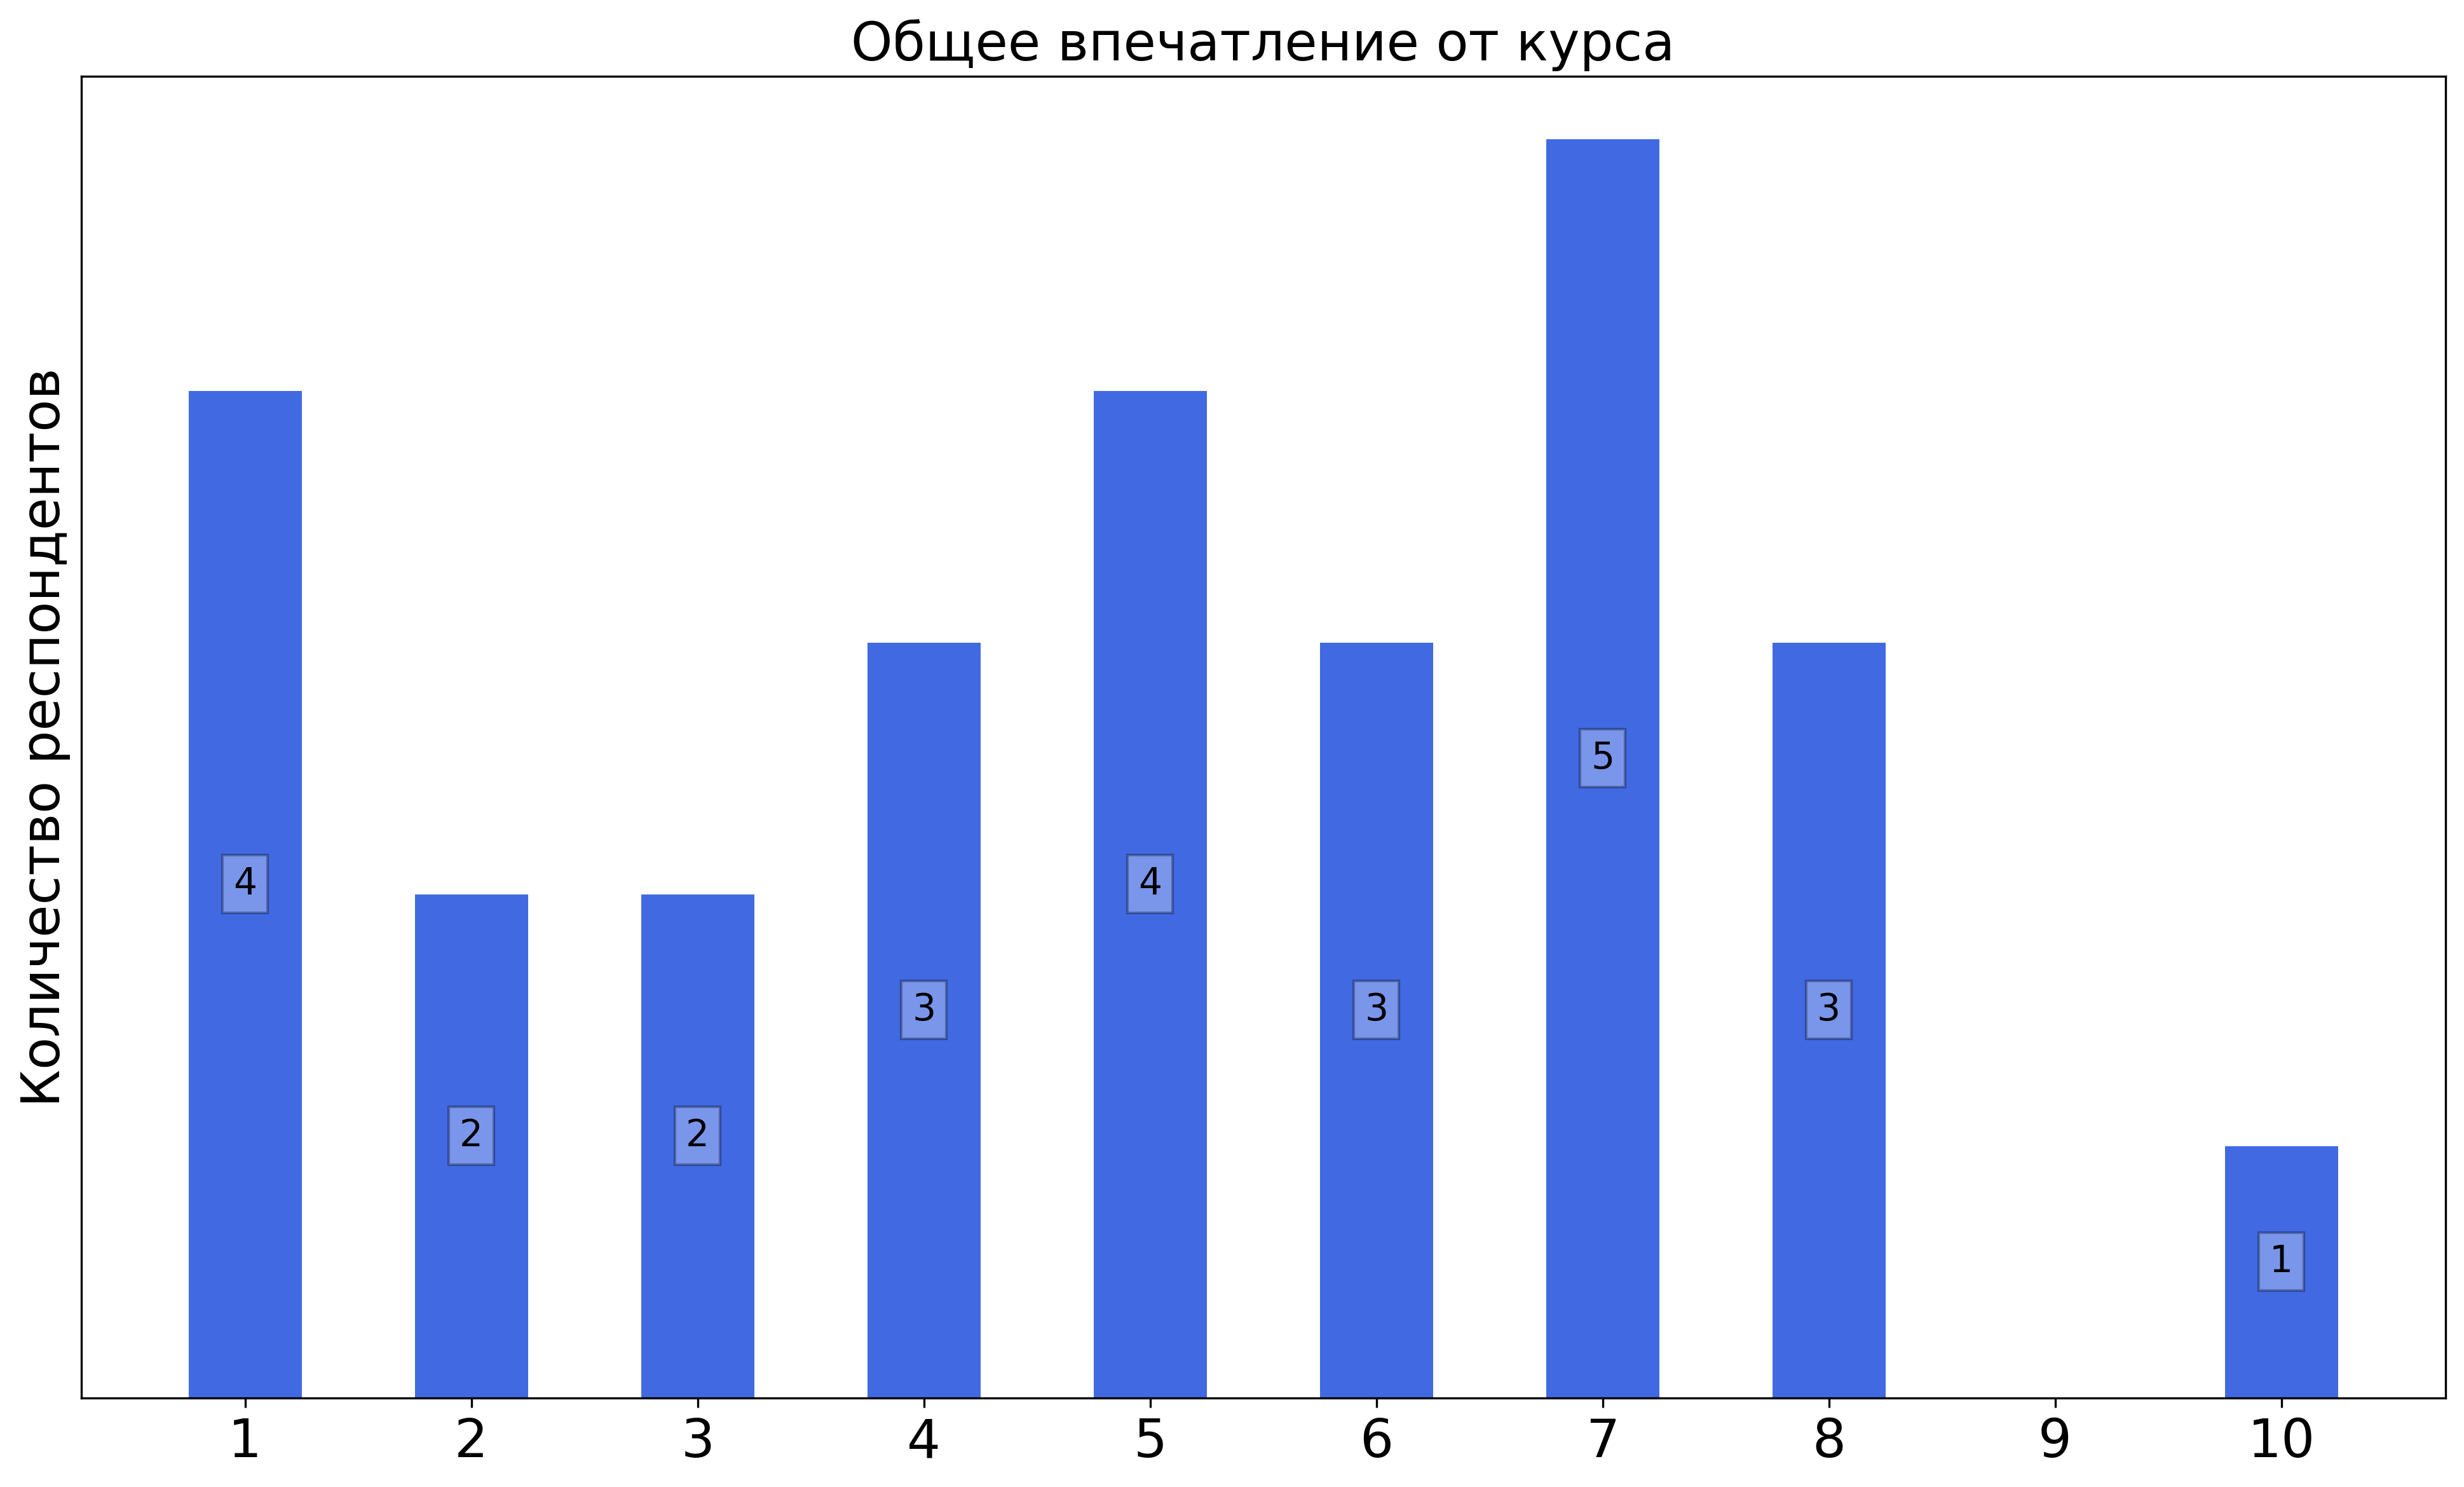
\includegraphics[width=\textwidth]{images/2 course/Радиотехнические цепи и сигналы/general-0.png}
			\end{subfigure}
			\begin{subfigure}[b]{0.45\textwidth}
				\centering
				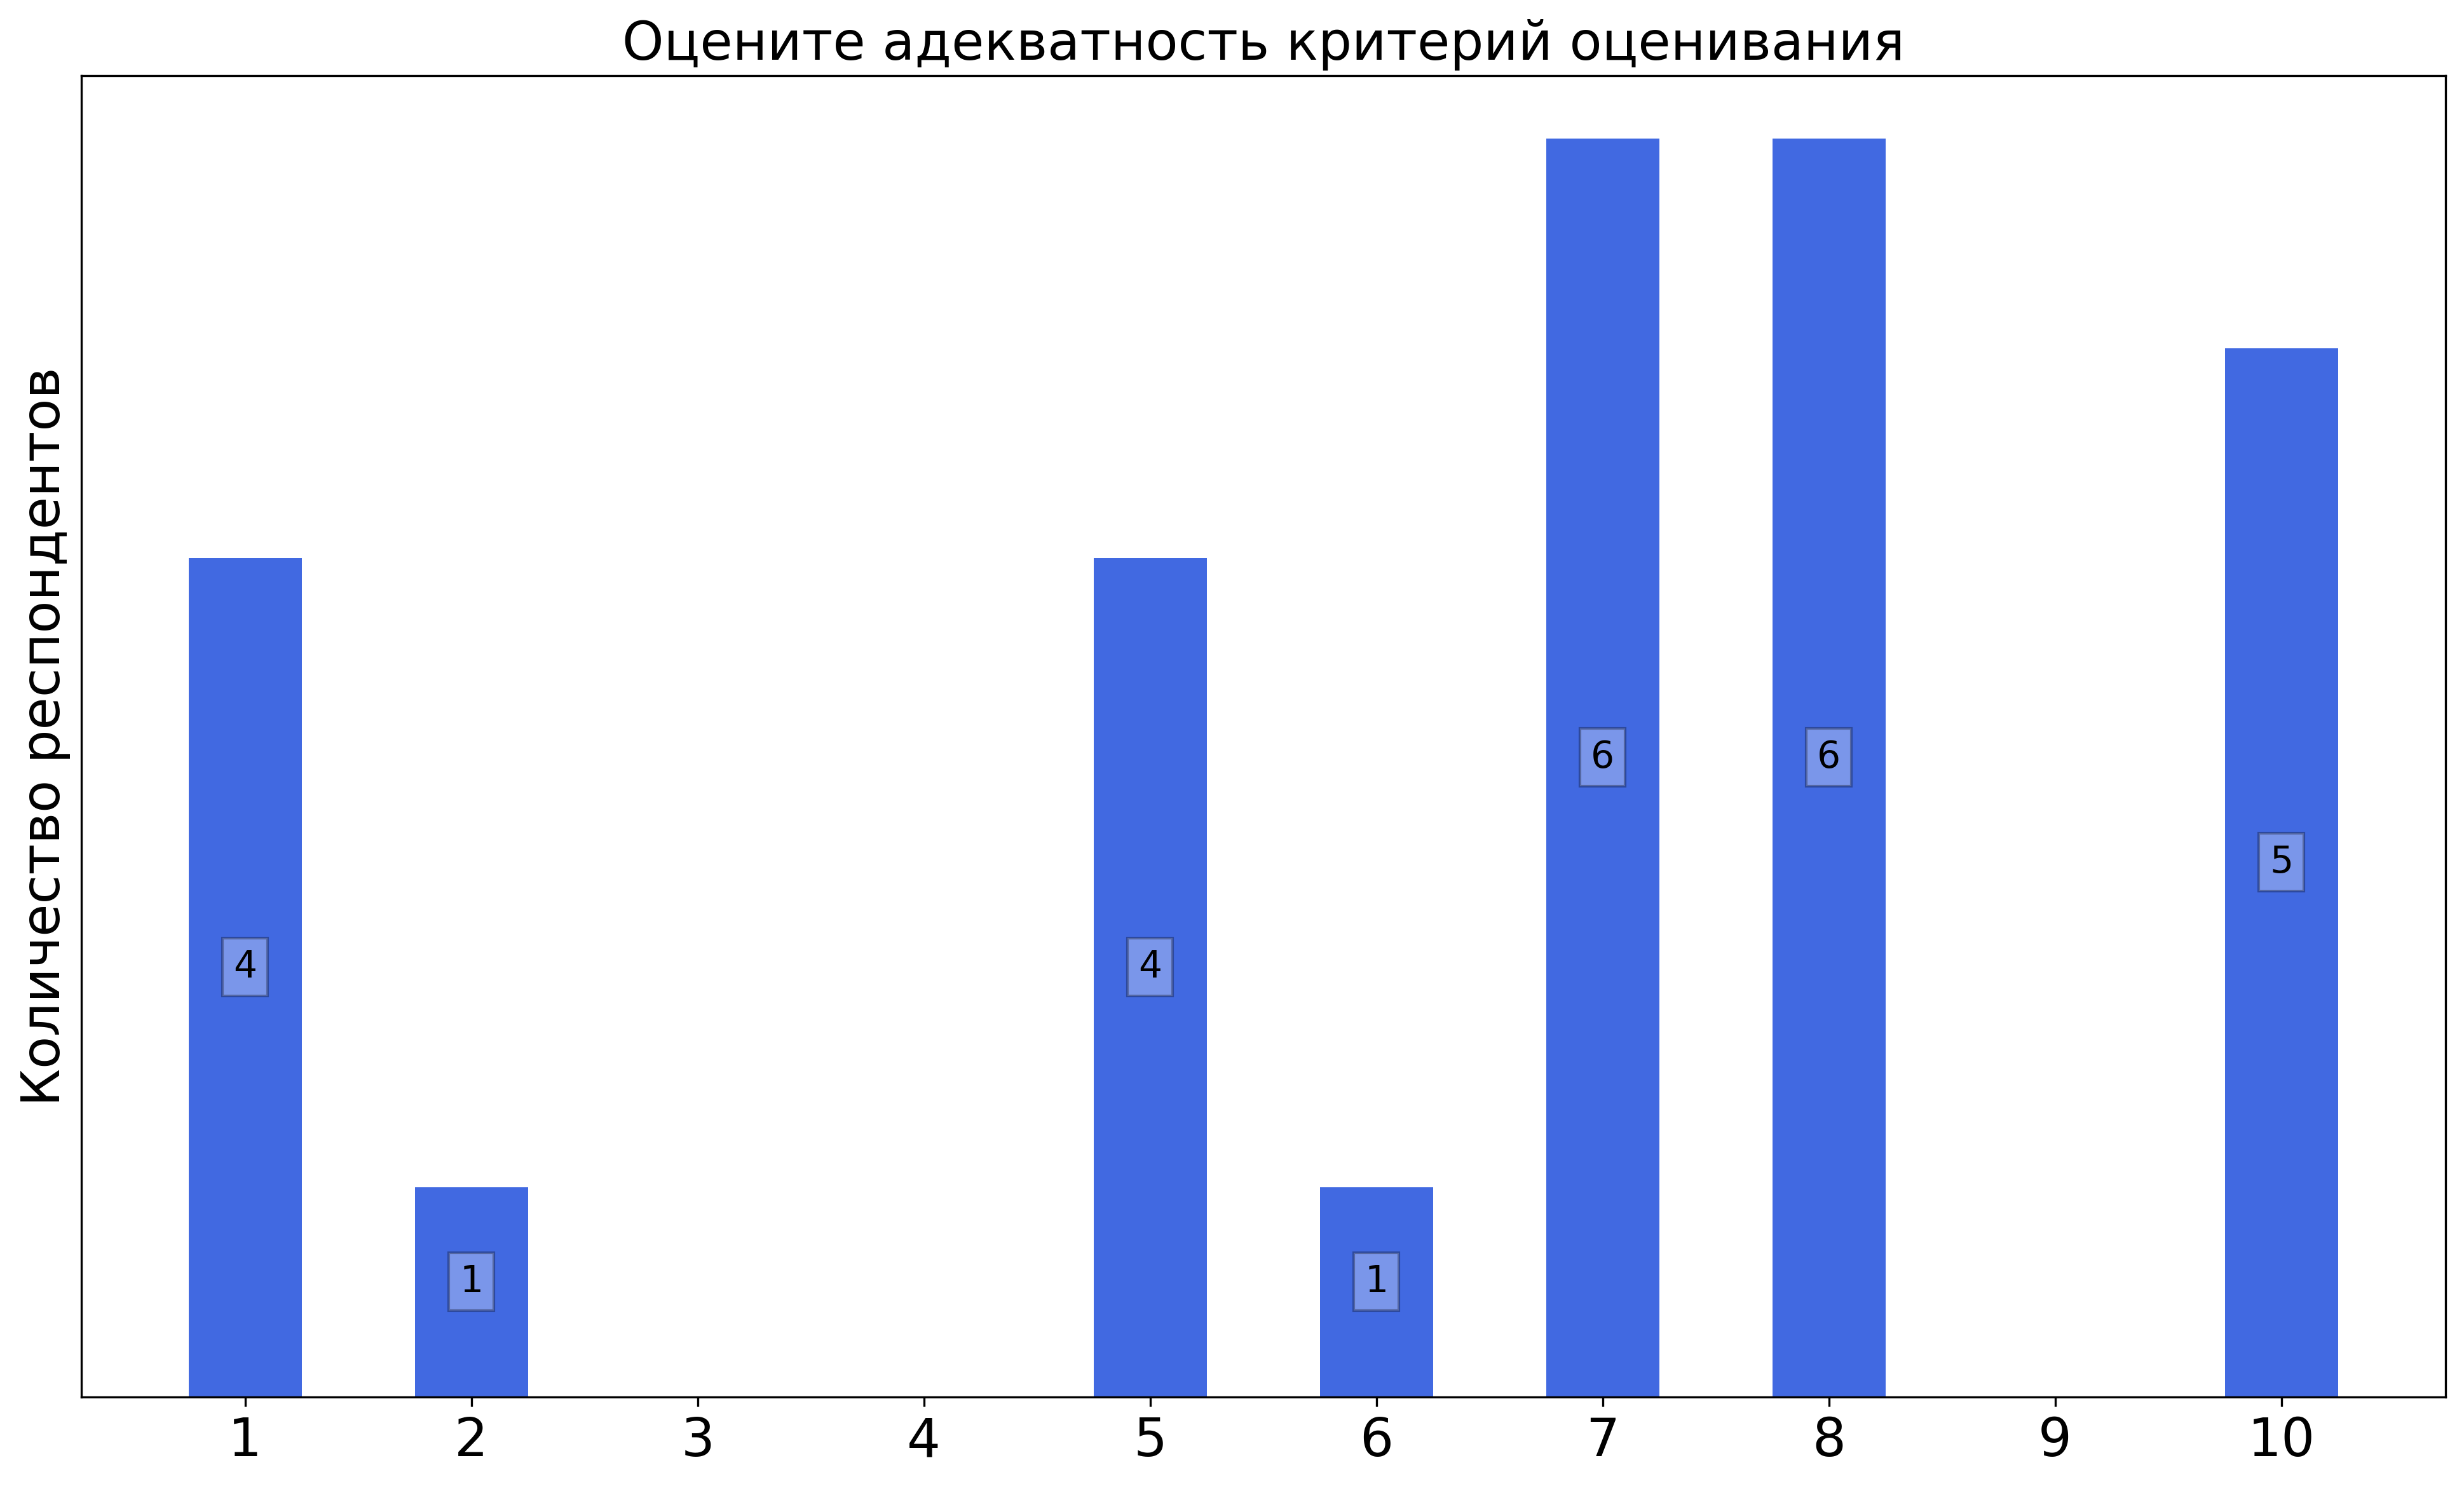
\includegraphics[width=\textwidth]{images/2 course/Радиотехнические цепи и сигналы/general-1.png}
			\end{subfigure}	
		\end{figure}

	\subsubsection{Материалы, использумые респондентами при изучении курса}

		\begin{figure}[H]
			\centering
			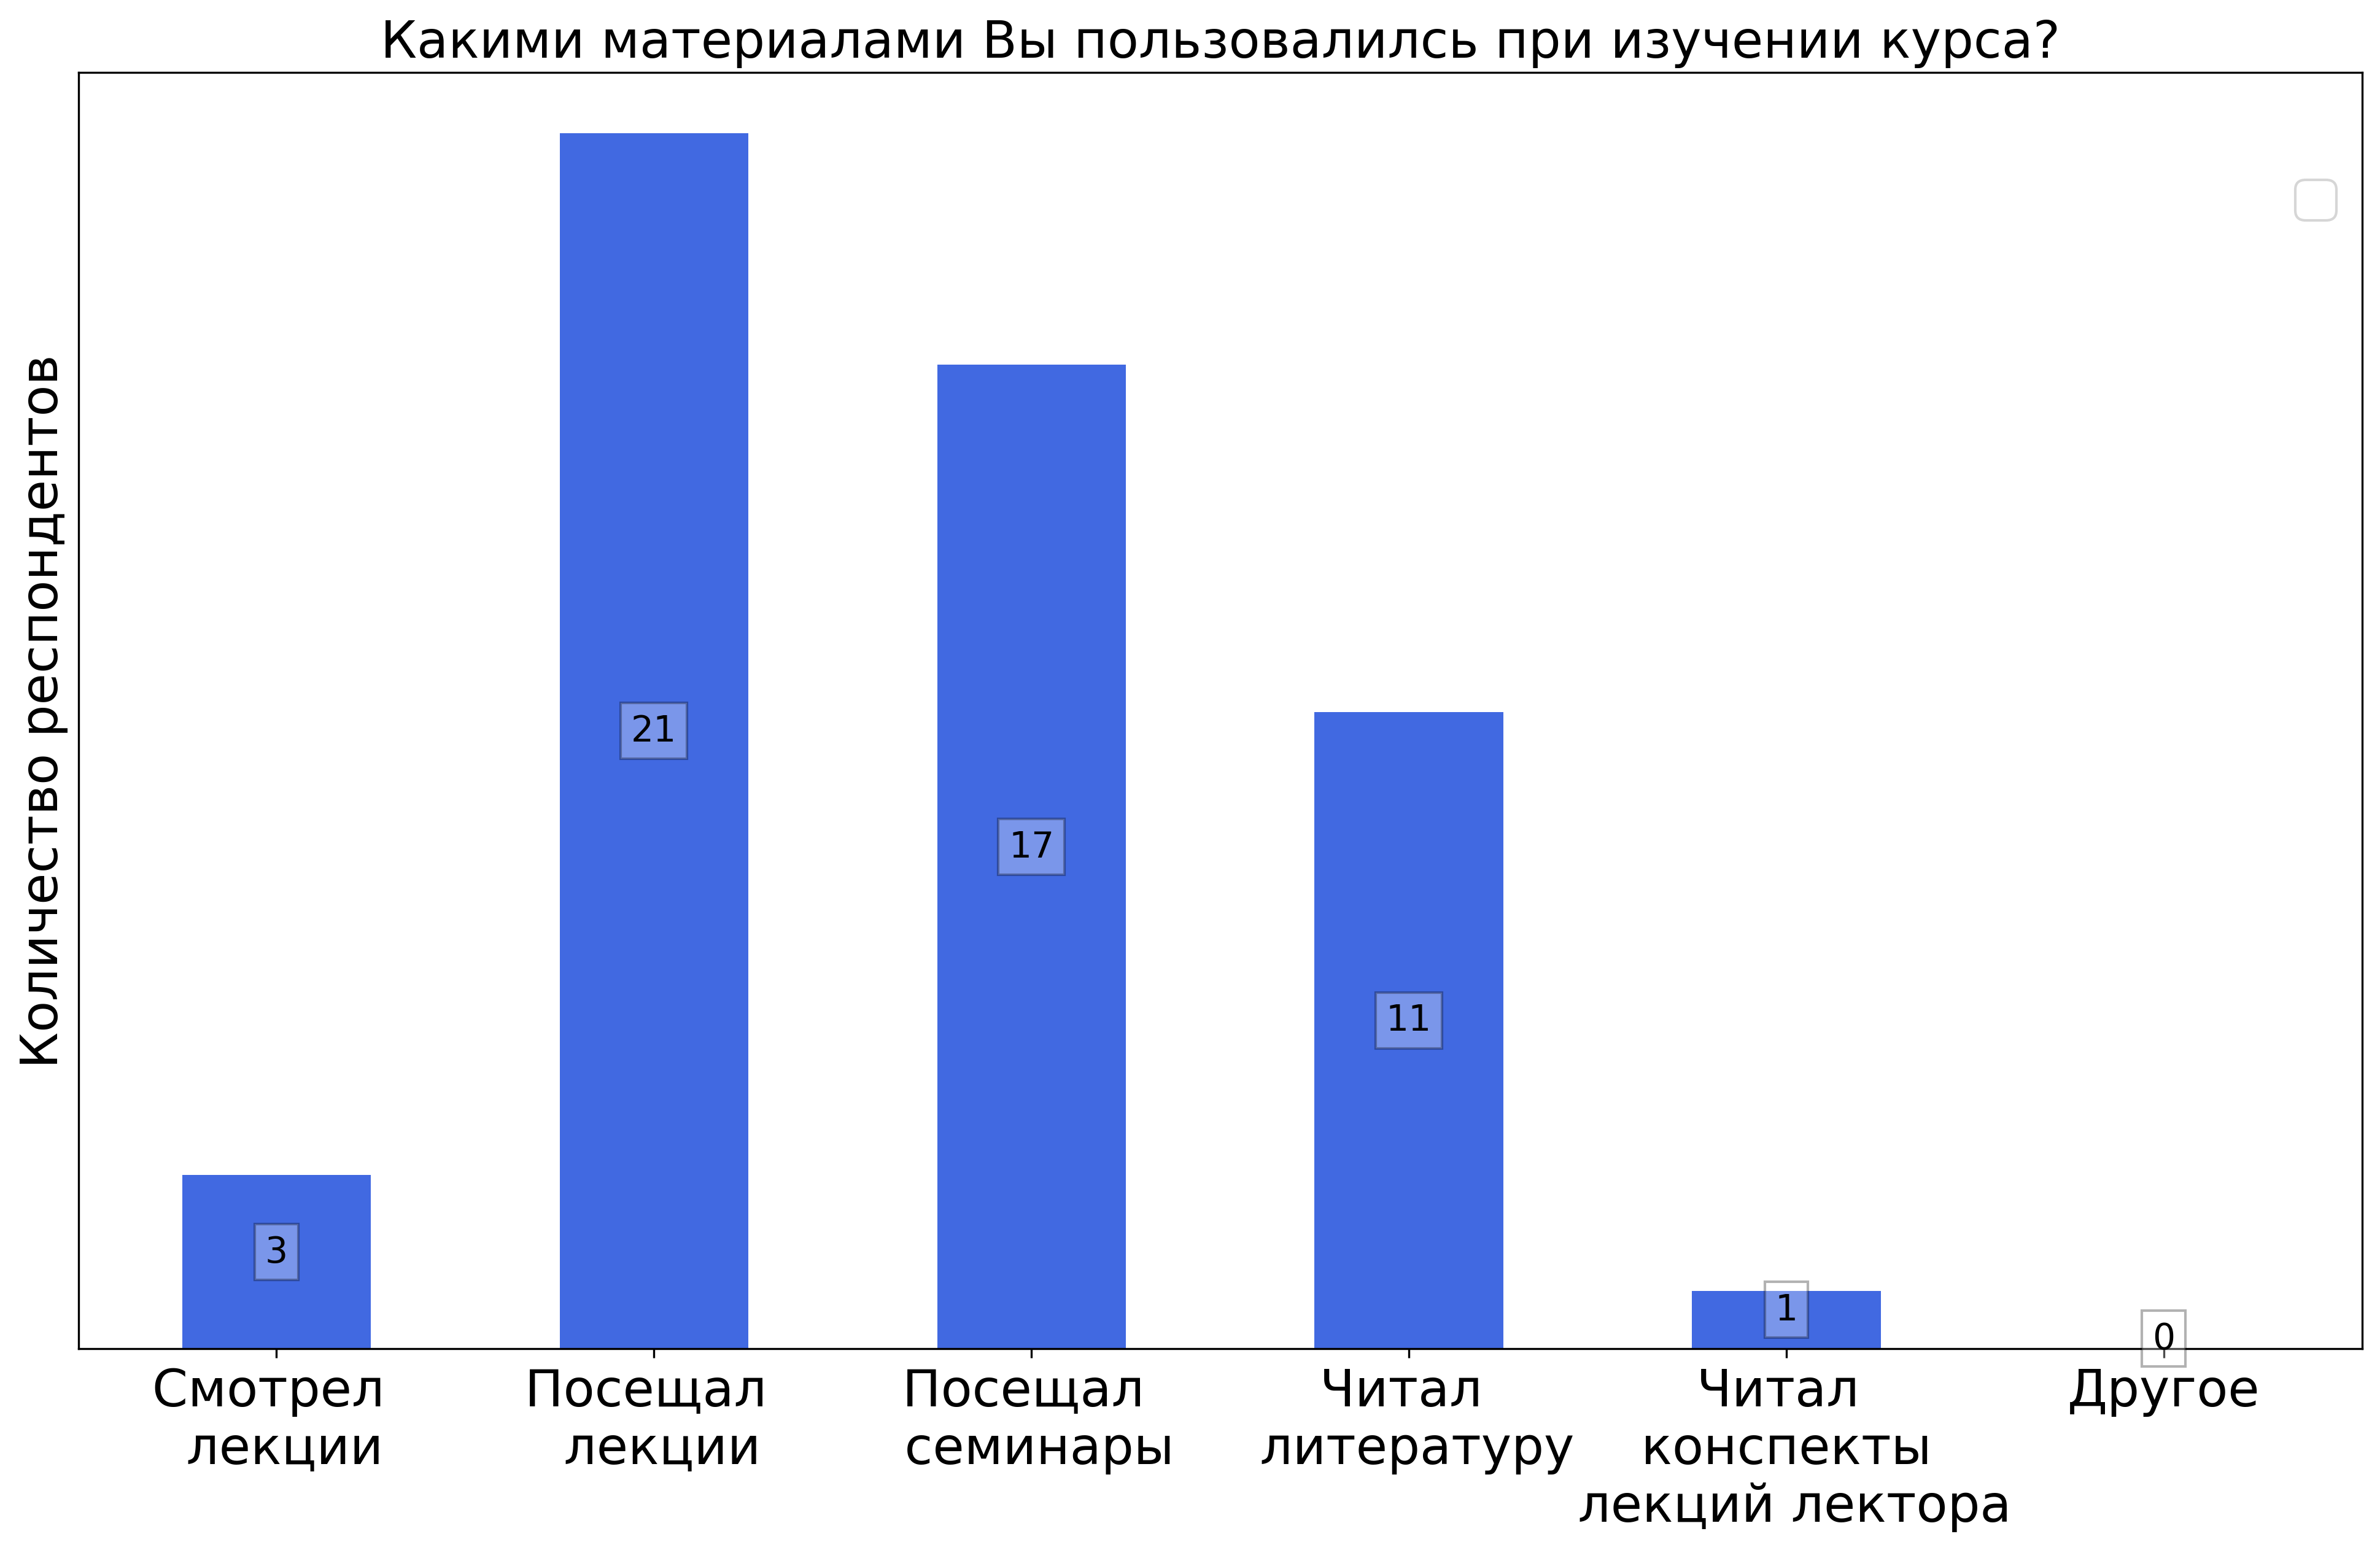
\includegraphics[width = 0.45\textwidth]{images/2 course/Радиотехнические цепи и сигналы/materials.png}
		\end{figure}

	\subsubsection{Отзыв студентов о лекциях. Лектор: Филатов И.В.}

		\begin{figure}[H]
			\centering
            \begin{subfigure}[b]{0.45\textwidth}
				\centering
				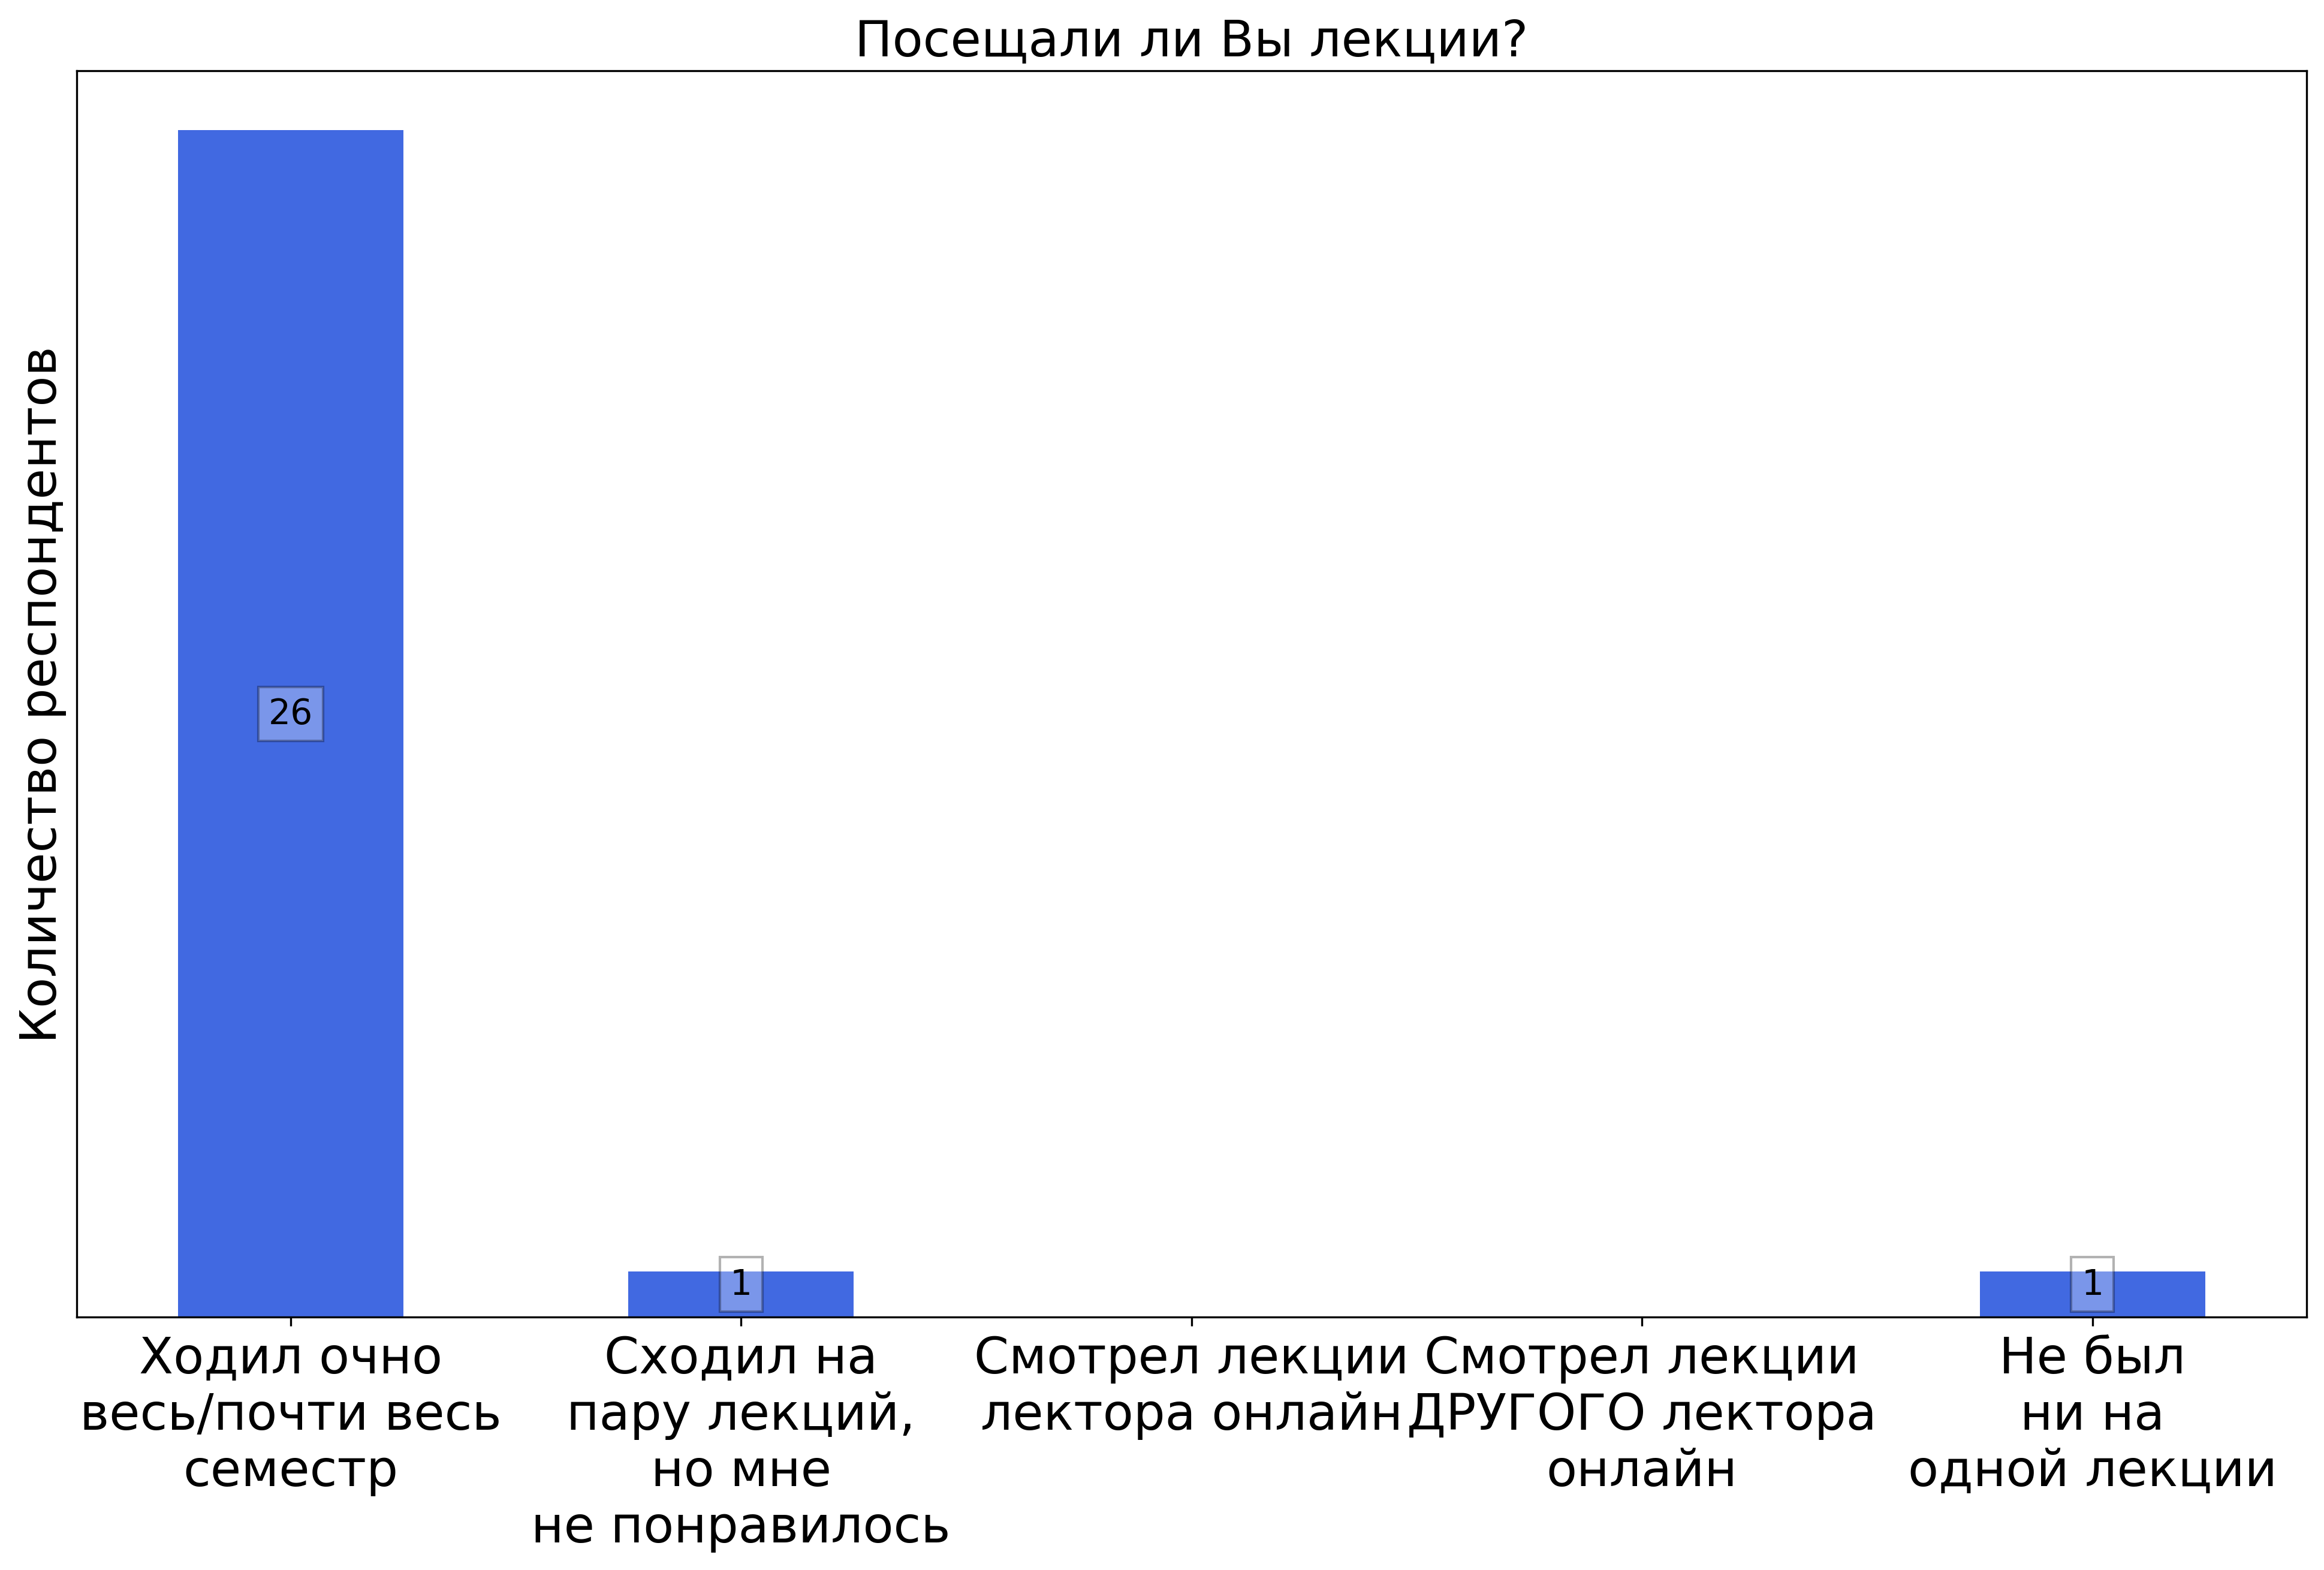
\includegraphics[width=\textwidth]{images/2 course/Радиотехнические цепи и сигналы/lecturer-questions-Филатов И.В.-0.png}
			\end{subfigure}
			\begin{subfigure}[b]{0.45\textwidth}
				\centering
				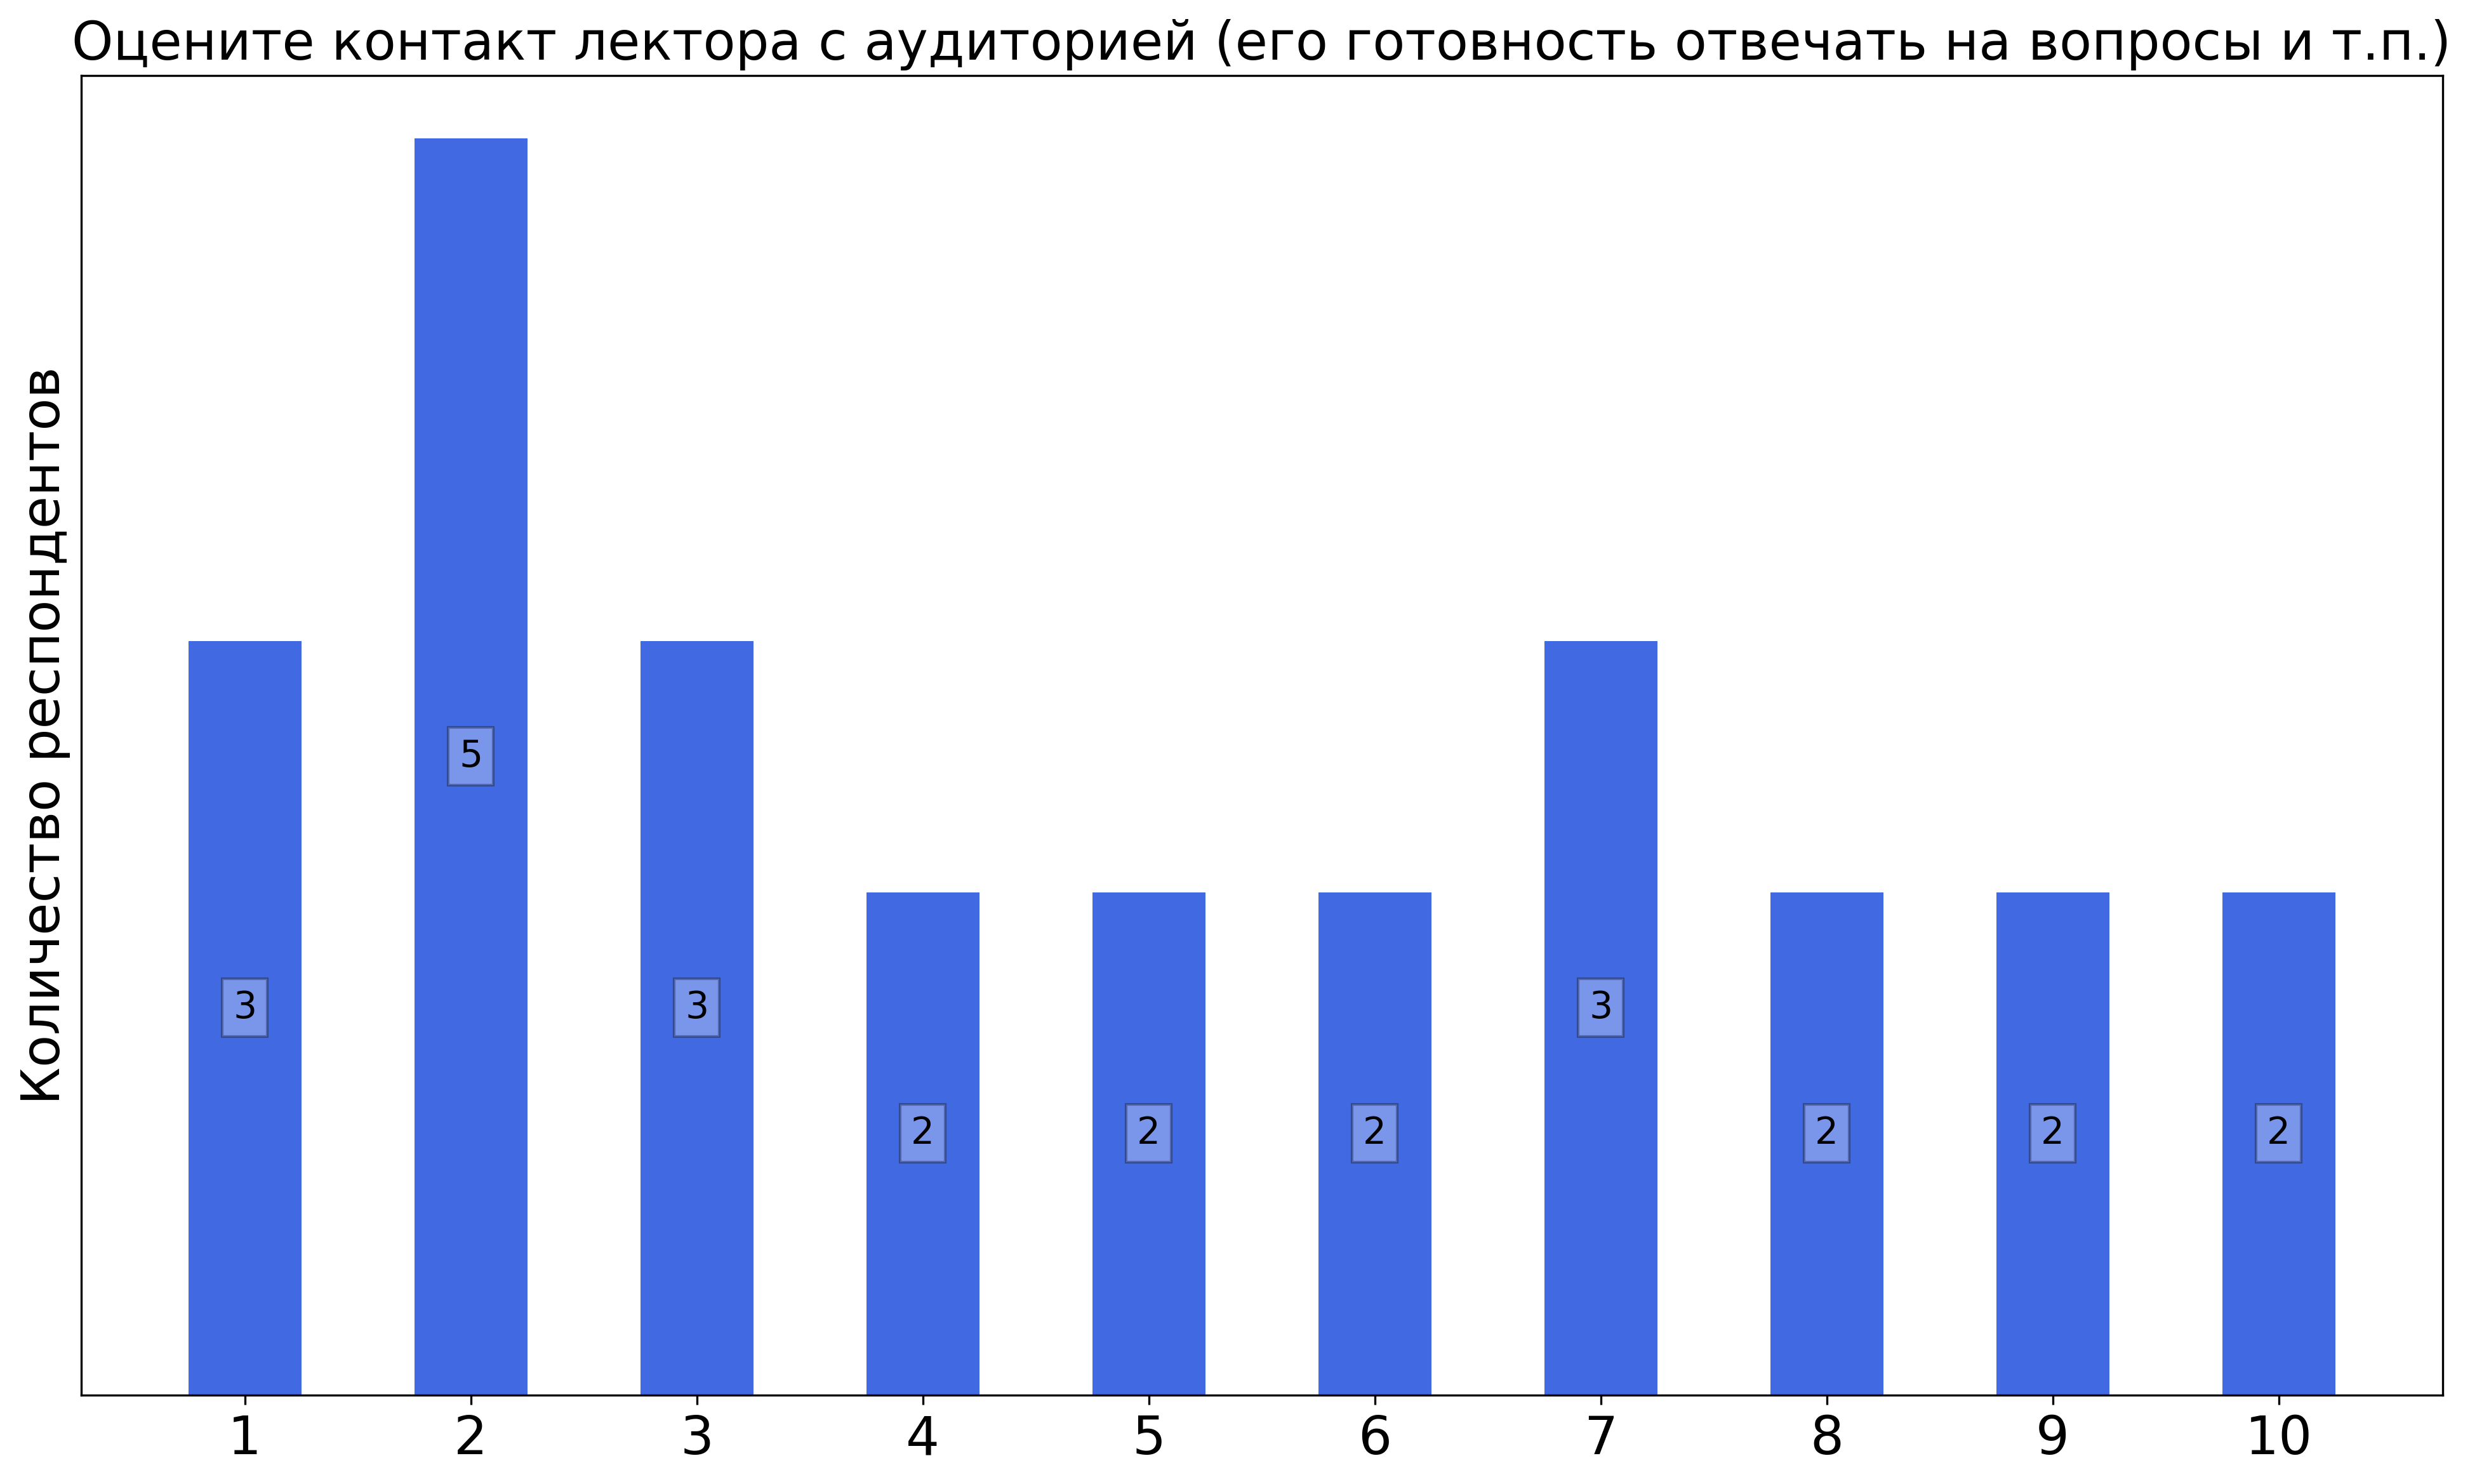
\includegraphics[width=\textwidth]{images/2 course/Радиотехнические цепи и сигналы/lecturer-marks-Филатов И.В.-0.png}
			\end{subfigure}
			\begin{subfigure}[b]{0.45\textwidth}
				\centering
				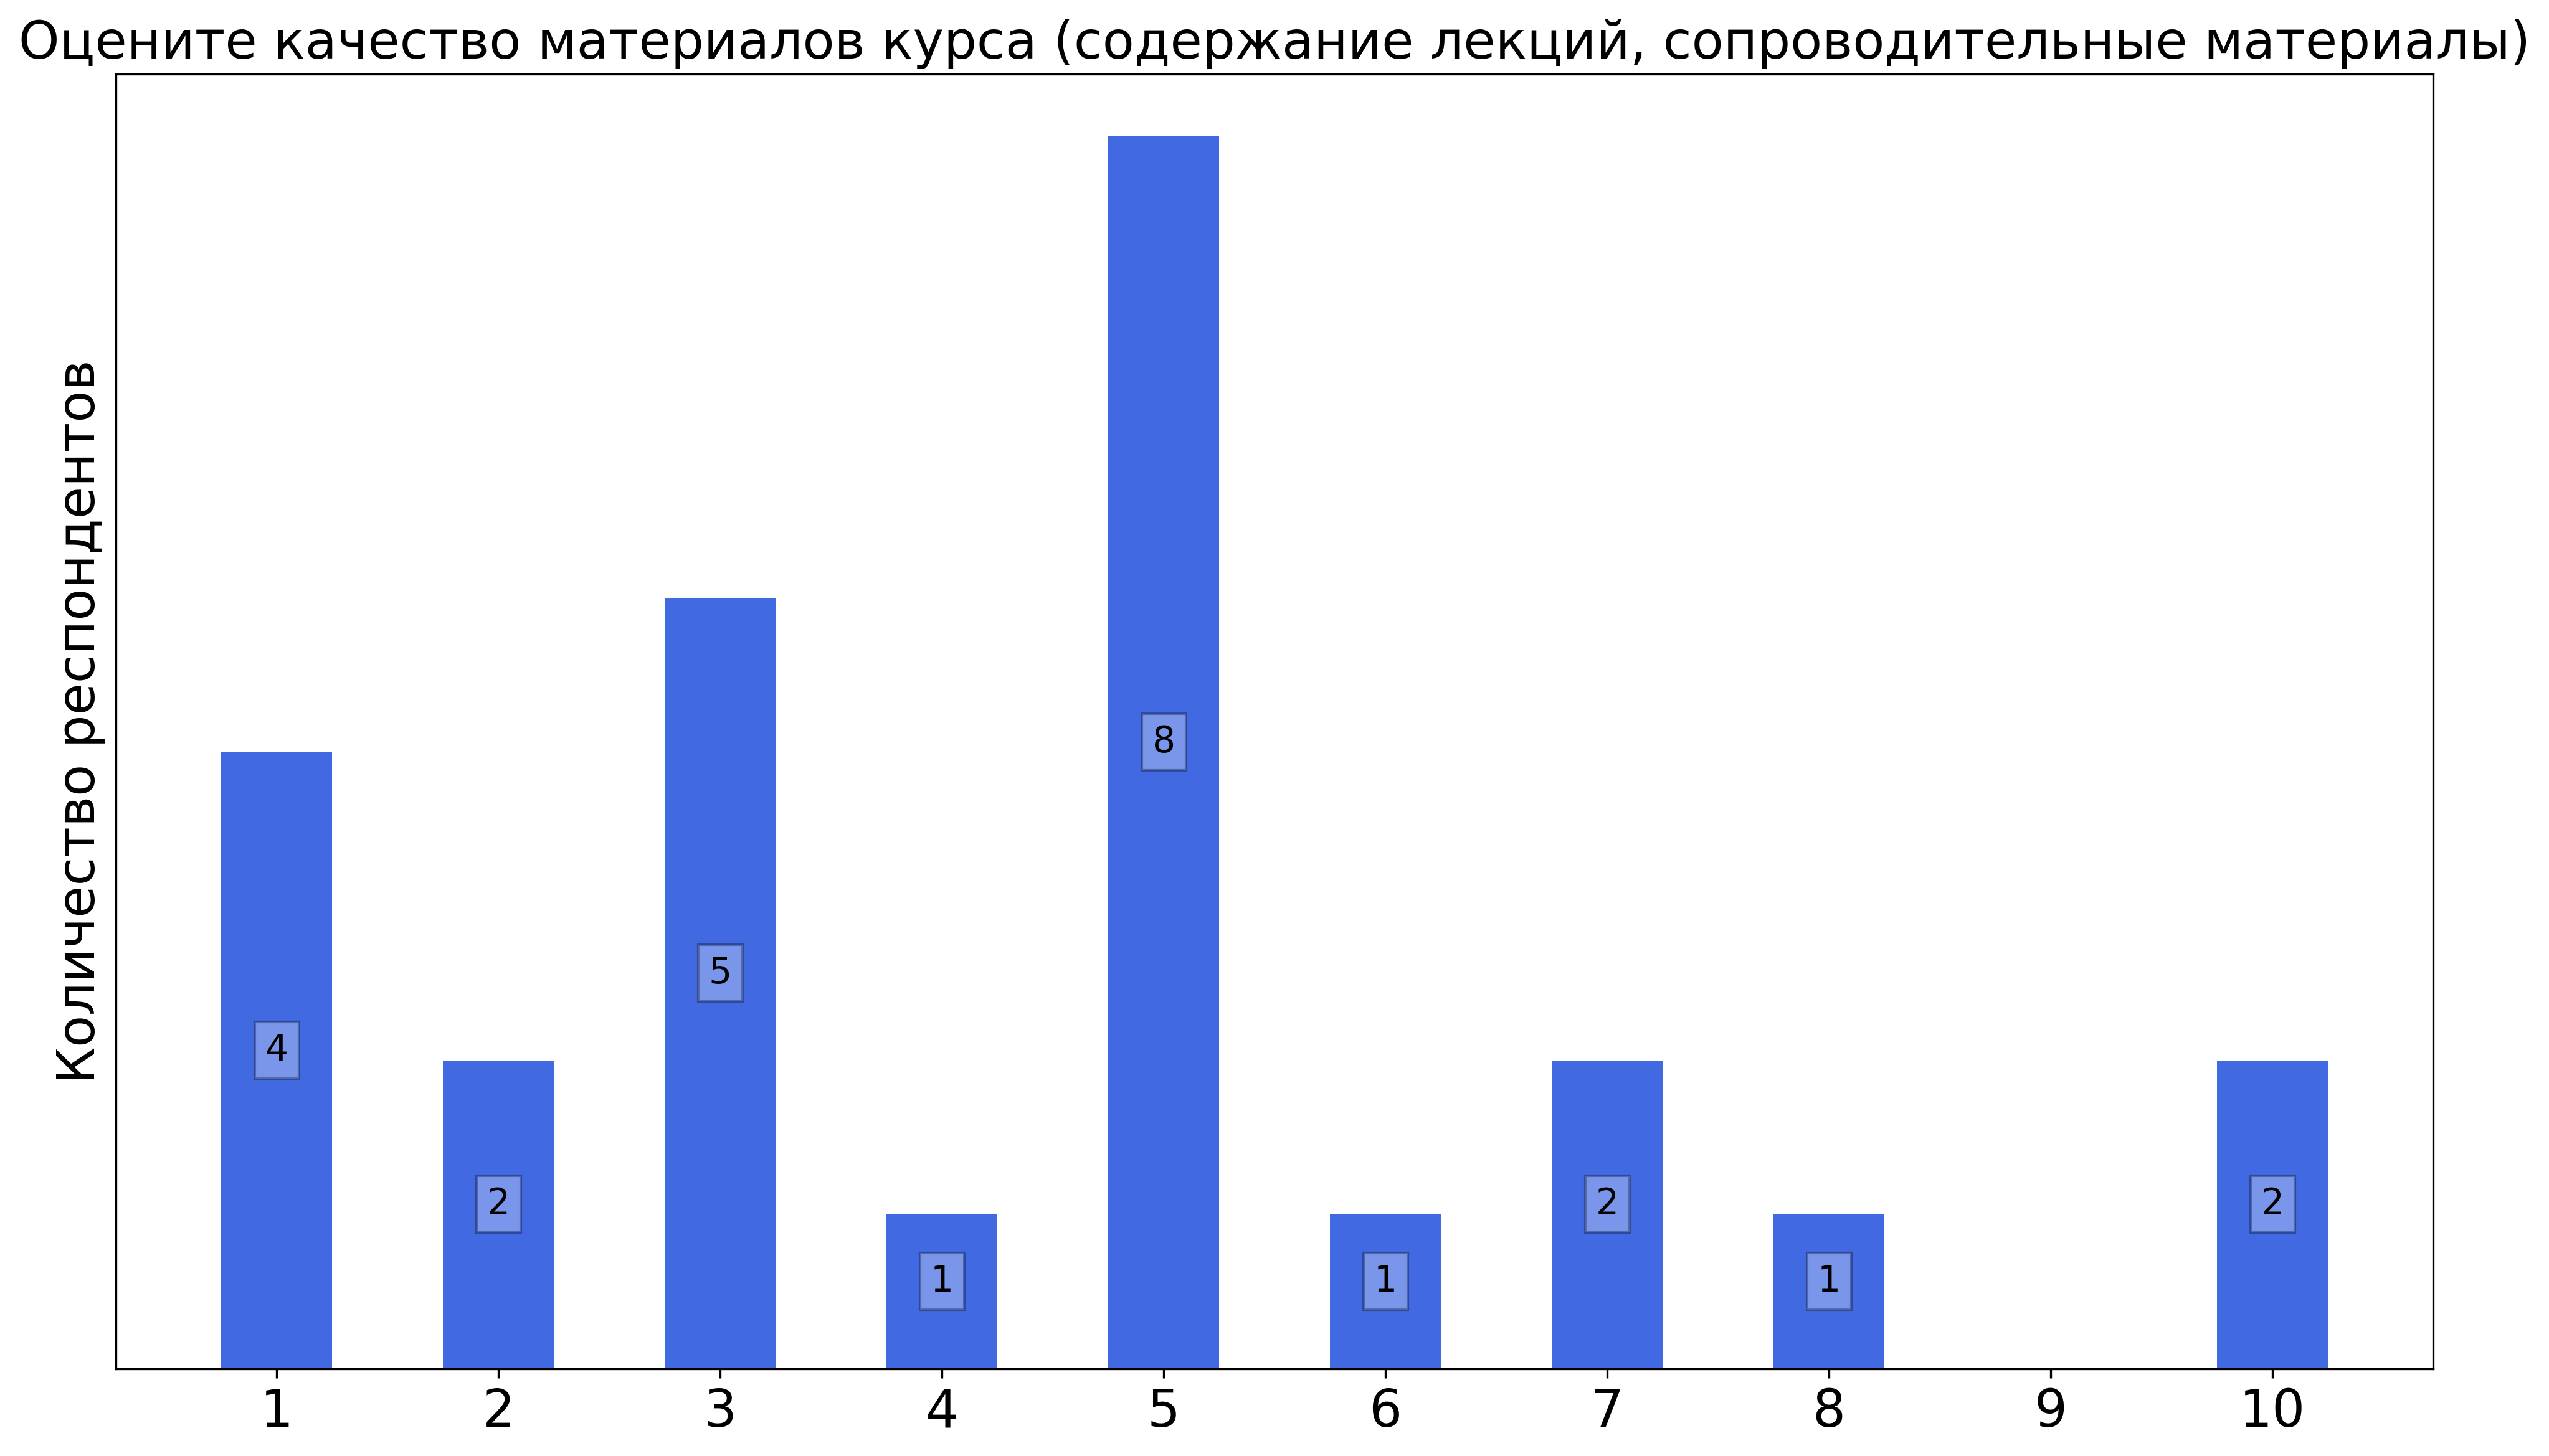
\includegraphics[width=\textwidth]{images/2 course/Радиотехнические цепи и сигналы/lecturer-marks-Филатов И.В.-1.png}
			\end{subfigure}
			\begin{subfigure}[b]{0.45\textwidth}
				\centering
				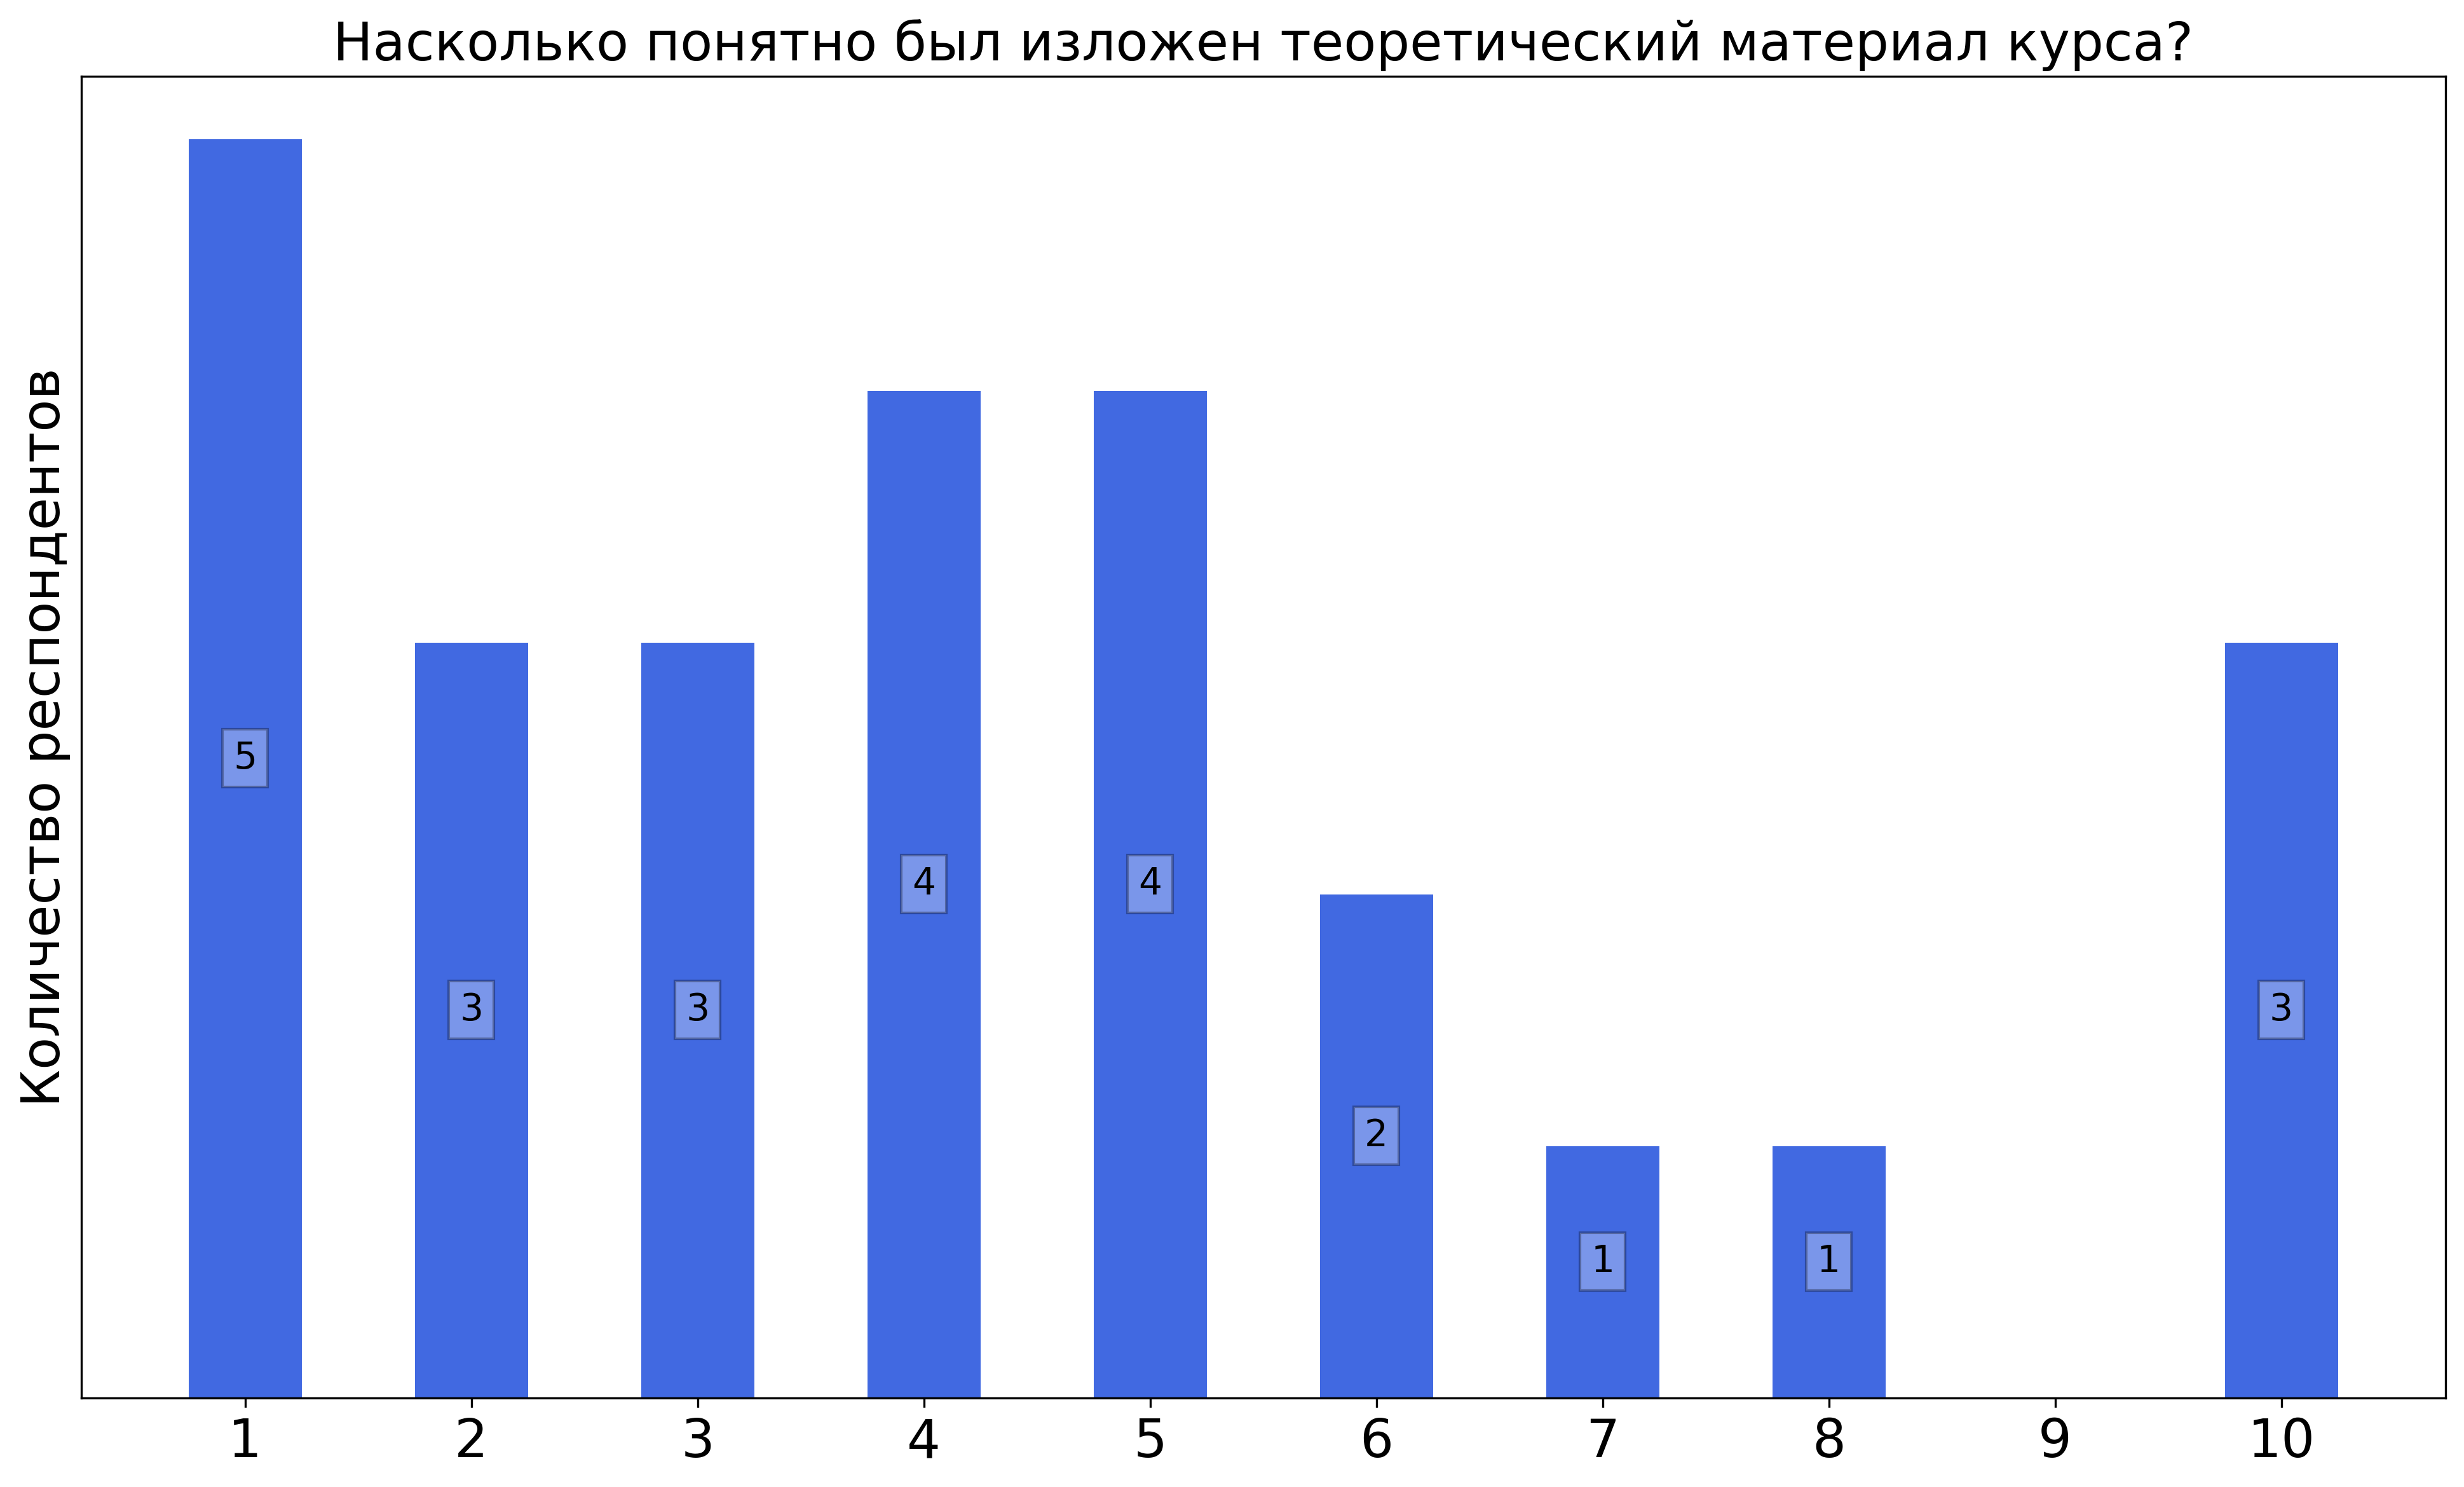
\includegraphics[width=\textwidth]{images/2 course/Радиотехнические цепи и сигналы/lecturer-marks-Филатов И.В.-2.png}
			\end{subfigure}	
			\begin{subfigure}[b]{0.45\textwidth}
				\centering
				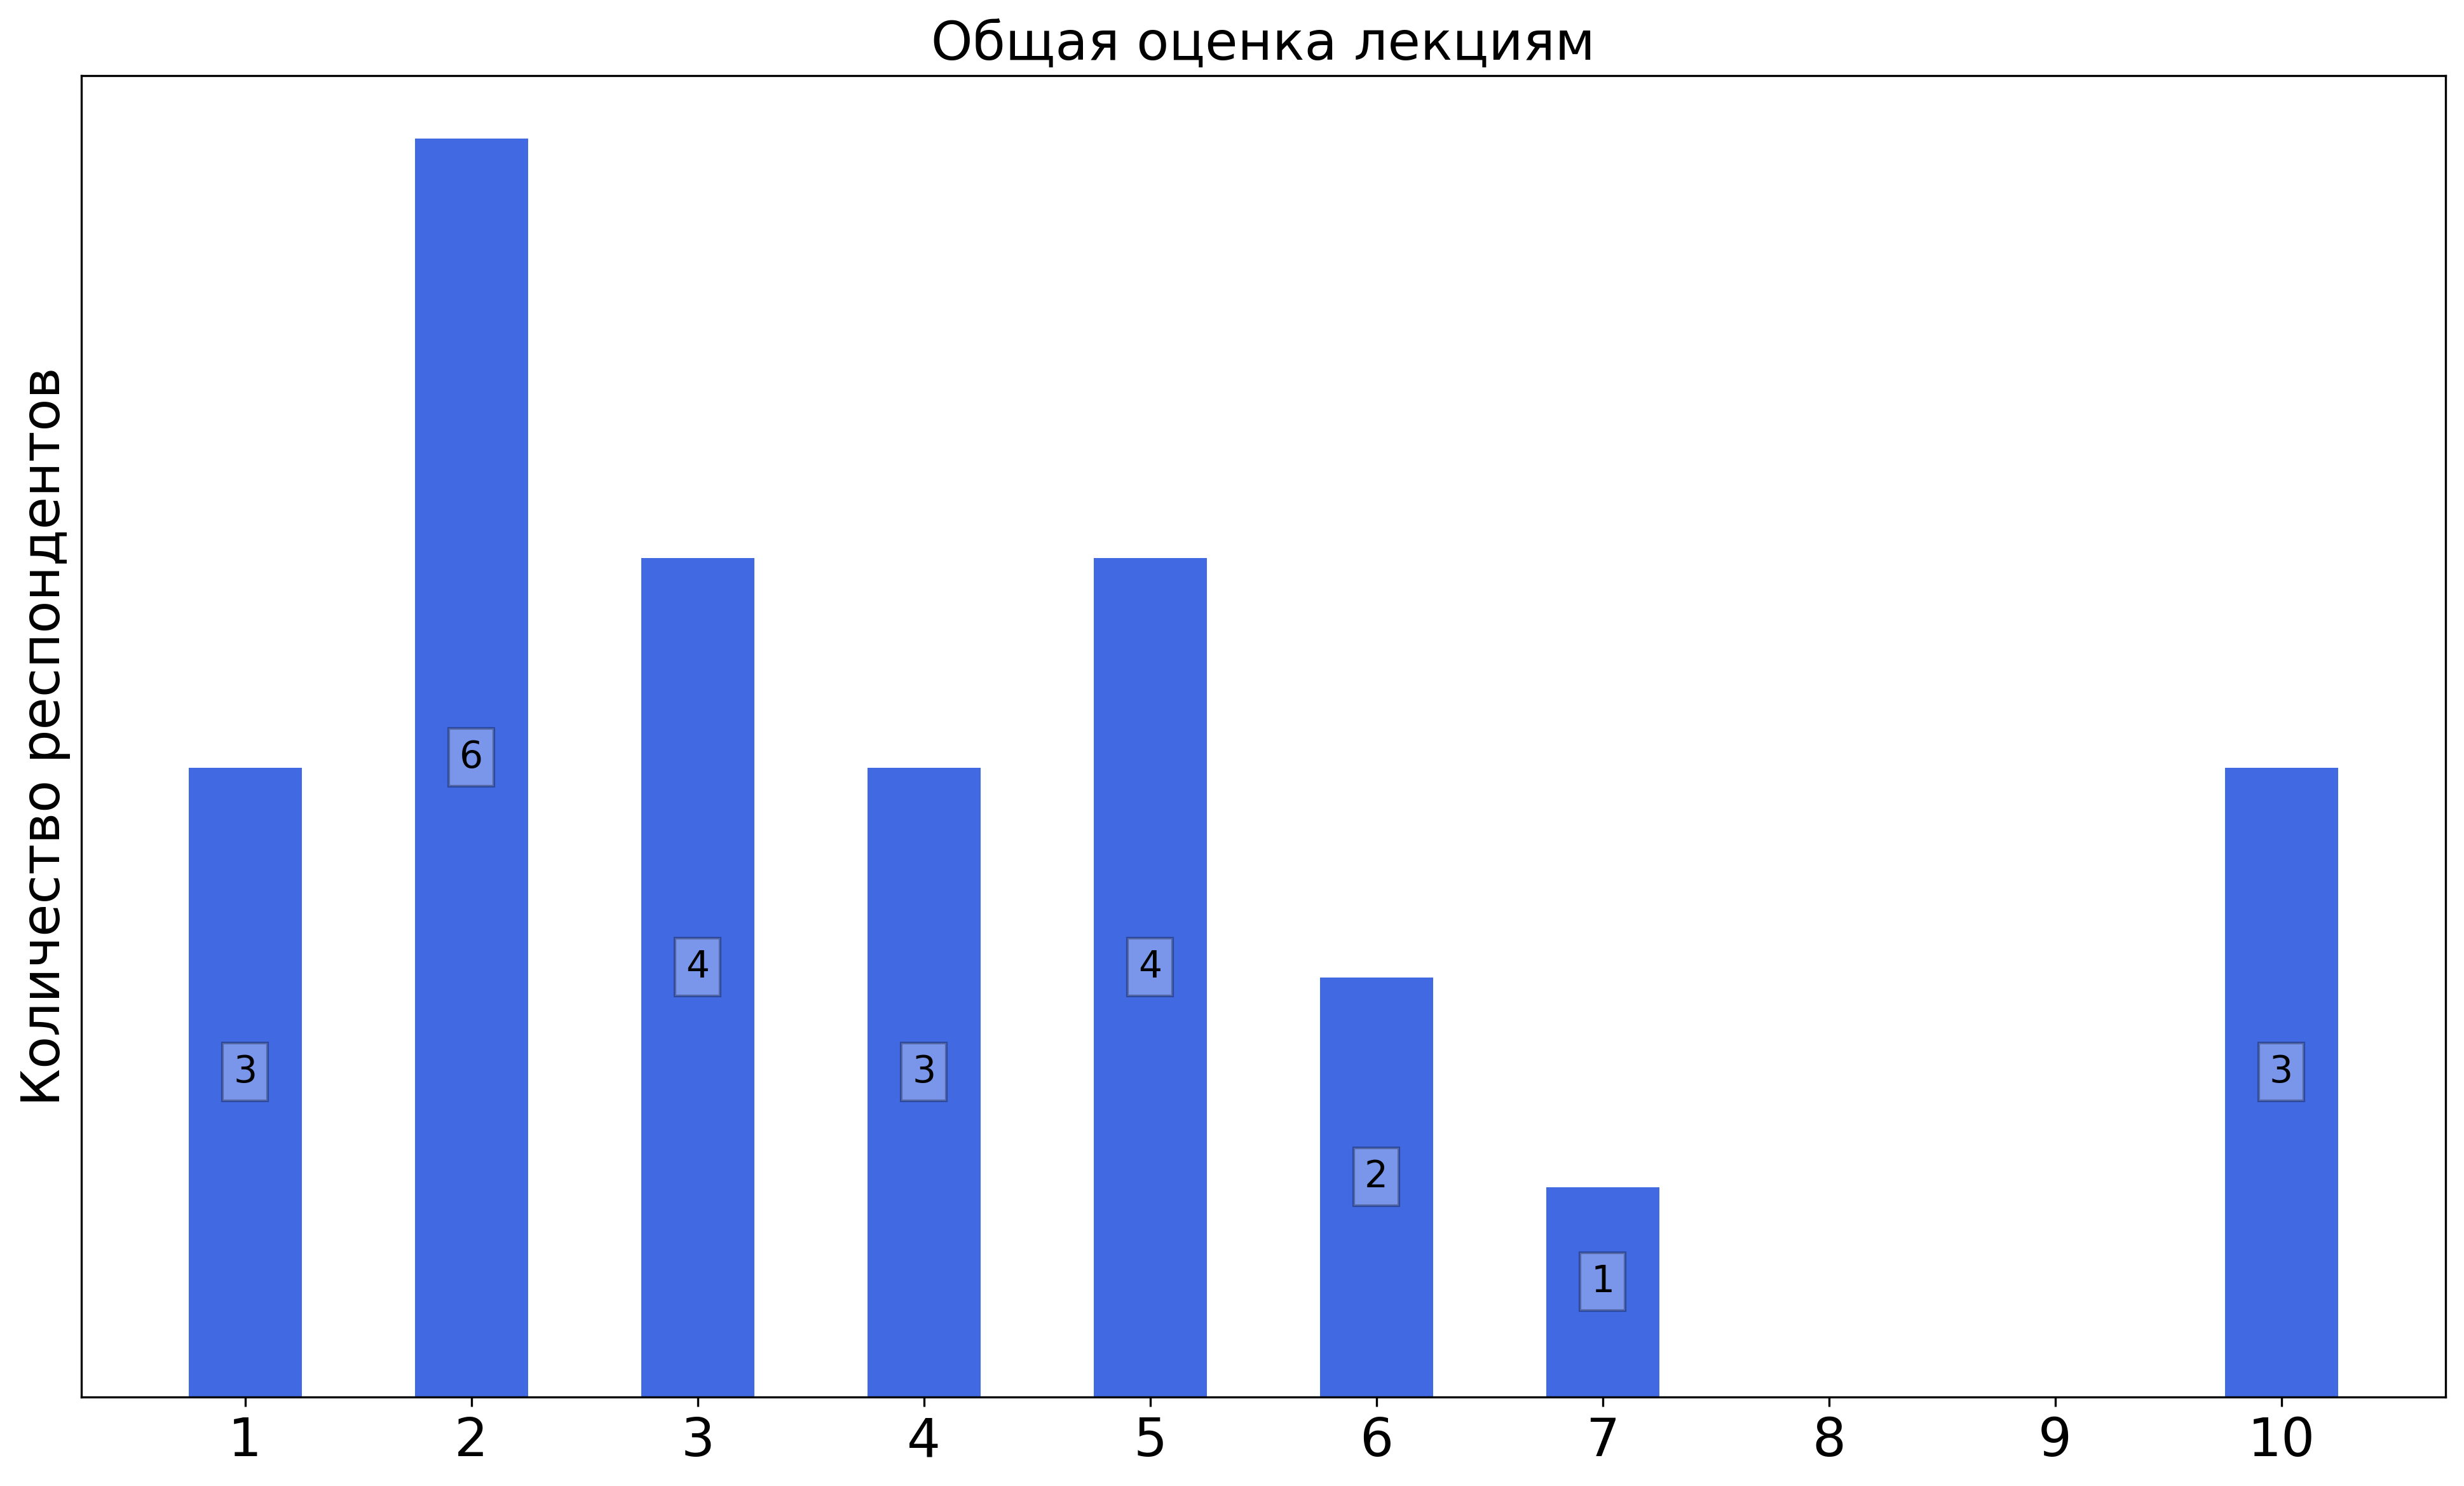
\includegraphics[width=\textwidth]{images/2 course/Радиотехнические цепи и сигналы/lecturer-marks-Филатов И.В.-3.png}
			\end{subfigure}
			\caption{Оценки респондентов о качестве преподавания лекций по курсу <<Радиотехнические цепи и сигналы>>}
		\end{figure}

		\textbf{Комментарии студентов о лекциях\protect\footnote{сохранены оригинальные орфография и пунктуация}}
            \begin{commentbox} 
                Лекции помогли с подготовкой к решениям задач в лабораторном практикуме   
            \end{commentbox} 
        
            \begin{commentbox} 
                После того, как препод не смог разложить синус в ряд Тейлора, я сильно разочаровался в нем. Вместо ответов на вопросы - одни метафоры
            \end{commentbox} 
        
            \begin{commentbox} 
                Не заинтересовано рассказывает о предмете, видно, что у него нет цели понятно и интересно донести материал. 
            \end{commentbox} 
        
            \begin{commentbox} 
                Не структурировано 
            \end{commentbox} 
        
            \begin{commentbox} 
                Лекции непонятны, на все вопросы Советовал погуглить. 
            \end{commentbox}  
    

    \subsubsection{Отзыв студентов о лабораторных работах. Преподаватель: Арумов Г.П.}
		\begin{figure}[H]
			\centering
			\begin{subfigure}[b]{0.45\textwidth}
				\centering
				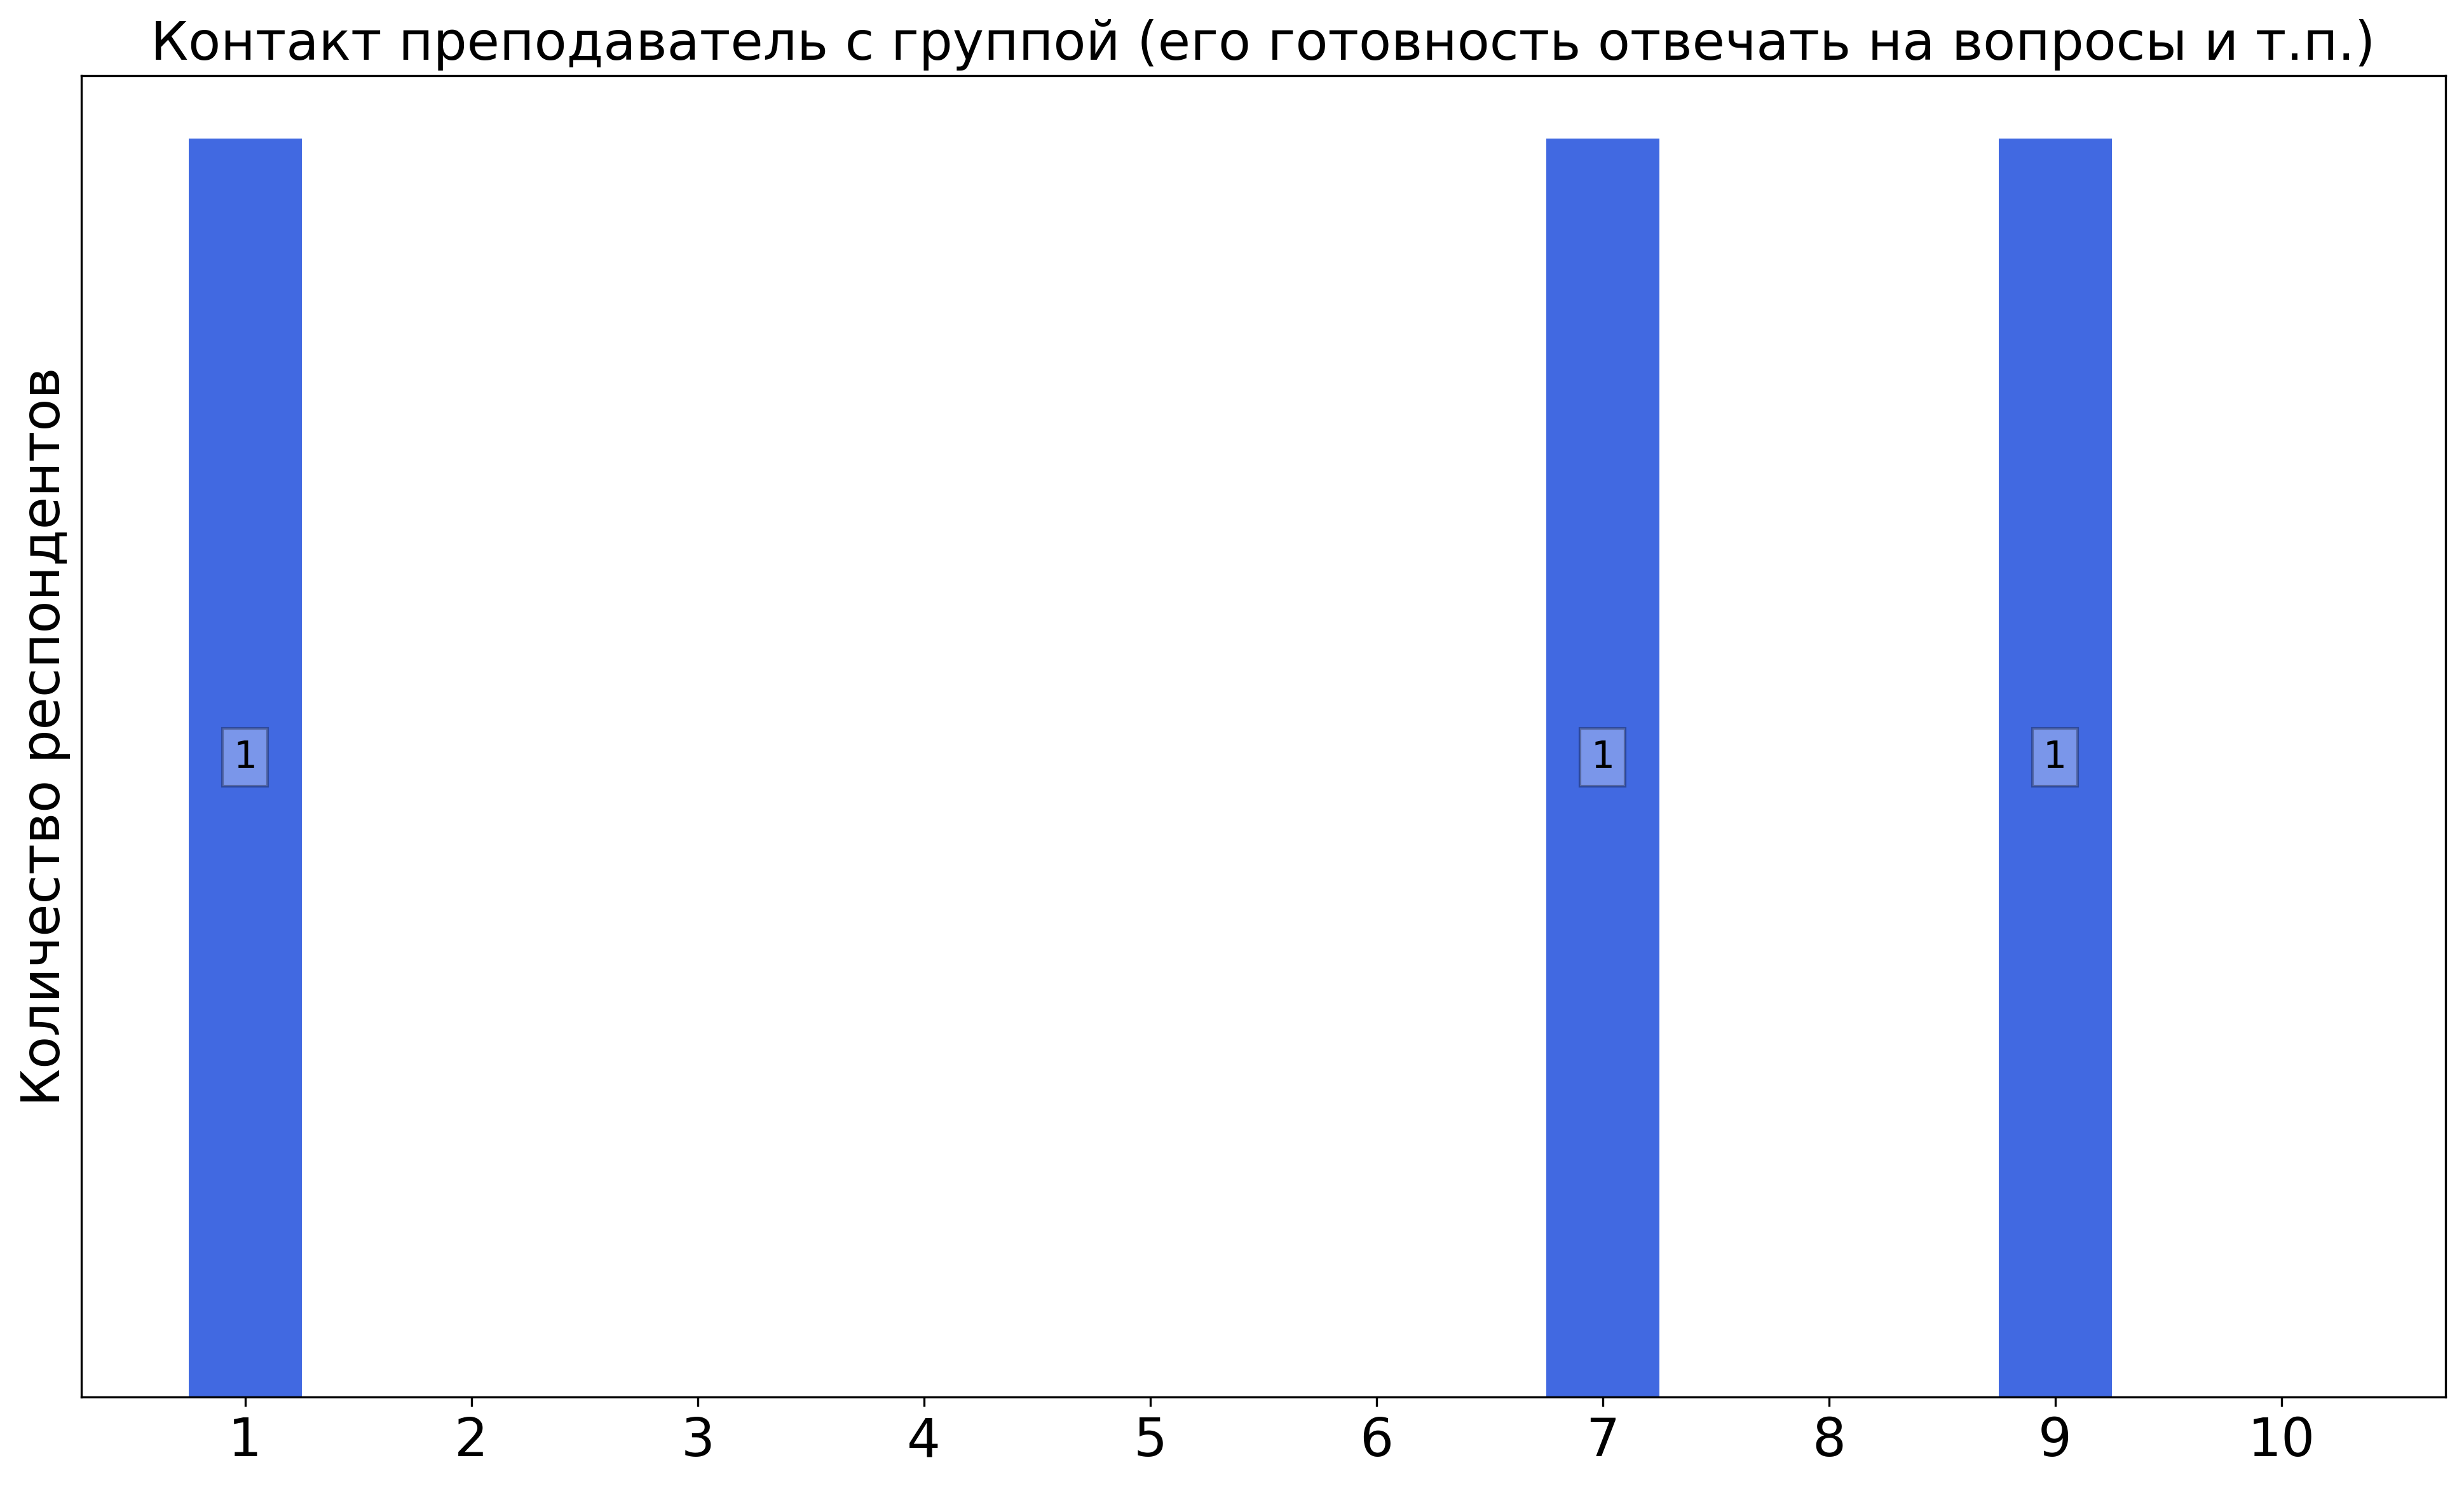
\includegraphics[width=\textwidth]{images/2 course/Радиотехнические цепи и сигналы/labniks-marks-Арумов Г.П.-0.png}
			\end{subfigure}
			\begin{subfigure}[b]{0.45\textwidth}
				\centering
				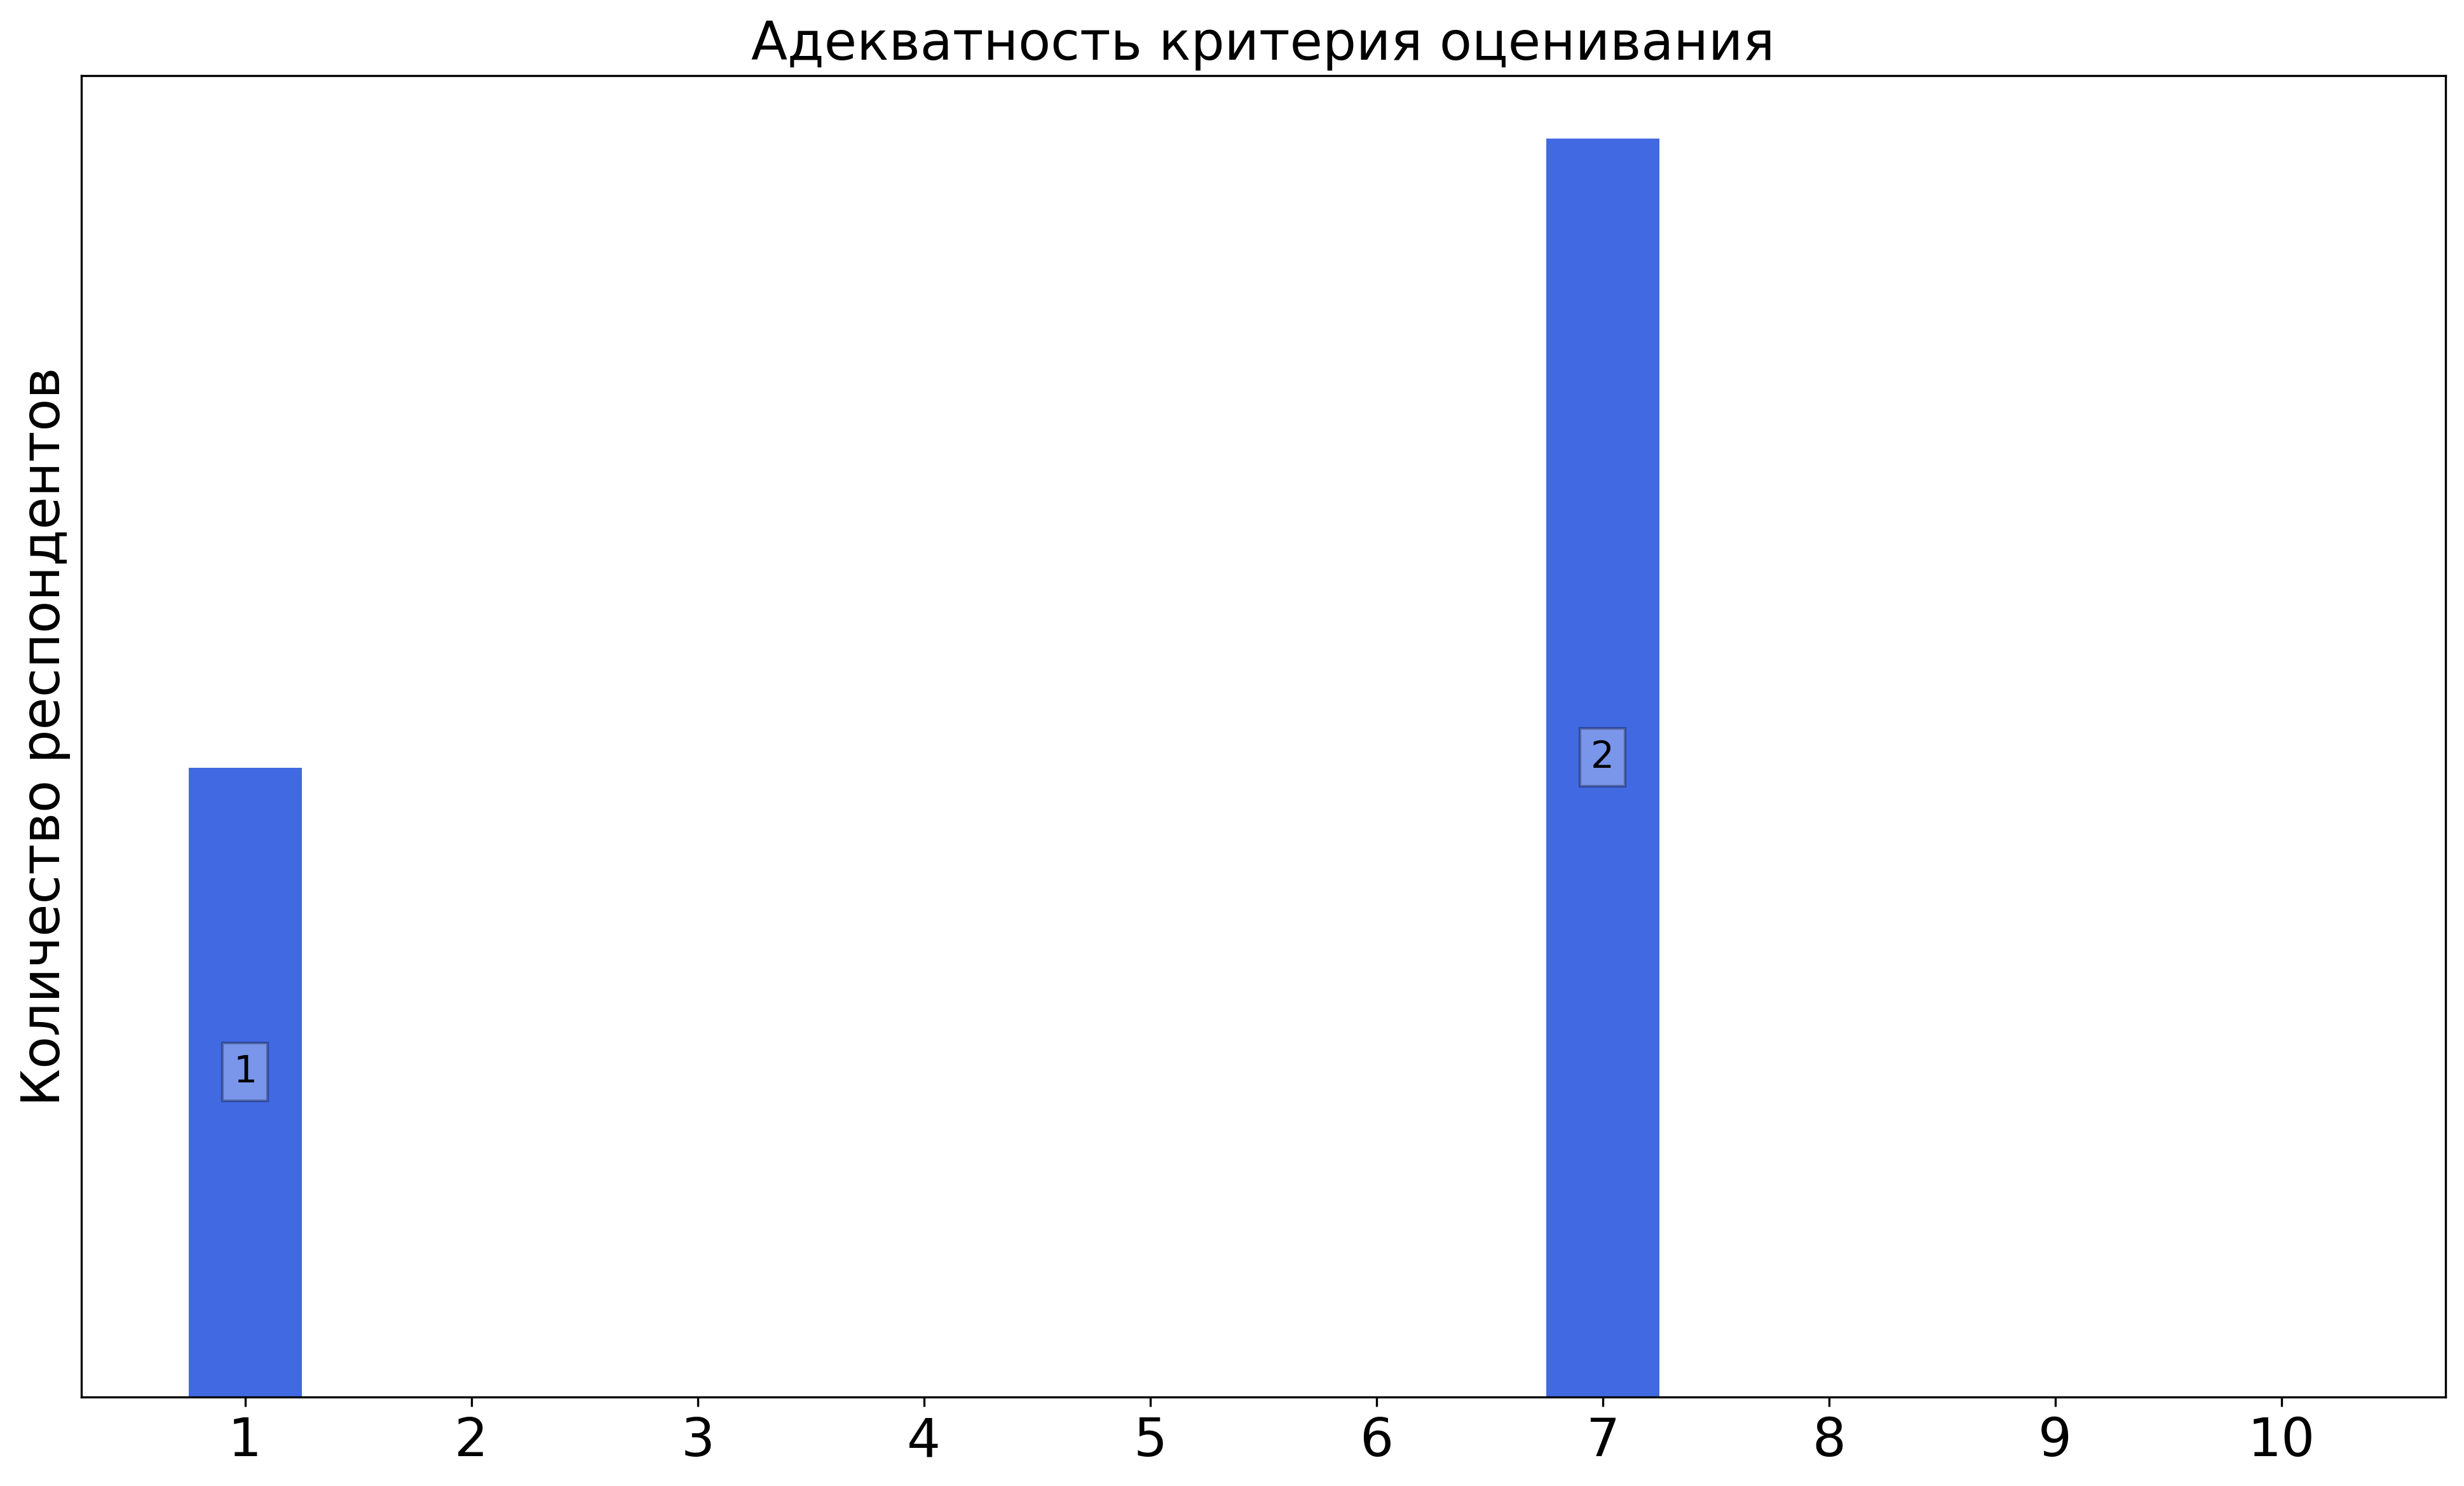
\includegraphics[width=\textwidth]{images/2 course/Радиотехнические цепи и сигналы/labniks-marks-Арумов Г.П.-1.png}
			\end{subfigure}
			\begin{subfigure}[b]{0.45\textwidth}
				\centering
				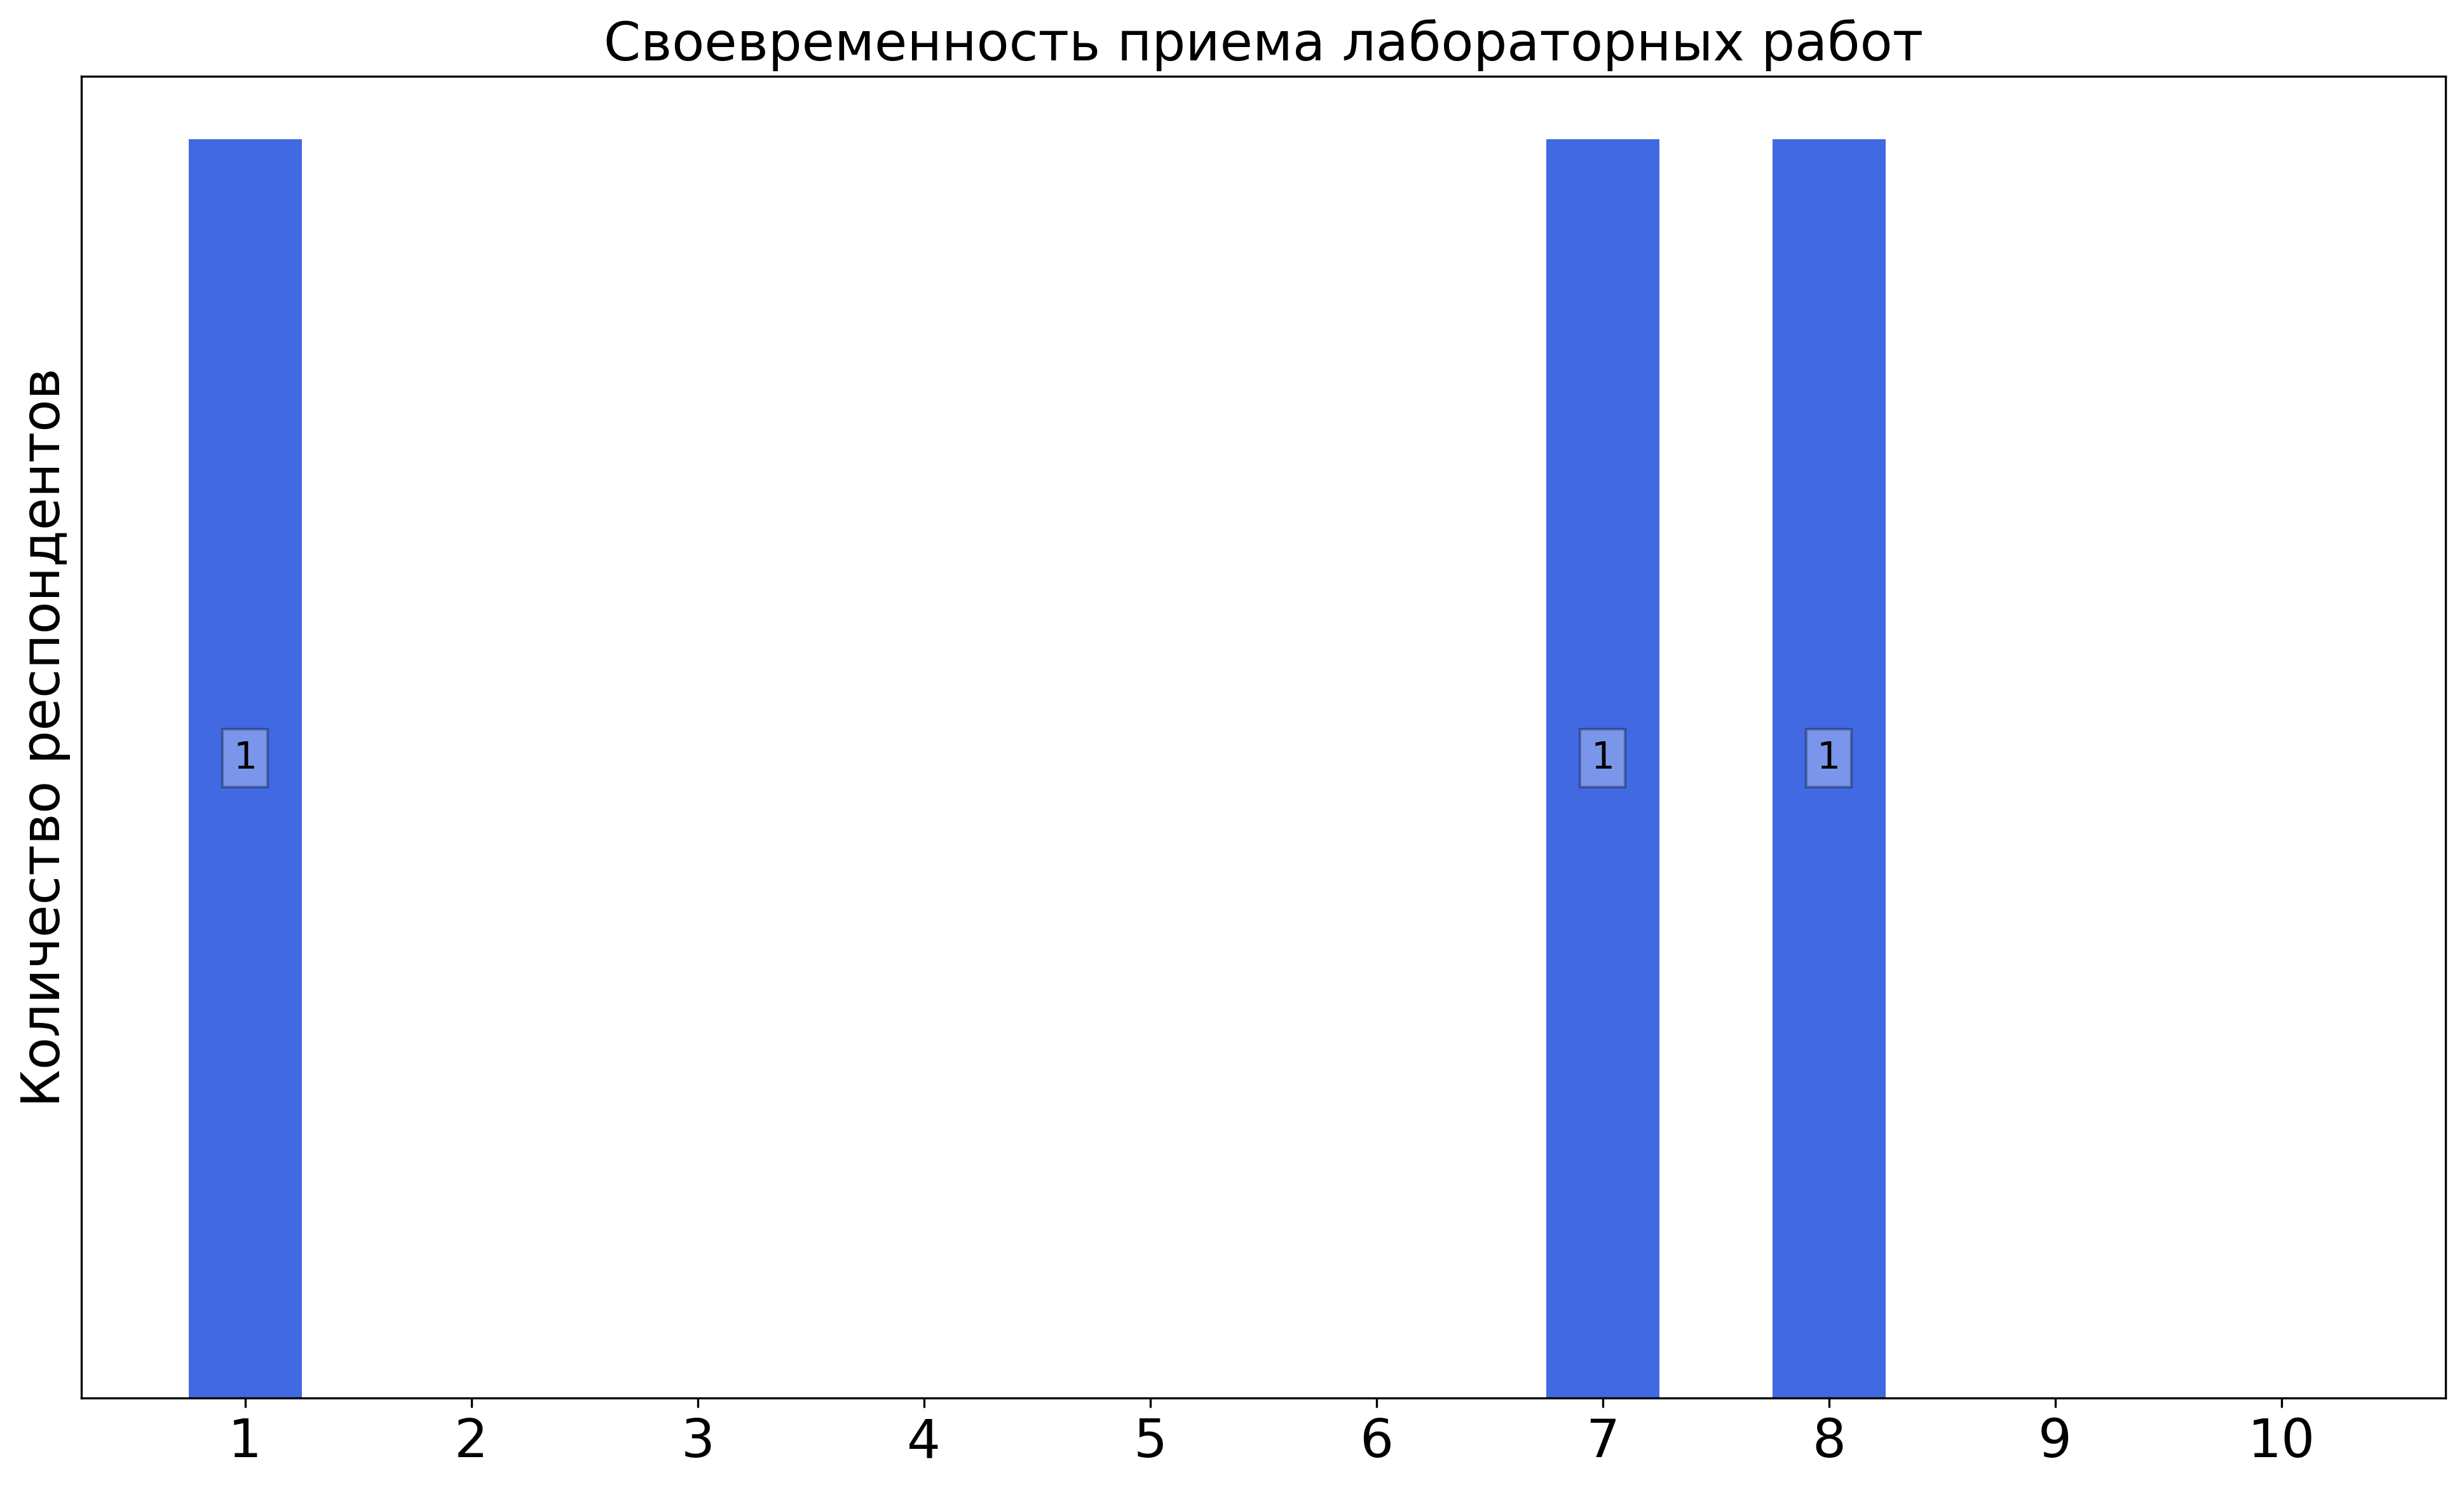
\includegraphics[width=\textwidth]{images/2 course/Радиотехнические цепи и сигналы/labniks-marks-Арумов Г.П.-2.png}
			\end{subfigure}
			\begin{subfigure}[b]{0.45\textwidth}
				\centering
				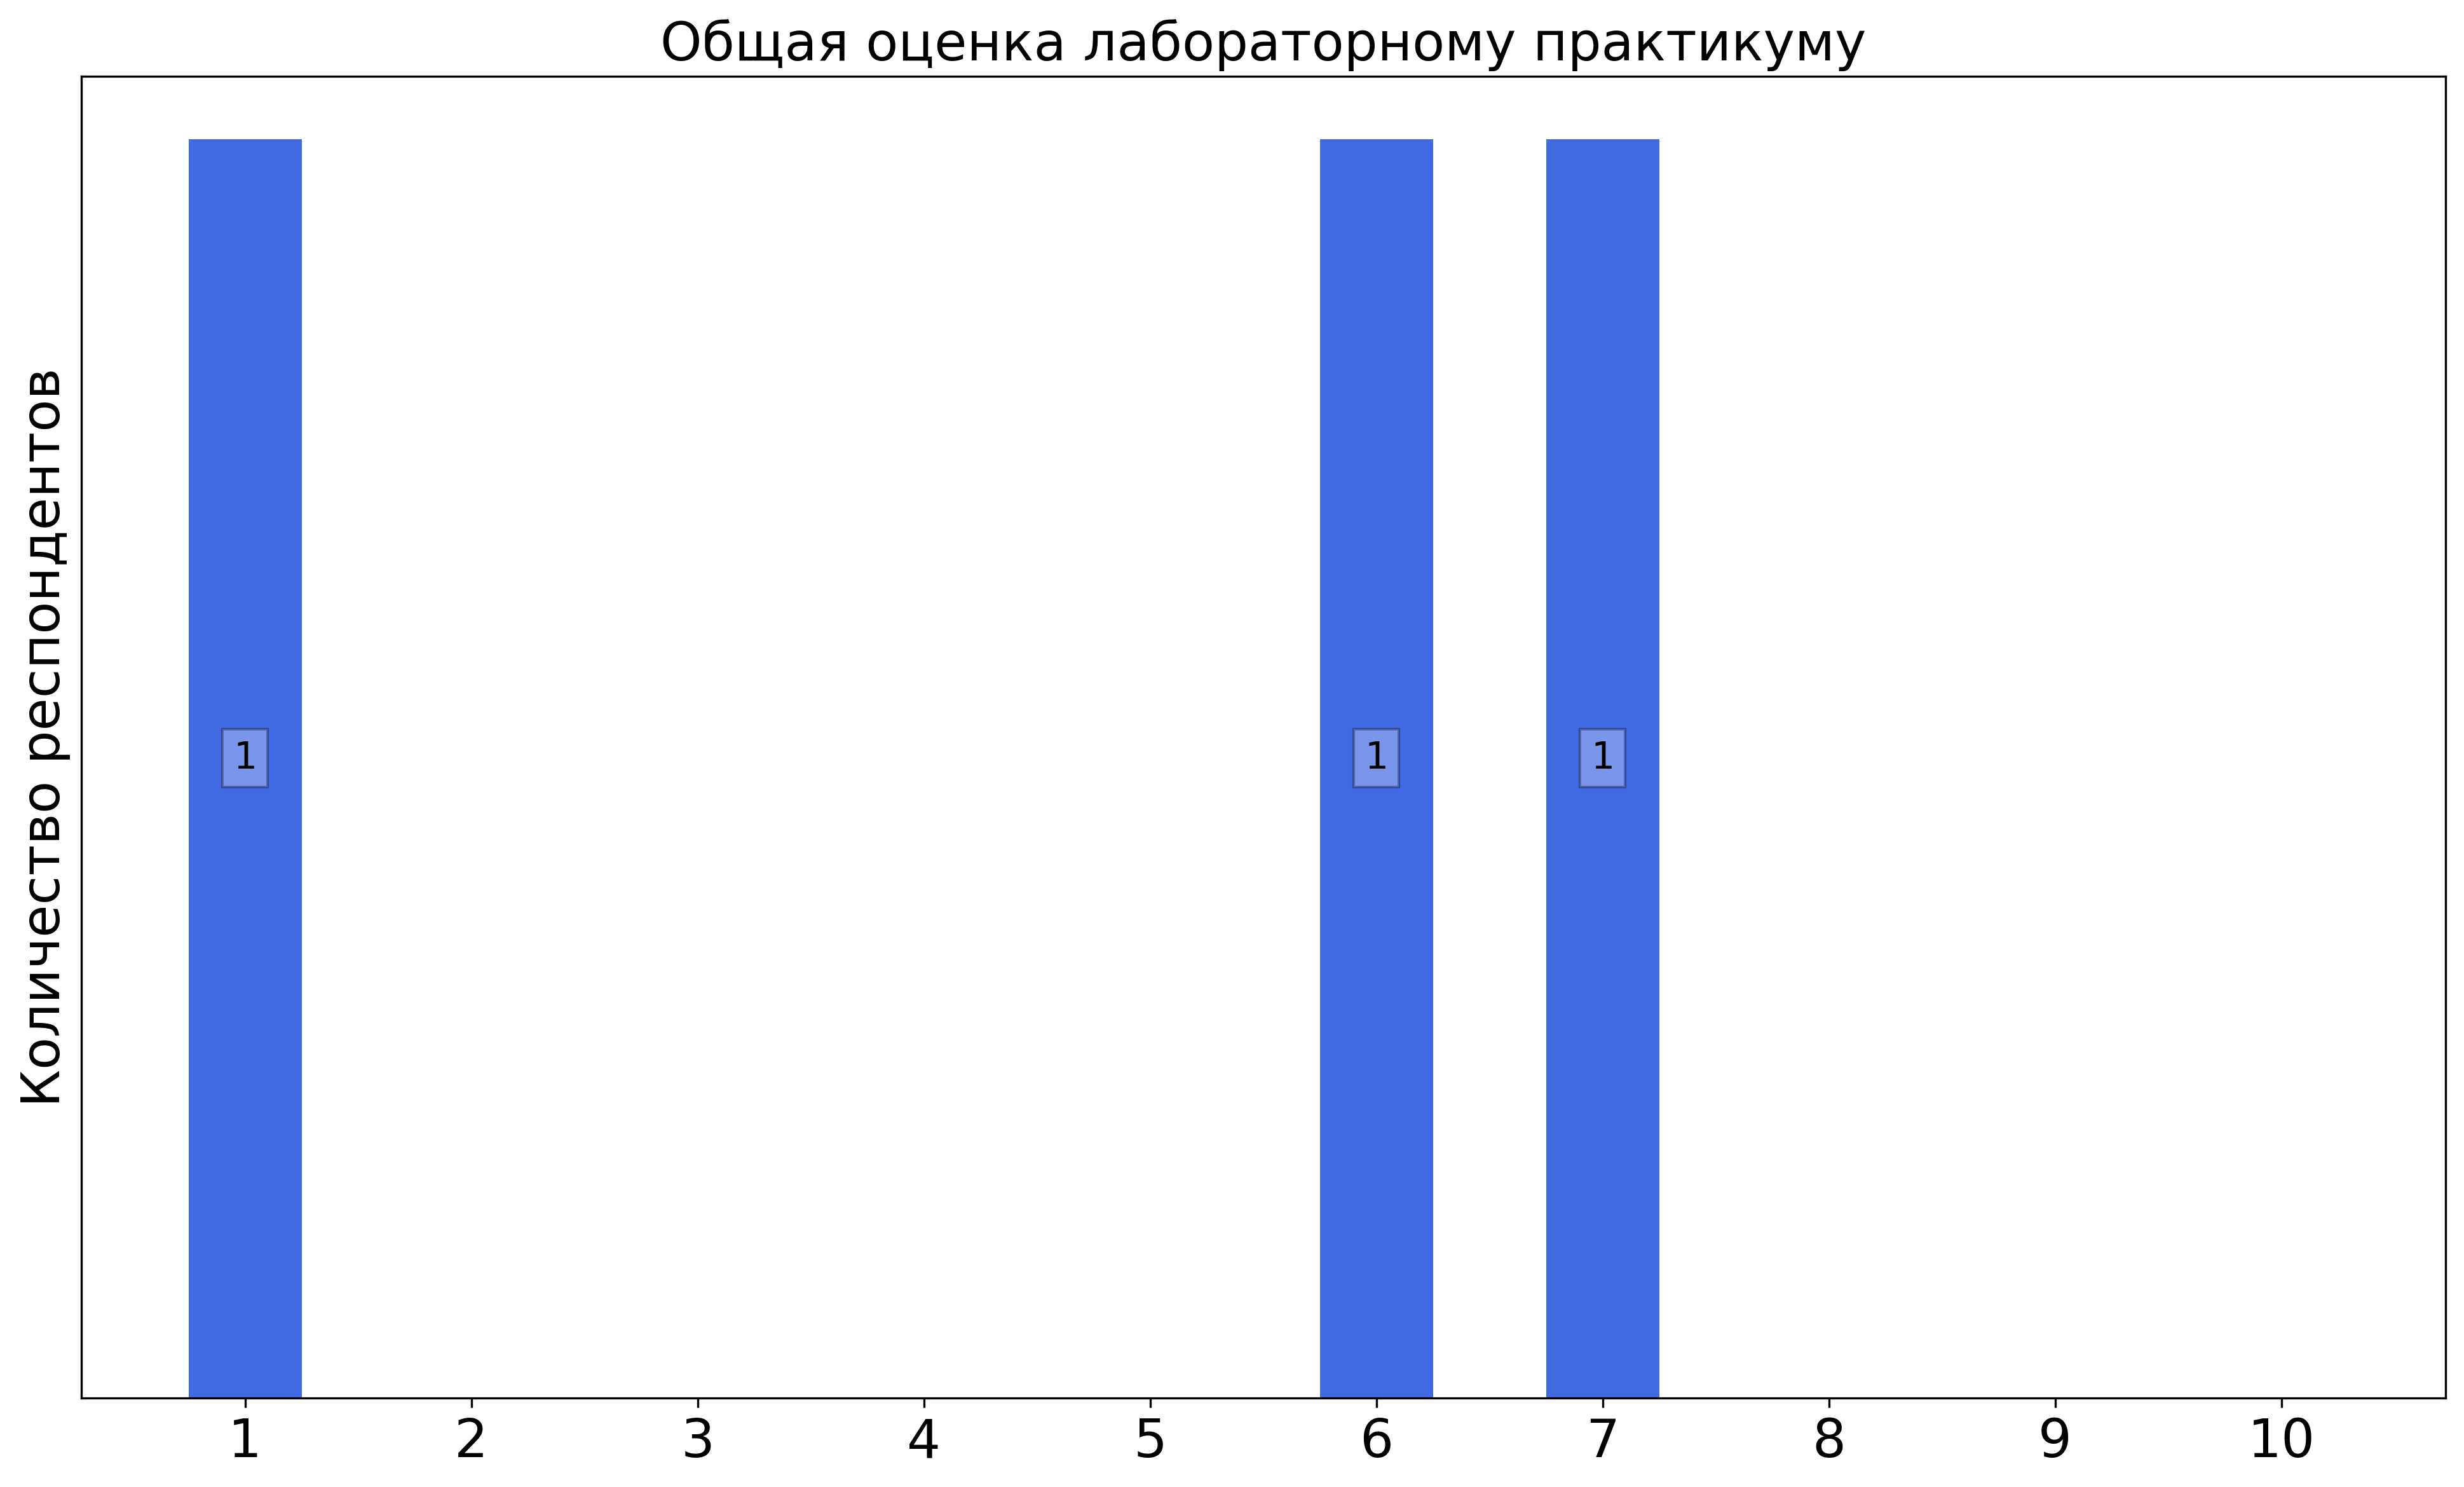
\includegraphics[width=\textwidth]{images/2 course/Радиотехнические цепи и сигналы/labniks-marks-Арумов Г.П.-3.png}
			\end{subfigure}	
			\caption{Оценки респондентов о качестве преподавания лабораторных работ}
		\end{figure}


    \subsubsection{Отзыв студентов о лабораторных работах. Преподаватель: Григорьев И.А.}
		\begin{figure}[H]
			\centering
			\begin{subfigure}[b]{0.45\textwidth}
				\centering
				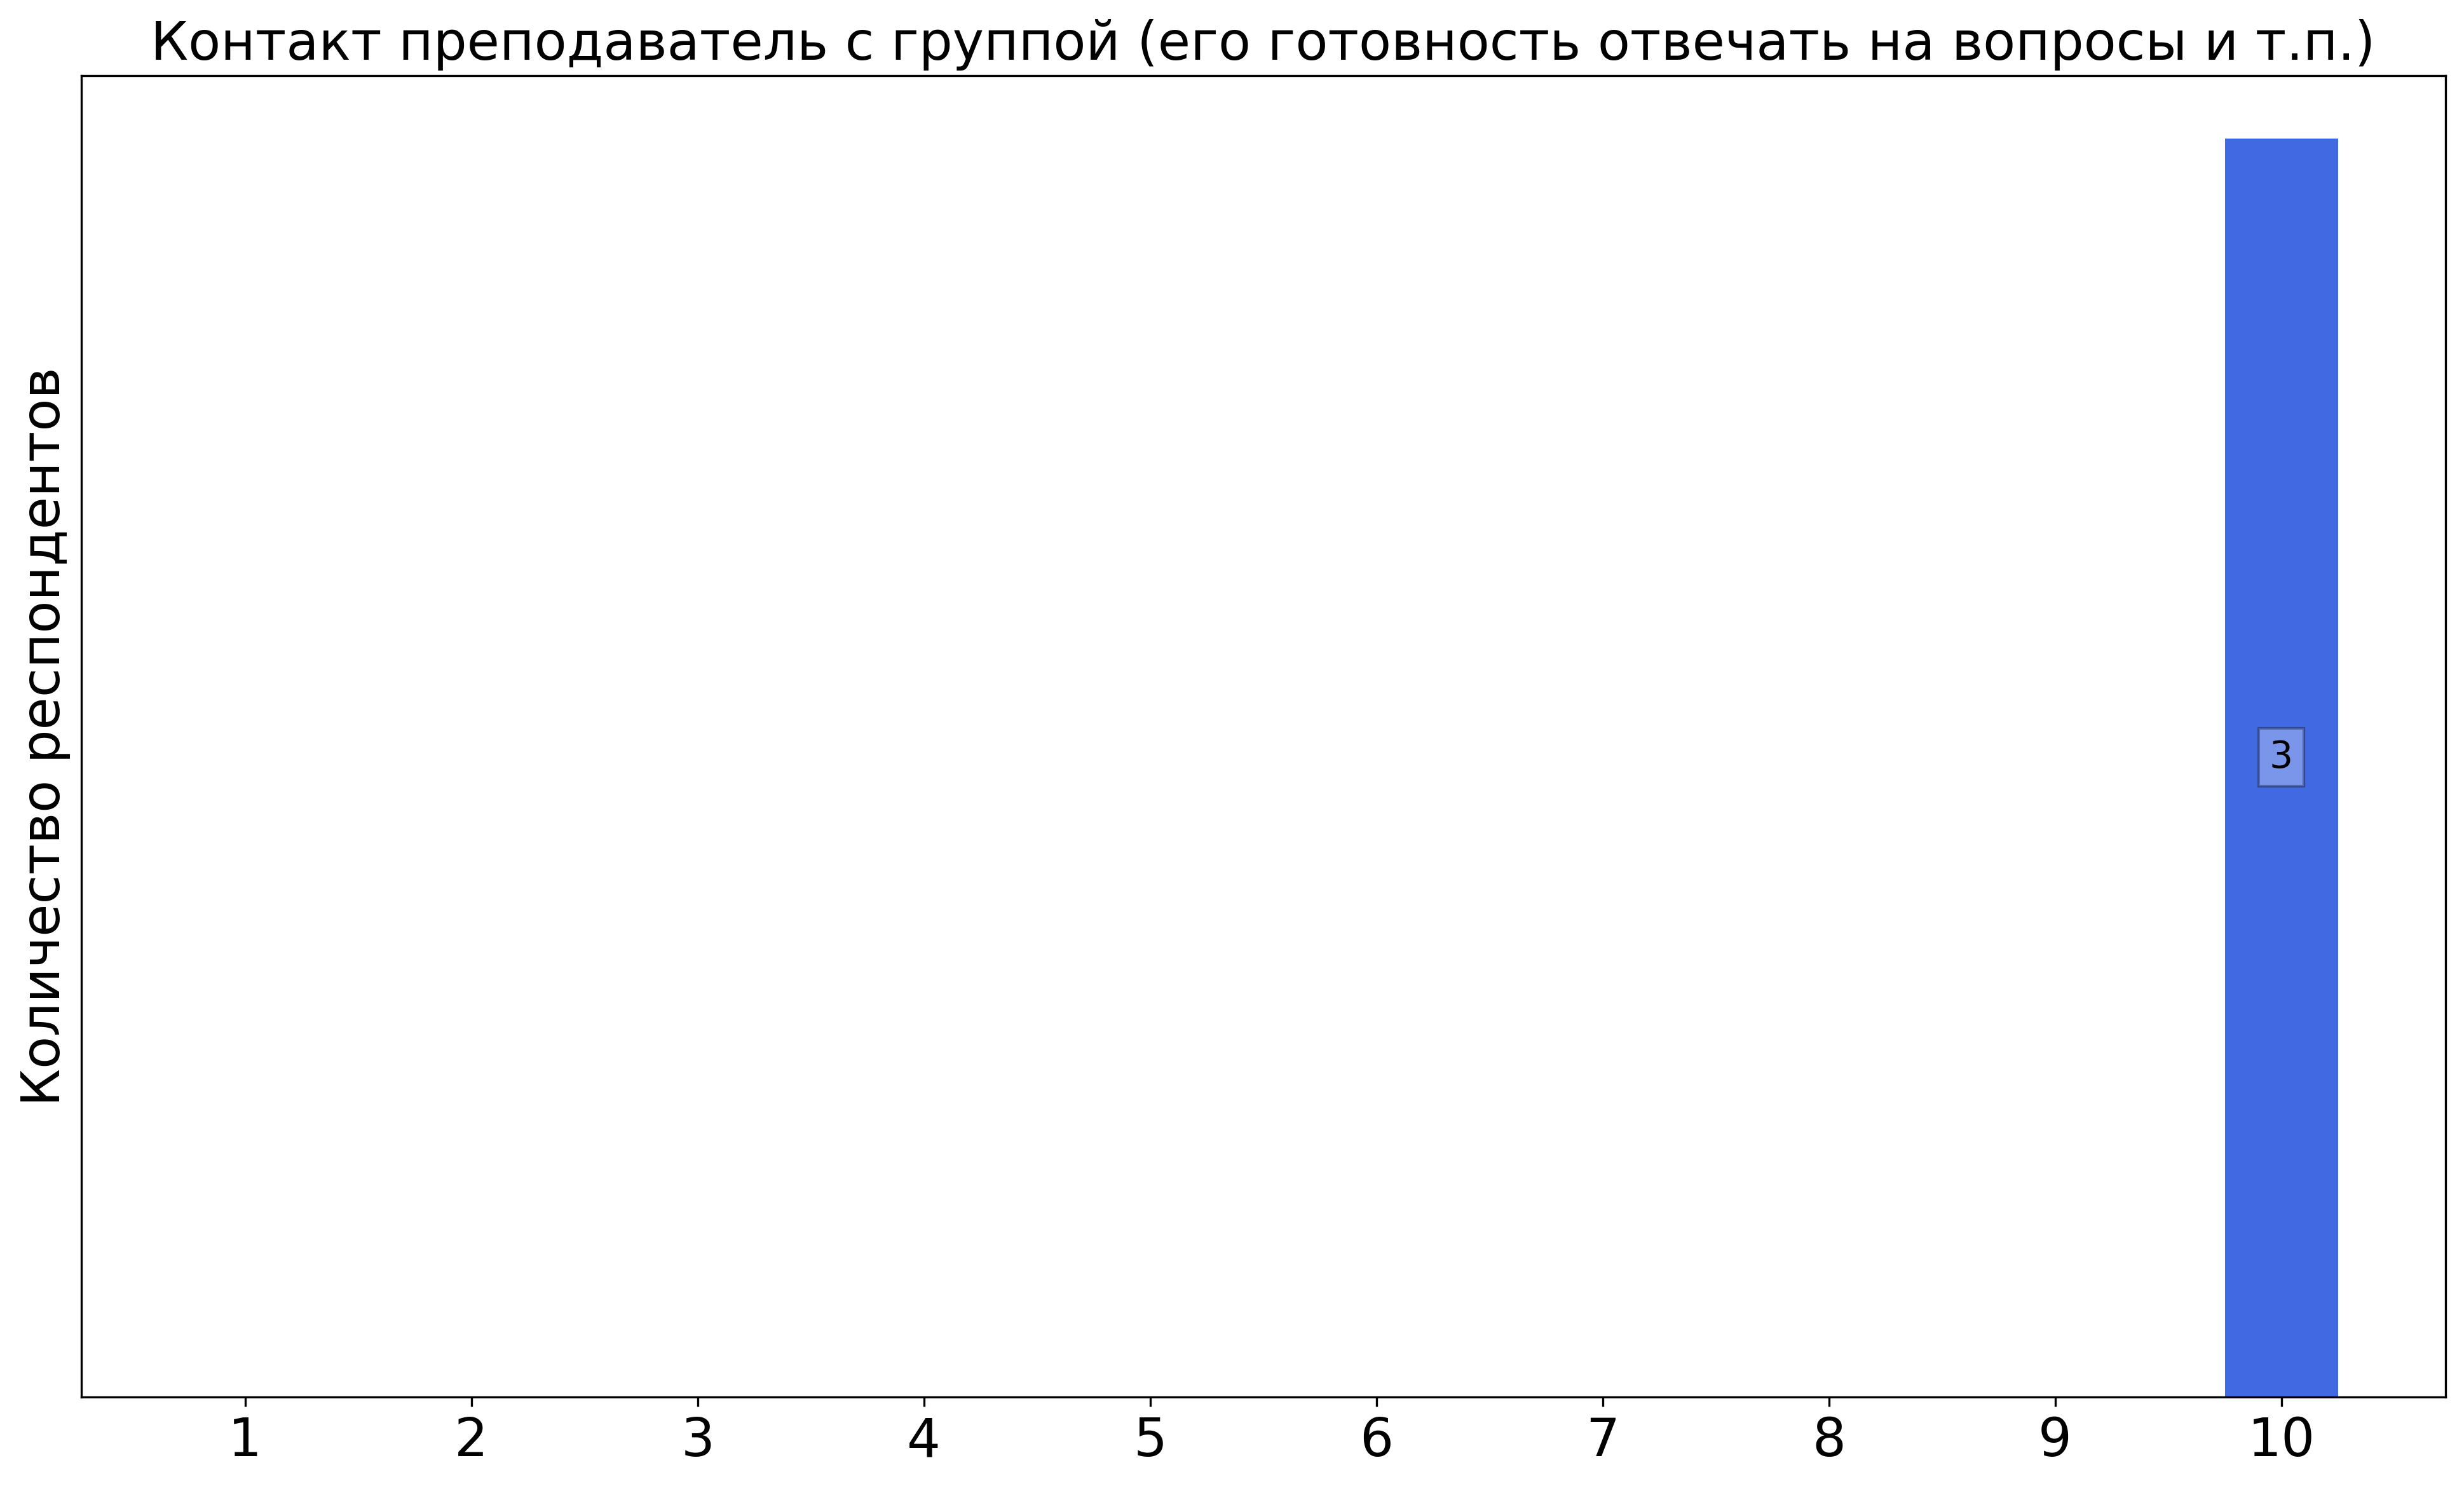
\includegraphics[width=\textwidth]{images/2 course/Радиотехнические цепи и сигналы/labniks-marks-Григорьев И.А.-0.png}
			\end{subfigure}
			\begin{subfigure}[b]{0.45\textwidth}
				\centering
				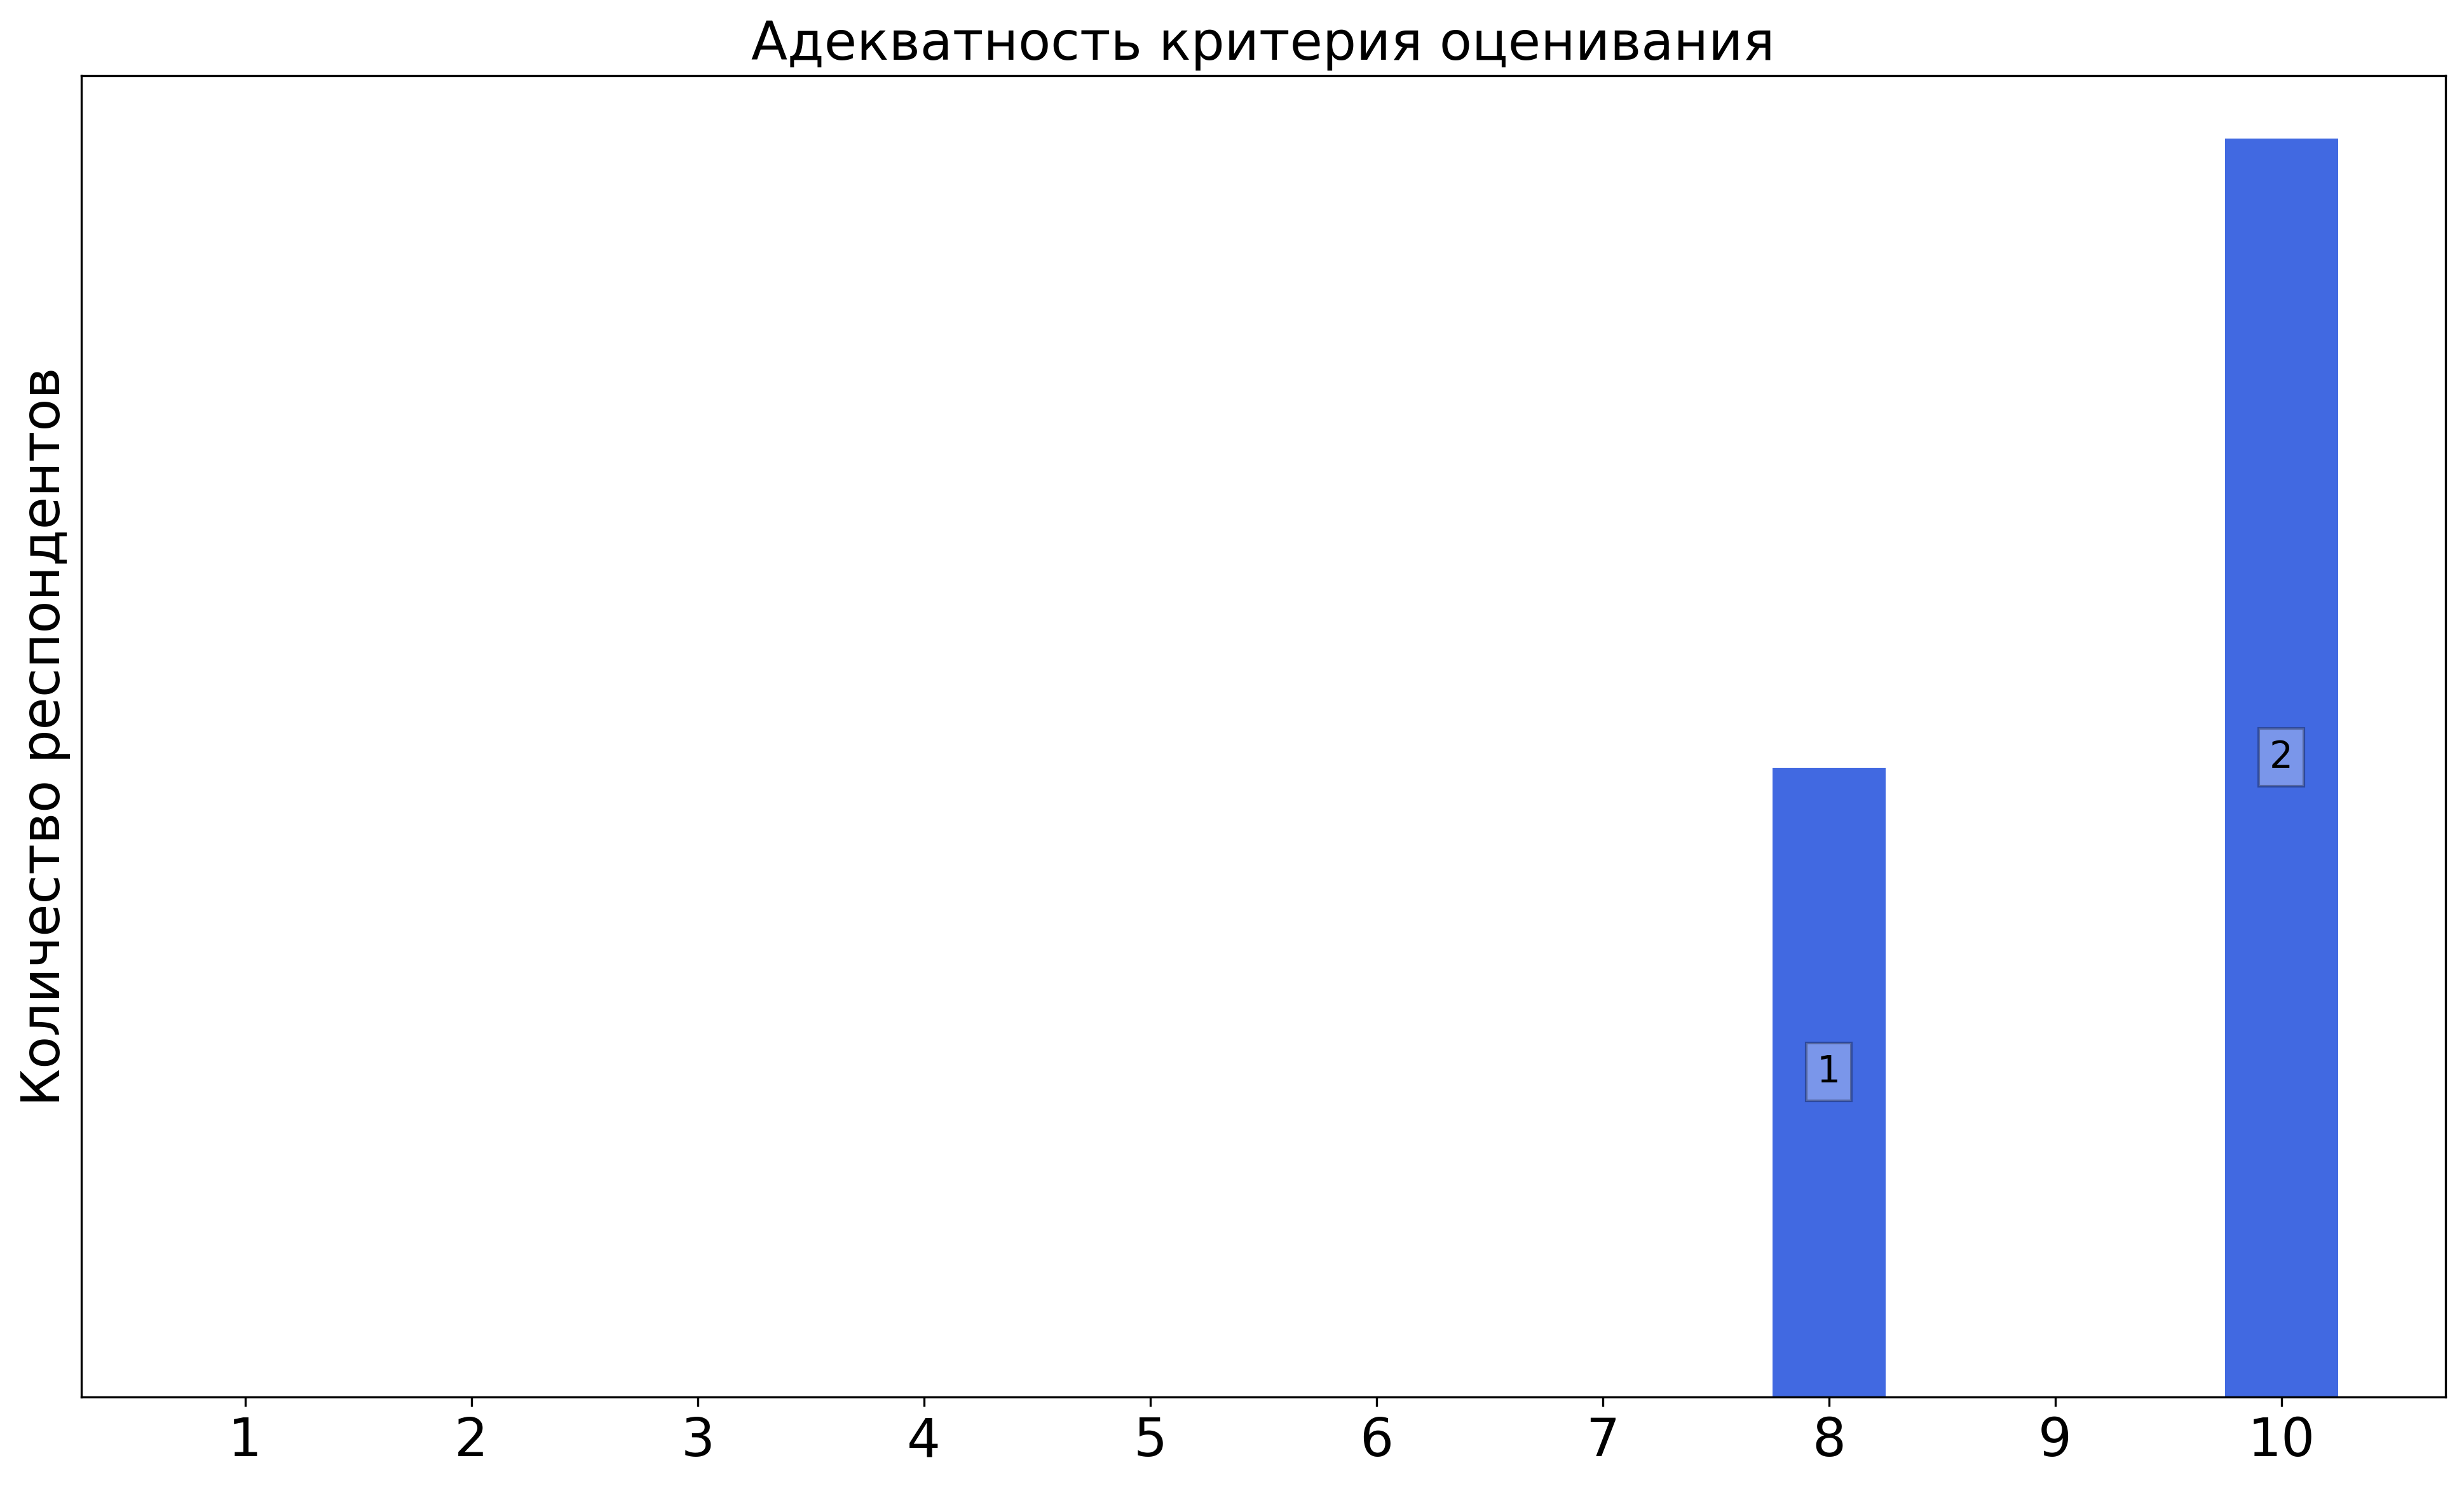
\includegraphics[width=\textwidth]{images/2 course/Радиотехнические цепи и сигналы/labniks-marks-Григорьев И.А.-1.png}
			\end{subfigure}
			\begin{subfigure}[b]{0.45\textwidth}
				\centering
				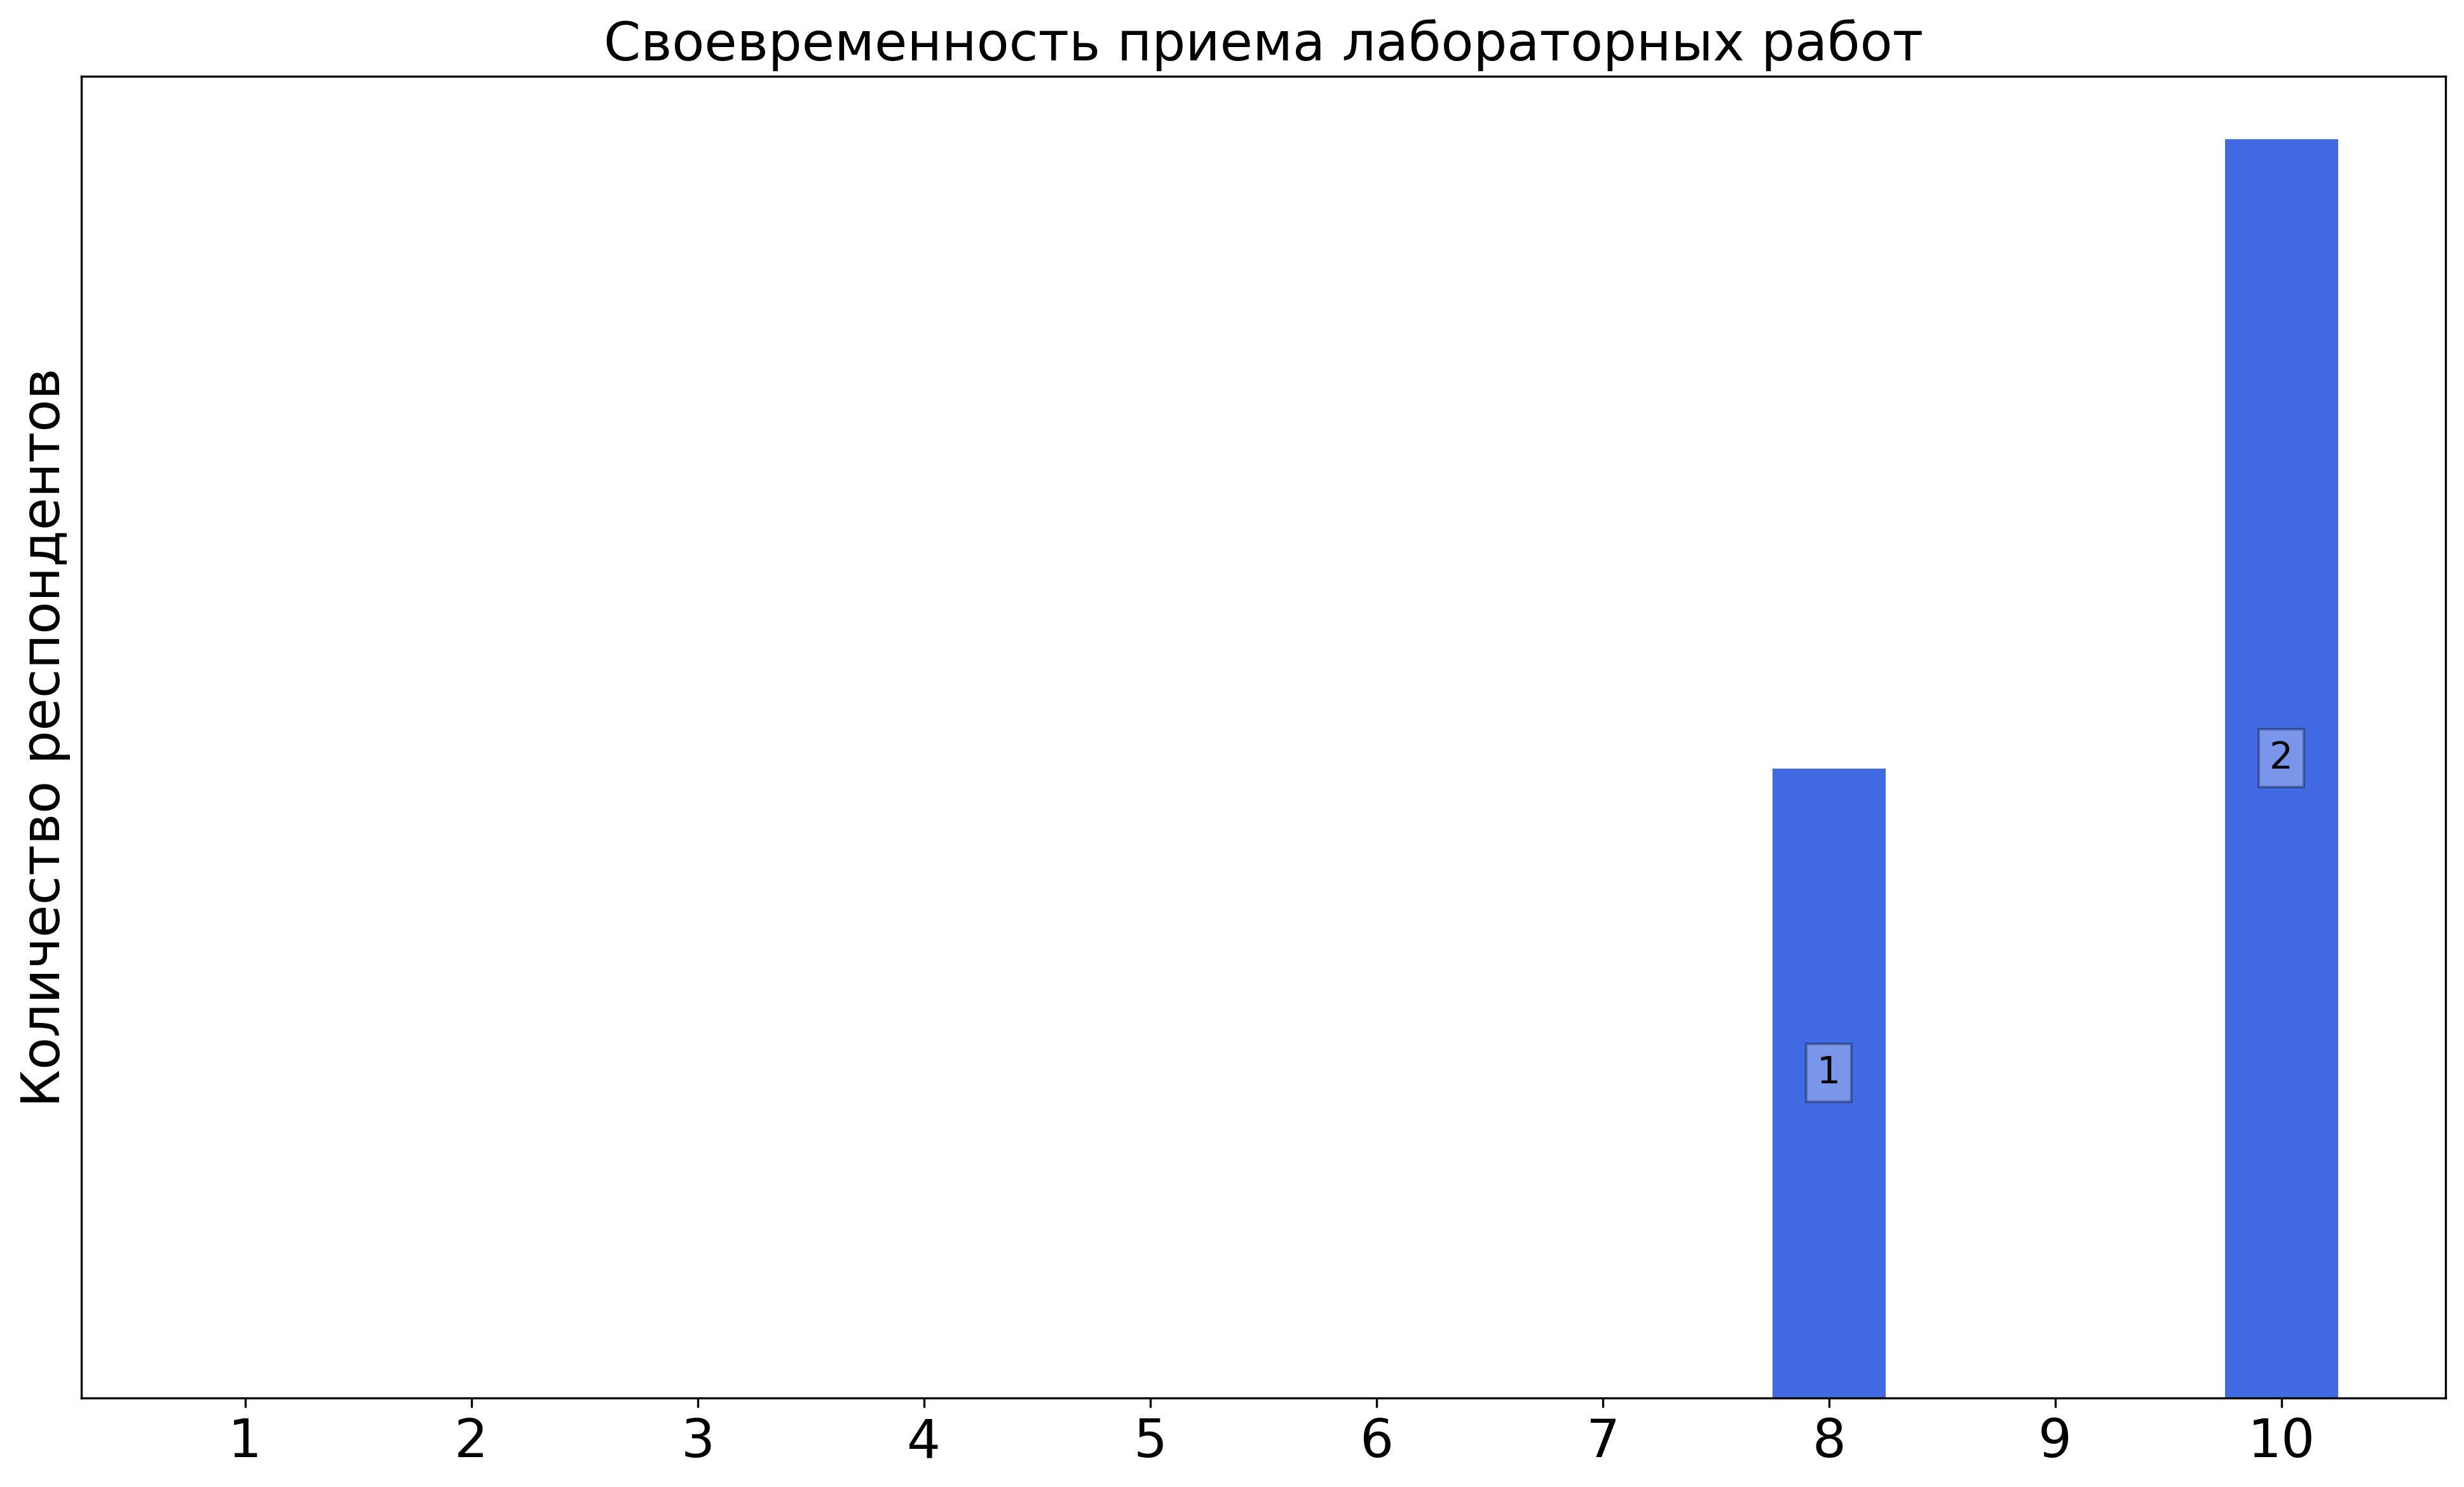
\includegraphics[width=\textwidth]{images/2 course/Радиотехнические цепи и сигналы/labniks-marks-Григорьев И.А.-2.png}
			\end{subfigure}
			\begin{subfigure}[b]{0.45\textwidth}
				\centering
				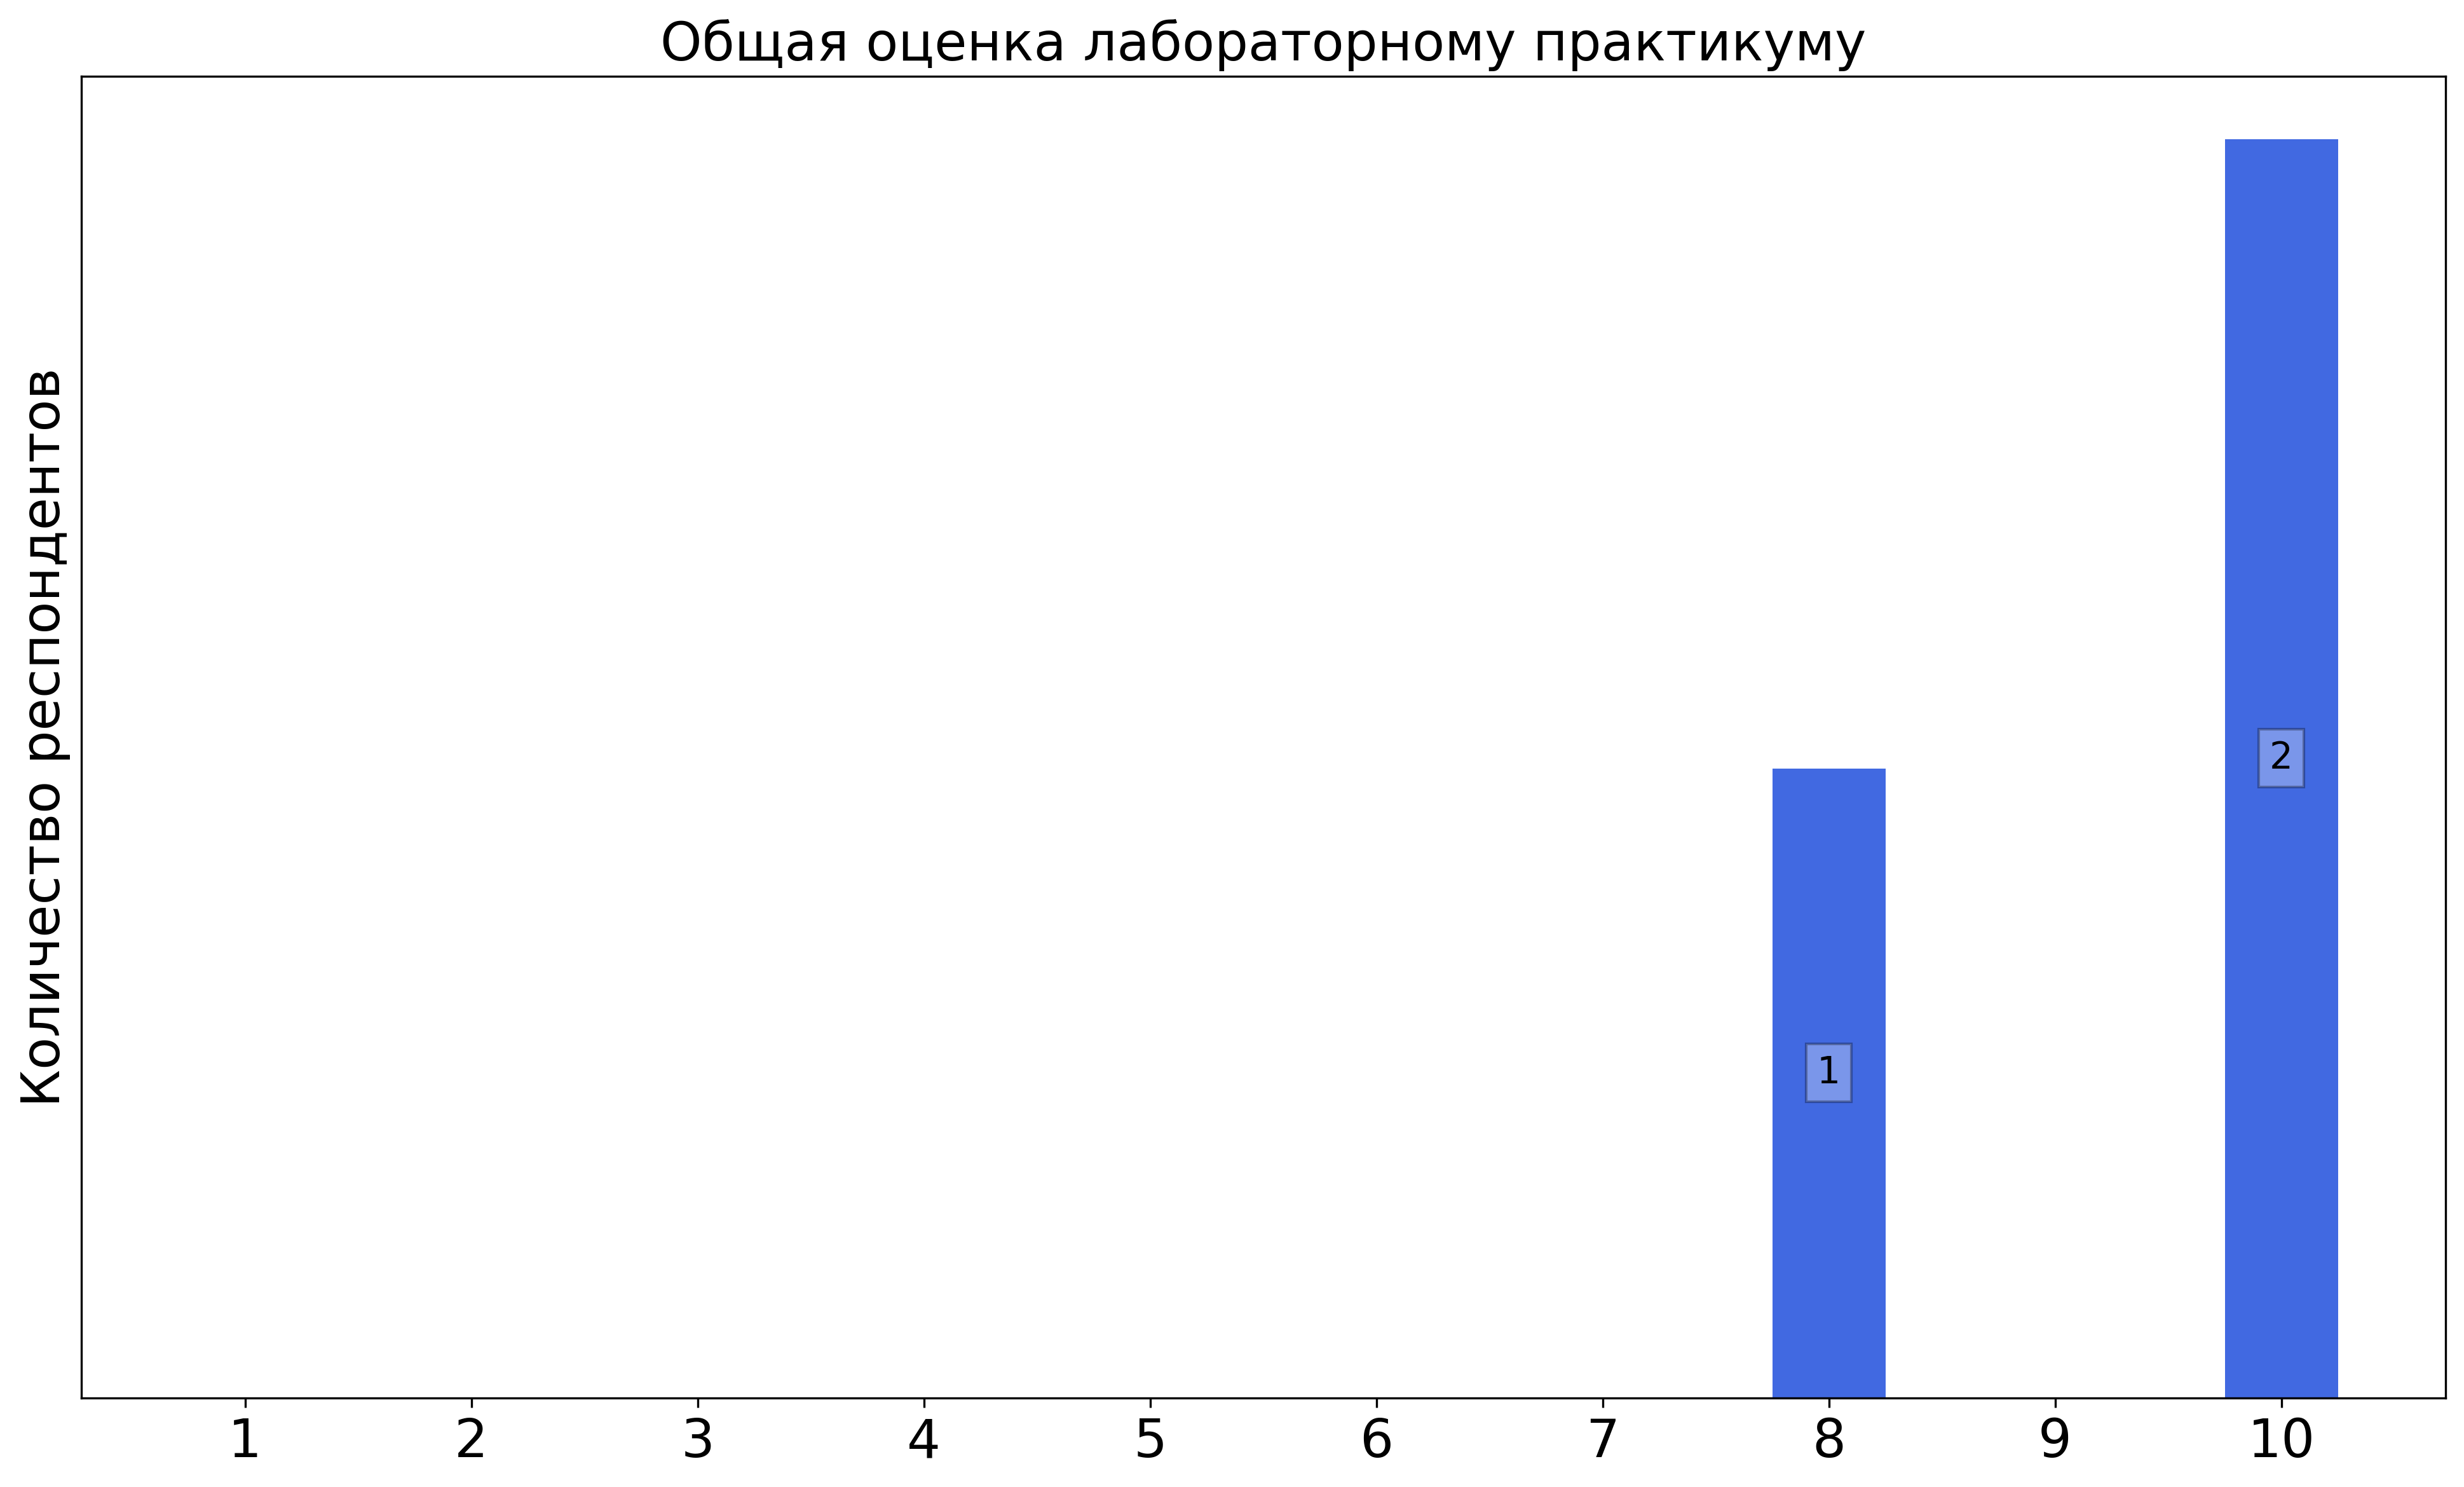
\includegraphics[width=\textwidth]{images/2 course/Радиотехнические цепи и сигналы/labniks-marks-Григорьев И.А.-3.png}
			\end{subfigure}	
			\caption{Оценки респондентов о качестве преподавания лабораторных работ}
		\end{figure}


    
    \subsubsection{Отзыв студентов о лабораторных работах. Преподаватель: Двойнишников Д.А. }
		\begin{figure}[H]
			\centering
			\begin{subfigure}[b]{0.45\textwidth}
				\centering
				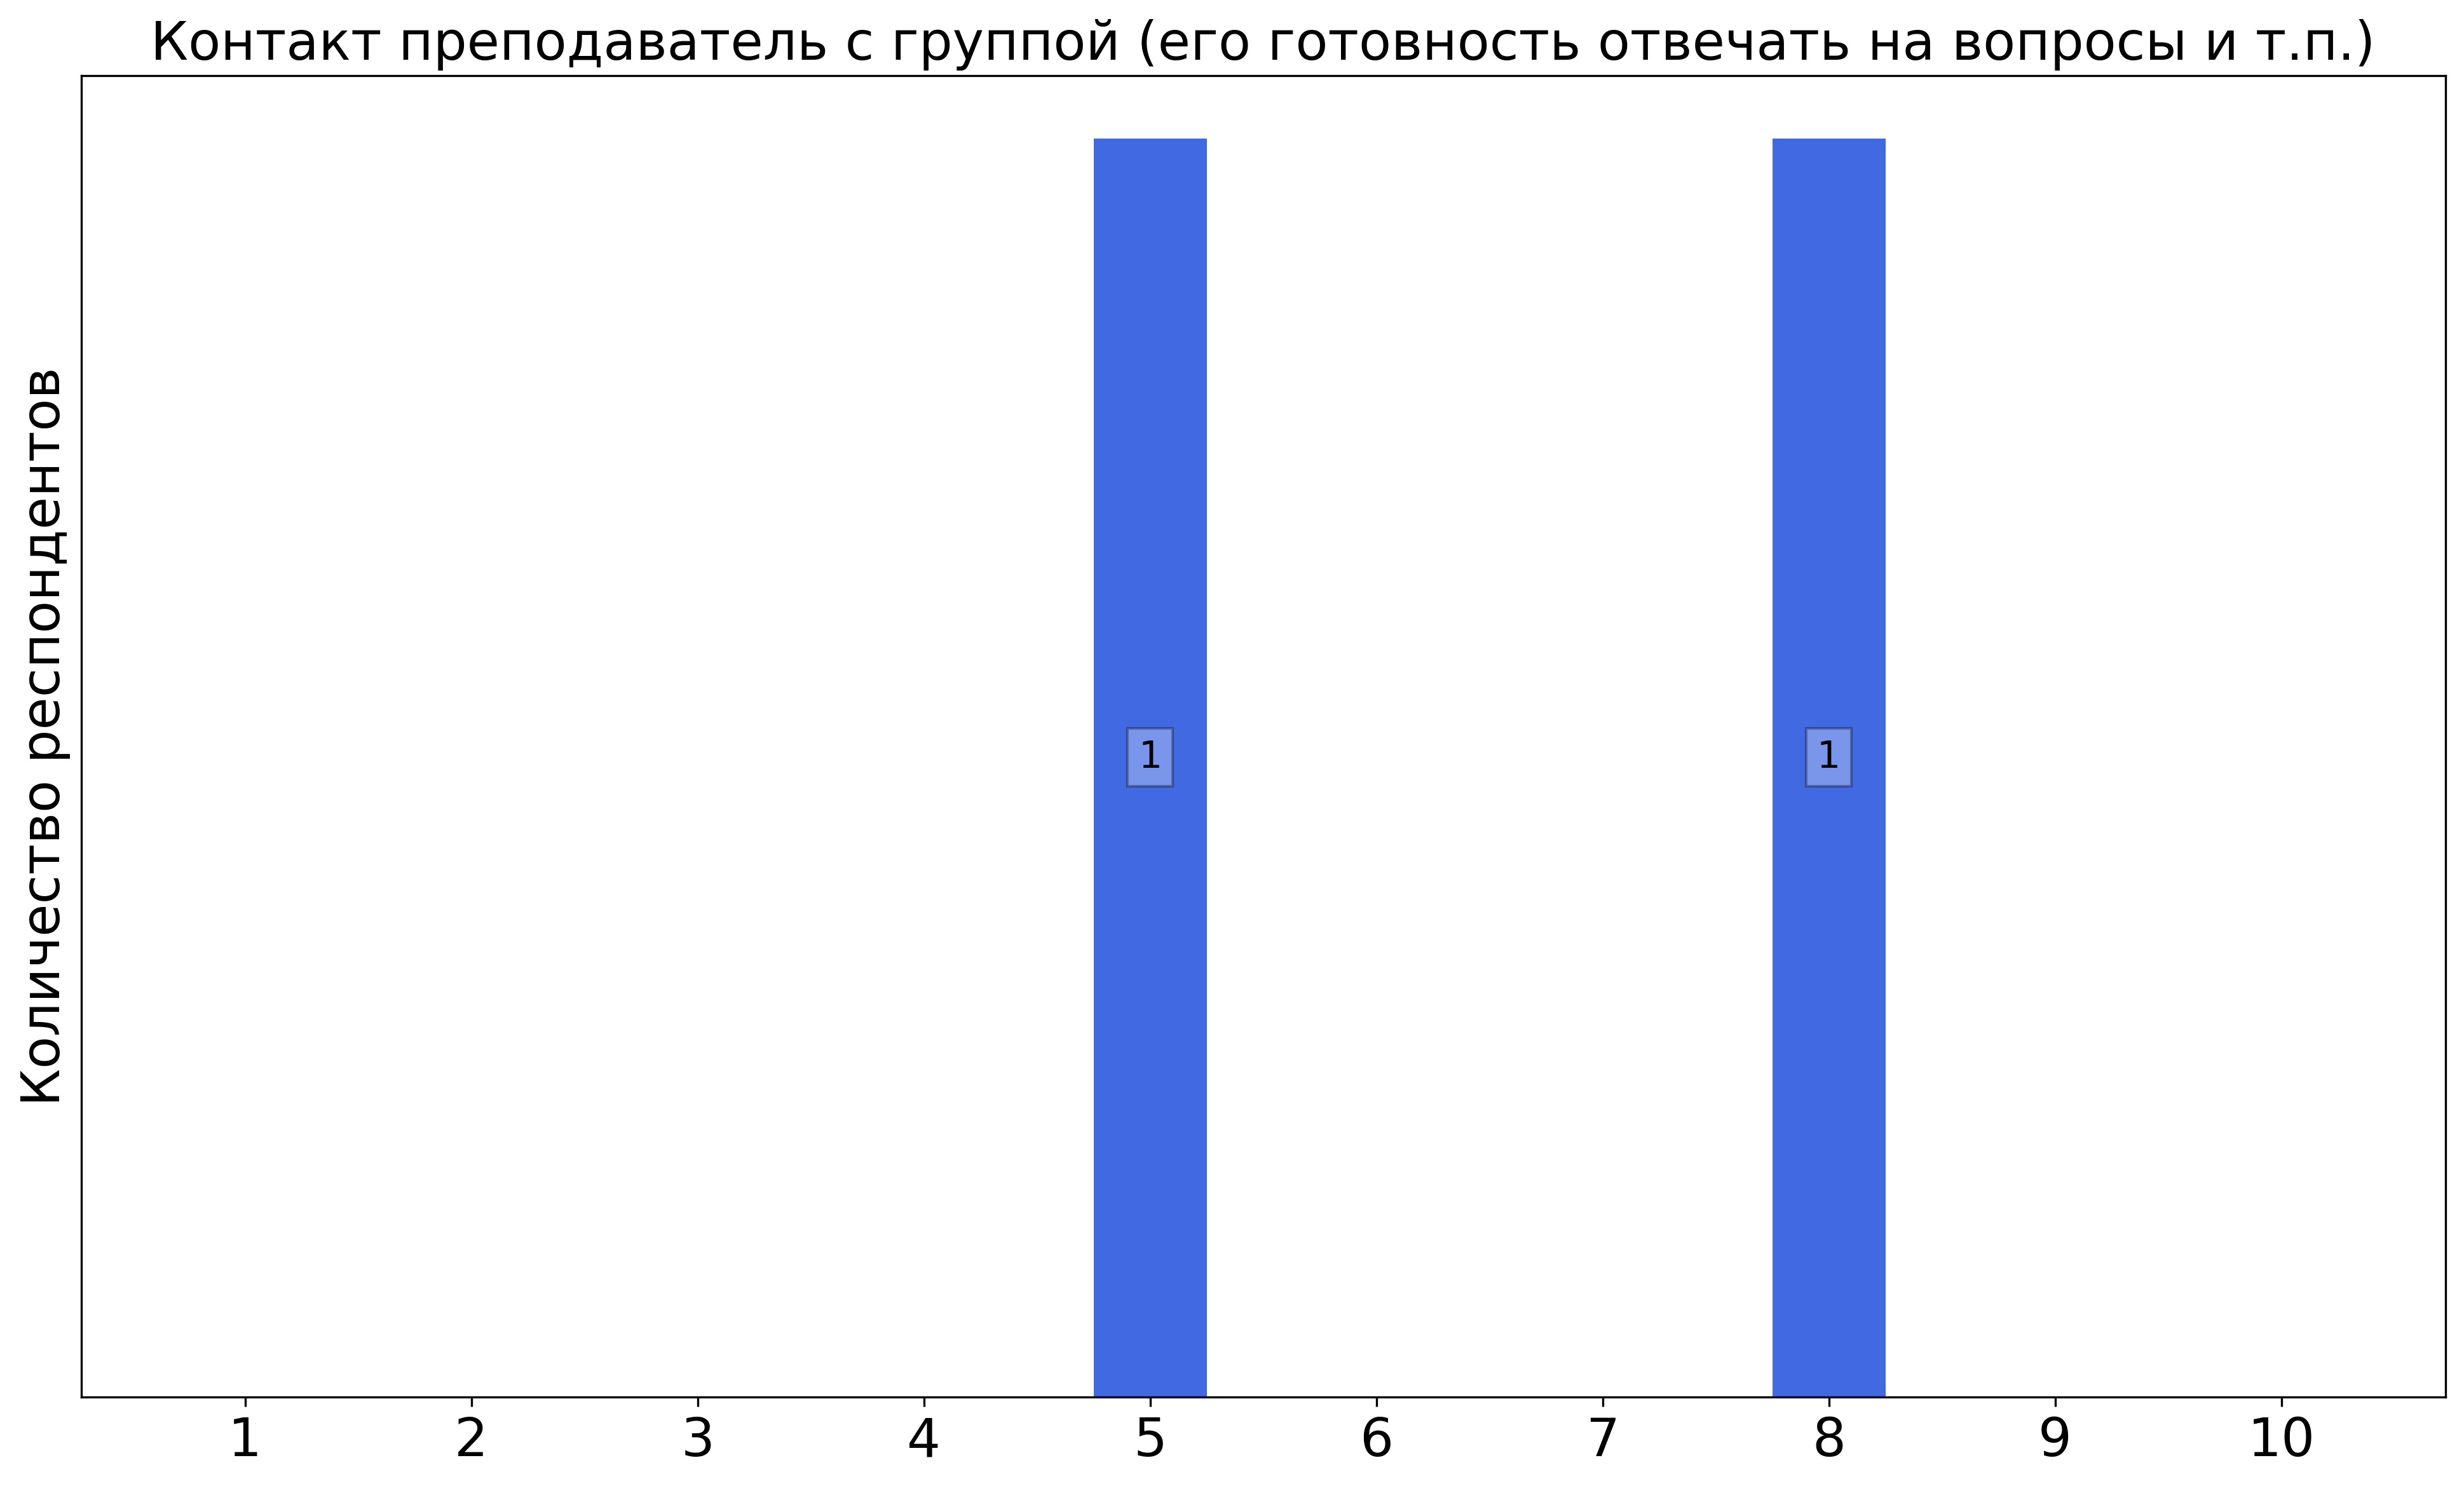
\includegraphics[width=\textwidth]{images/2 course/Радиотехнические цепи и сигналы/labniks-marks-Двойнишников Д.А. -0.png}
			\end{subfigure}
			\begin{subfigure}[b]{0.45\textwidth}
				\centering
				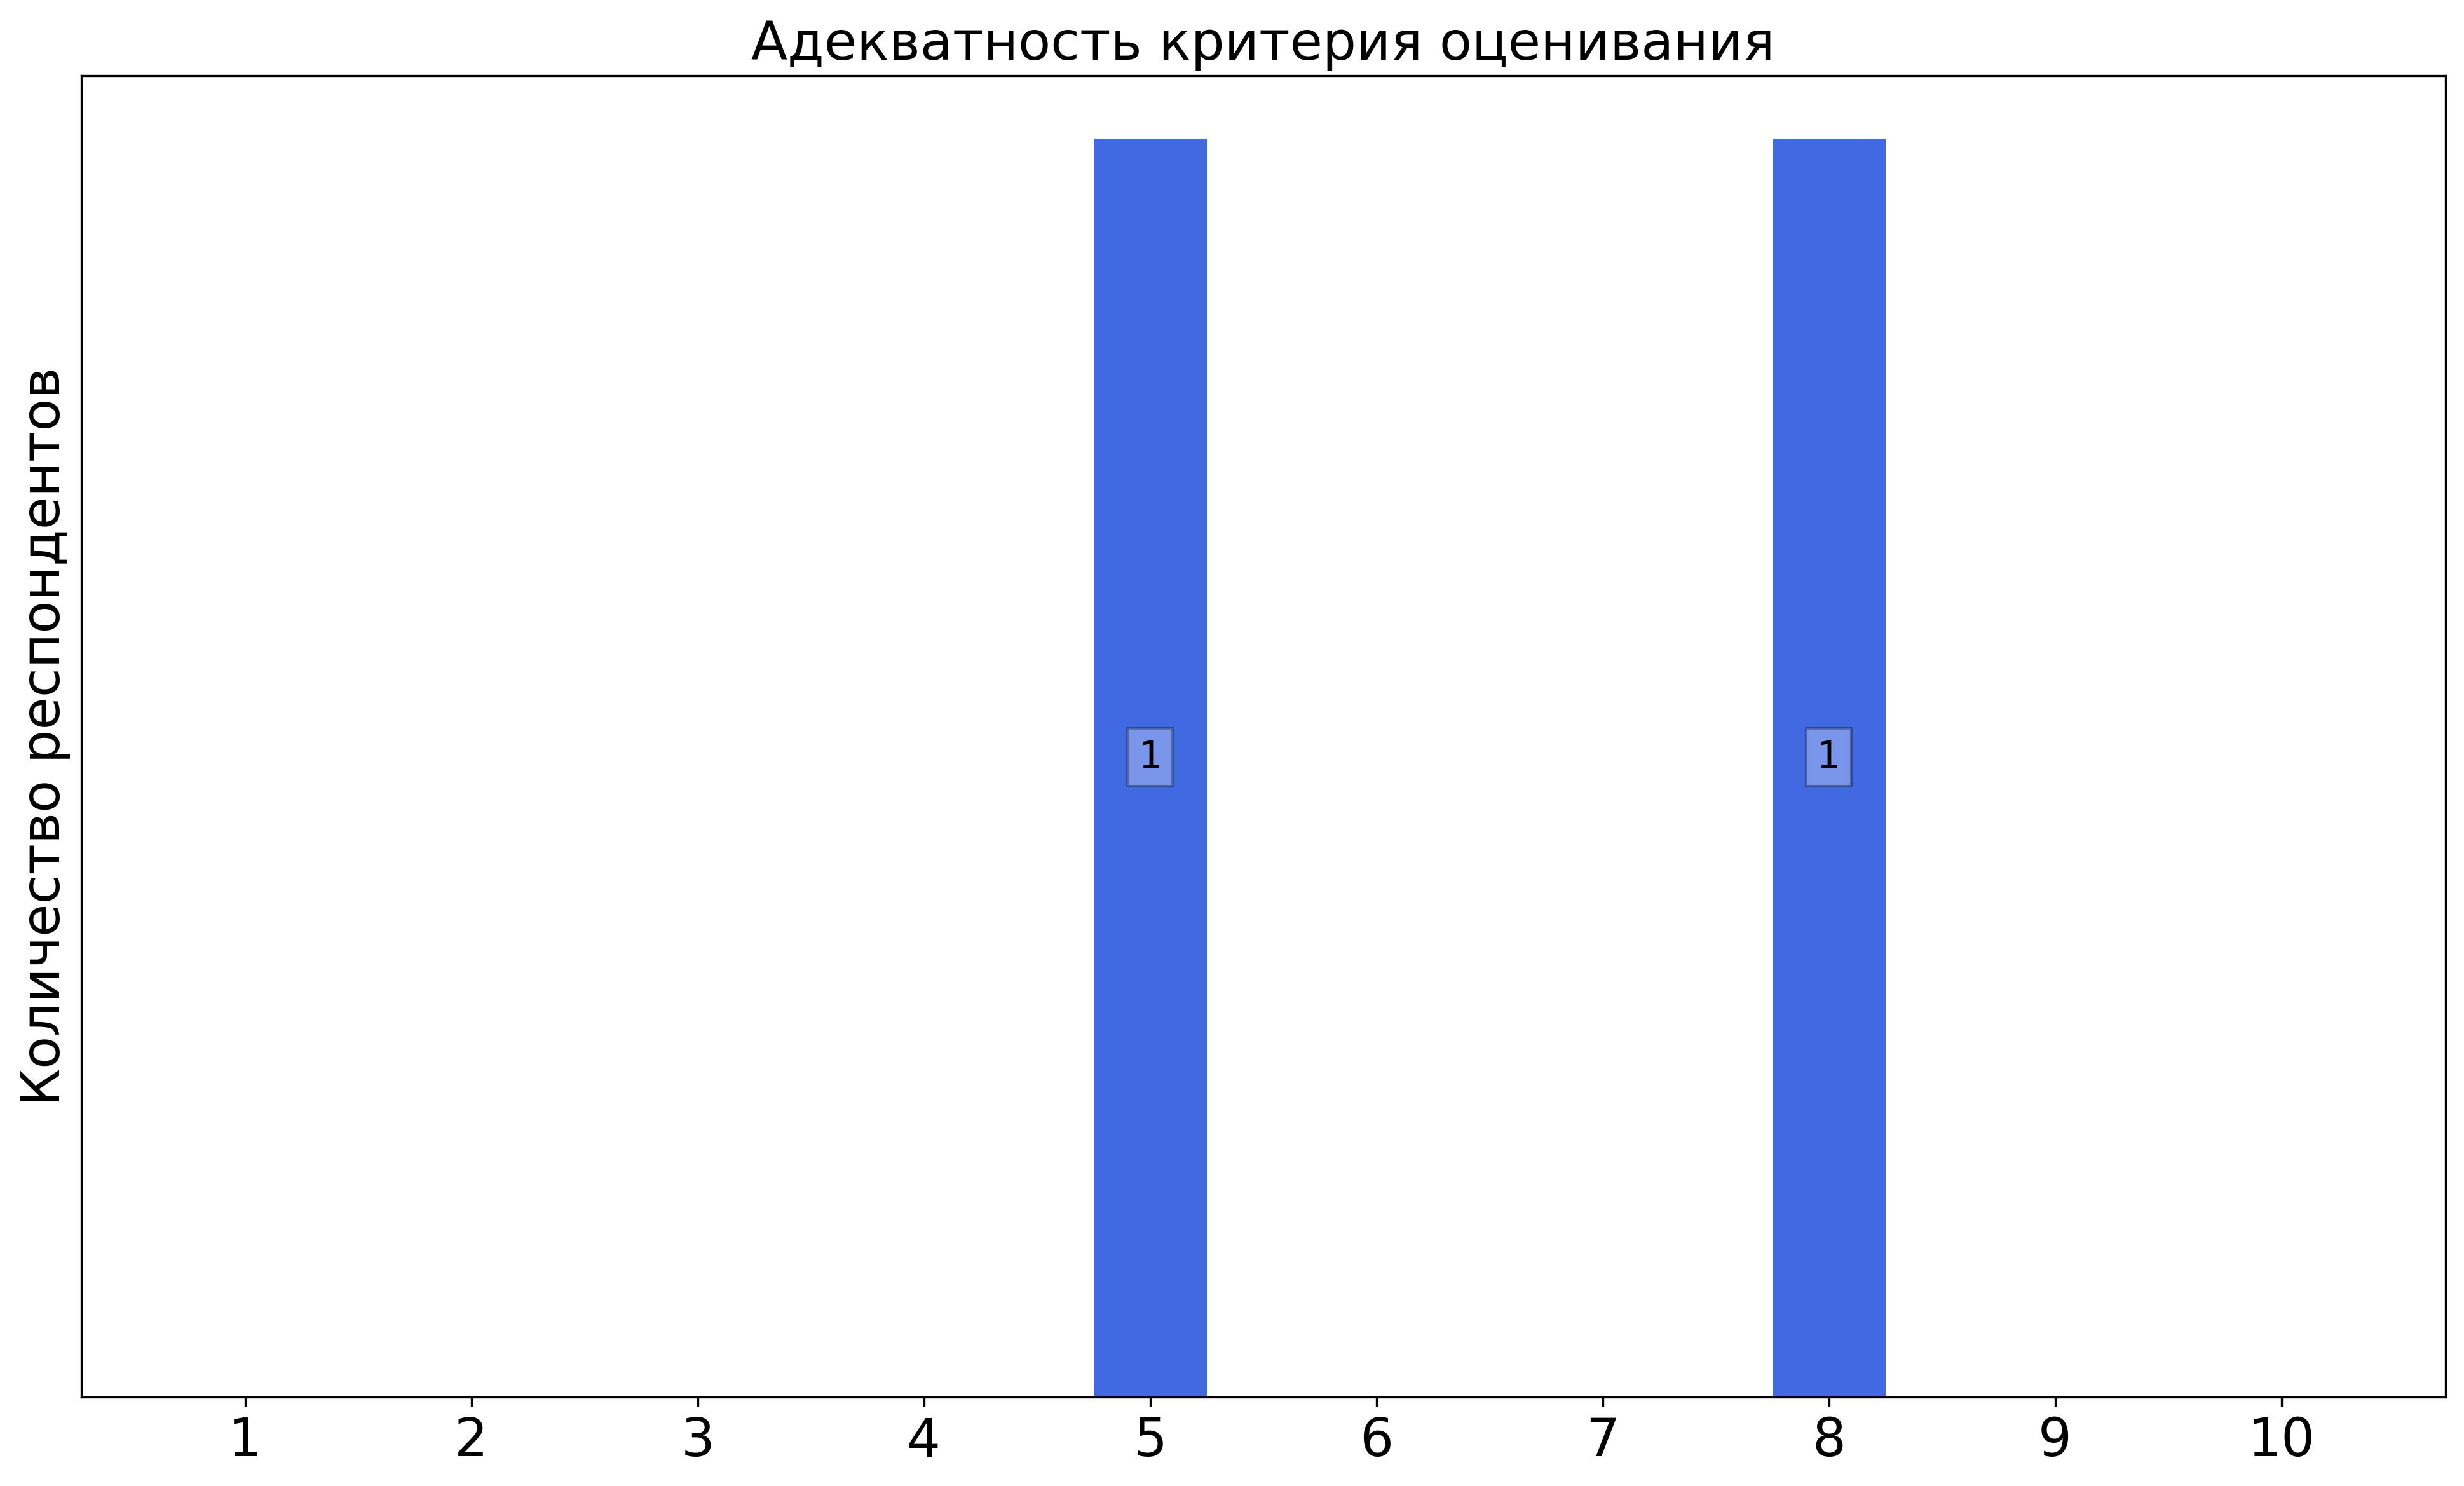
\includegraphics[width=\textwidth]{images/2 course/Радиотехнические цепи и сигналы/labniks-marks-Двойнишников Д.А. -1.png}
			\end{subfigure}
			\begin{subfigure}[b]{0.45\textwidth}
				\centering
				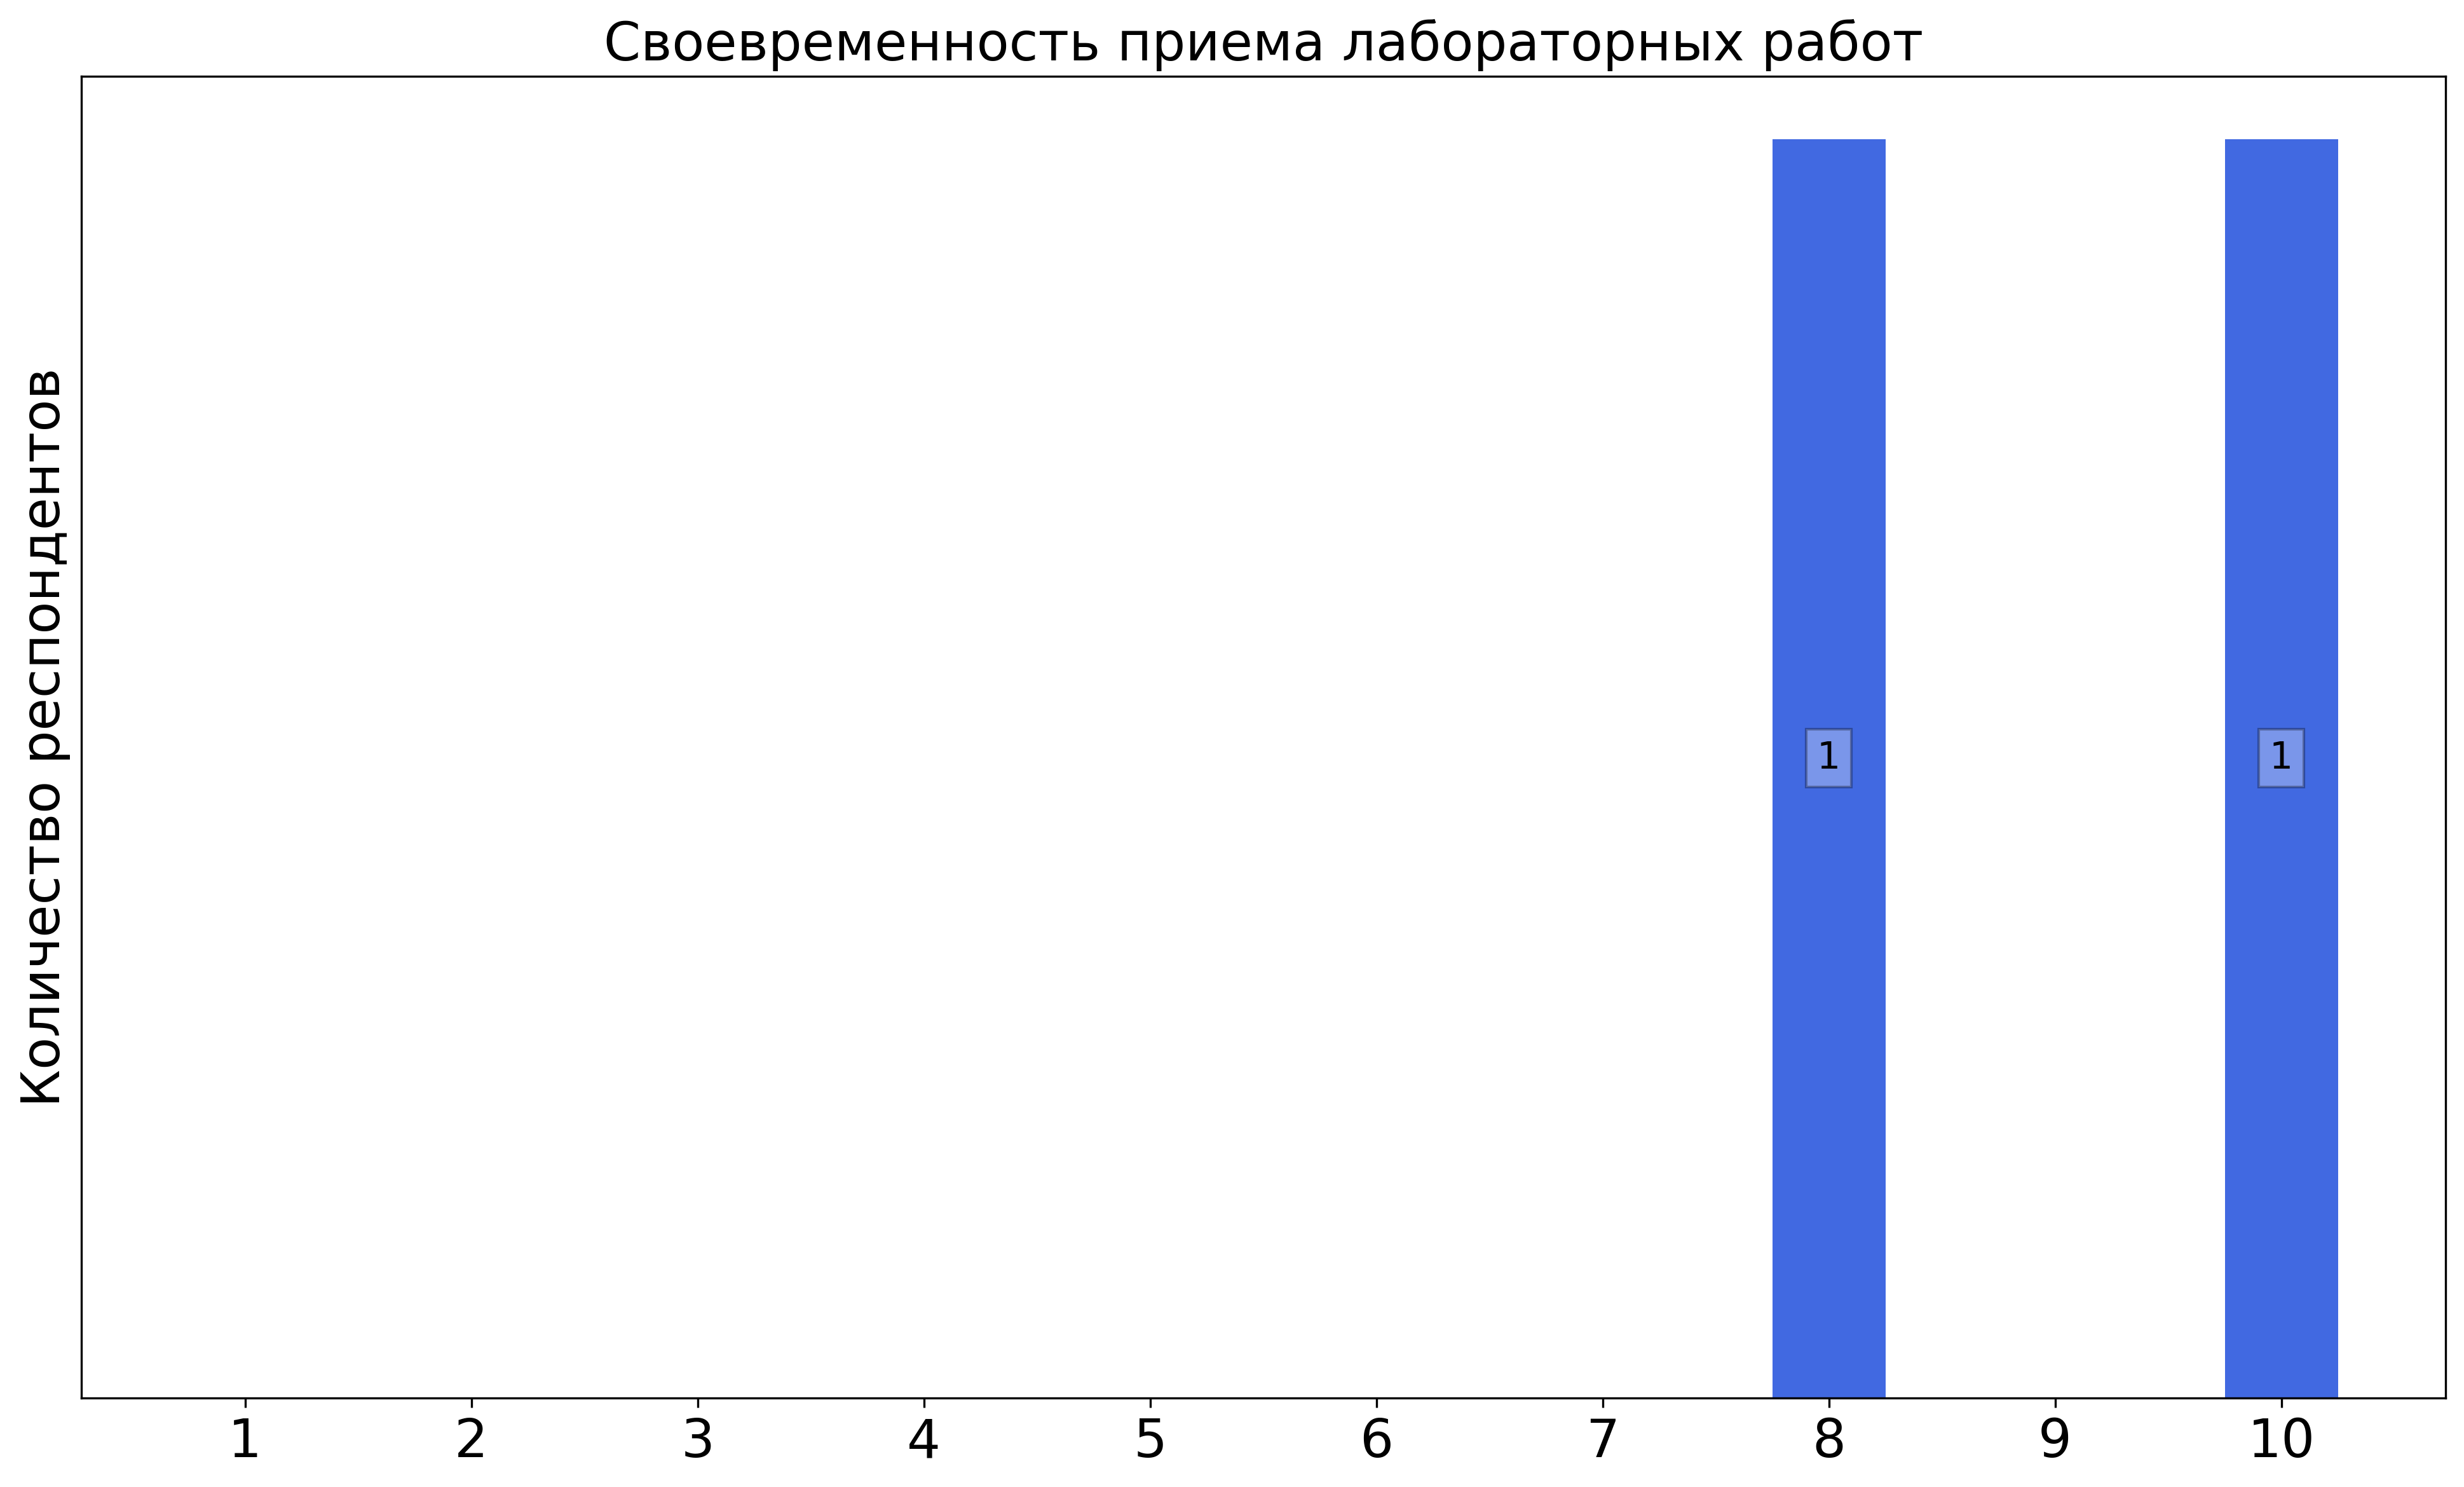
\includegraphics[width=\textwidth]{images/2 course/Радиотехнические цепи и сигналы/labniks-marks-Двойнишников Д.А. -2.png}
			\end{subfigure}
			\begin{subfigure}[b]{0.45\textwidth}
				\centering
				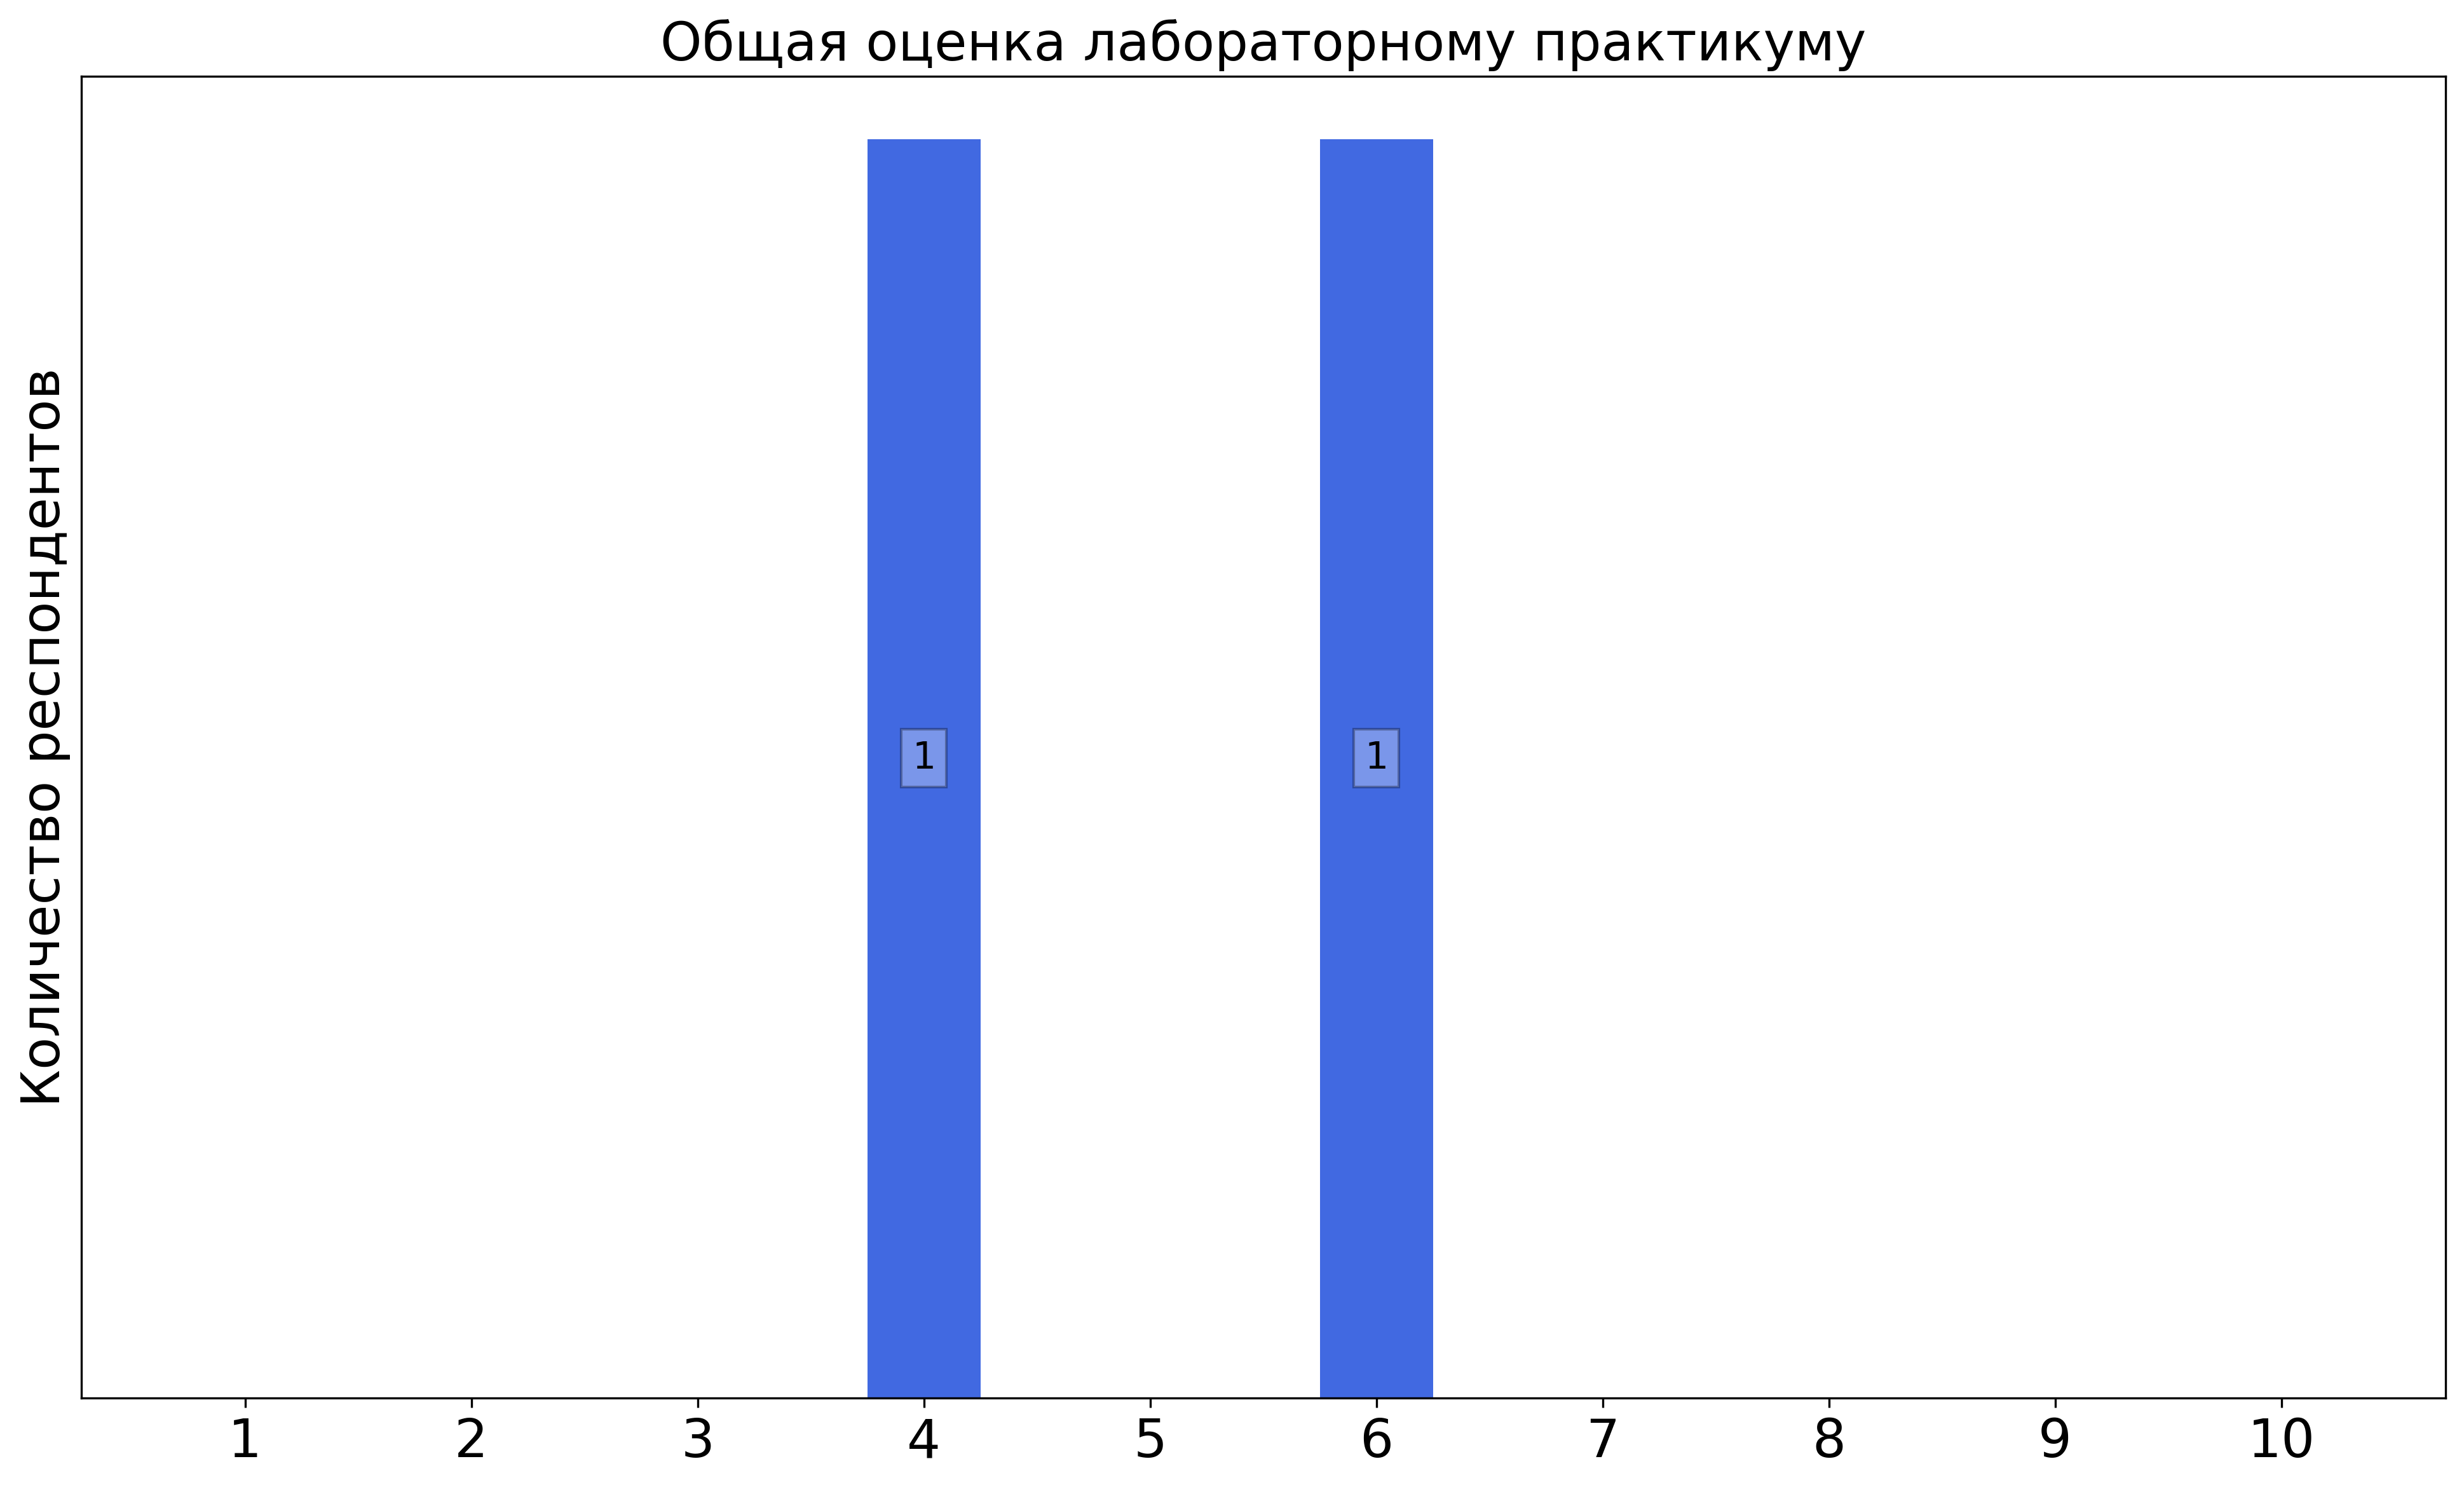
\includegraphics[width=\textwidth]{images/2 course/Радиотехнические цепи и сигналы/labniks-marks-Двойнишников Д.А. -3.png}
			\end{subfigure}	
			\caption{Оценки респондентов о качестве преподавания лабораторных работ}
		\end{figure}


    
    \subsubsection{Отзыв студентов о лабораторных работах. Преподаватель: Демин Д.А.}
		\begin{figure}[H]
			\centering
			\begin{subfigure}[b]{0.45\textwidth}
				\centering
				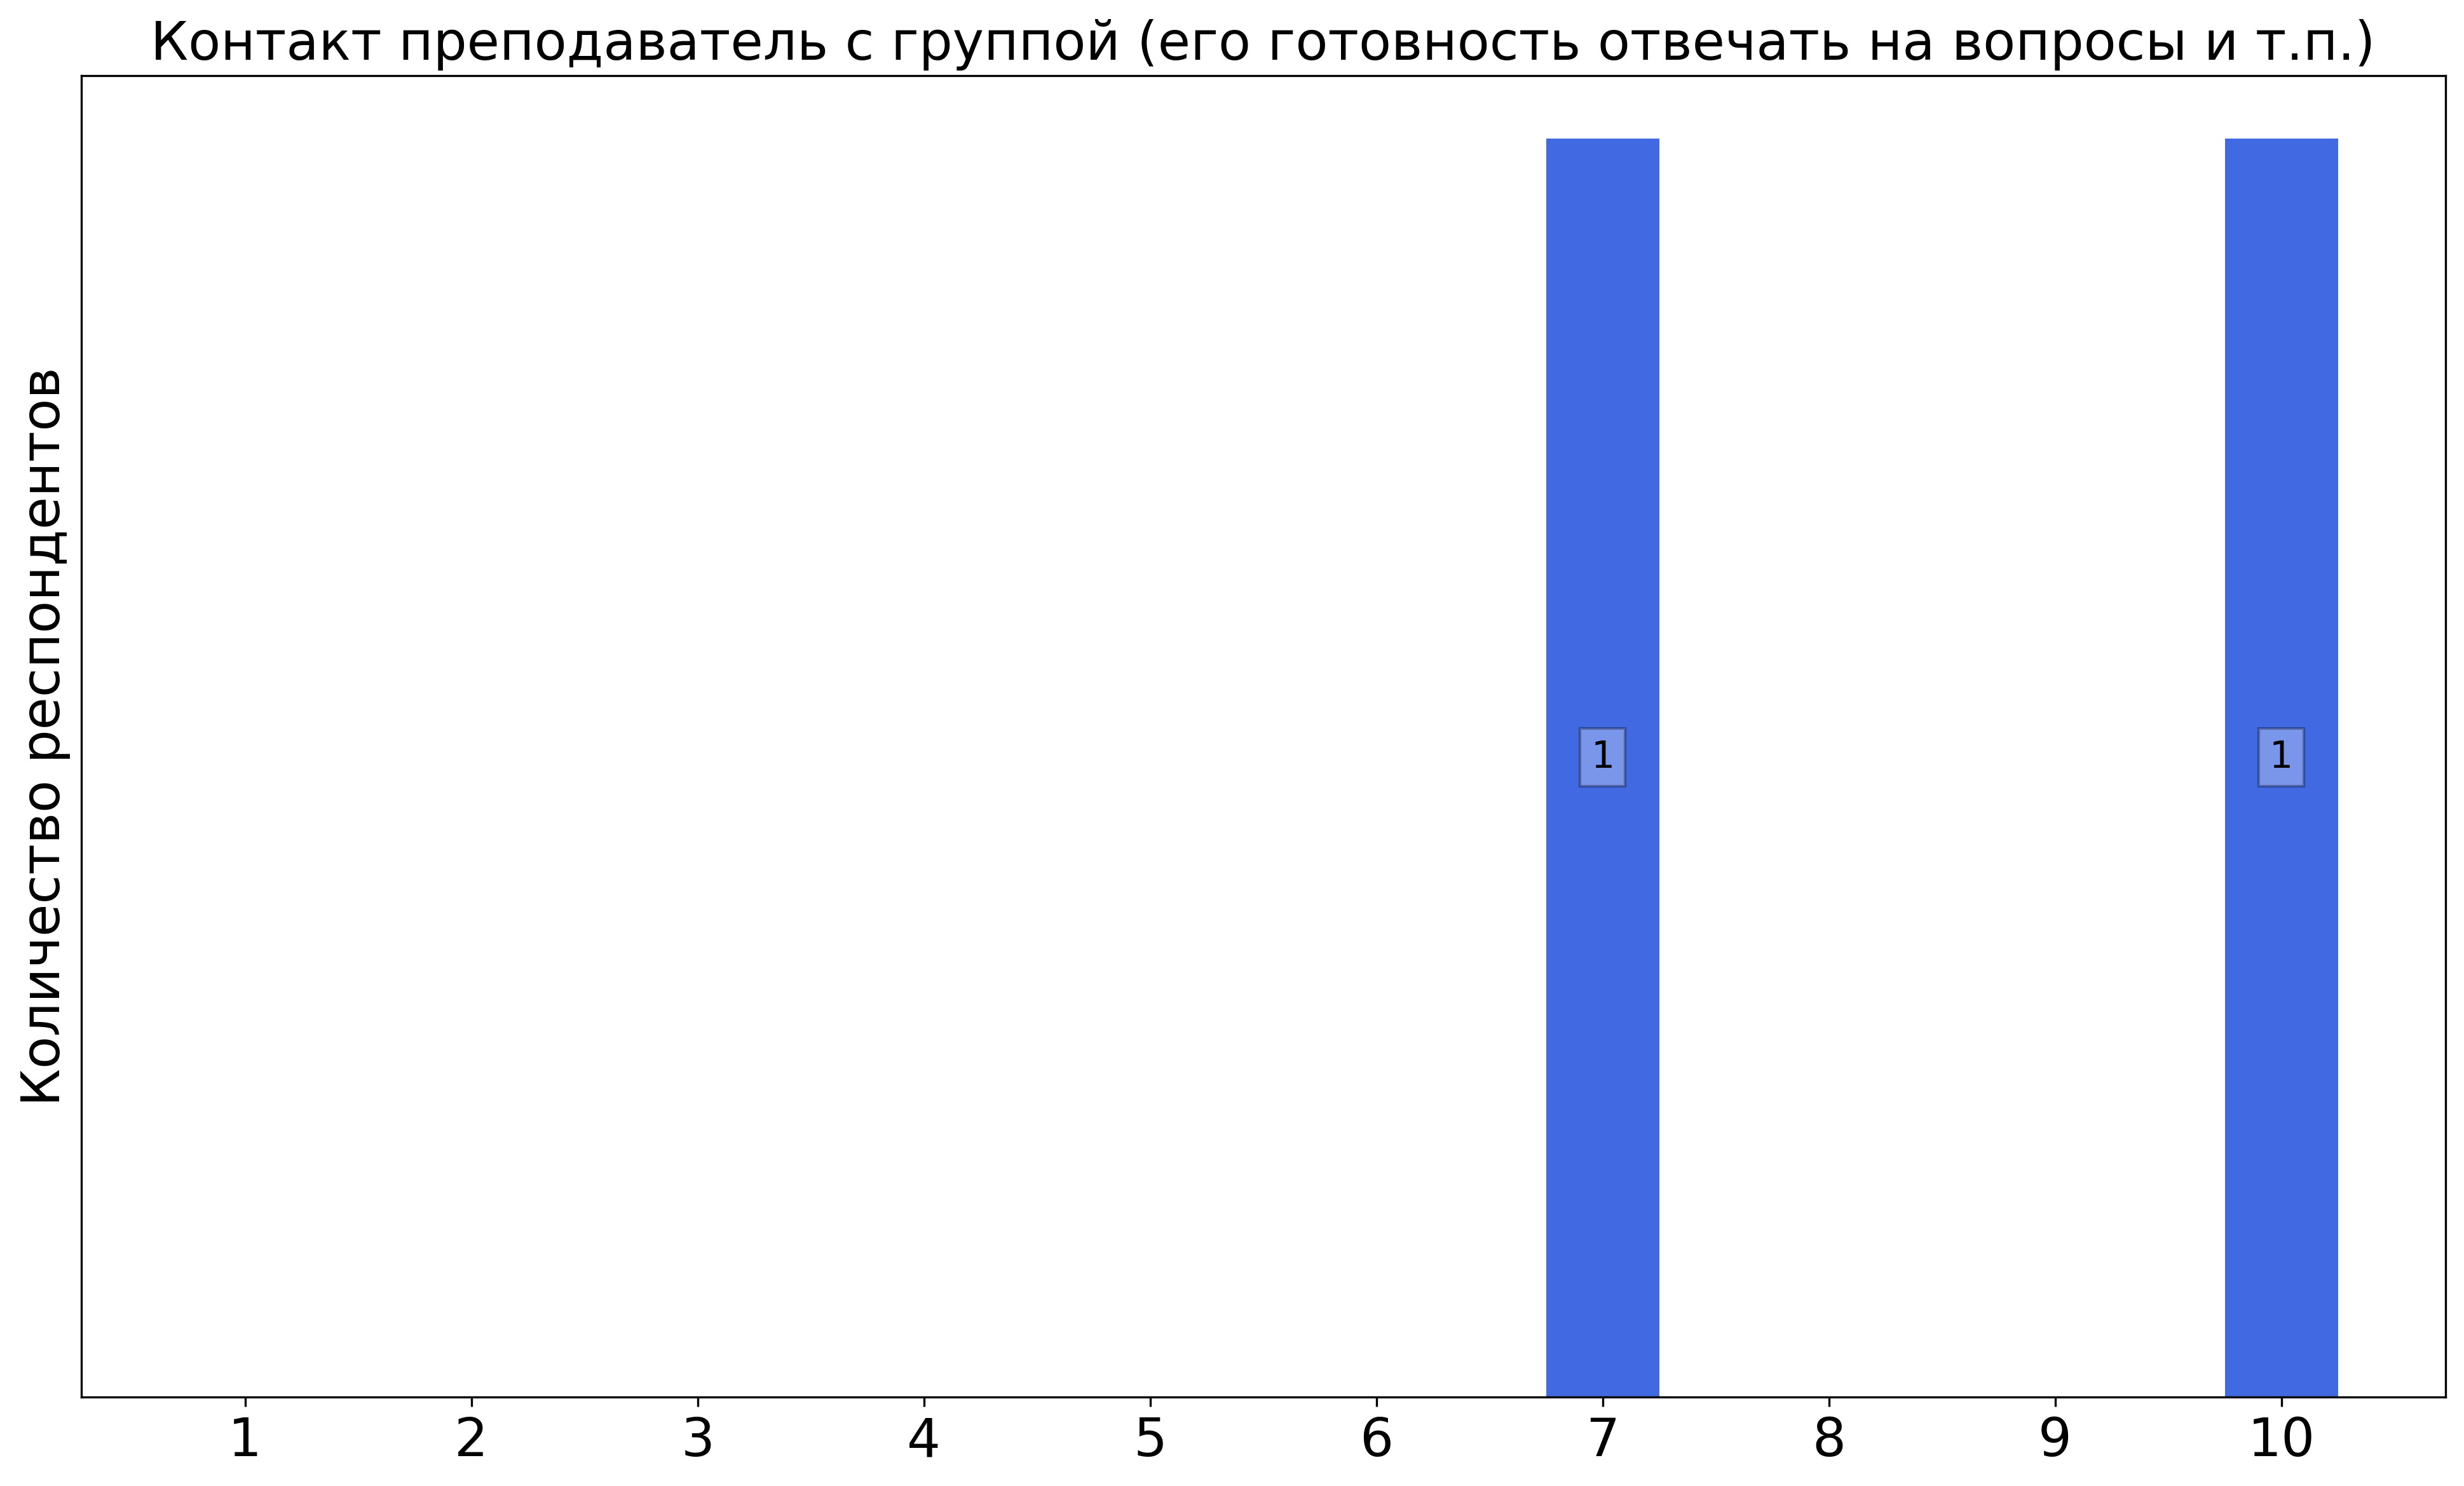
\includegraphics[width=\textwidth]{images/2 course/Радиотехнические цепи и сигналы/labniks-marks-Демин Д.А.-0.png}
			\end{subfigure}
			\begin{subfigure}[b]{0.45\textwidth}
				\centering
				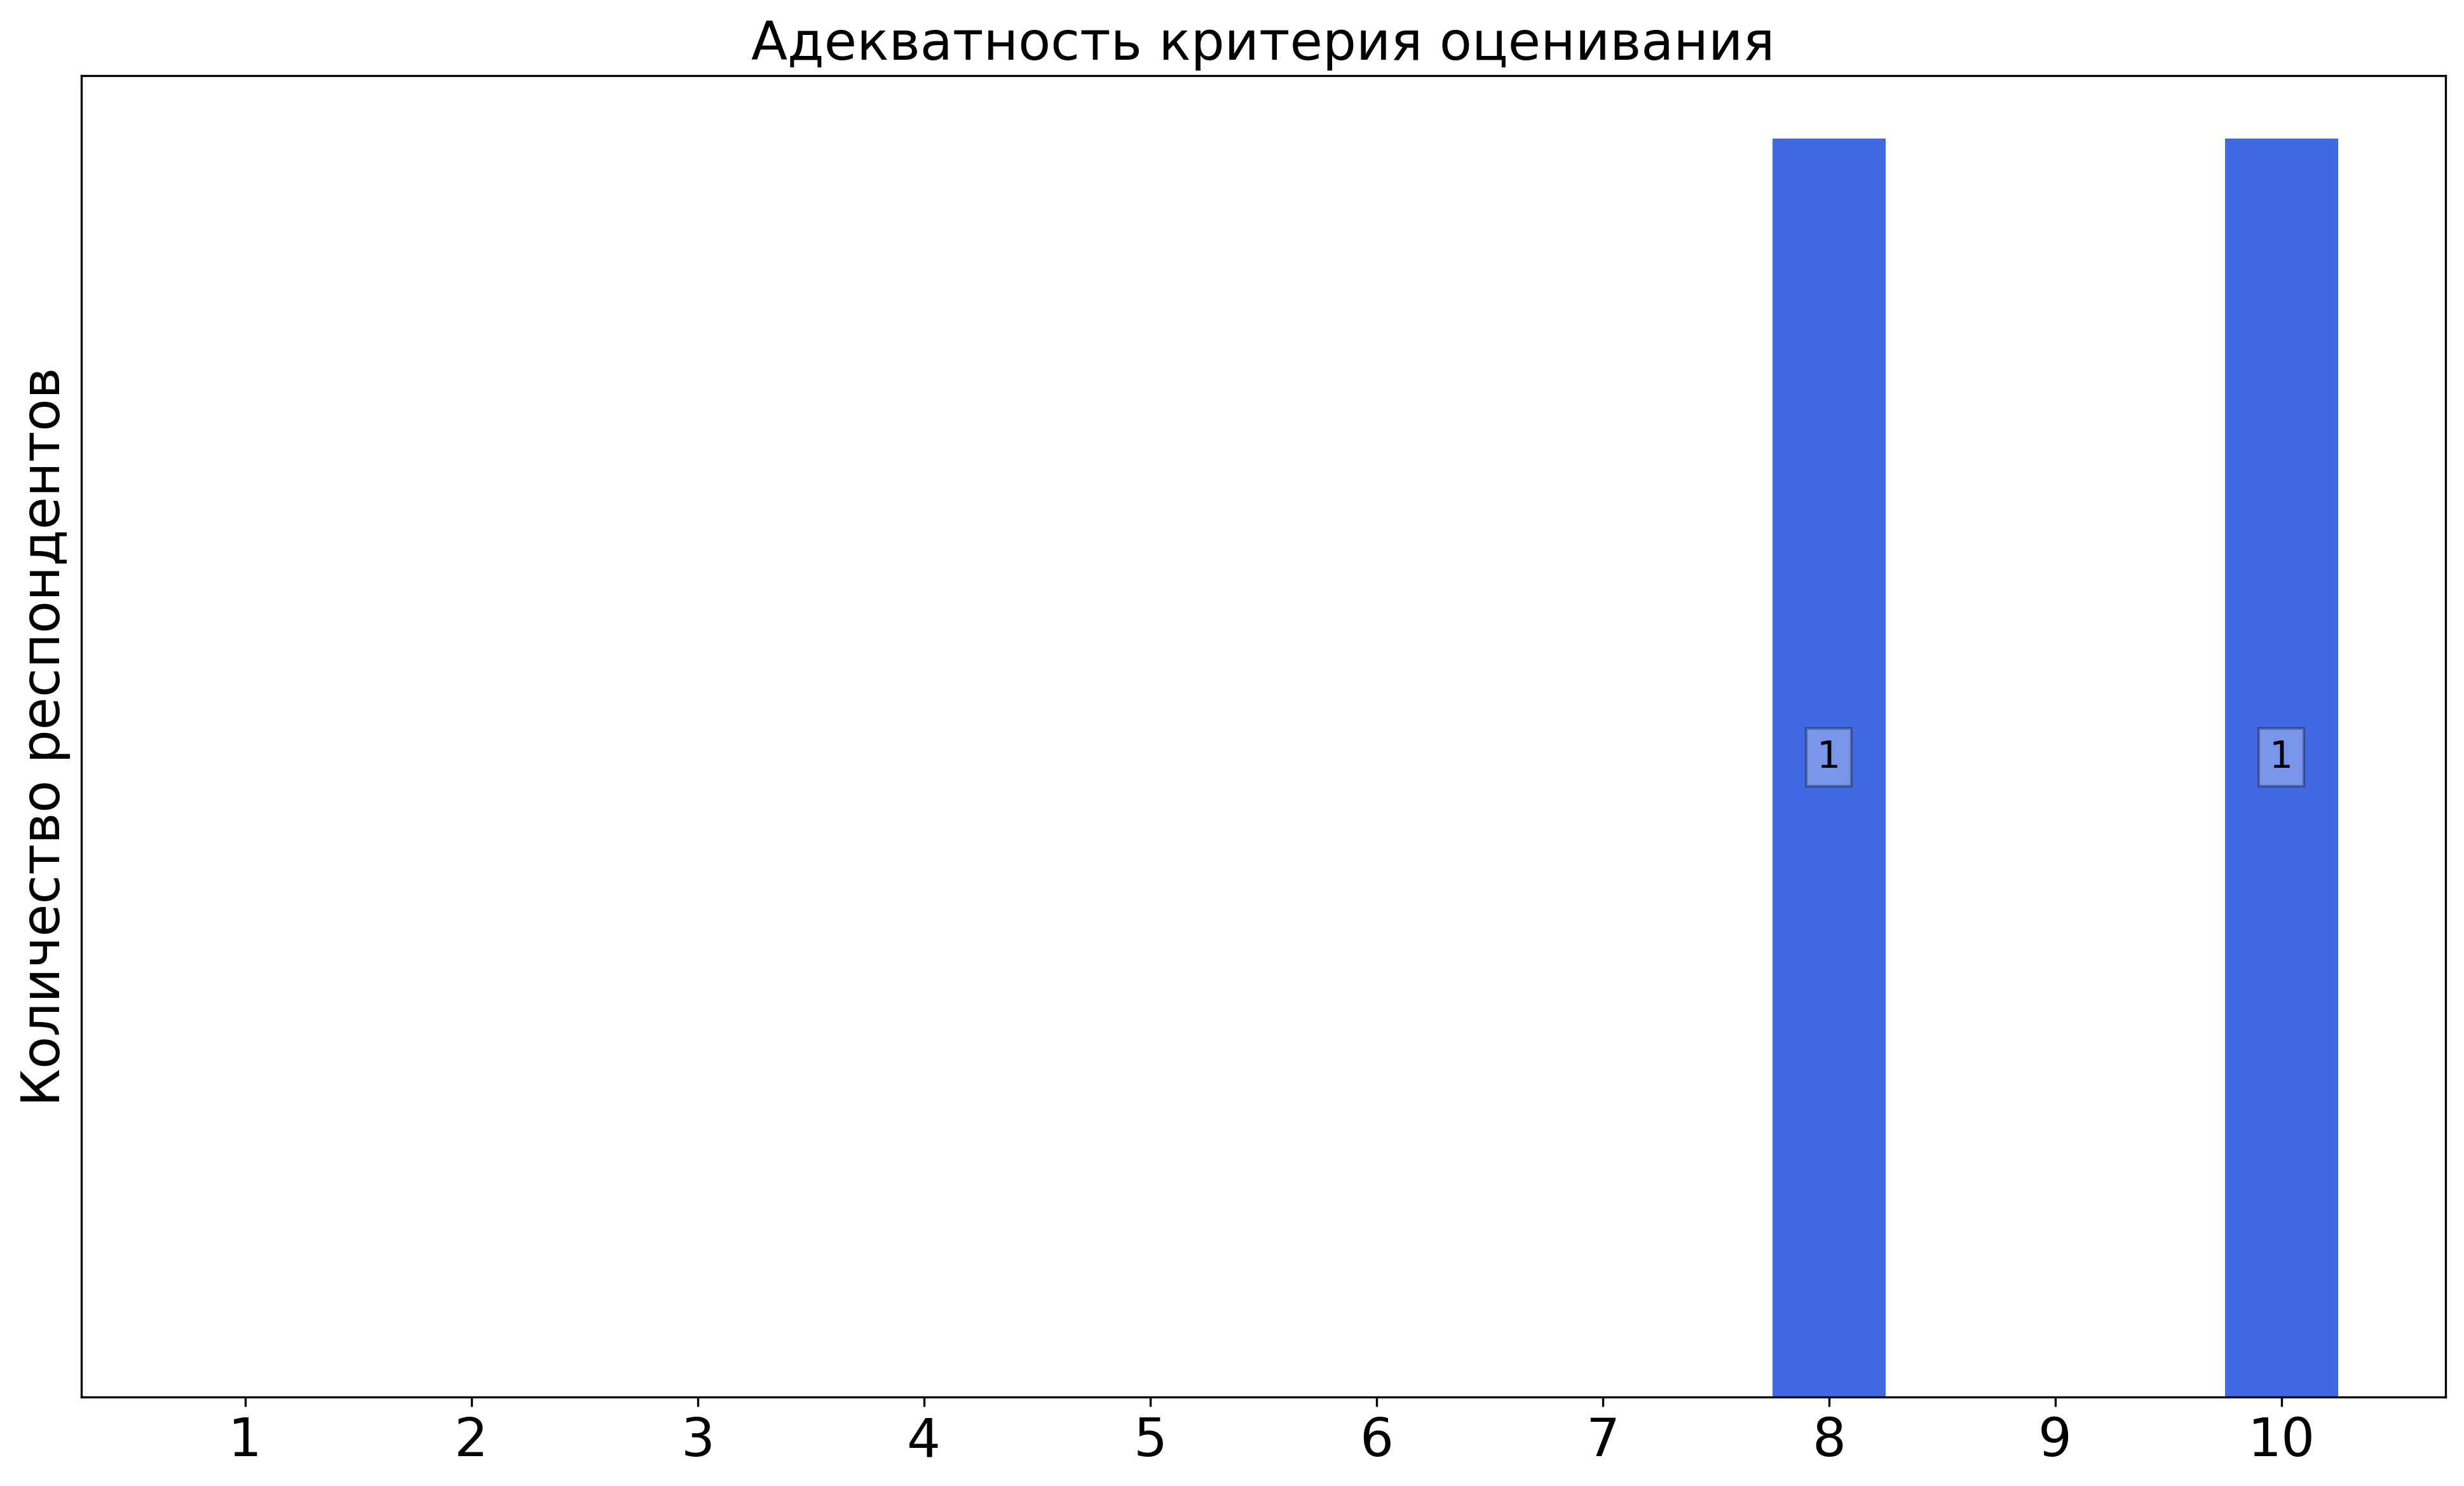
\includegraphics[width=\textwidth]{images/2 course/Радиотехнические цепи и сигналы/labniks-marks-Демин Д.А.-1.png}
			\end{subfigure}
			\begin{subfigure}[b]{0.45\textwidth}
				\centering
				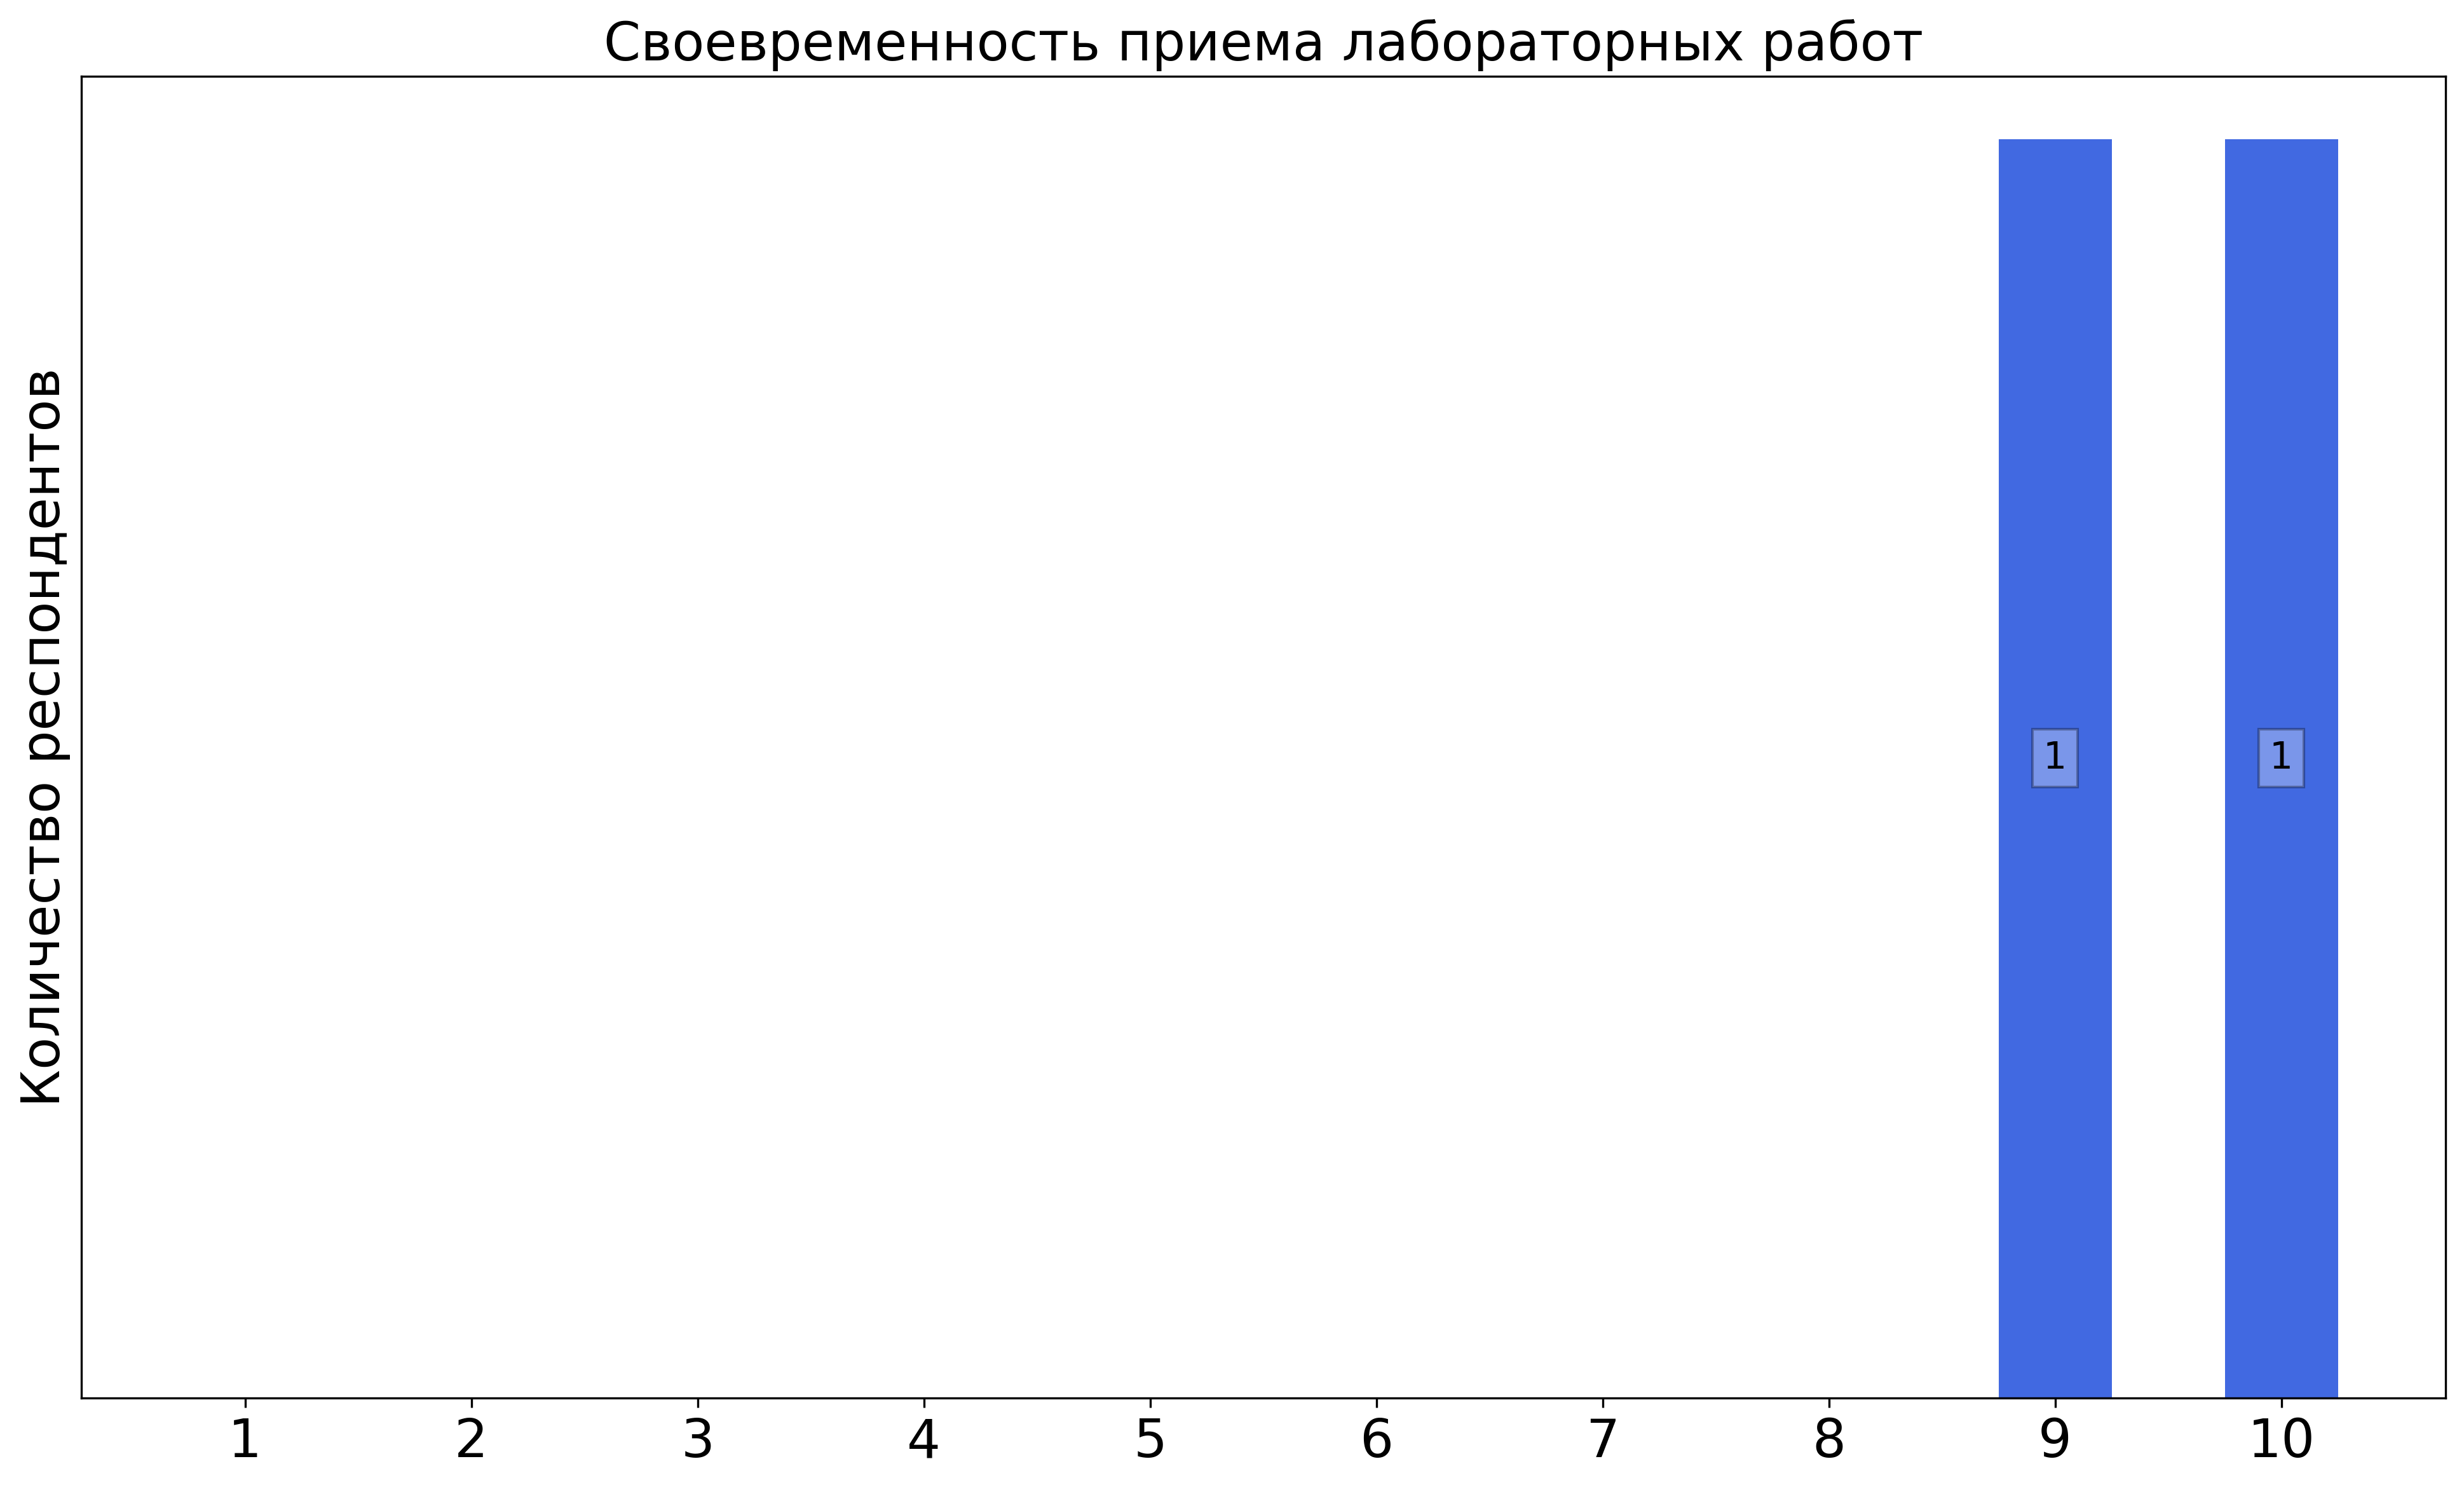
\includegraphics[width=\textwidth]{images/2 course/Радиотехнические цепи и сигналы/labniks-marks-Демин Д.А.-2.png}
			\end{subfigure}
			\begin{subfigure}[b]{0.45\textwidth}
				\centering
				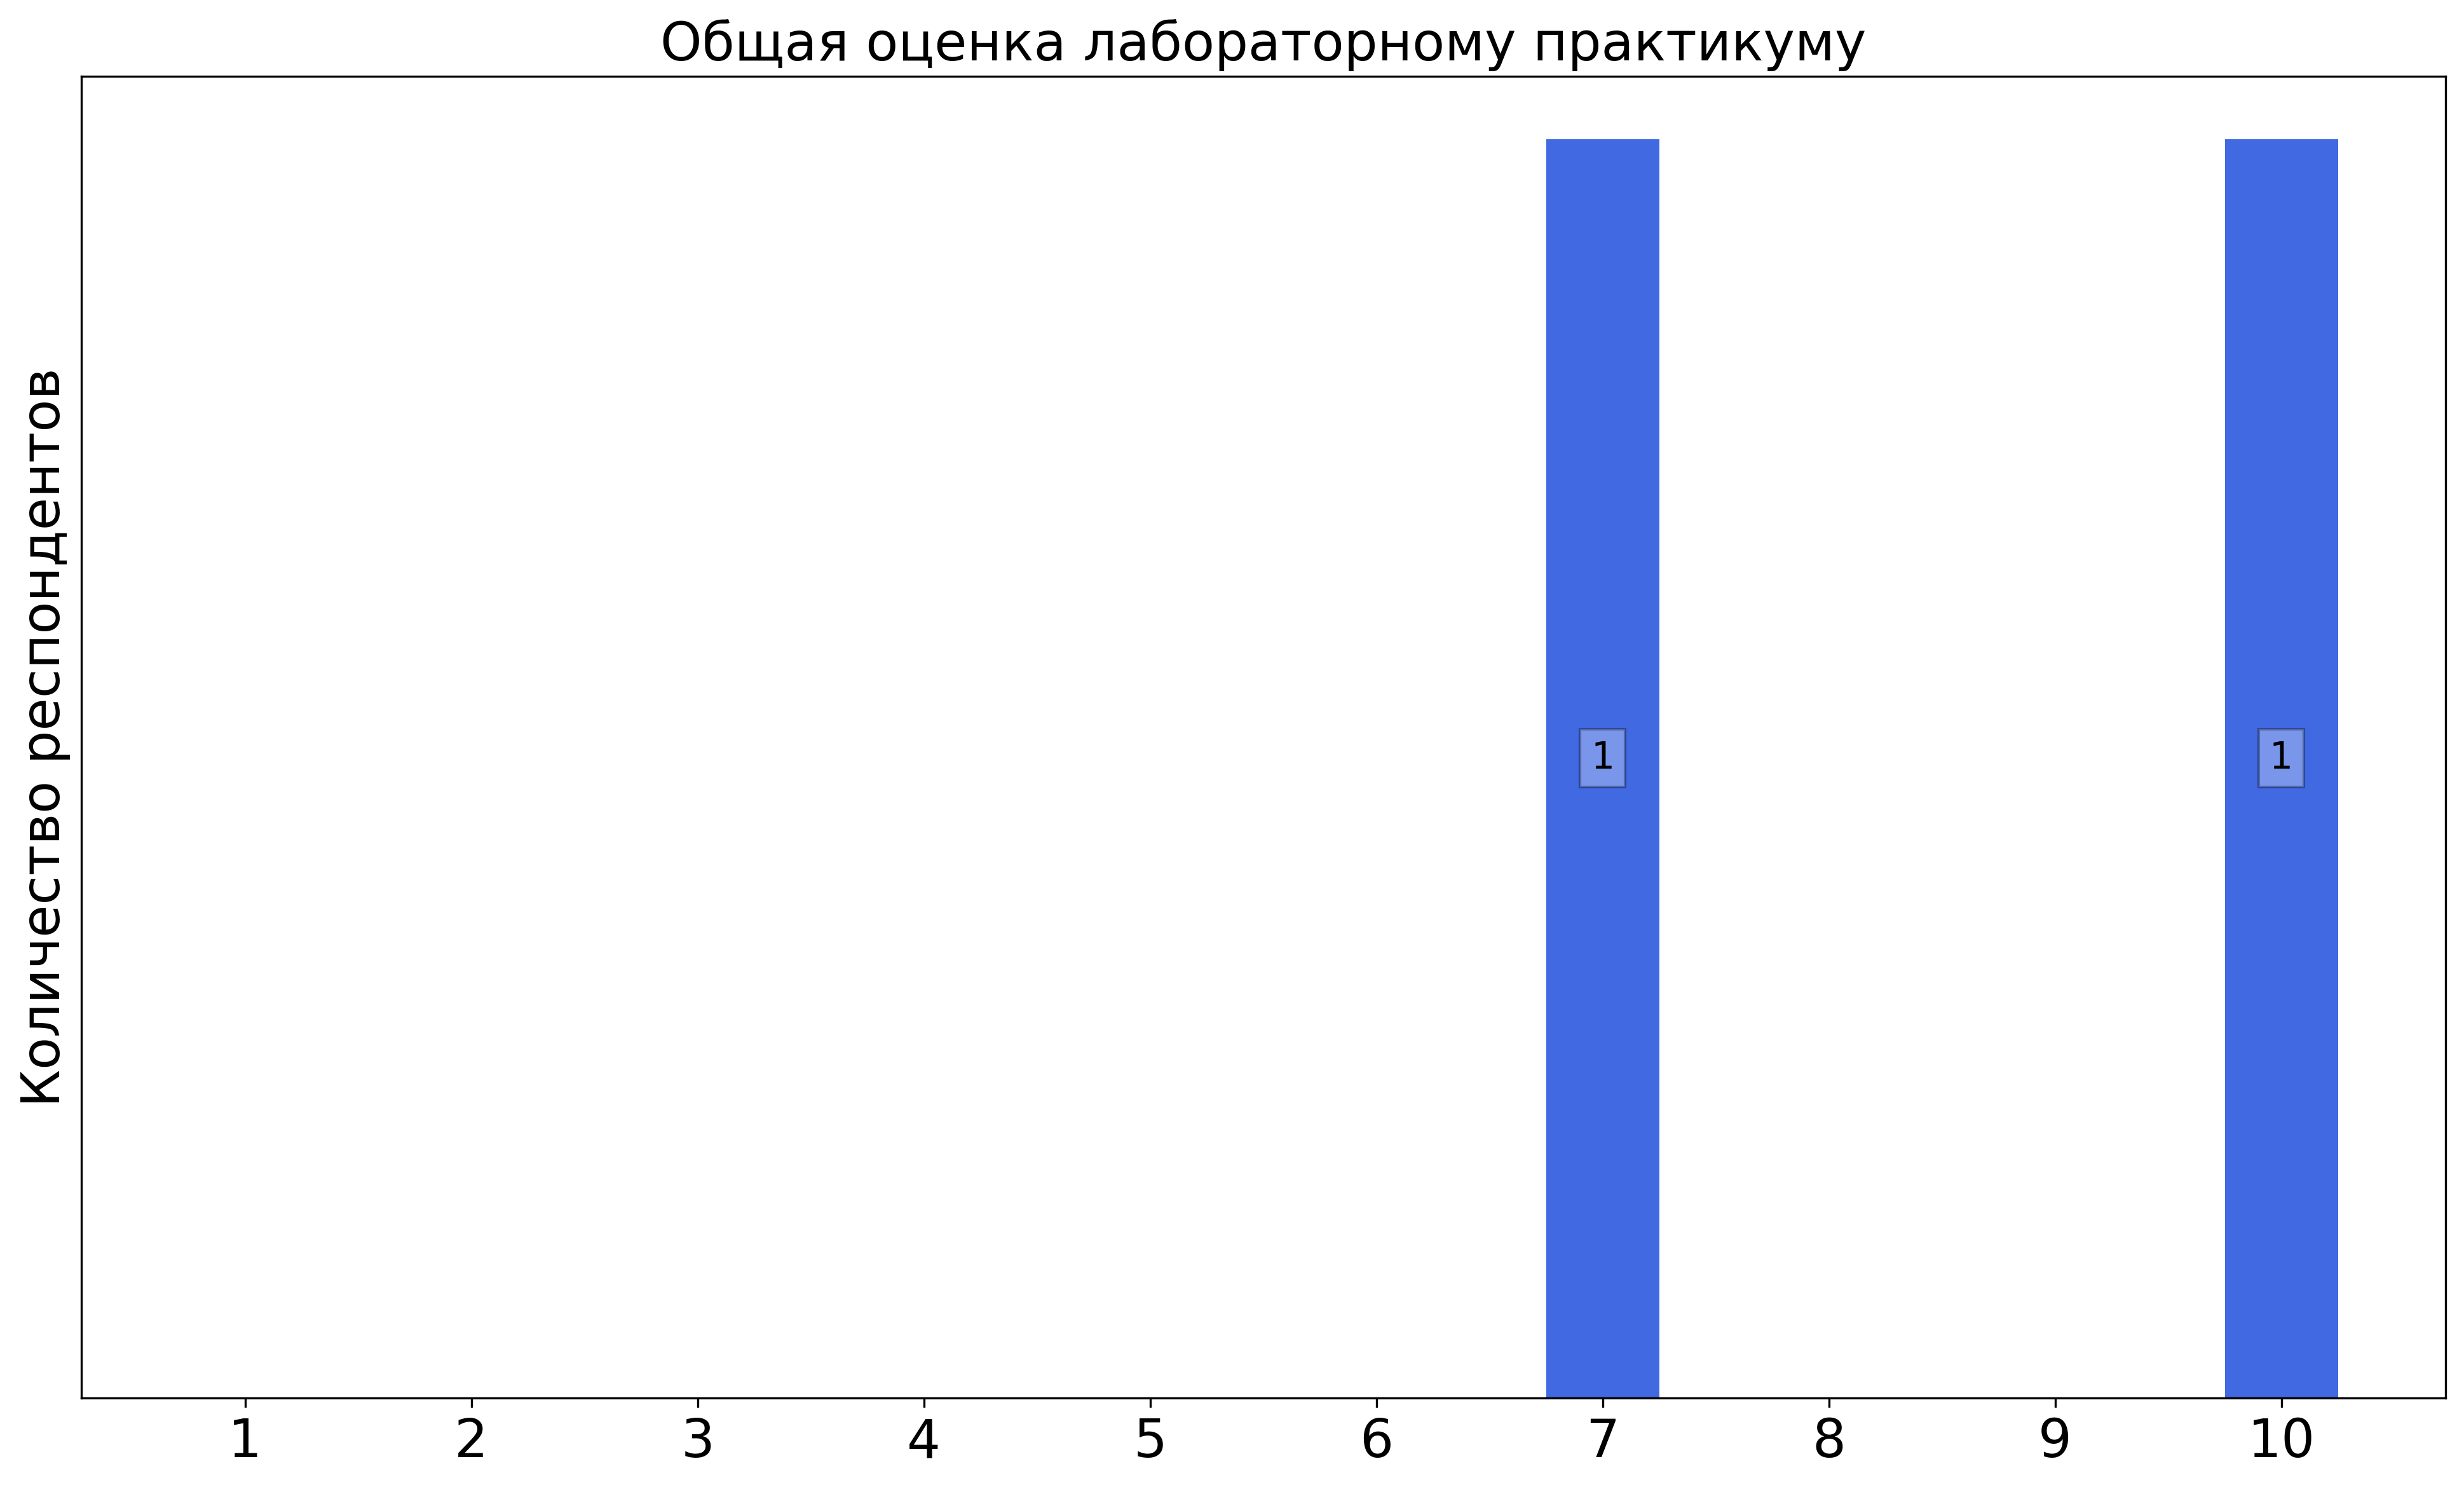
\includegraphics[width=\textwidth]{images/2 course/Радиотехнические цепи и сигналы/labniks-marks-Демин Д.А.-3.png}
			\end{subfigure}	
			\caption{Оценки респондентов о качестве преподавания лабораторных работ}
		\end{figure}


    
    \subsubsection{Отзыв студентов о лабораторных работах. Преподаватель: Дудкин П.В.}
		\begin{figure}[H]
			\centering
			\begin{subfigure}[b]{0.45\textwidth}
				\centering
				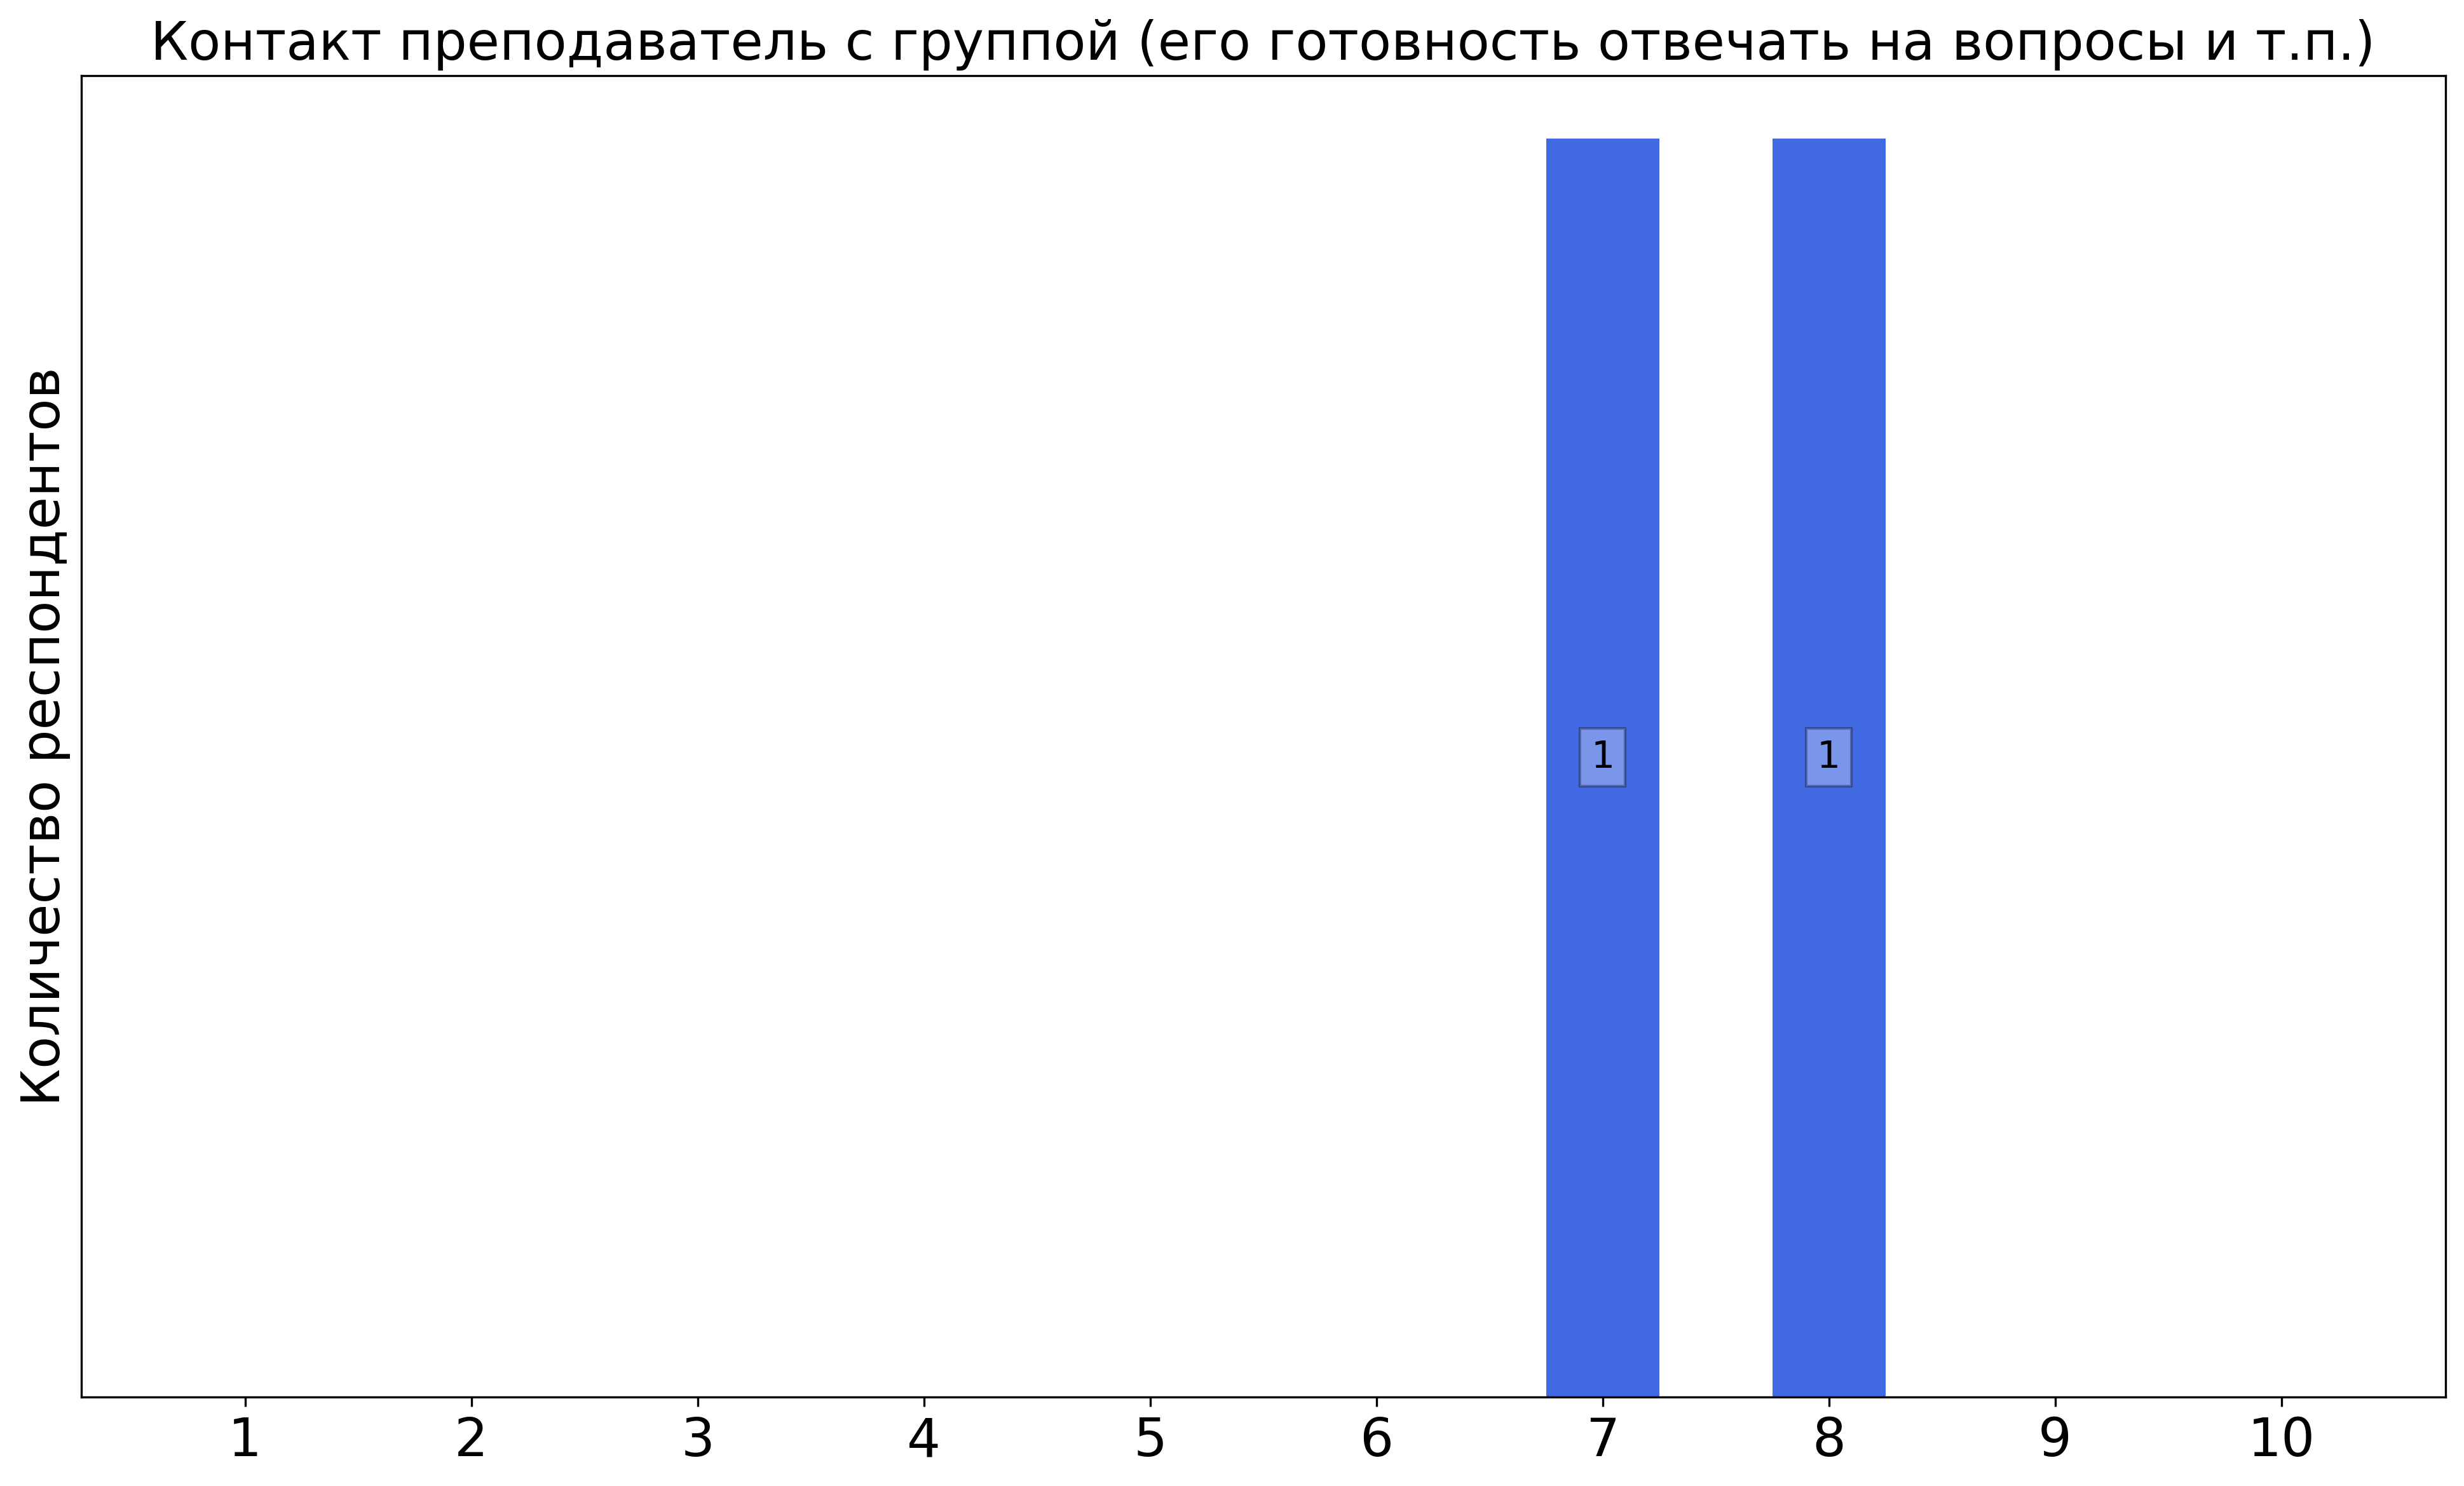
\includegraphics[width=\textwidth]{images/2 course/Радиотехнические цепи и сигналы/labniks-marks-Дудкин П.В.-0.png}
			\end{subfigure}
			\begin{subfigure}[b]{0.45\textwidth}
				\centering
				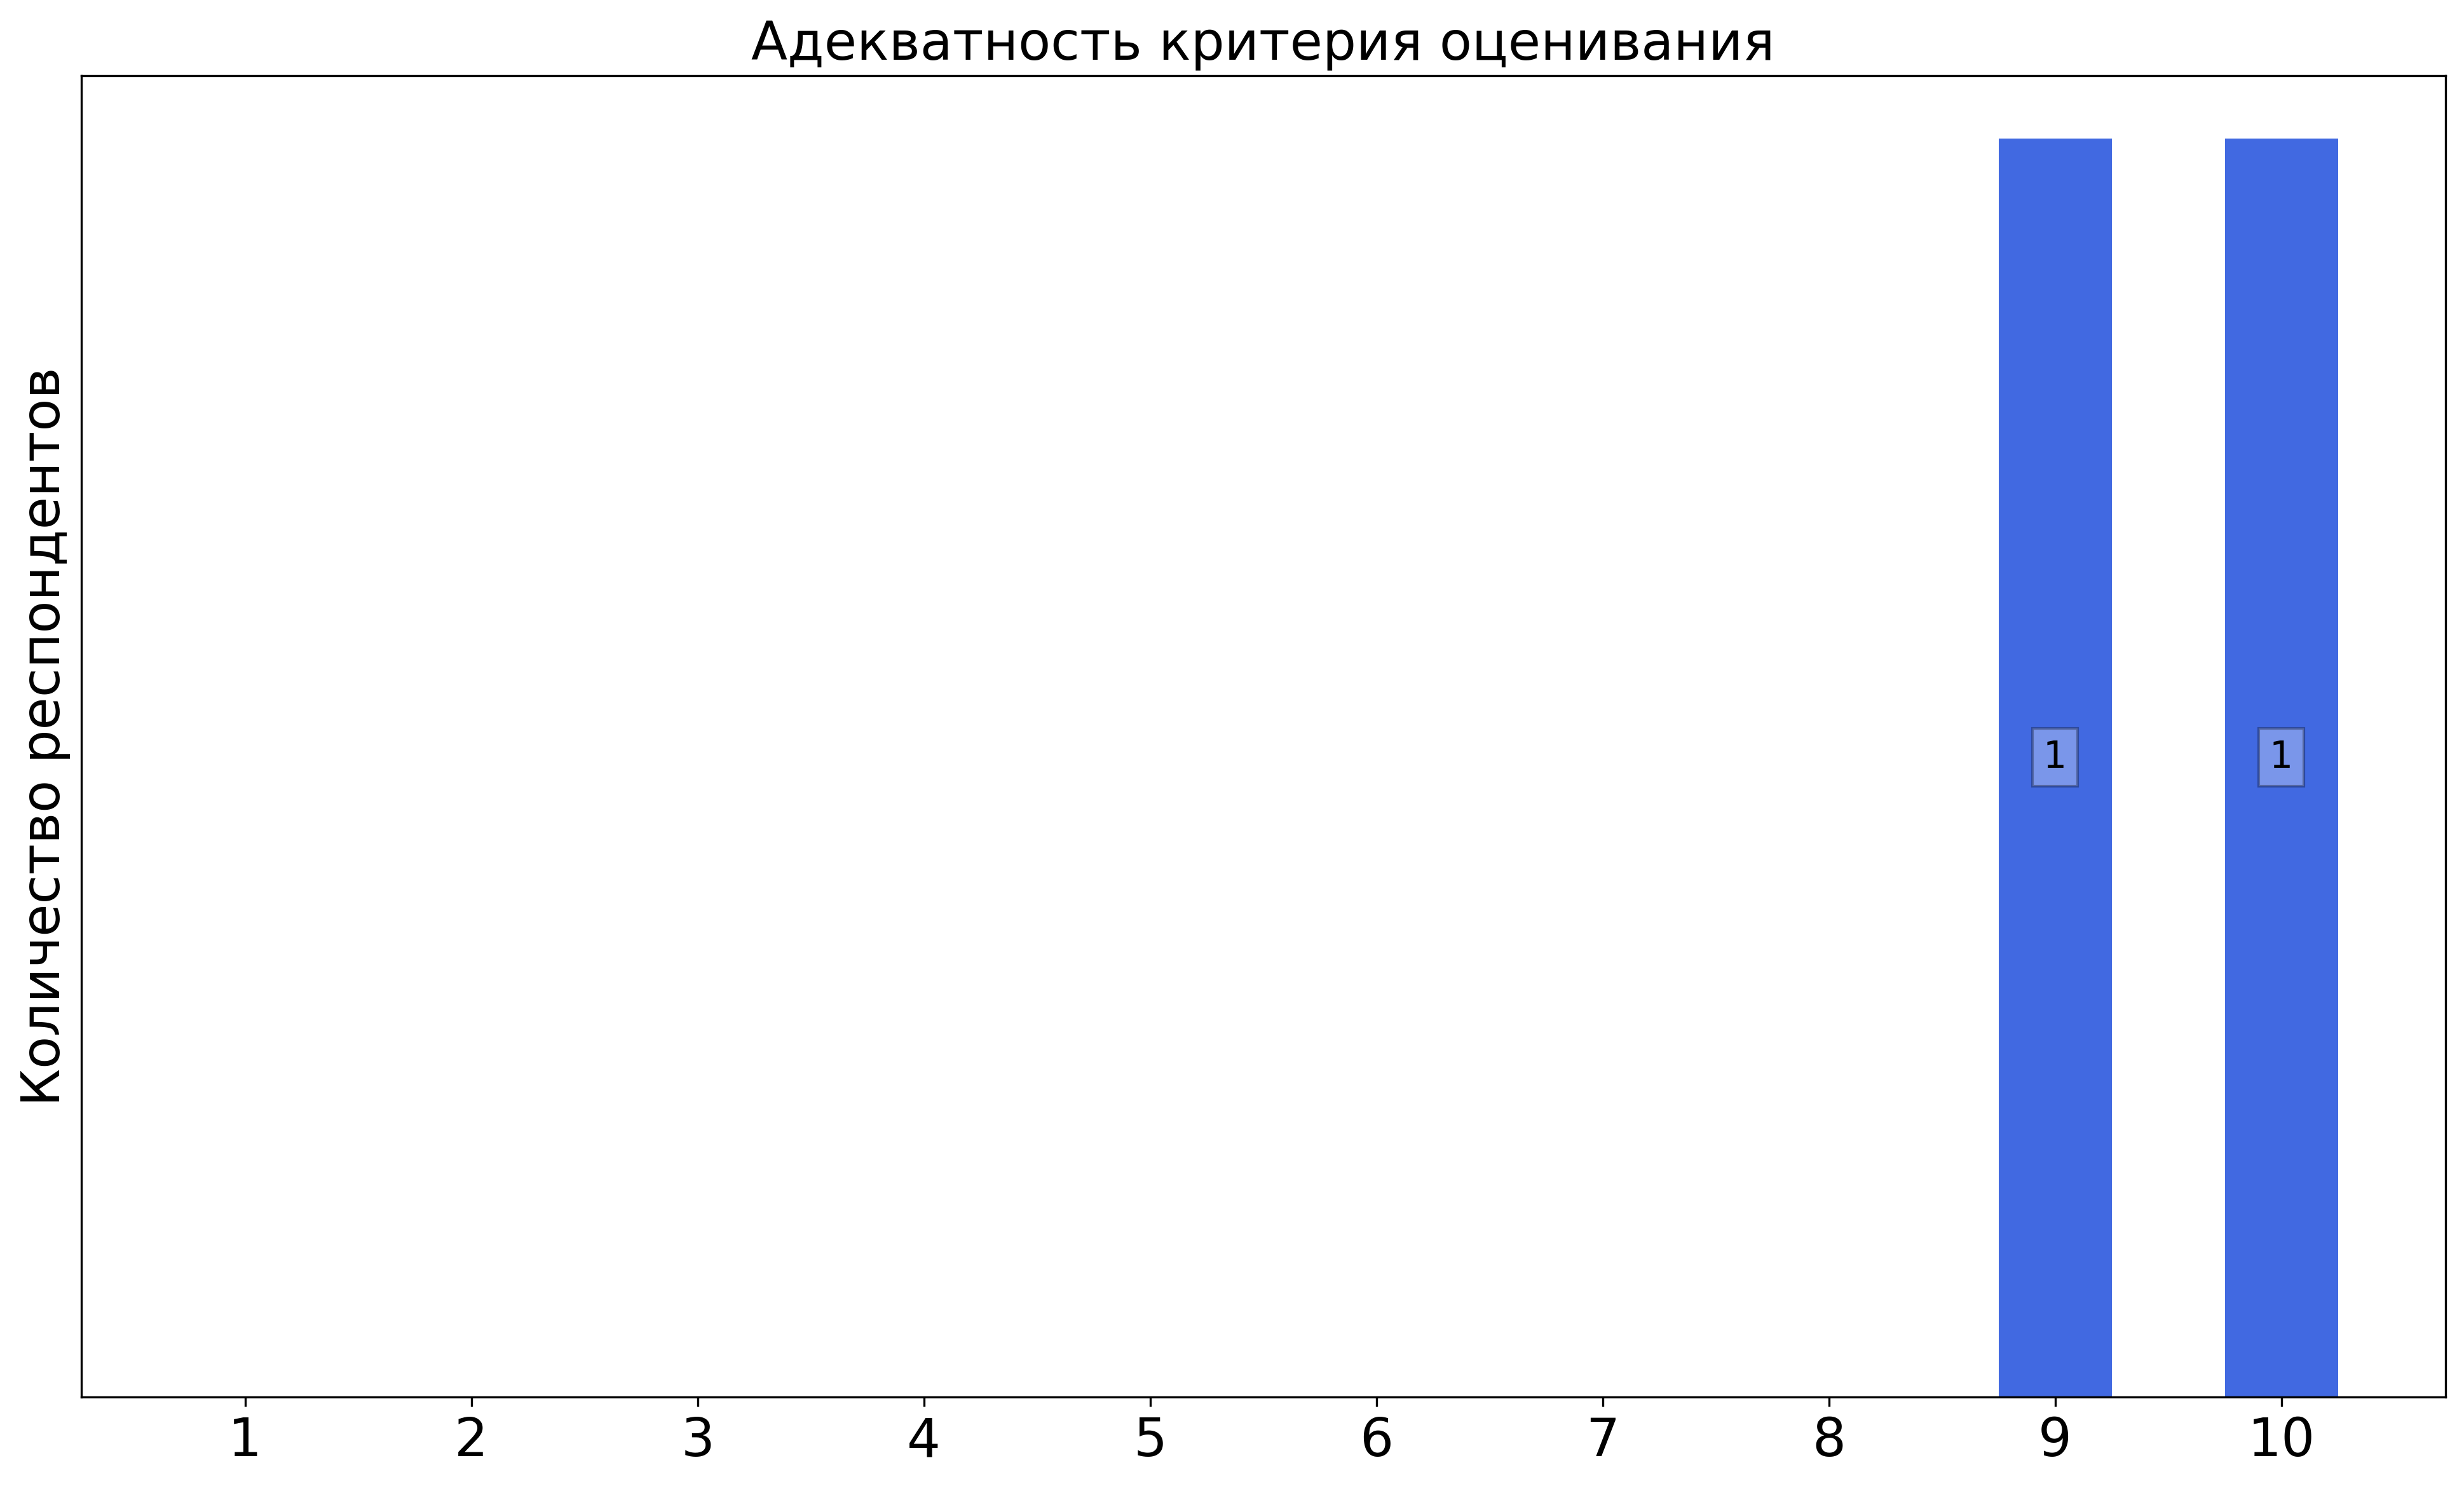
\includegraphics[width=\textwidth]{images/2 course/Радиотехнические цепи и сигналы/labniks-marks-Дудкин П.В.-1.png}
			\end{subfigure}
			\begin{subfigure}[b]{0.45\textwidth}
				\centering
				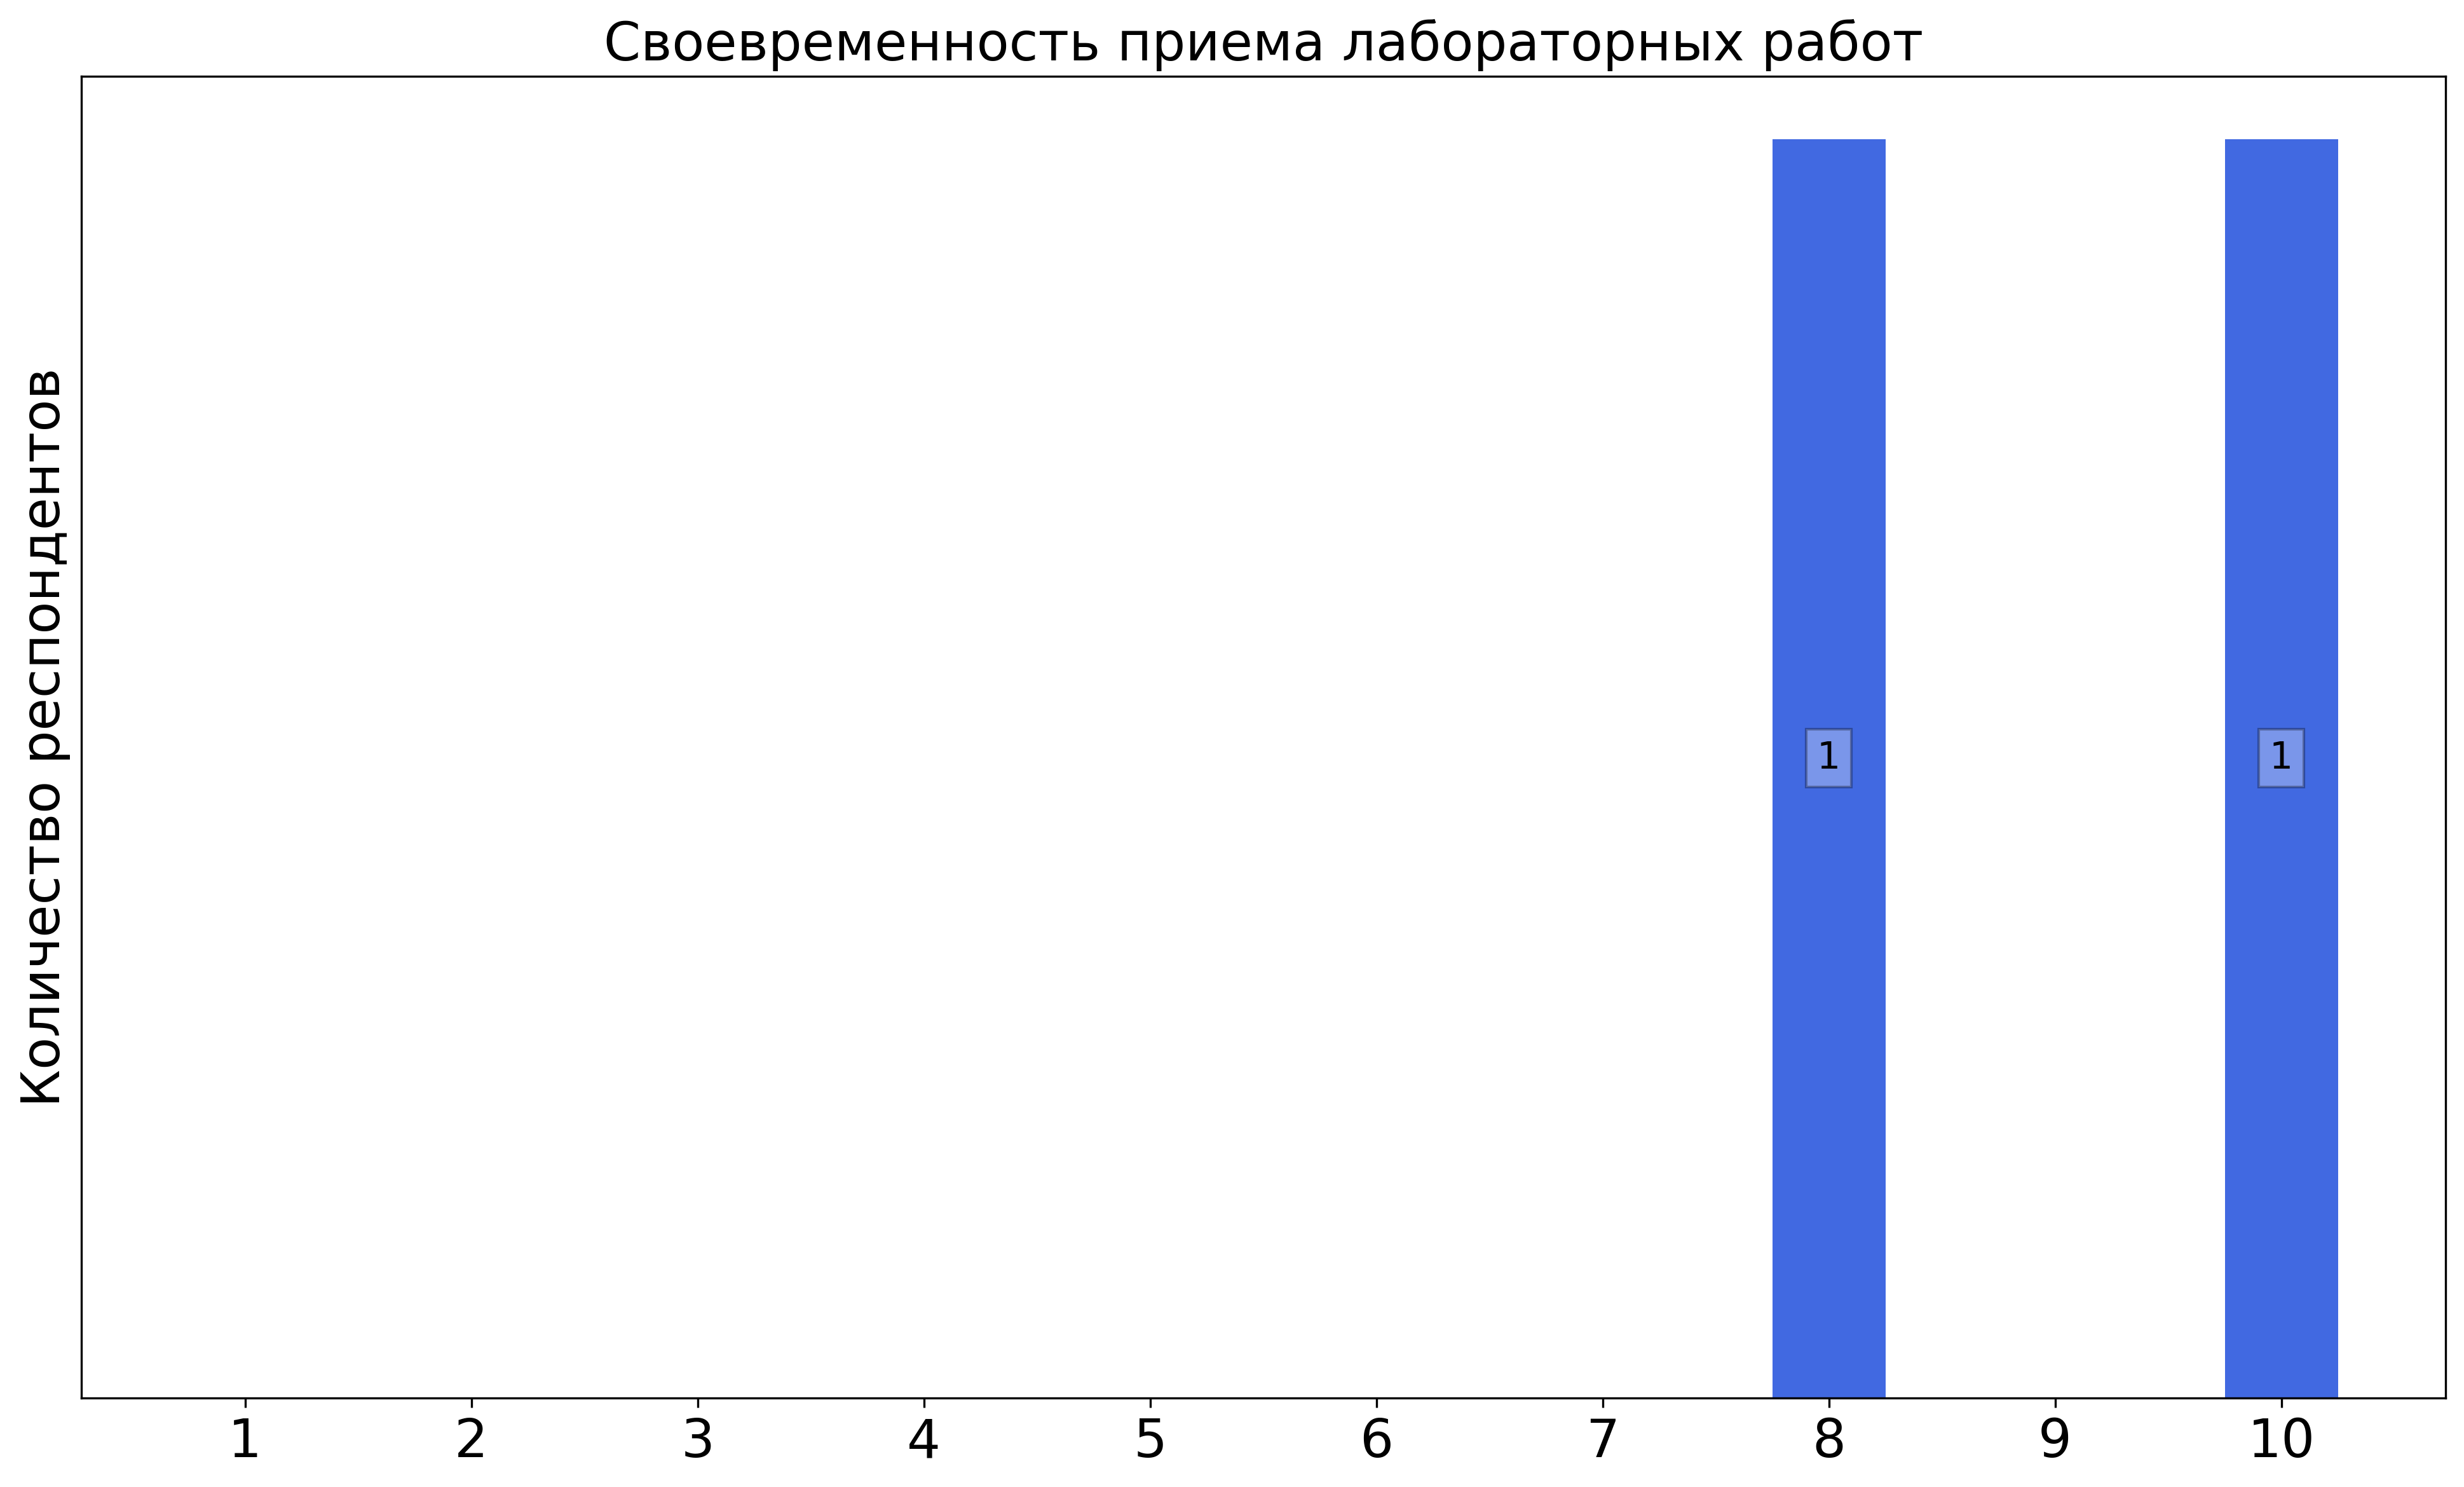
\includegraphics[width=\textwidth]{images/2 course/Радиотехнические цепи и сигналы/labniks-marks-Дудкин П.В.-2.png}
			\end{subfigure}
			\begin{subfigure}[b]{0.45\textwidth}
				\centering
				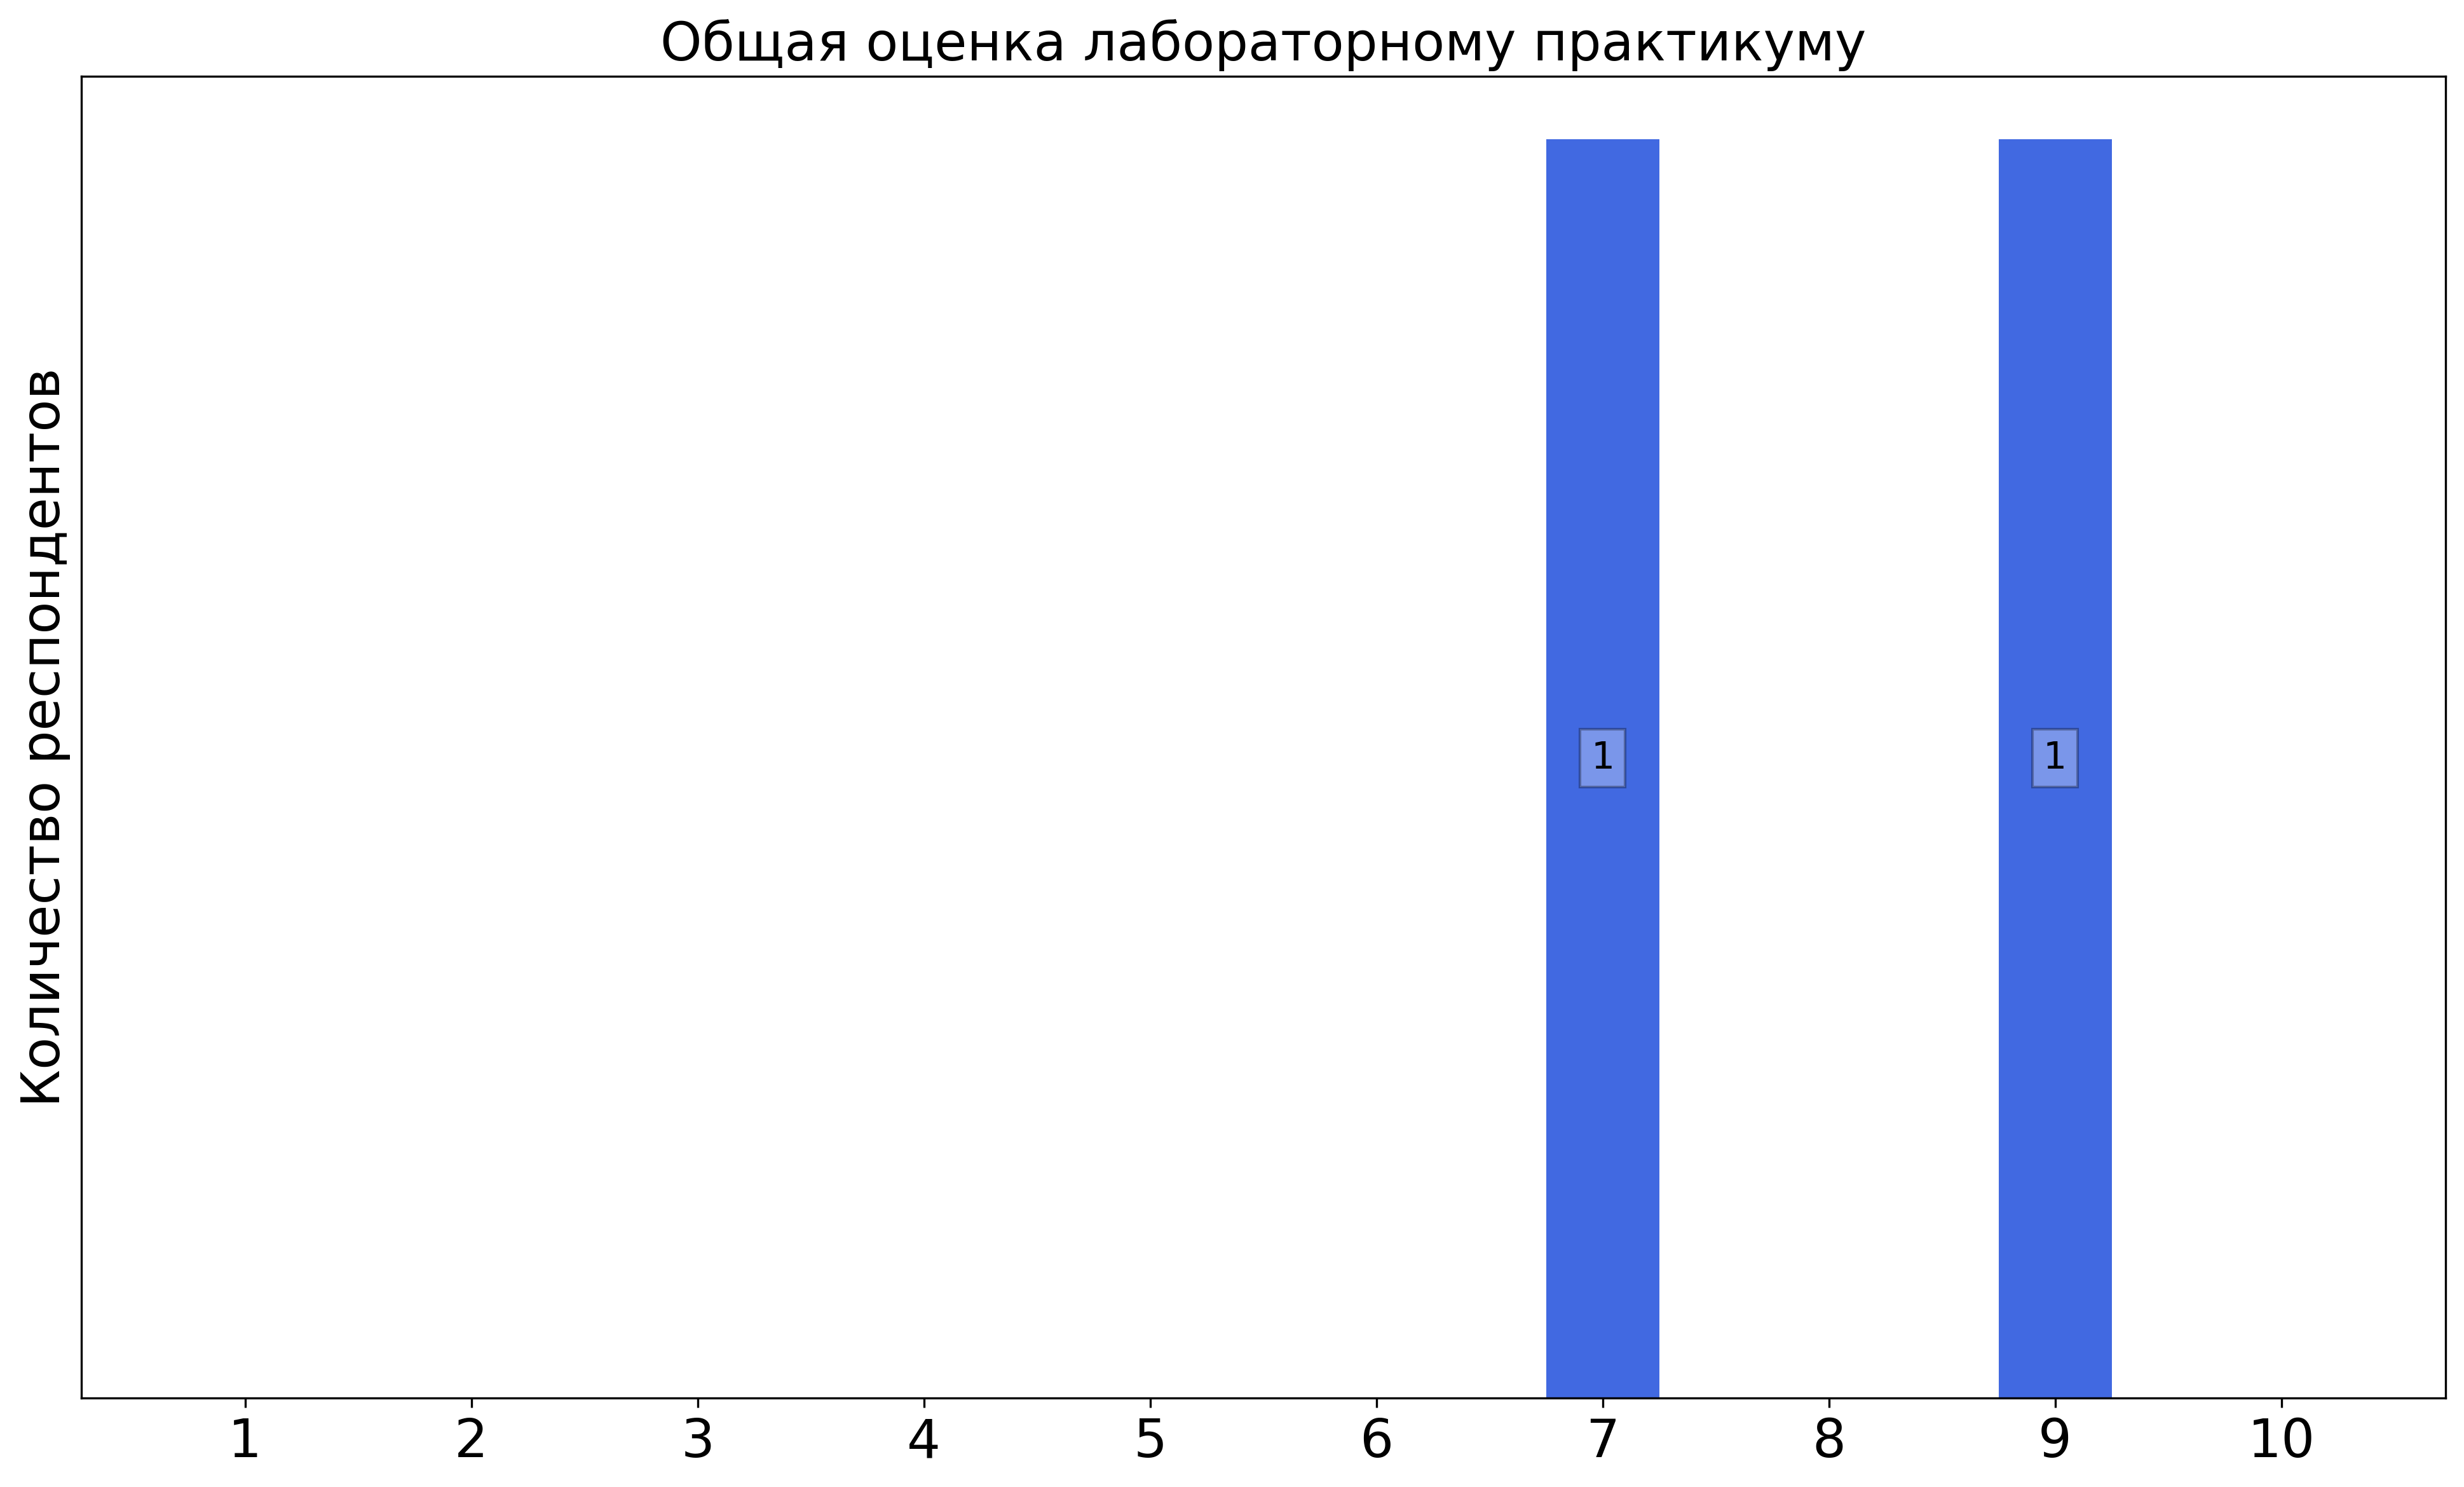
\includegraphics[width=\textwidth]{images/2 course/Радиотехнические цепи и сигналы/labniks-marks-Дудкин П.В.-3.png}
			\end{subfigure}	
			\caption{Оценки респондентов о качестве преподавания лабораторных работ}
		\end{figure}


        
    \subsubsection{Отзыв студентов о лабораторных работах. Преподаватель: Неешпапа А.В.}
        \begin{figure}[H]
            \centering
            \begin{subfigure}[b]{0.45\textwidth}
                \centering
                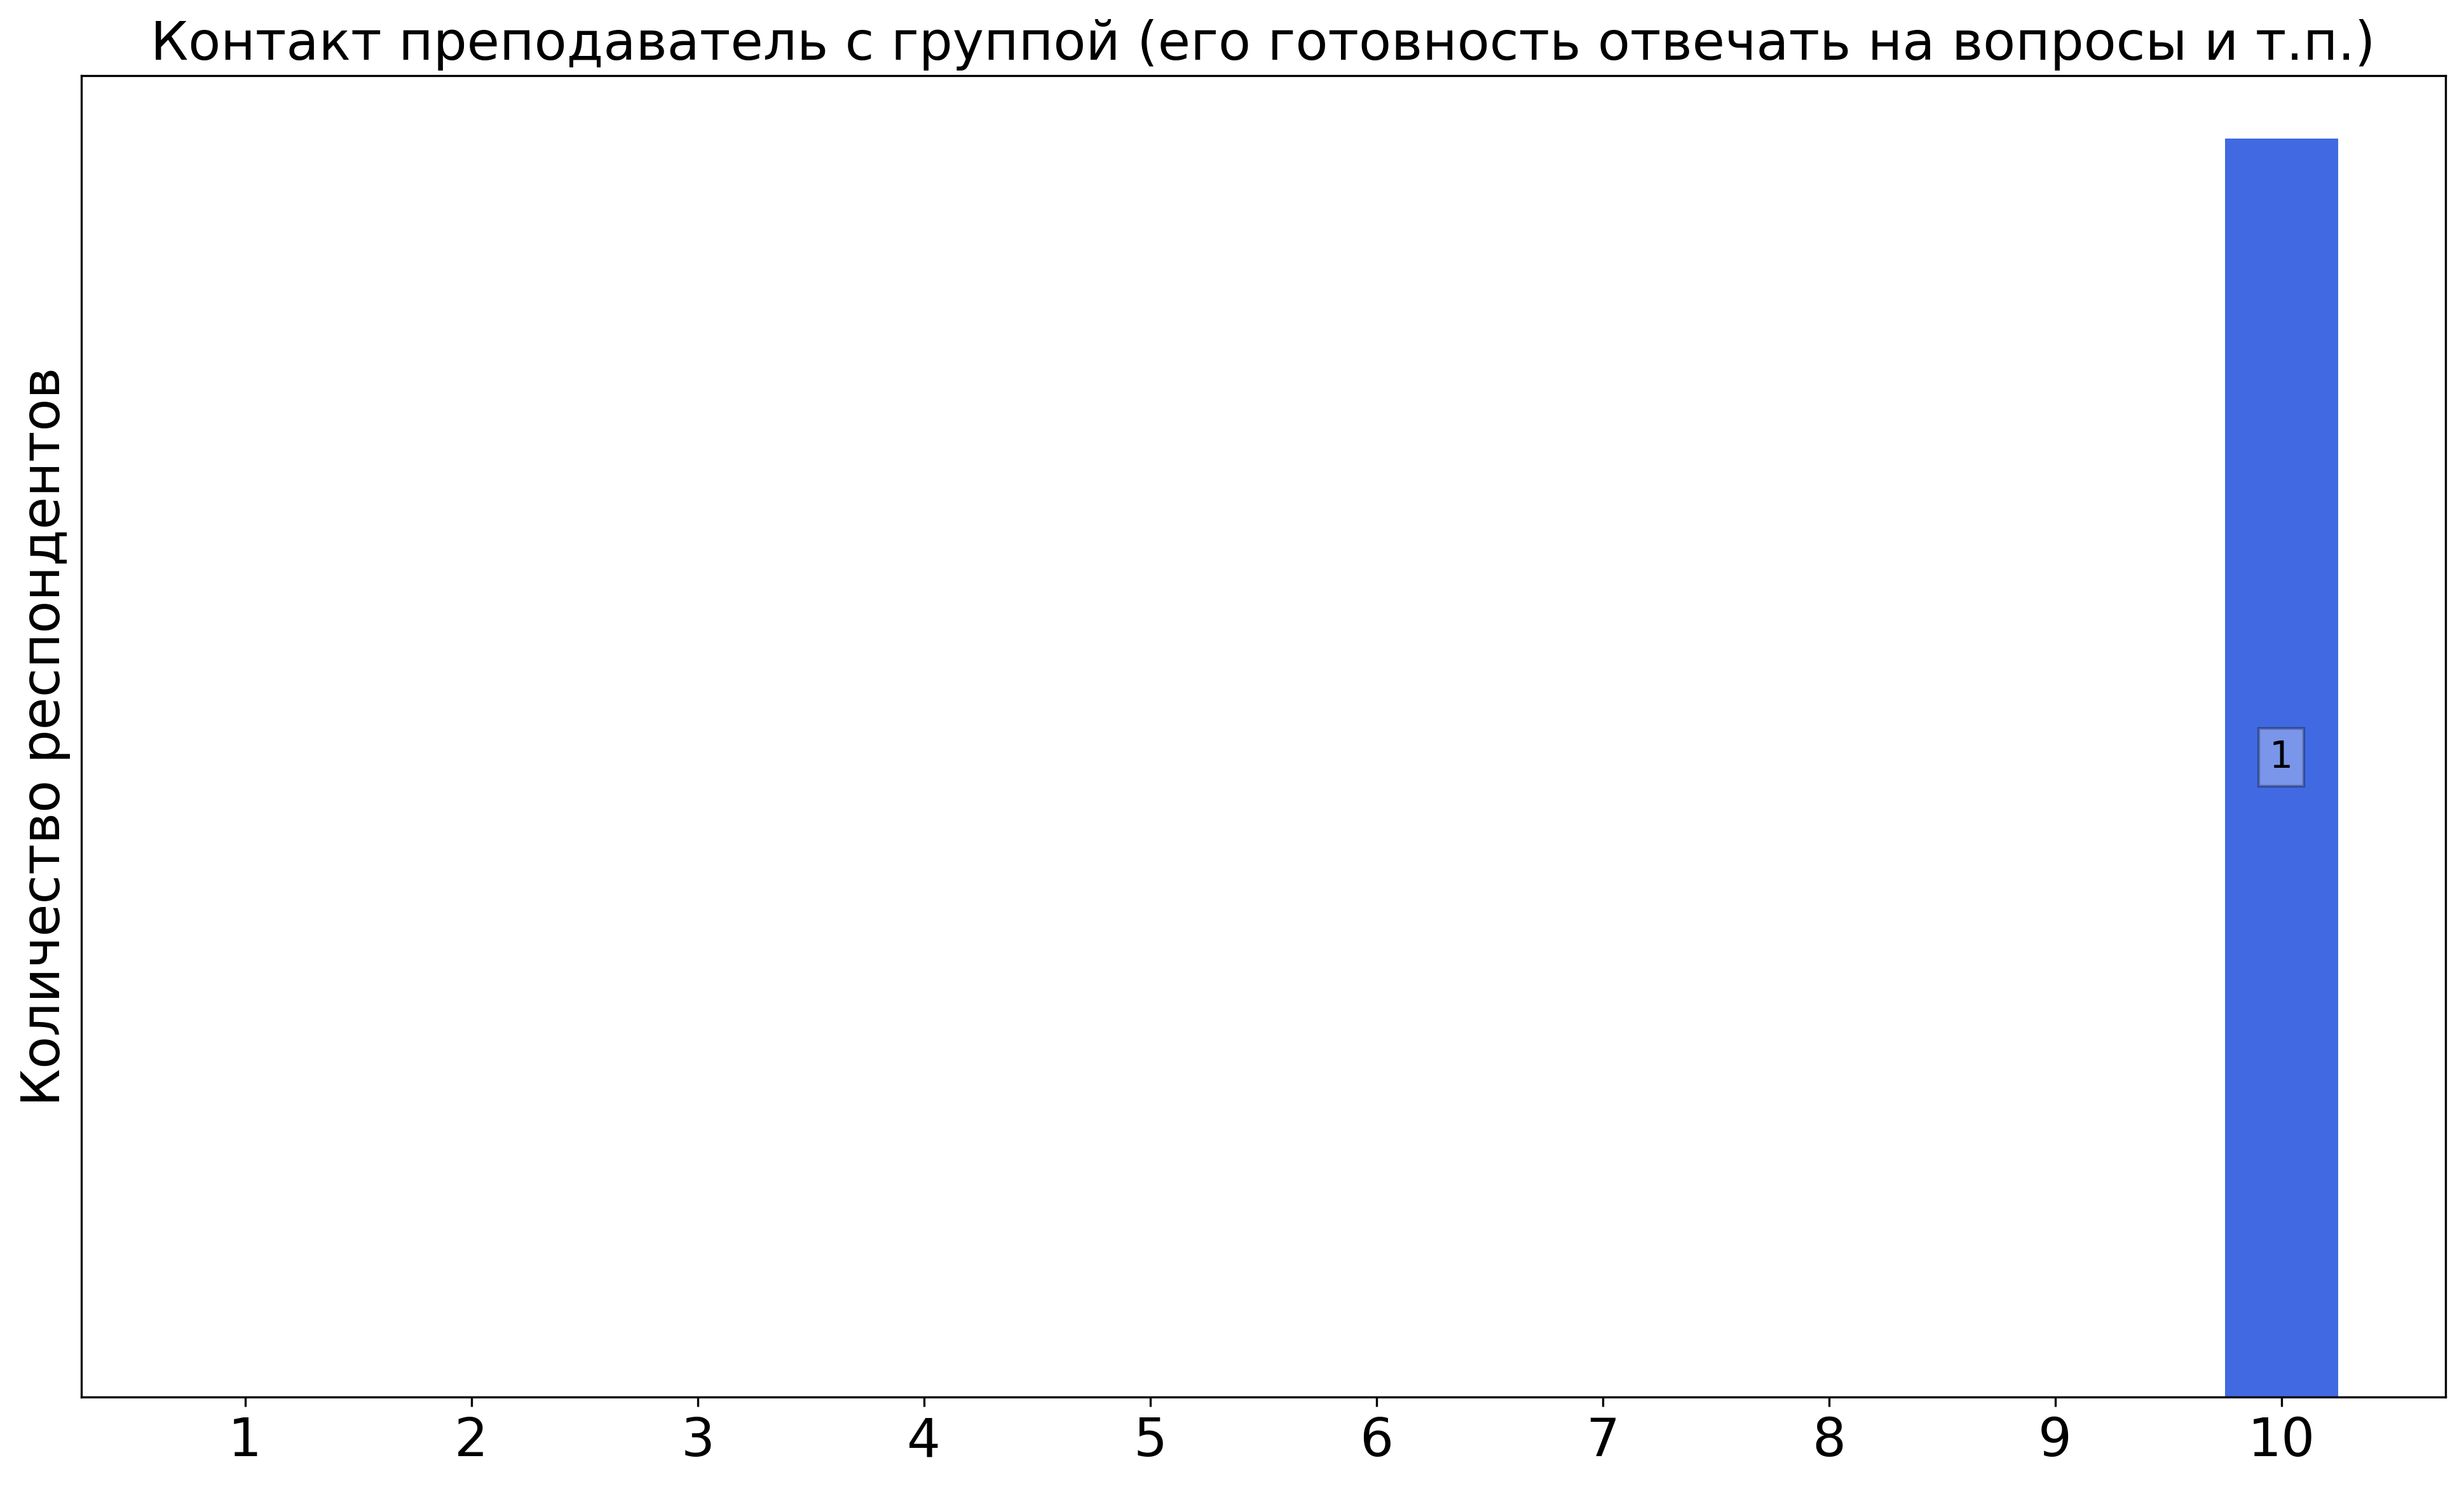
\includegraphics[width=\textwidth]{images/2 course/Радиотехнические цепи и сигналы/labniks-marks-Неешпапа А.В.-0.png}
            \end{subfigure}
            \begin{subfigure}[b]{0.45\textwidth}
                \centering
                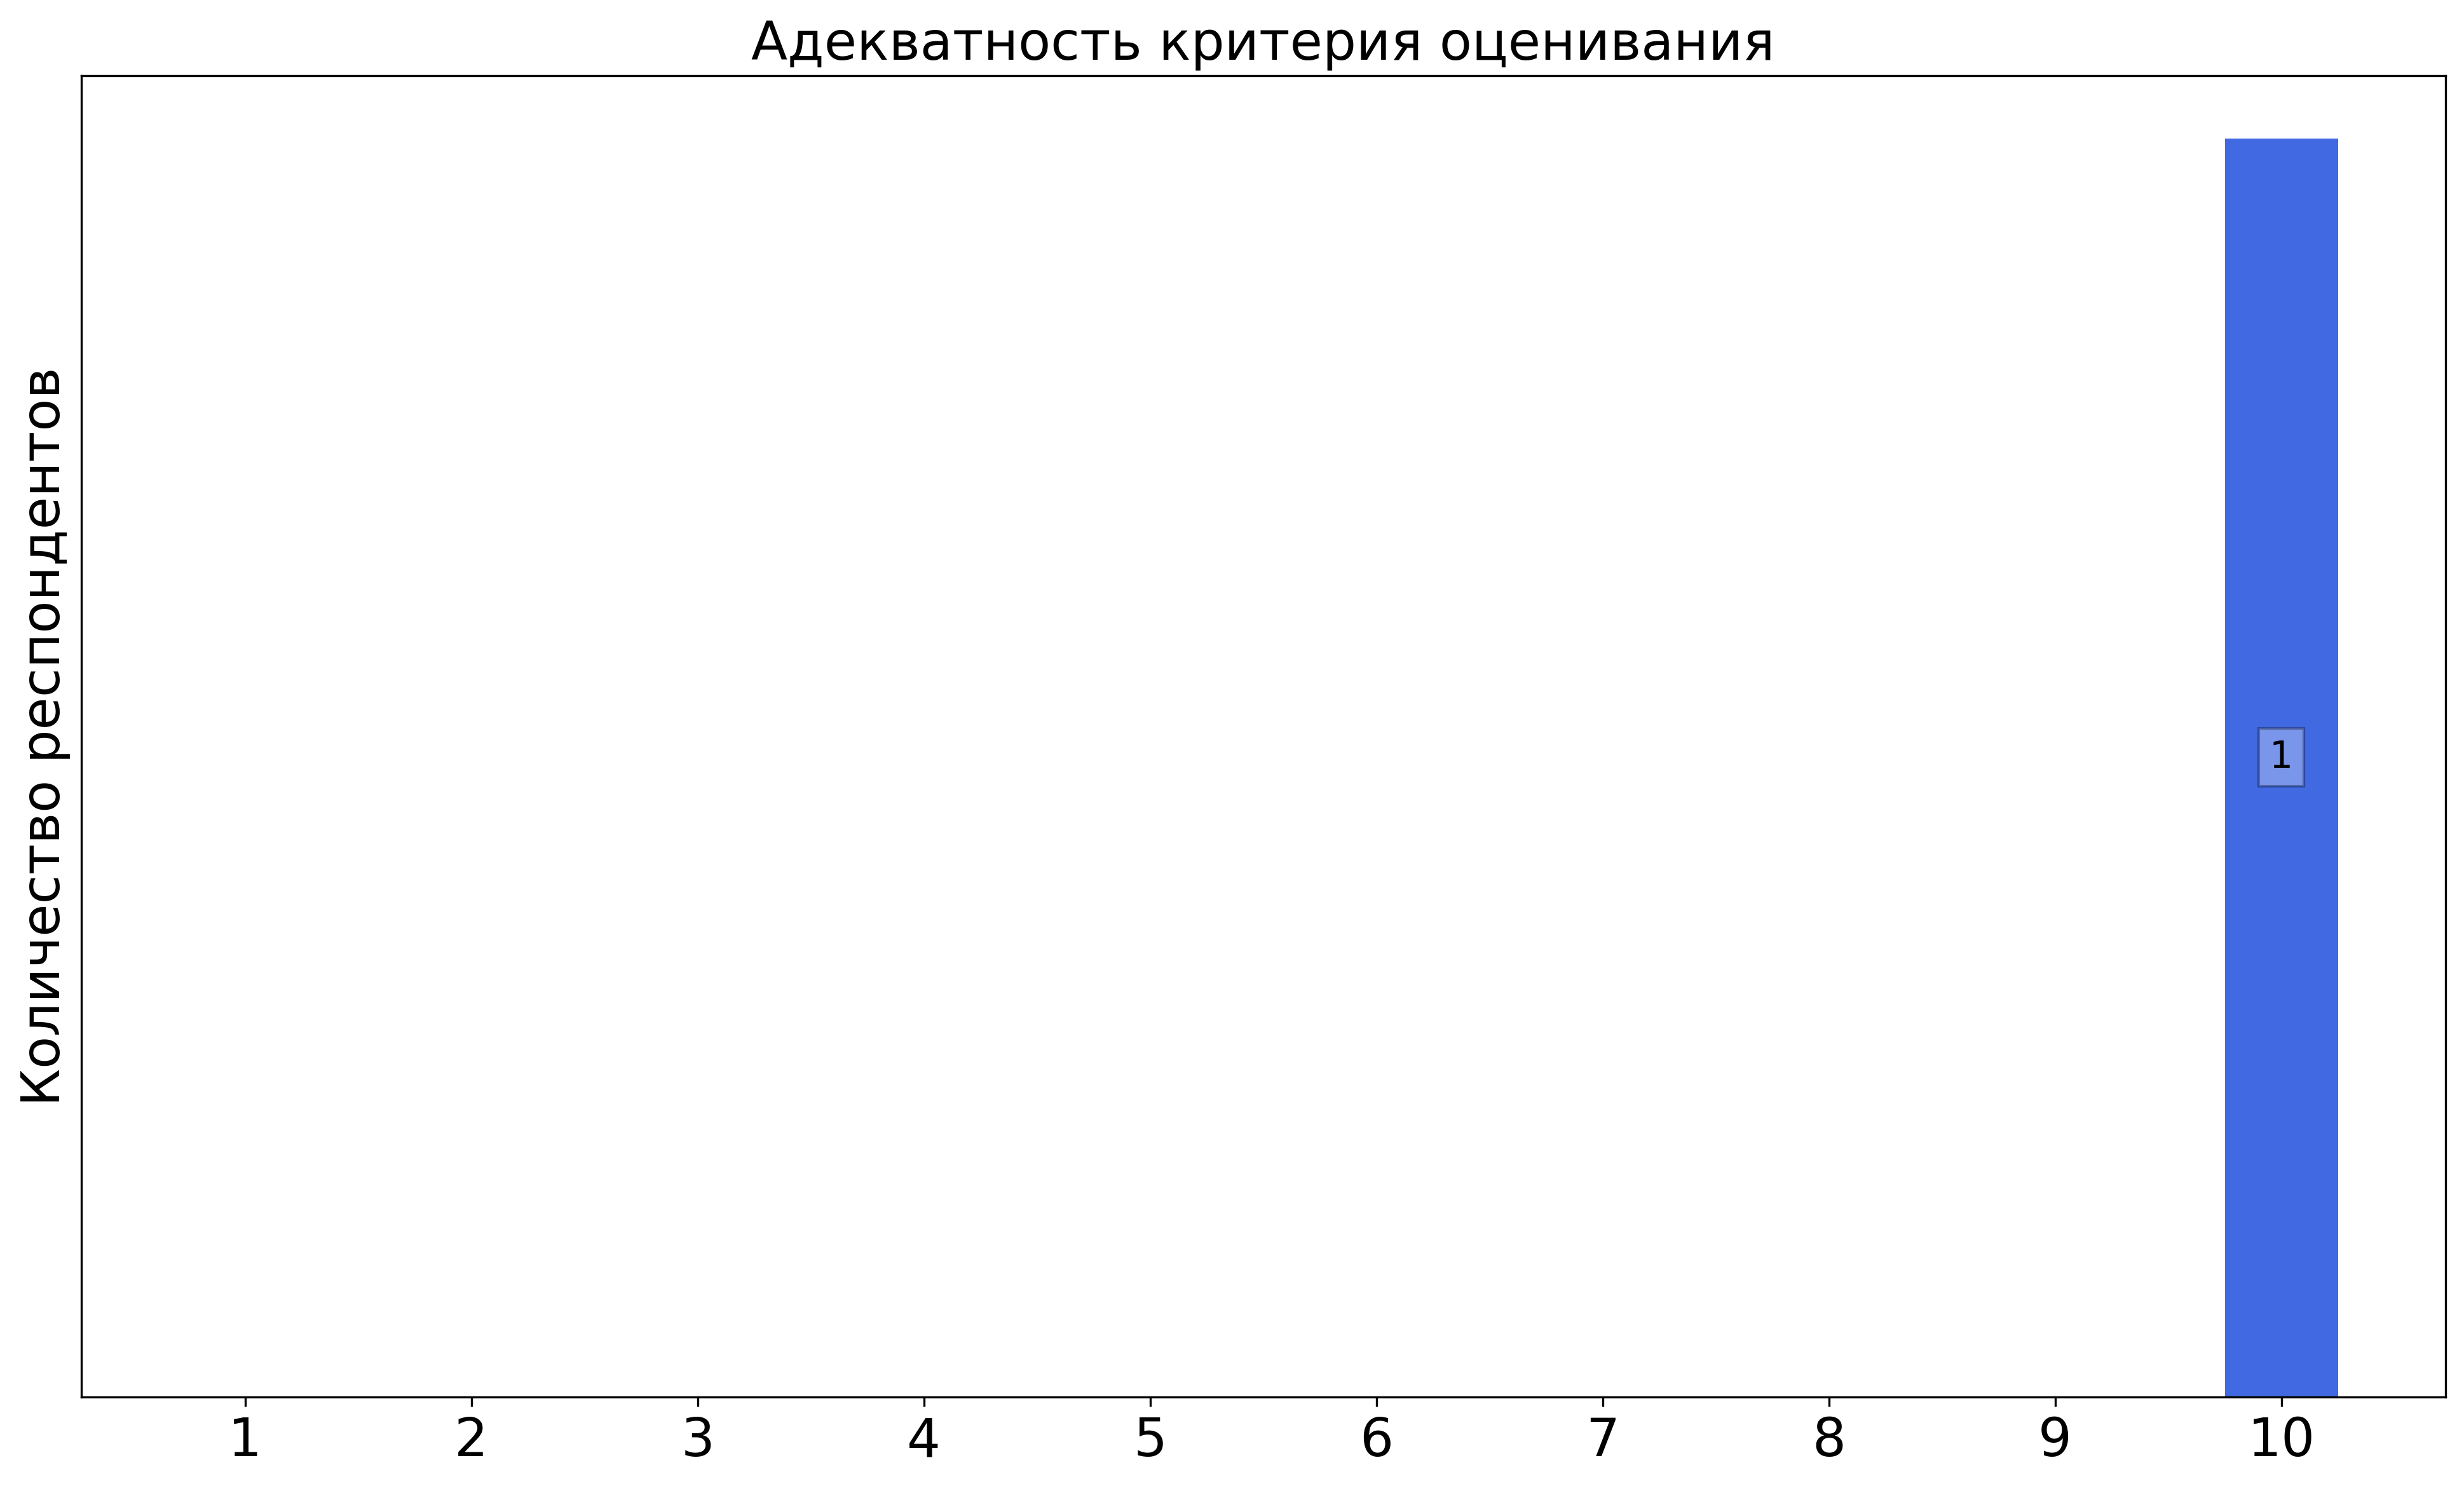
\includegraphics[width=\textwidth]{images/2 course/Радиотехнические цепи и сигналы/labniks-marks-Неешпапа А.В.-1.png}
            \end{subfigure}
            \begin{subfigure}[b]{0.45\textwidth}
                \centering
                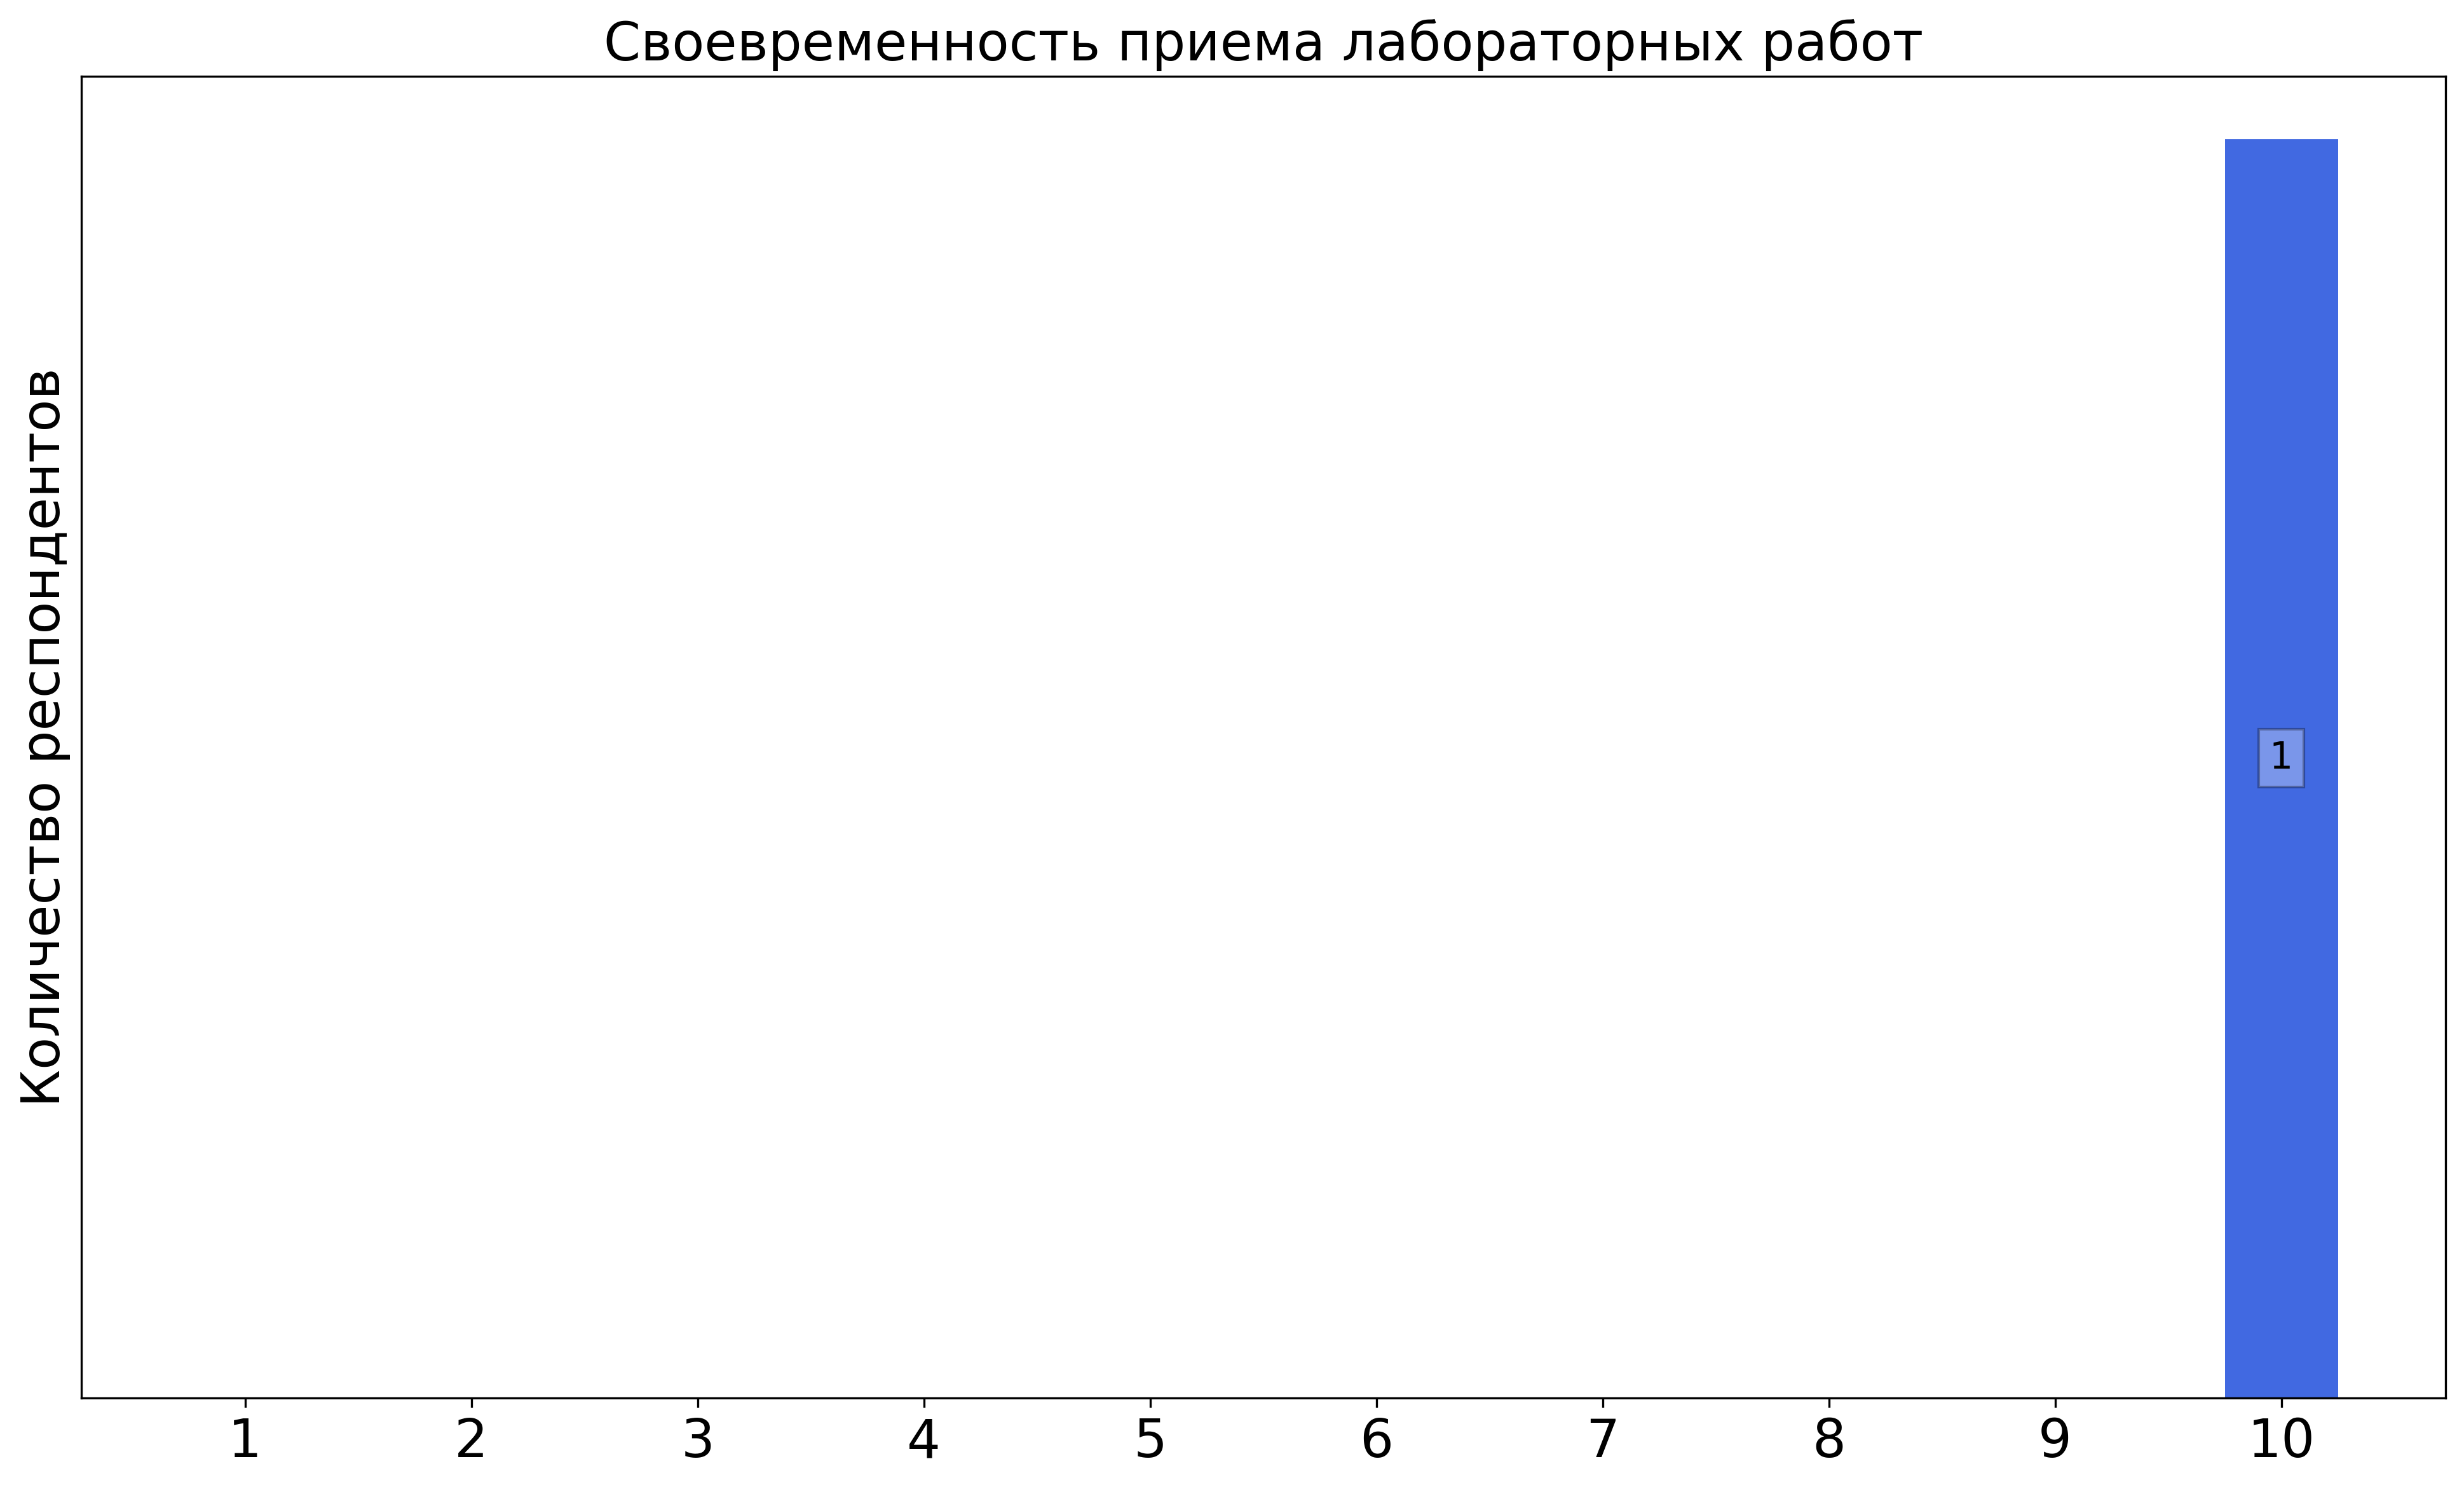
\includegraphics[width=\textwidth]{images/2 course/Радиотехнические цепи и сигналы/labniks-marks-Неешпапа А.В.-2.png}
            \end{subfigure}
            \begin{subfigure}[b]{0.45\textwidth}
                \centering
                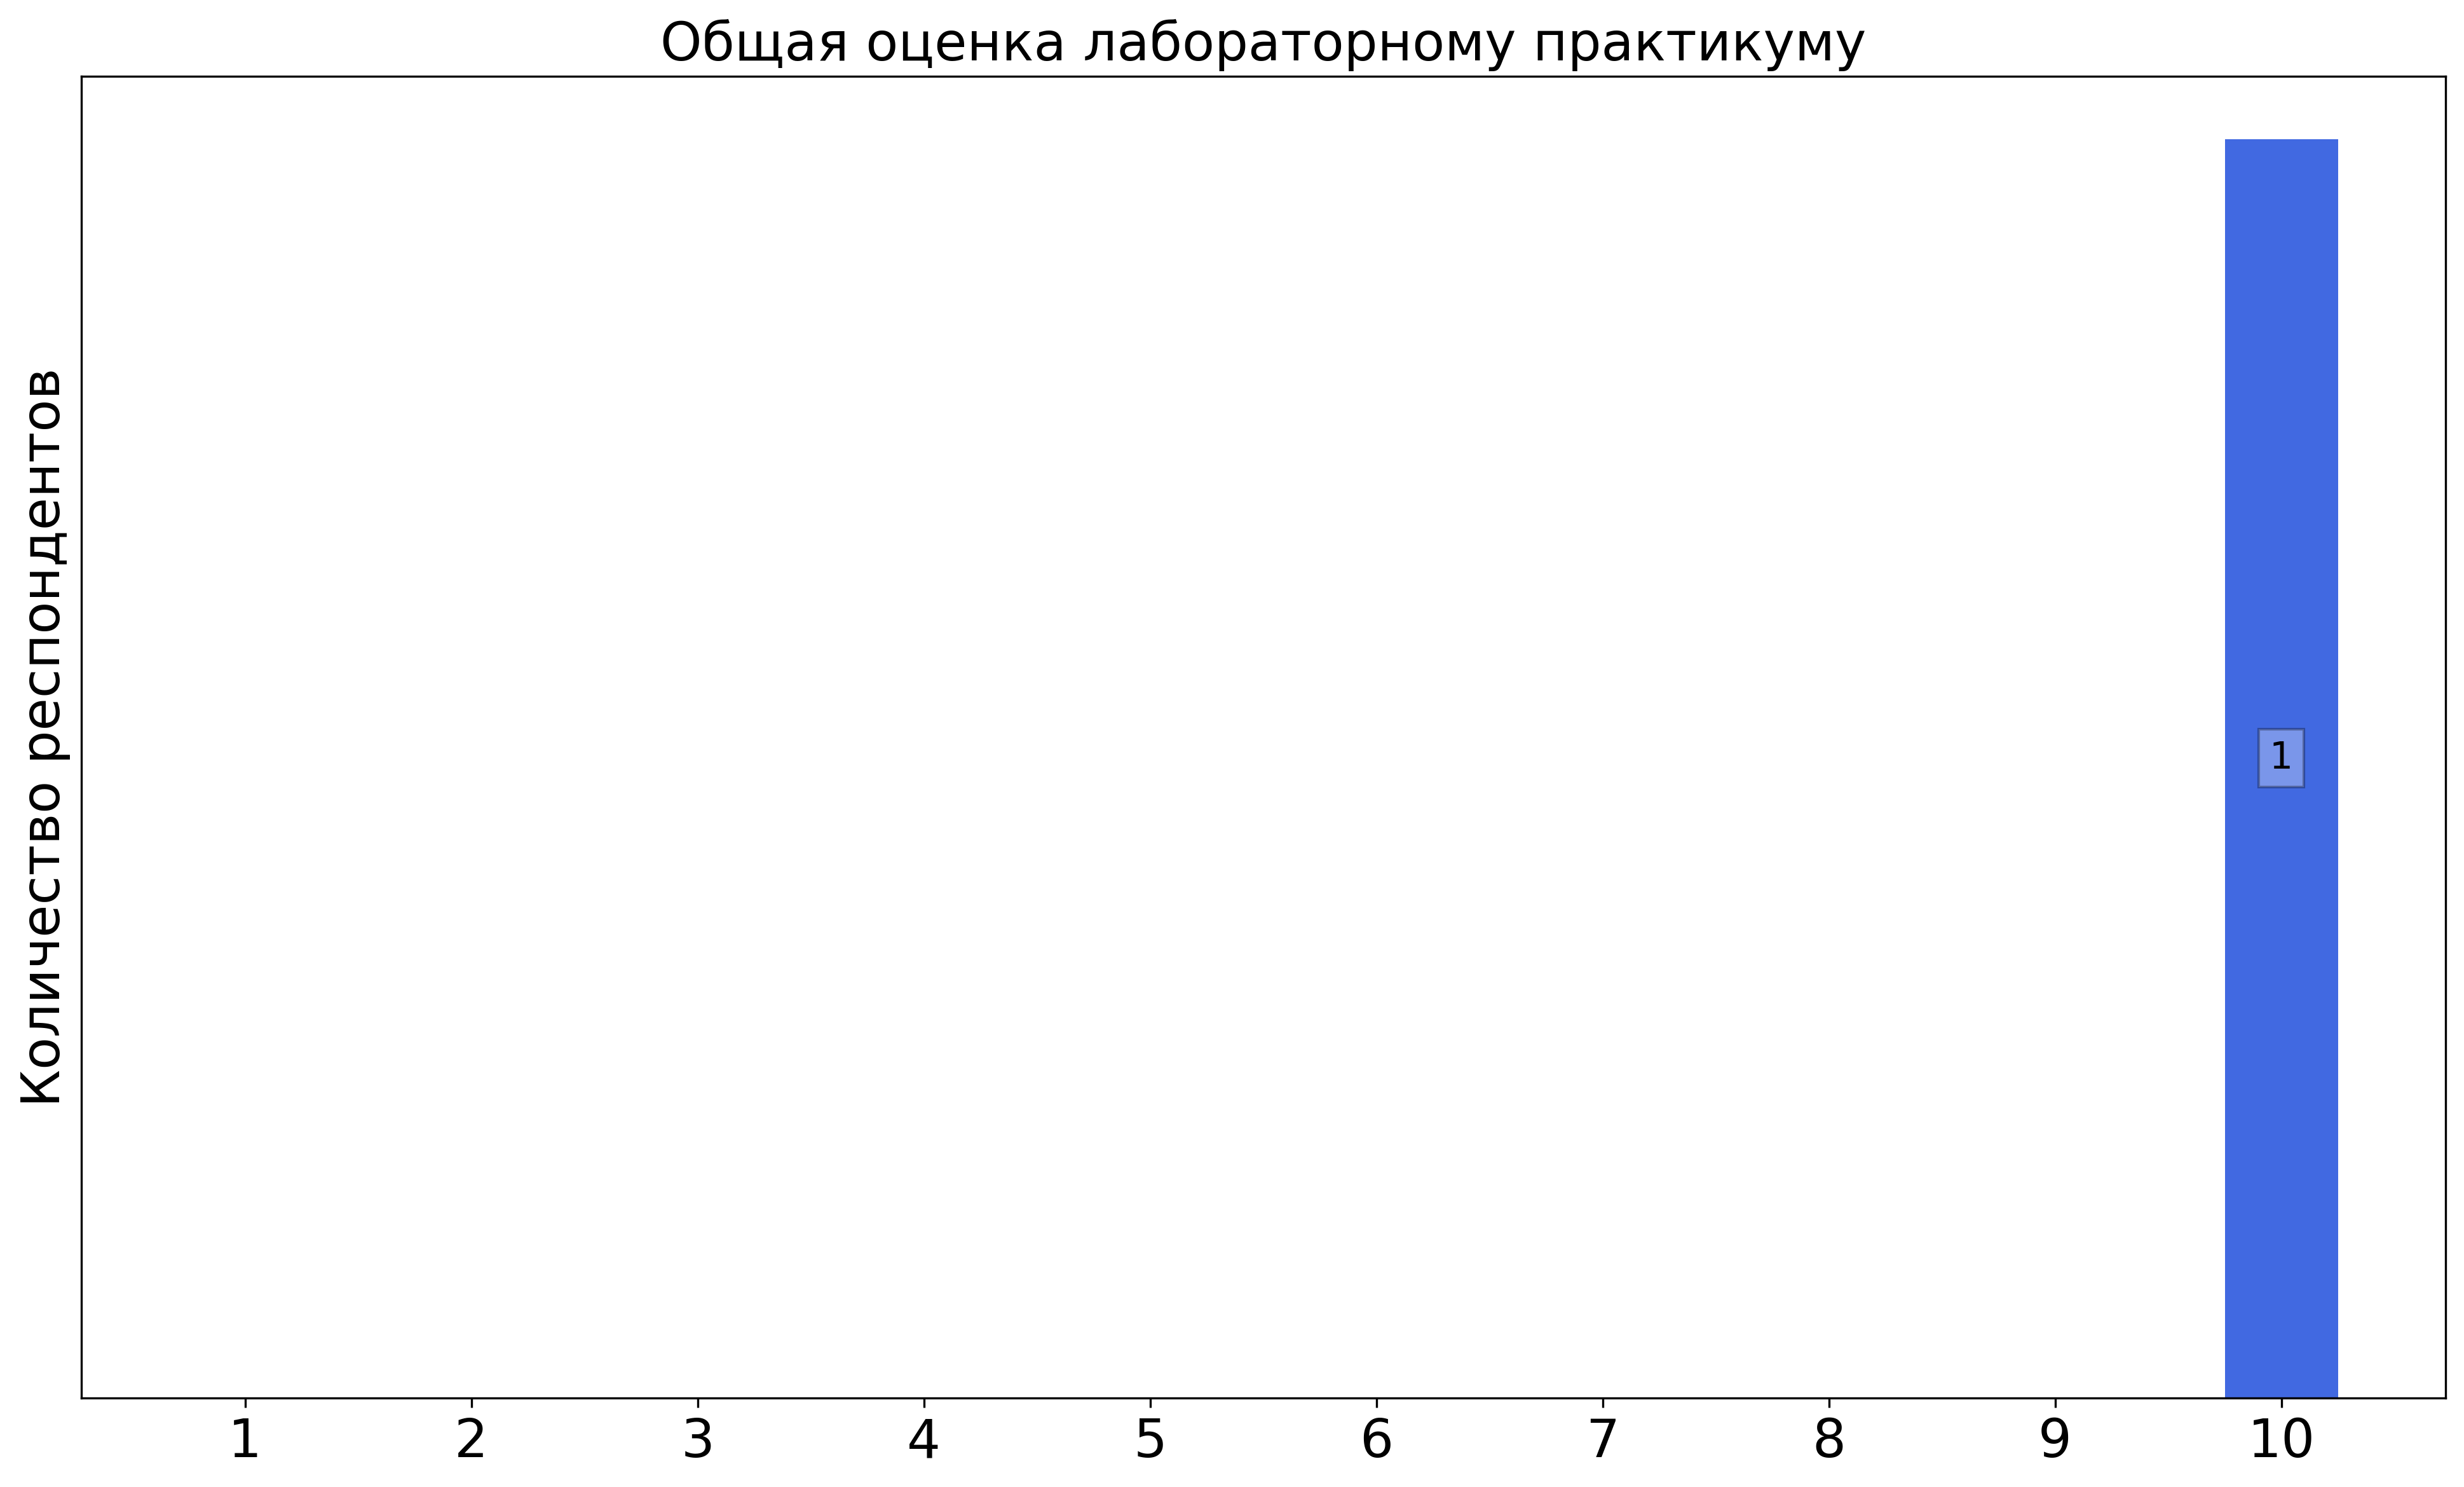
\includegraphics[width=\textwidth]{images/2 course/Радиотехнические цепи и сигналы/labniks-marks-Неешпапа А.В.-3.png}
            \end{subfigure}	
            \caption{Оценки респондентов о качестве преподавания лабораторных работ}
        \end{figure}


        
    \subsubsection{Отзыв студентов о лабораторных работах. Преподаватель: Скурихин А.В.}
        \begin{figure}[H]
            \centering
            \begin{subfigure}[b]{0.45\textwidth}
                \centering
                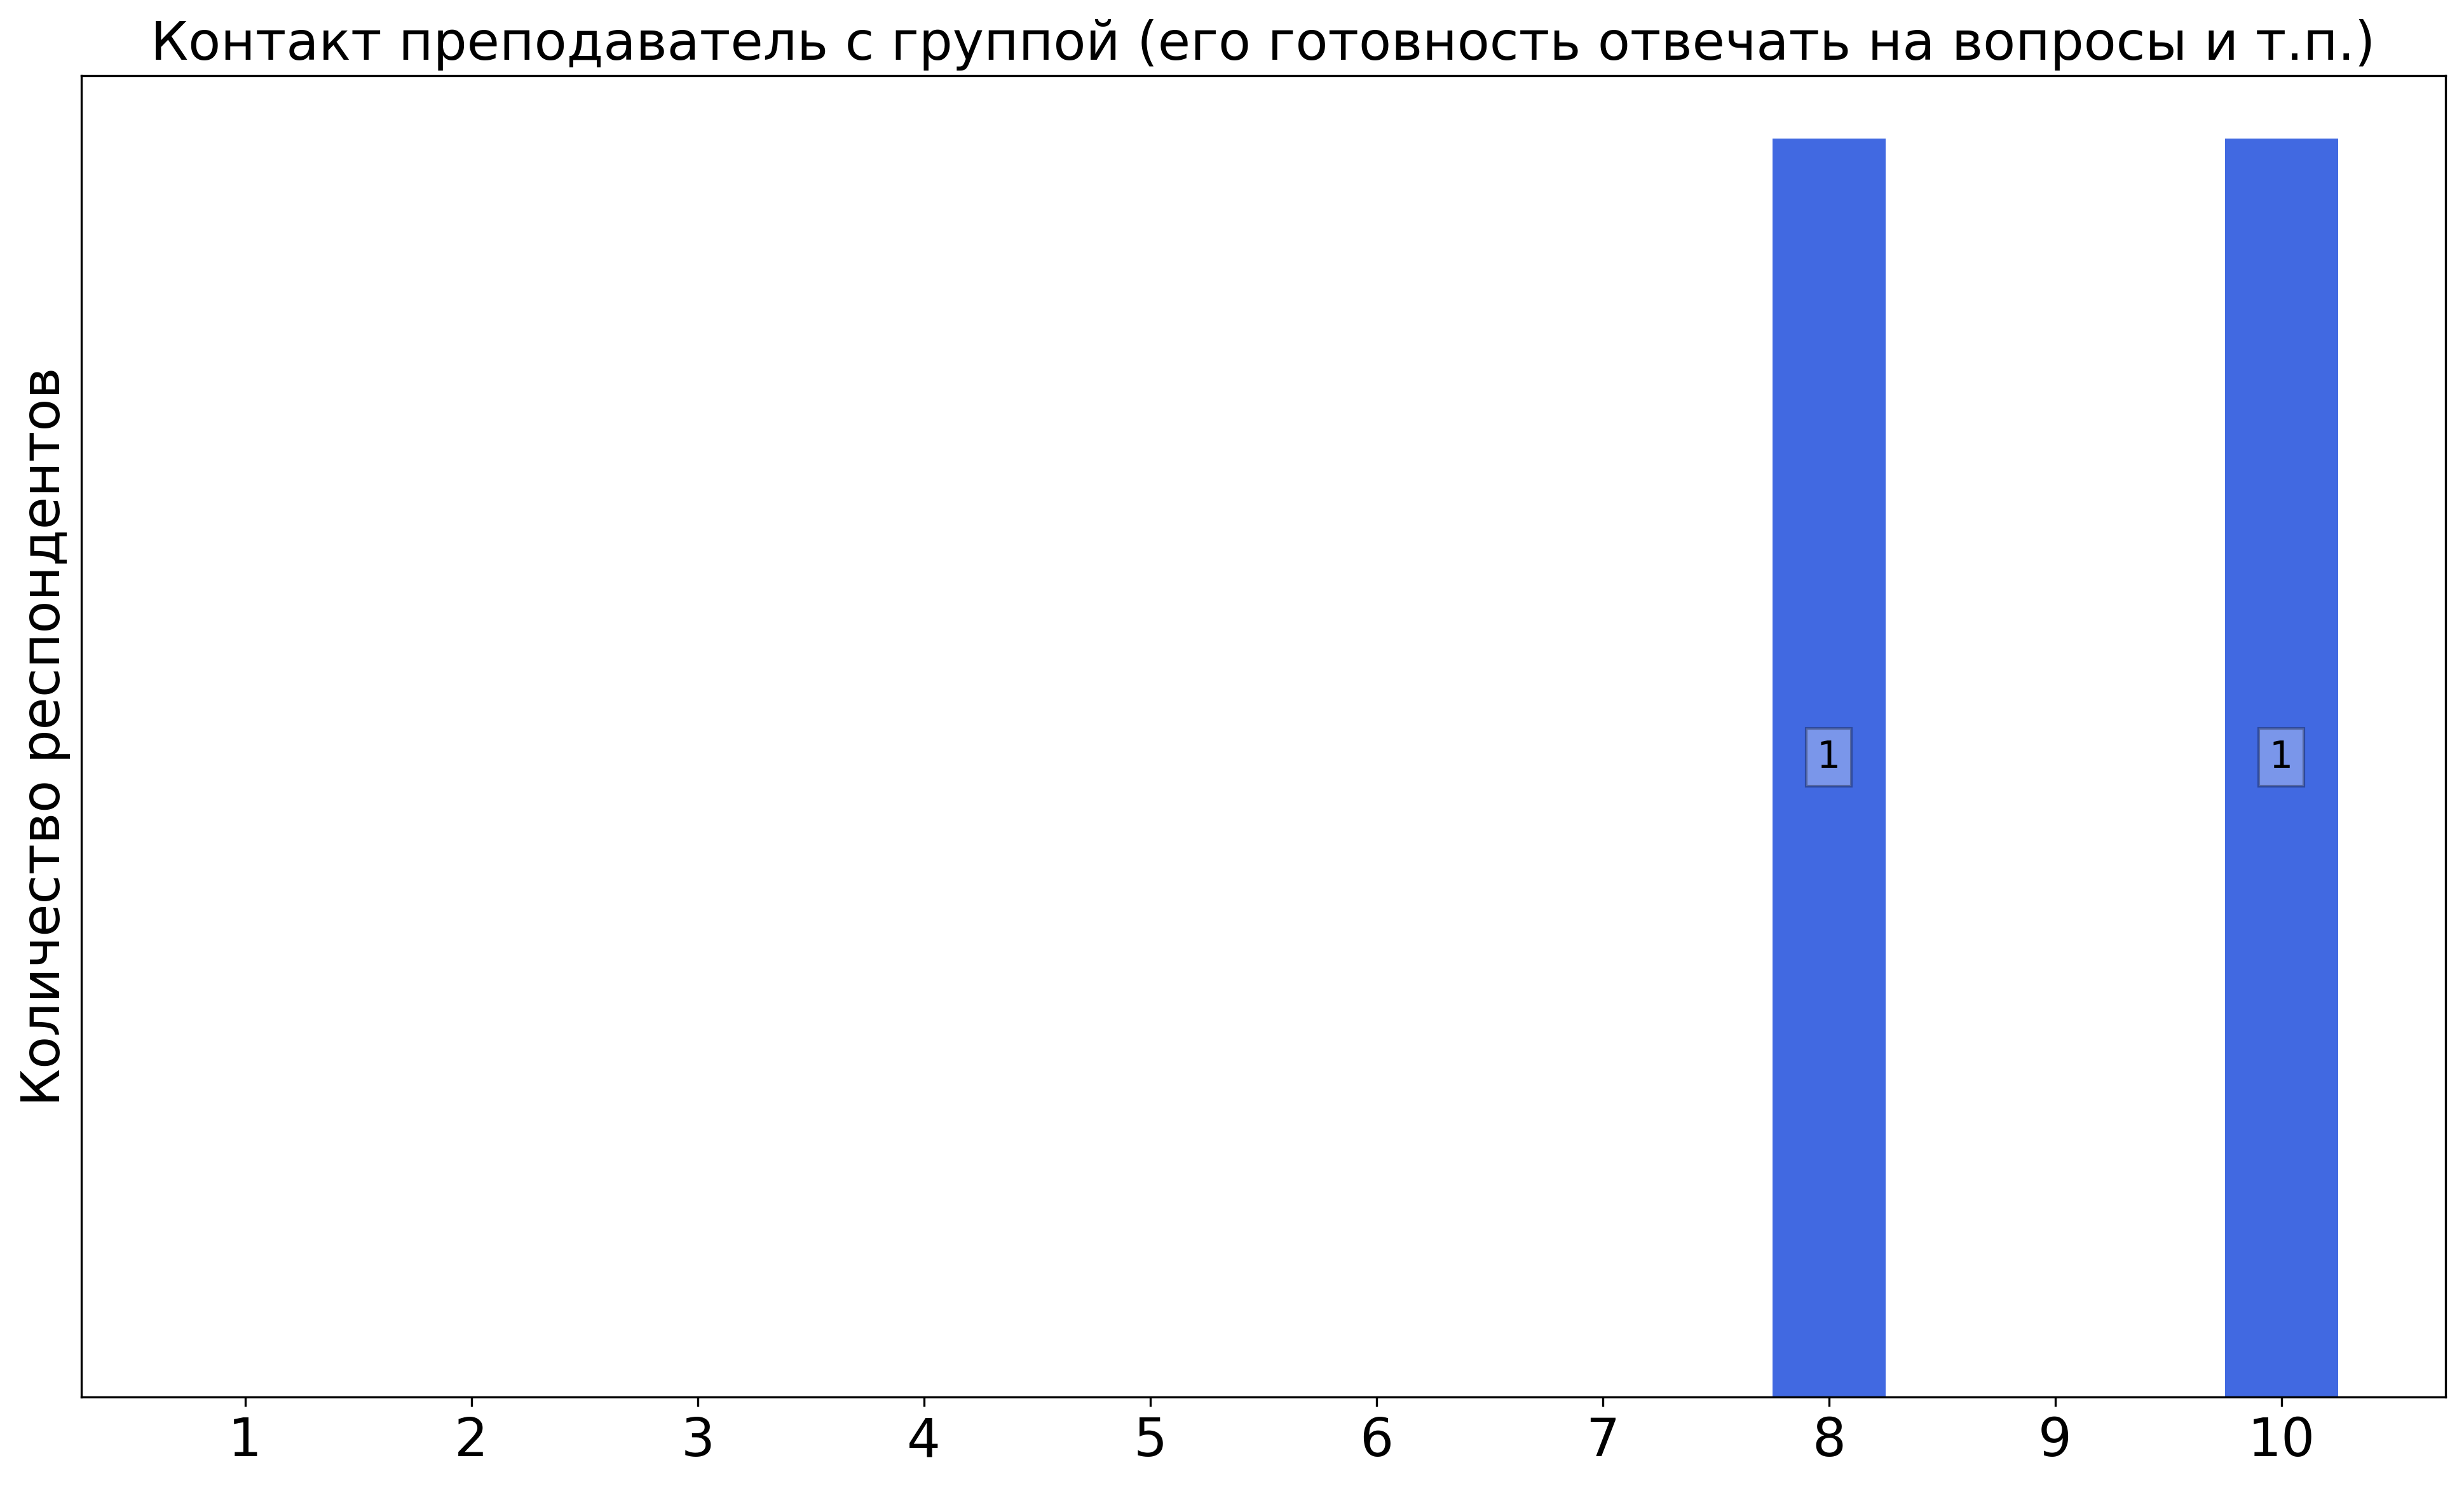
\includegraphics[width=\textwidth]{images/2 course/Радиотехнические цепи и сигналы/labniks-marks-Скурихин А.В.-0.png}
            \end{subfigure}
            \begin{subfigure}[b]{0.45\textwidth}
                \centering
                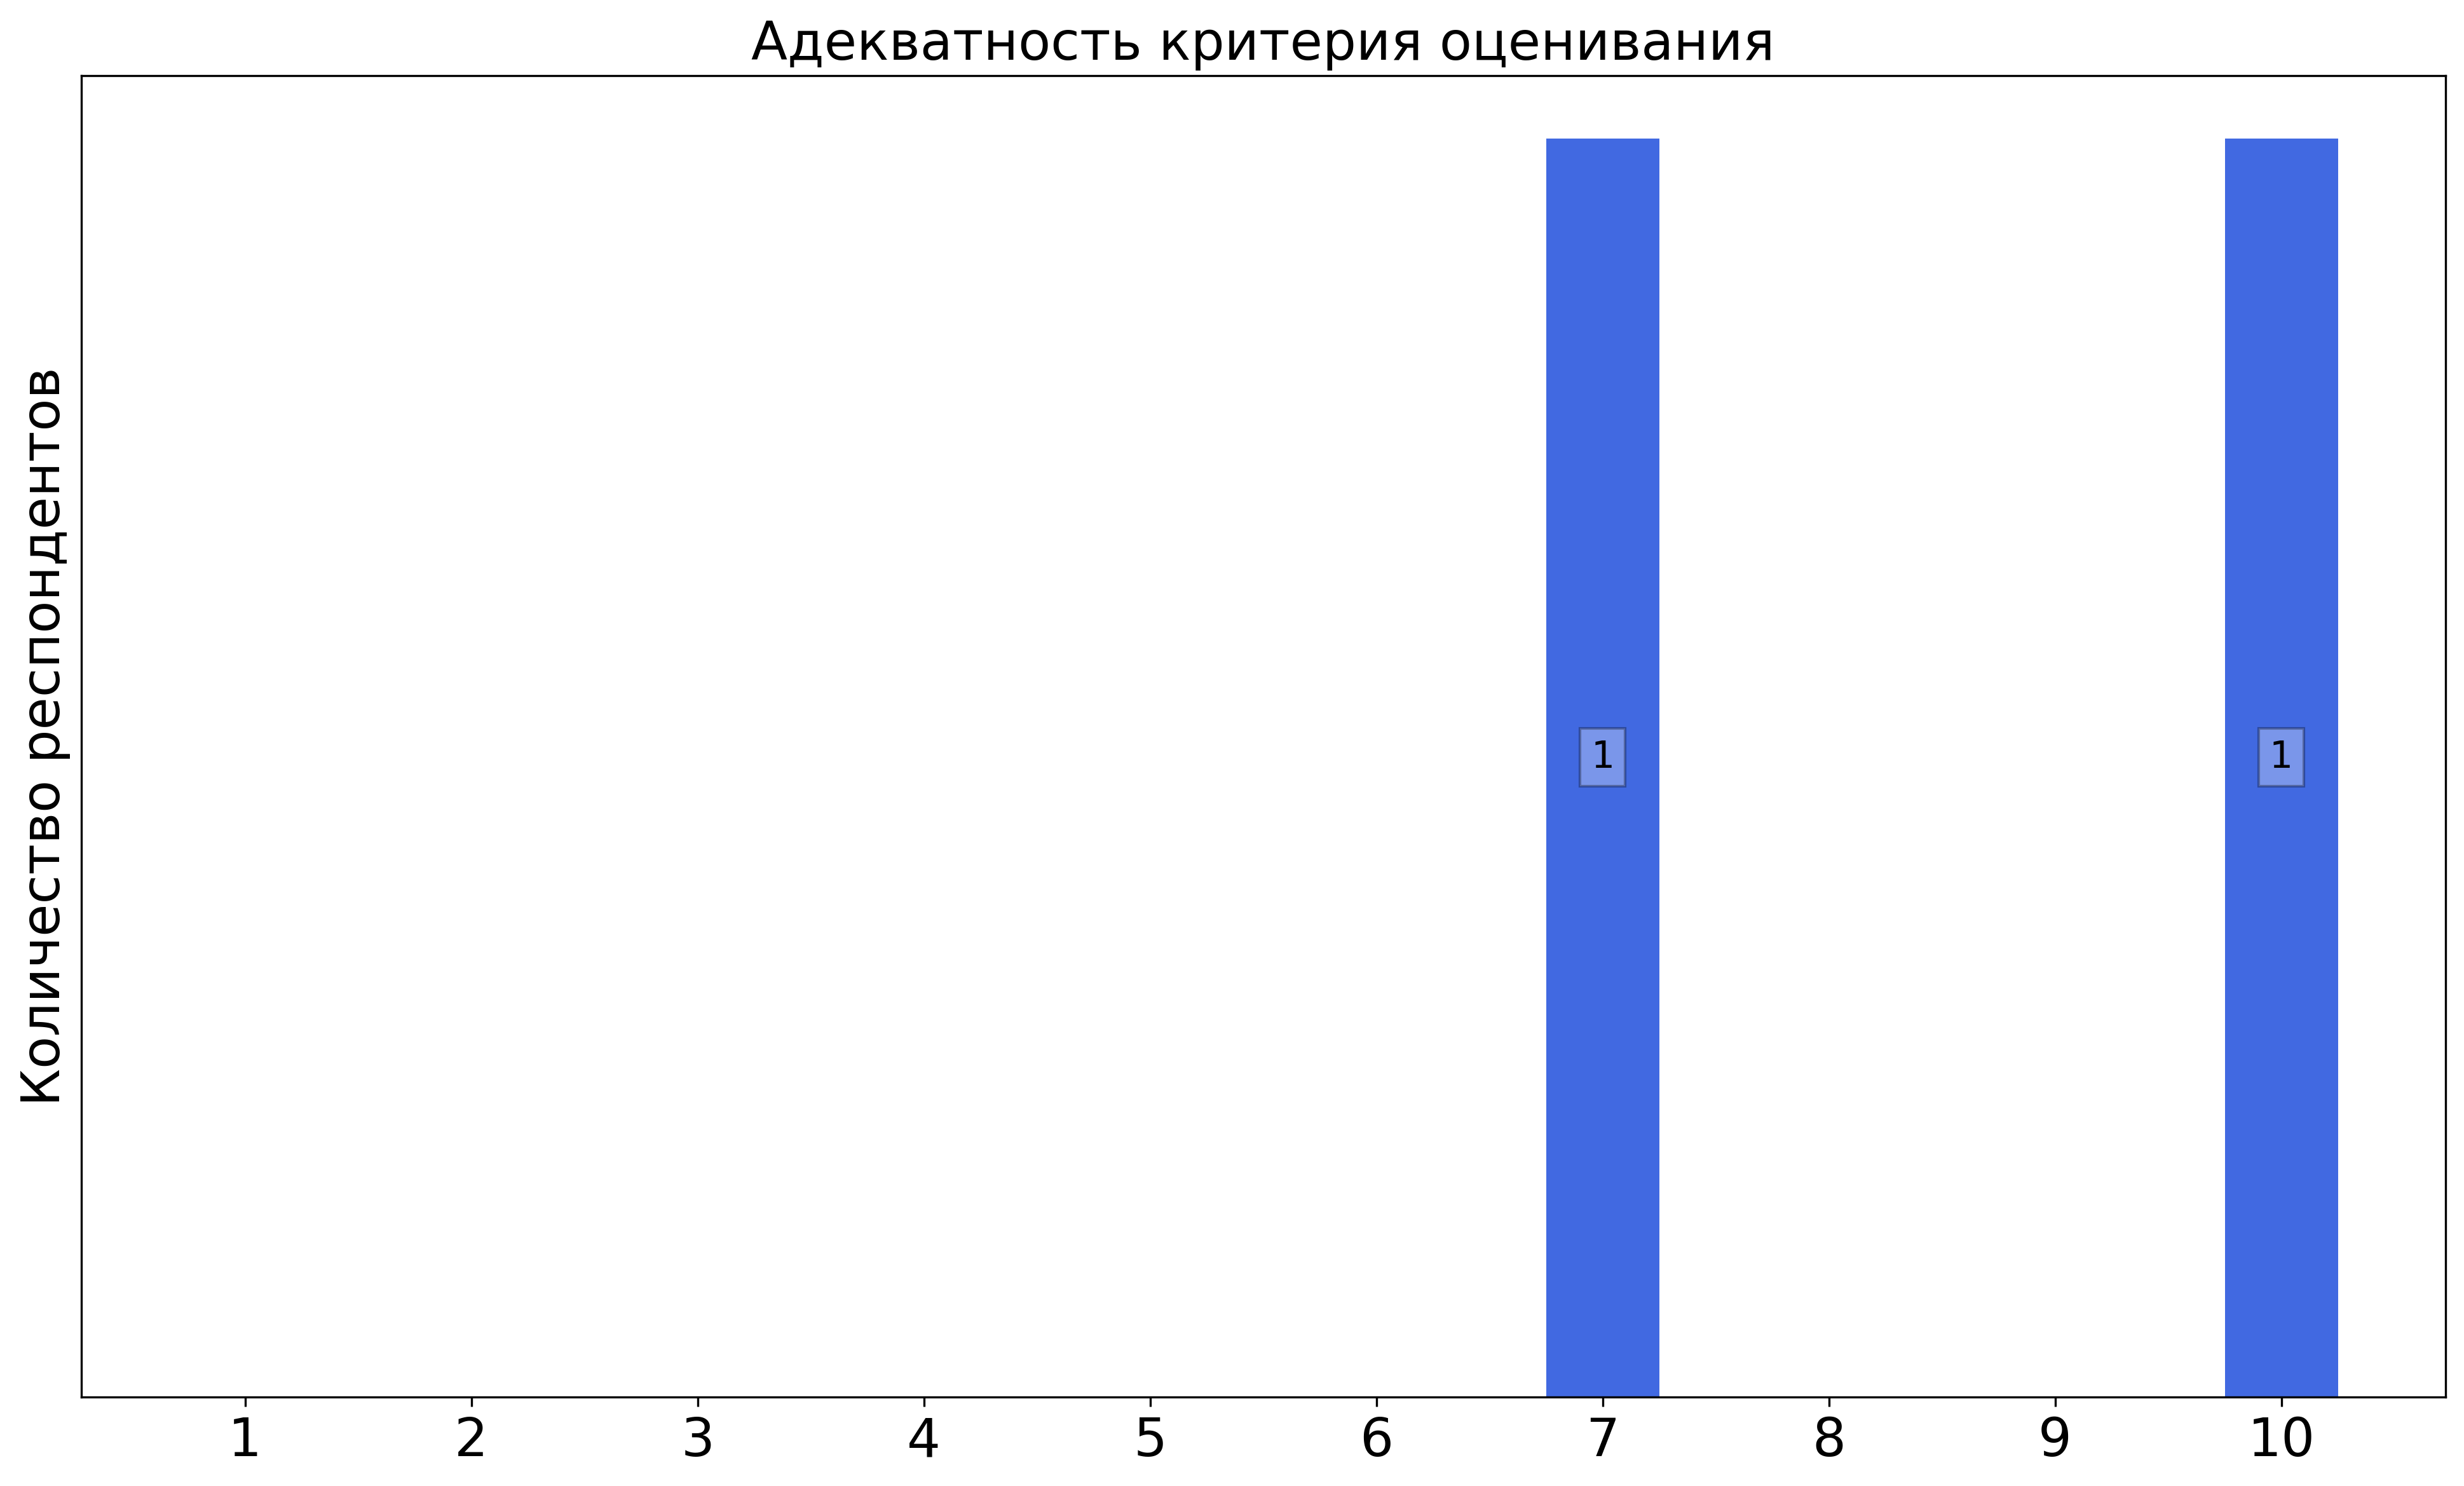
\includegraphics[width=\textwidth]{images/2 course/Радиотехнические цепи и сигналы/labniks-marks-Скурихин А.В.-1.png}
            \end{subfigure}
            \begin{subfigure}[b]{0.45\textwidth}
                \centering
                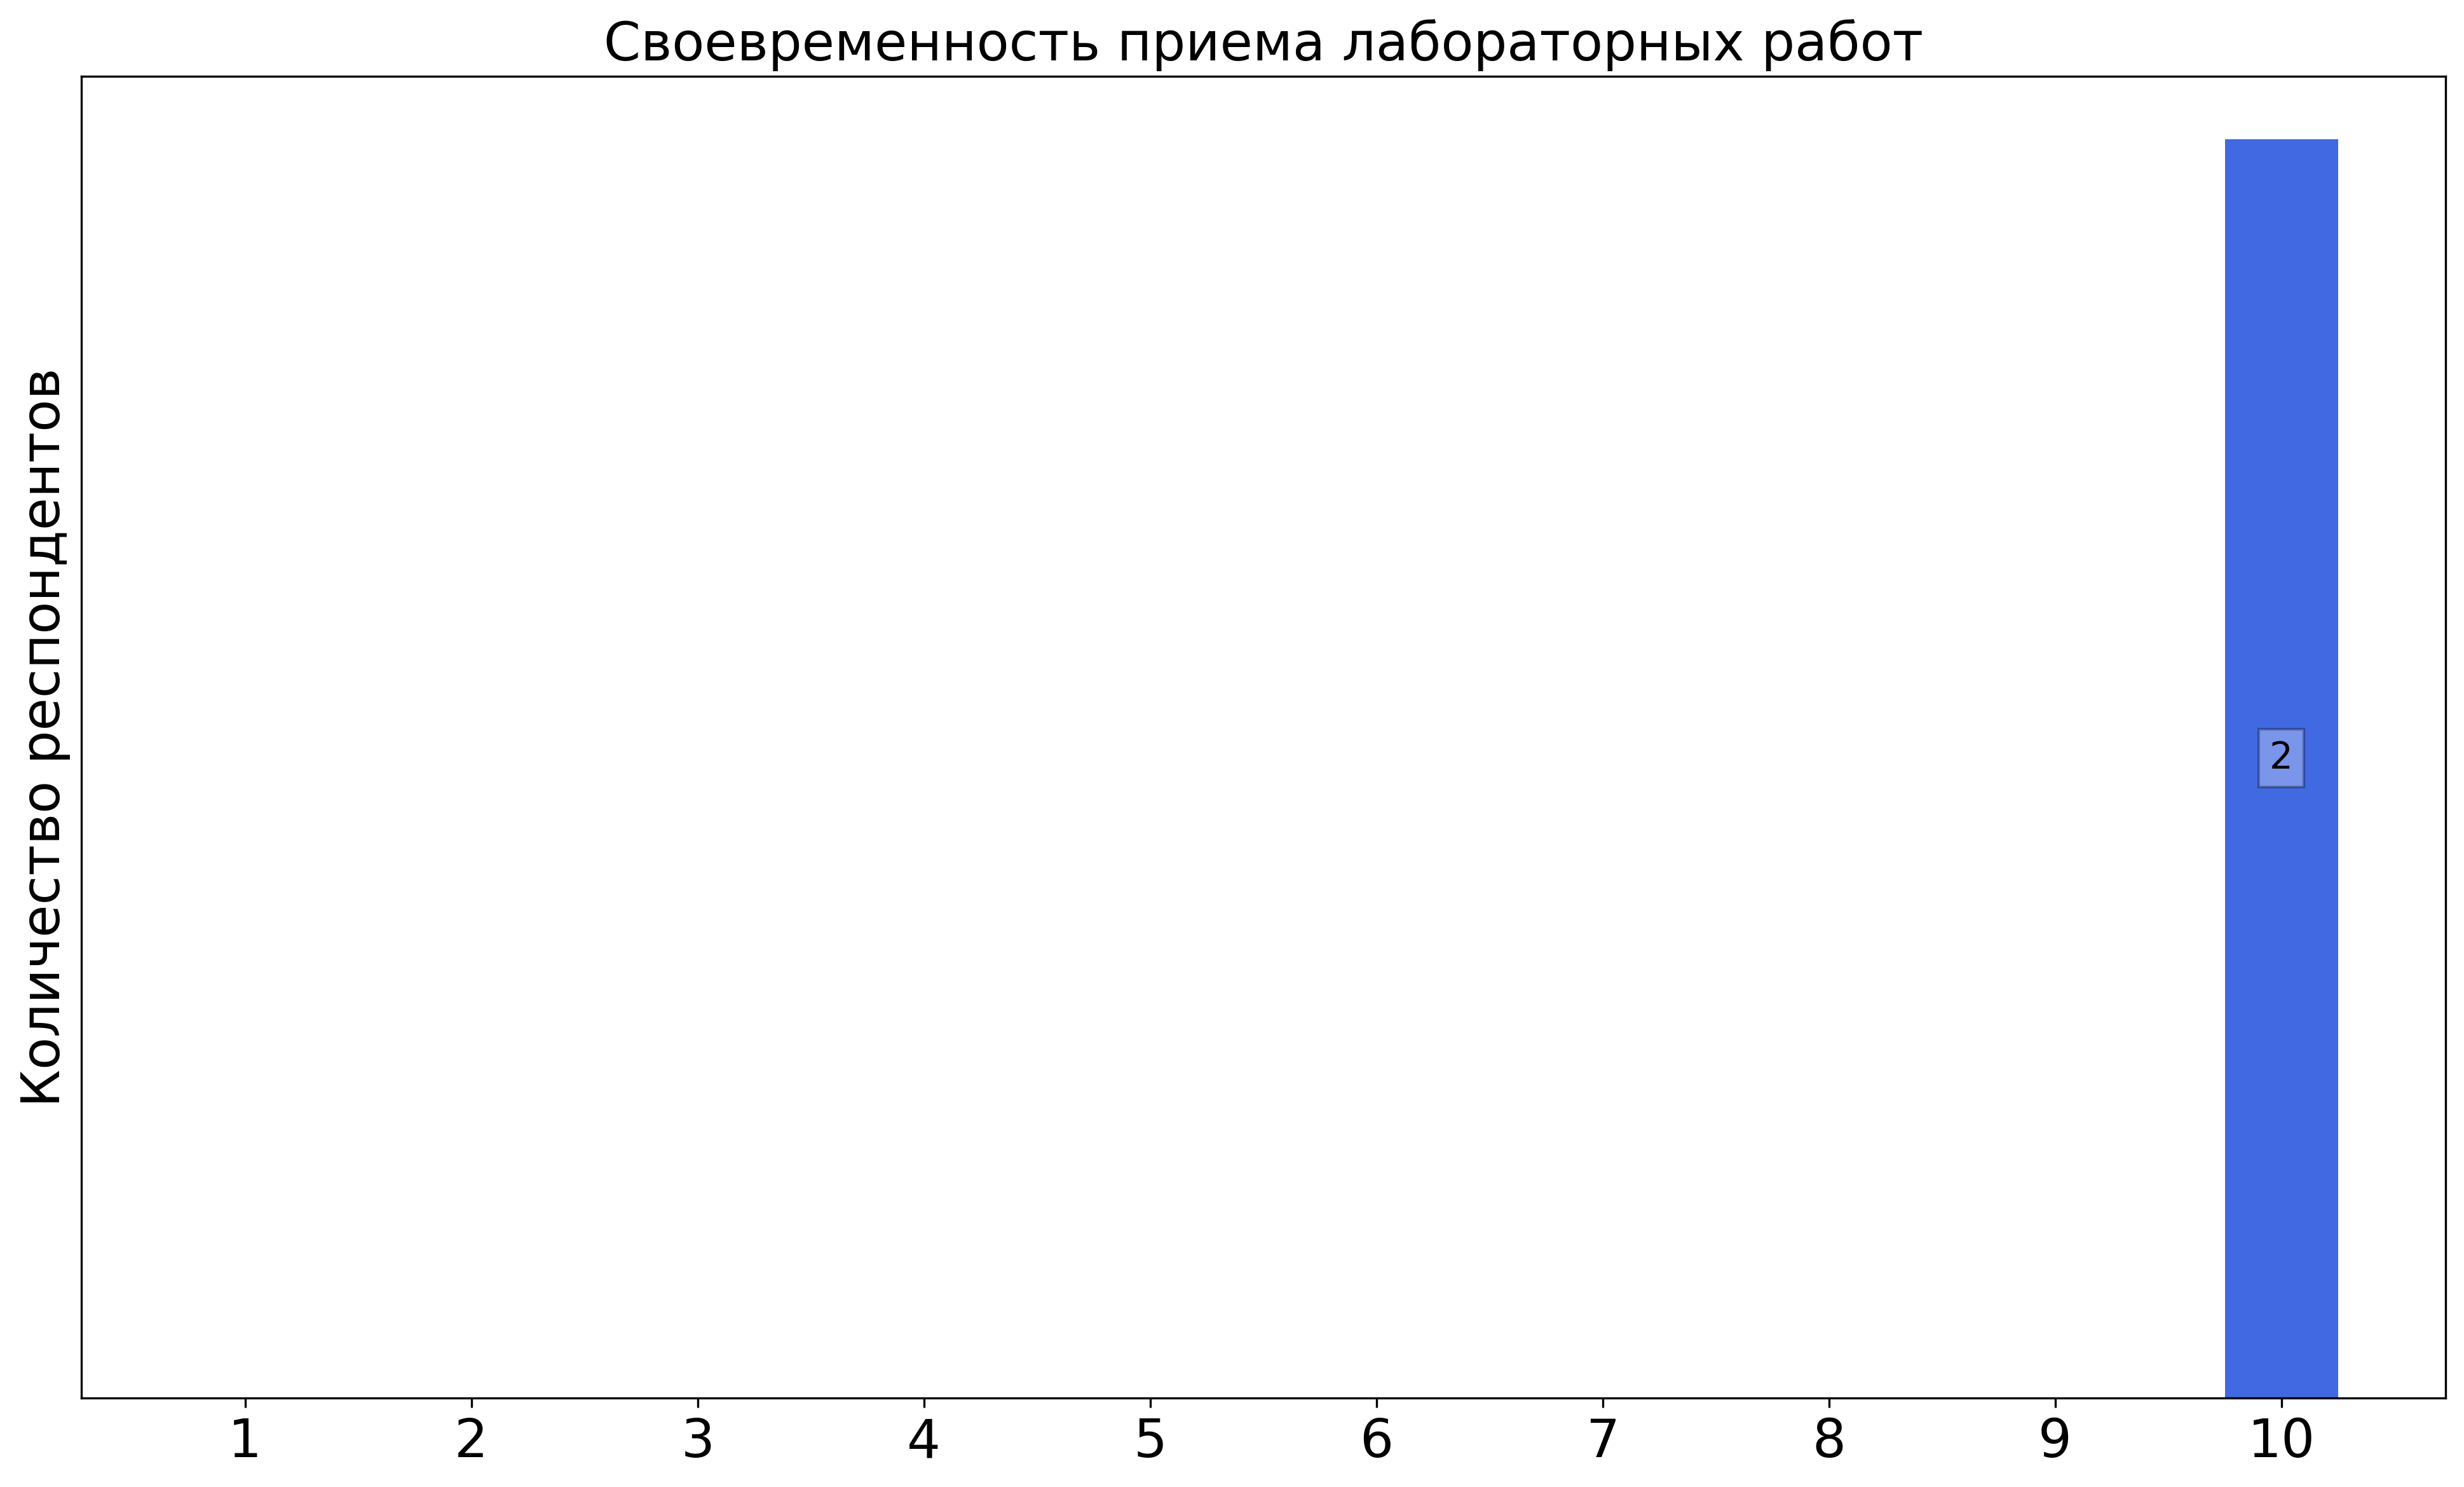
\includegraphics[width=\textwidth]{images/2 course/Радиотехнические цепи и сигналы/labniks-marks-Скурихин А.В.-2.png}
            \end{subfigure}
            \begin{subfigure}[b]{0.45\textwidth}
                \centering
                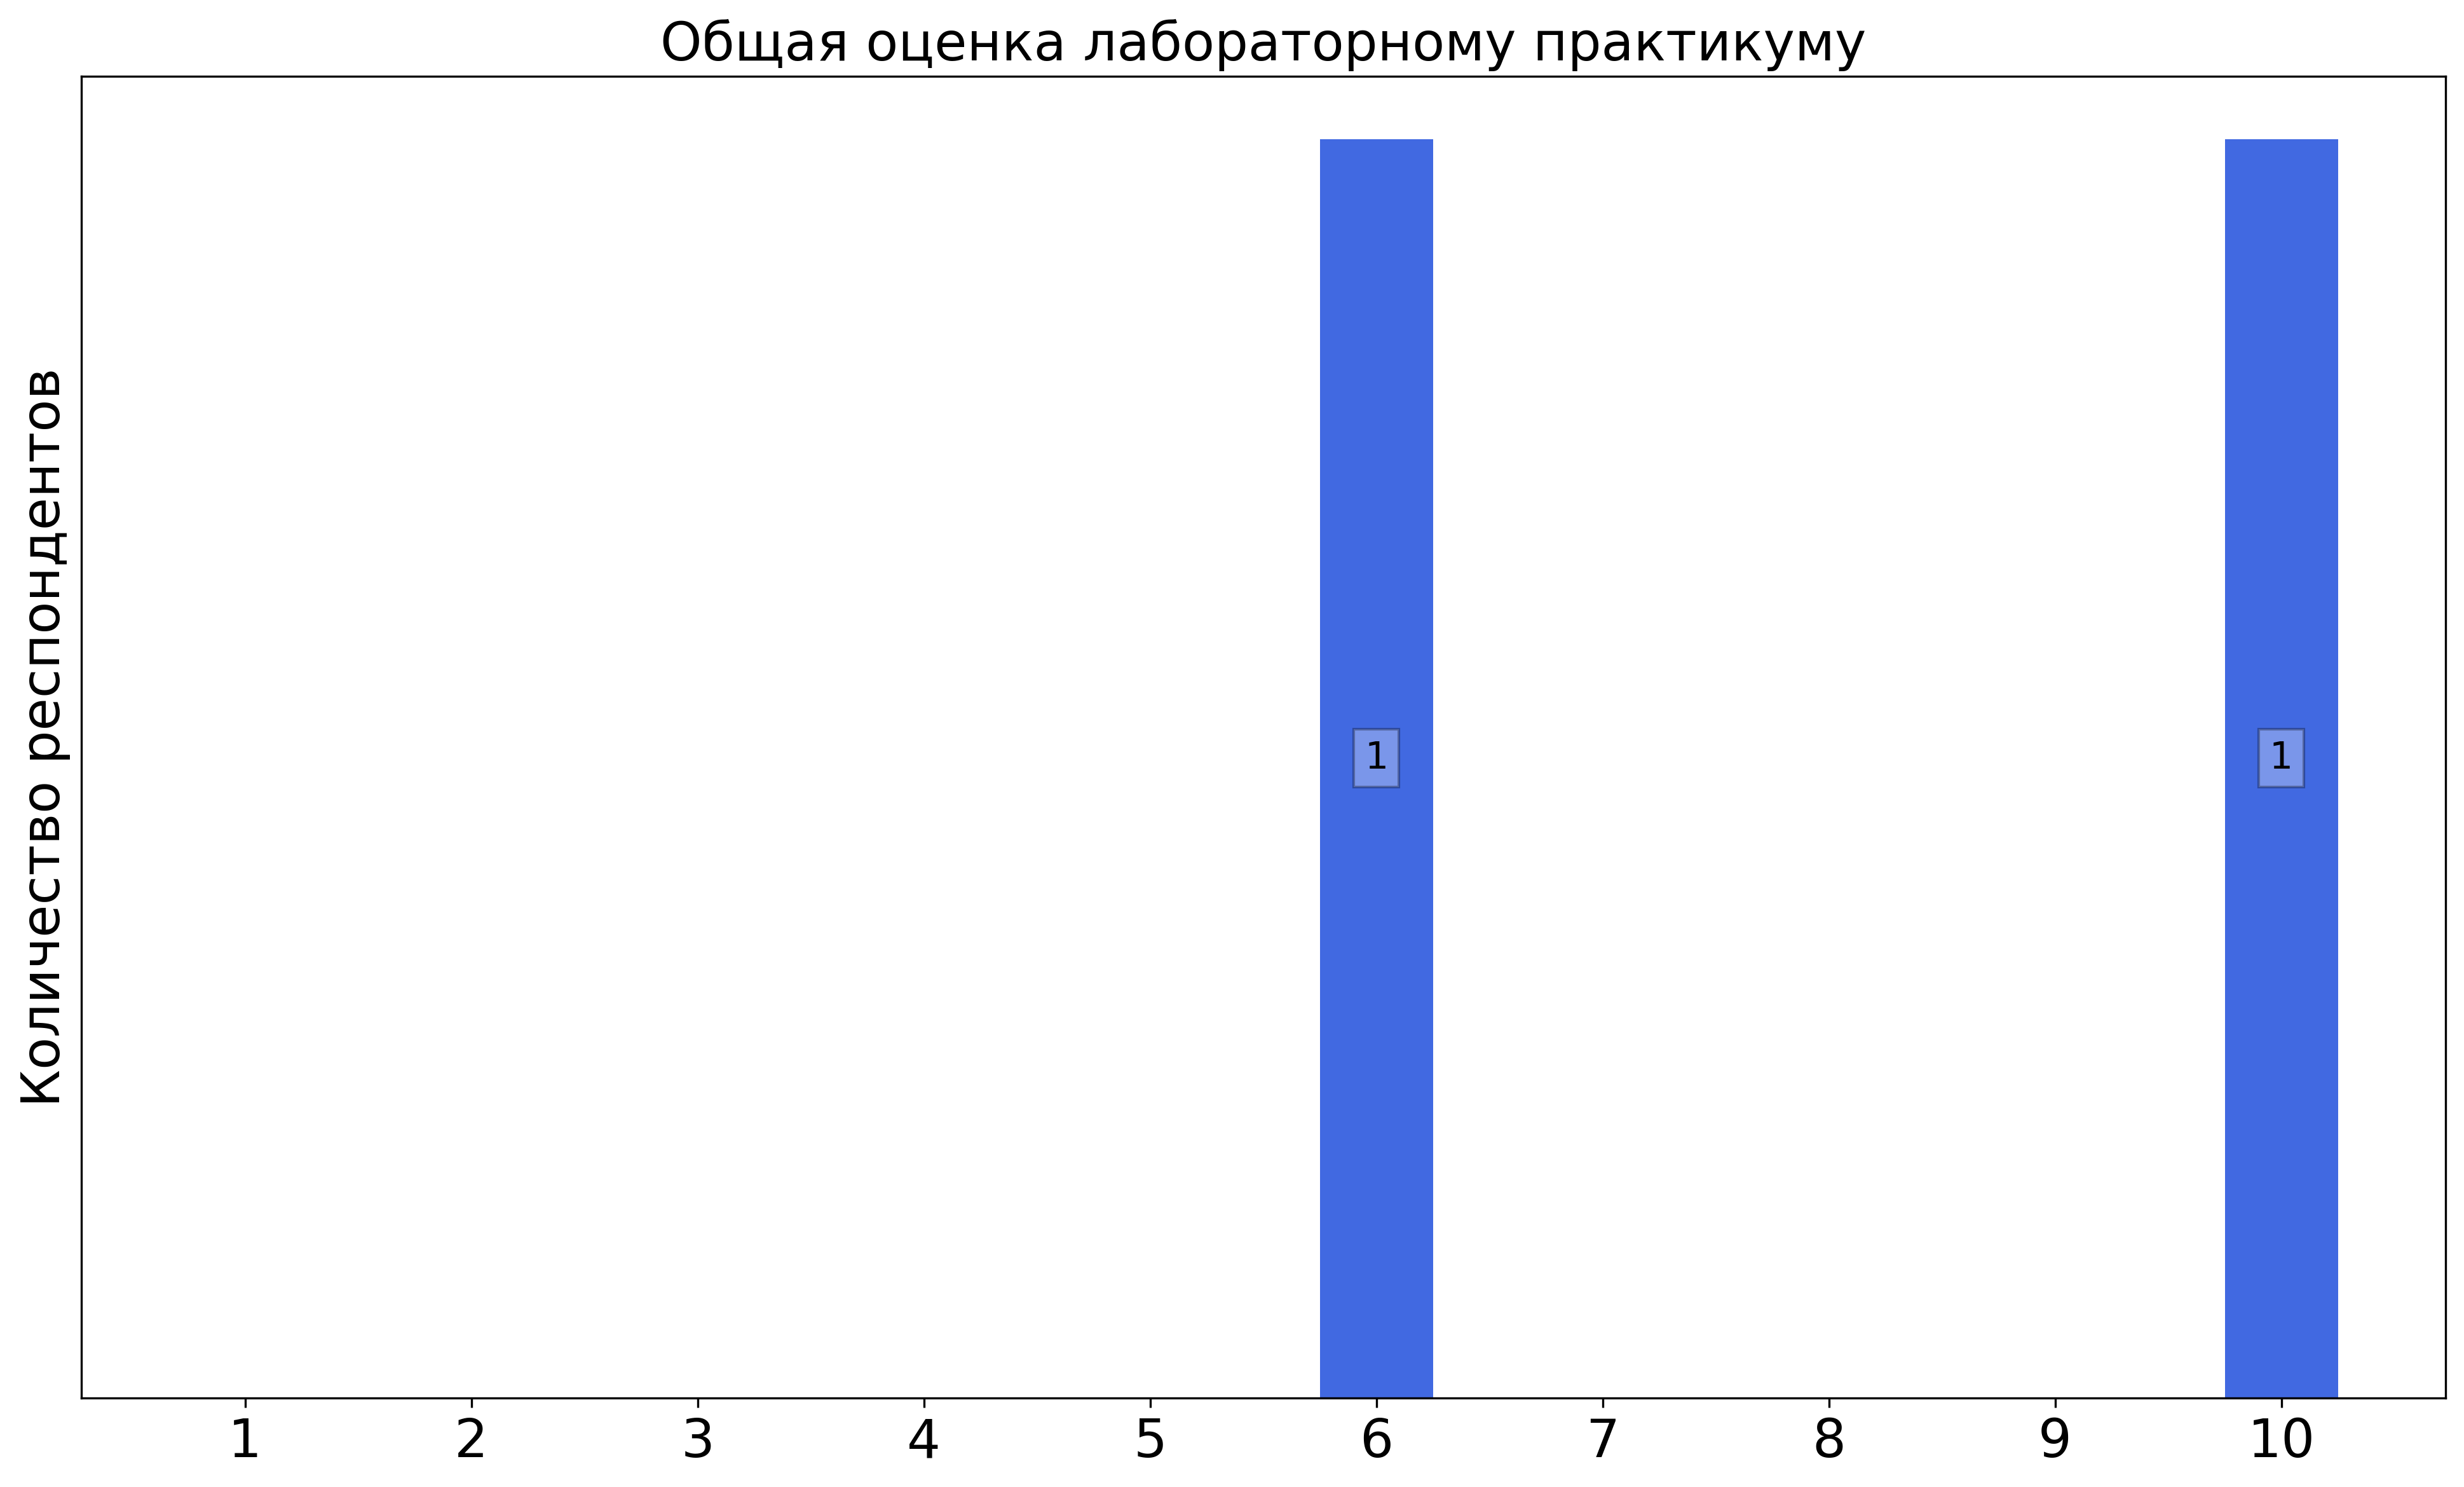
\includegraphics[width=\textwidth]{images/2 course/Радиотехнические цепи и сигналы/labniks-marks-Скурихин А.В.-3.png}
            \end{subfigure}	
            \caption{Оценки респондентов о качестве преподавания лабораторных работ}
        \end{figure}


    \subsubsection{Отзыв студентов о лабораторных работах. Преподаватель: Суханов А.А.}
        \begin{figure}[H]
            \centering
            \begin{subfigure}[b]{0.45\textwidth}
                \centering
                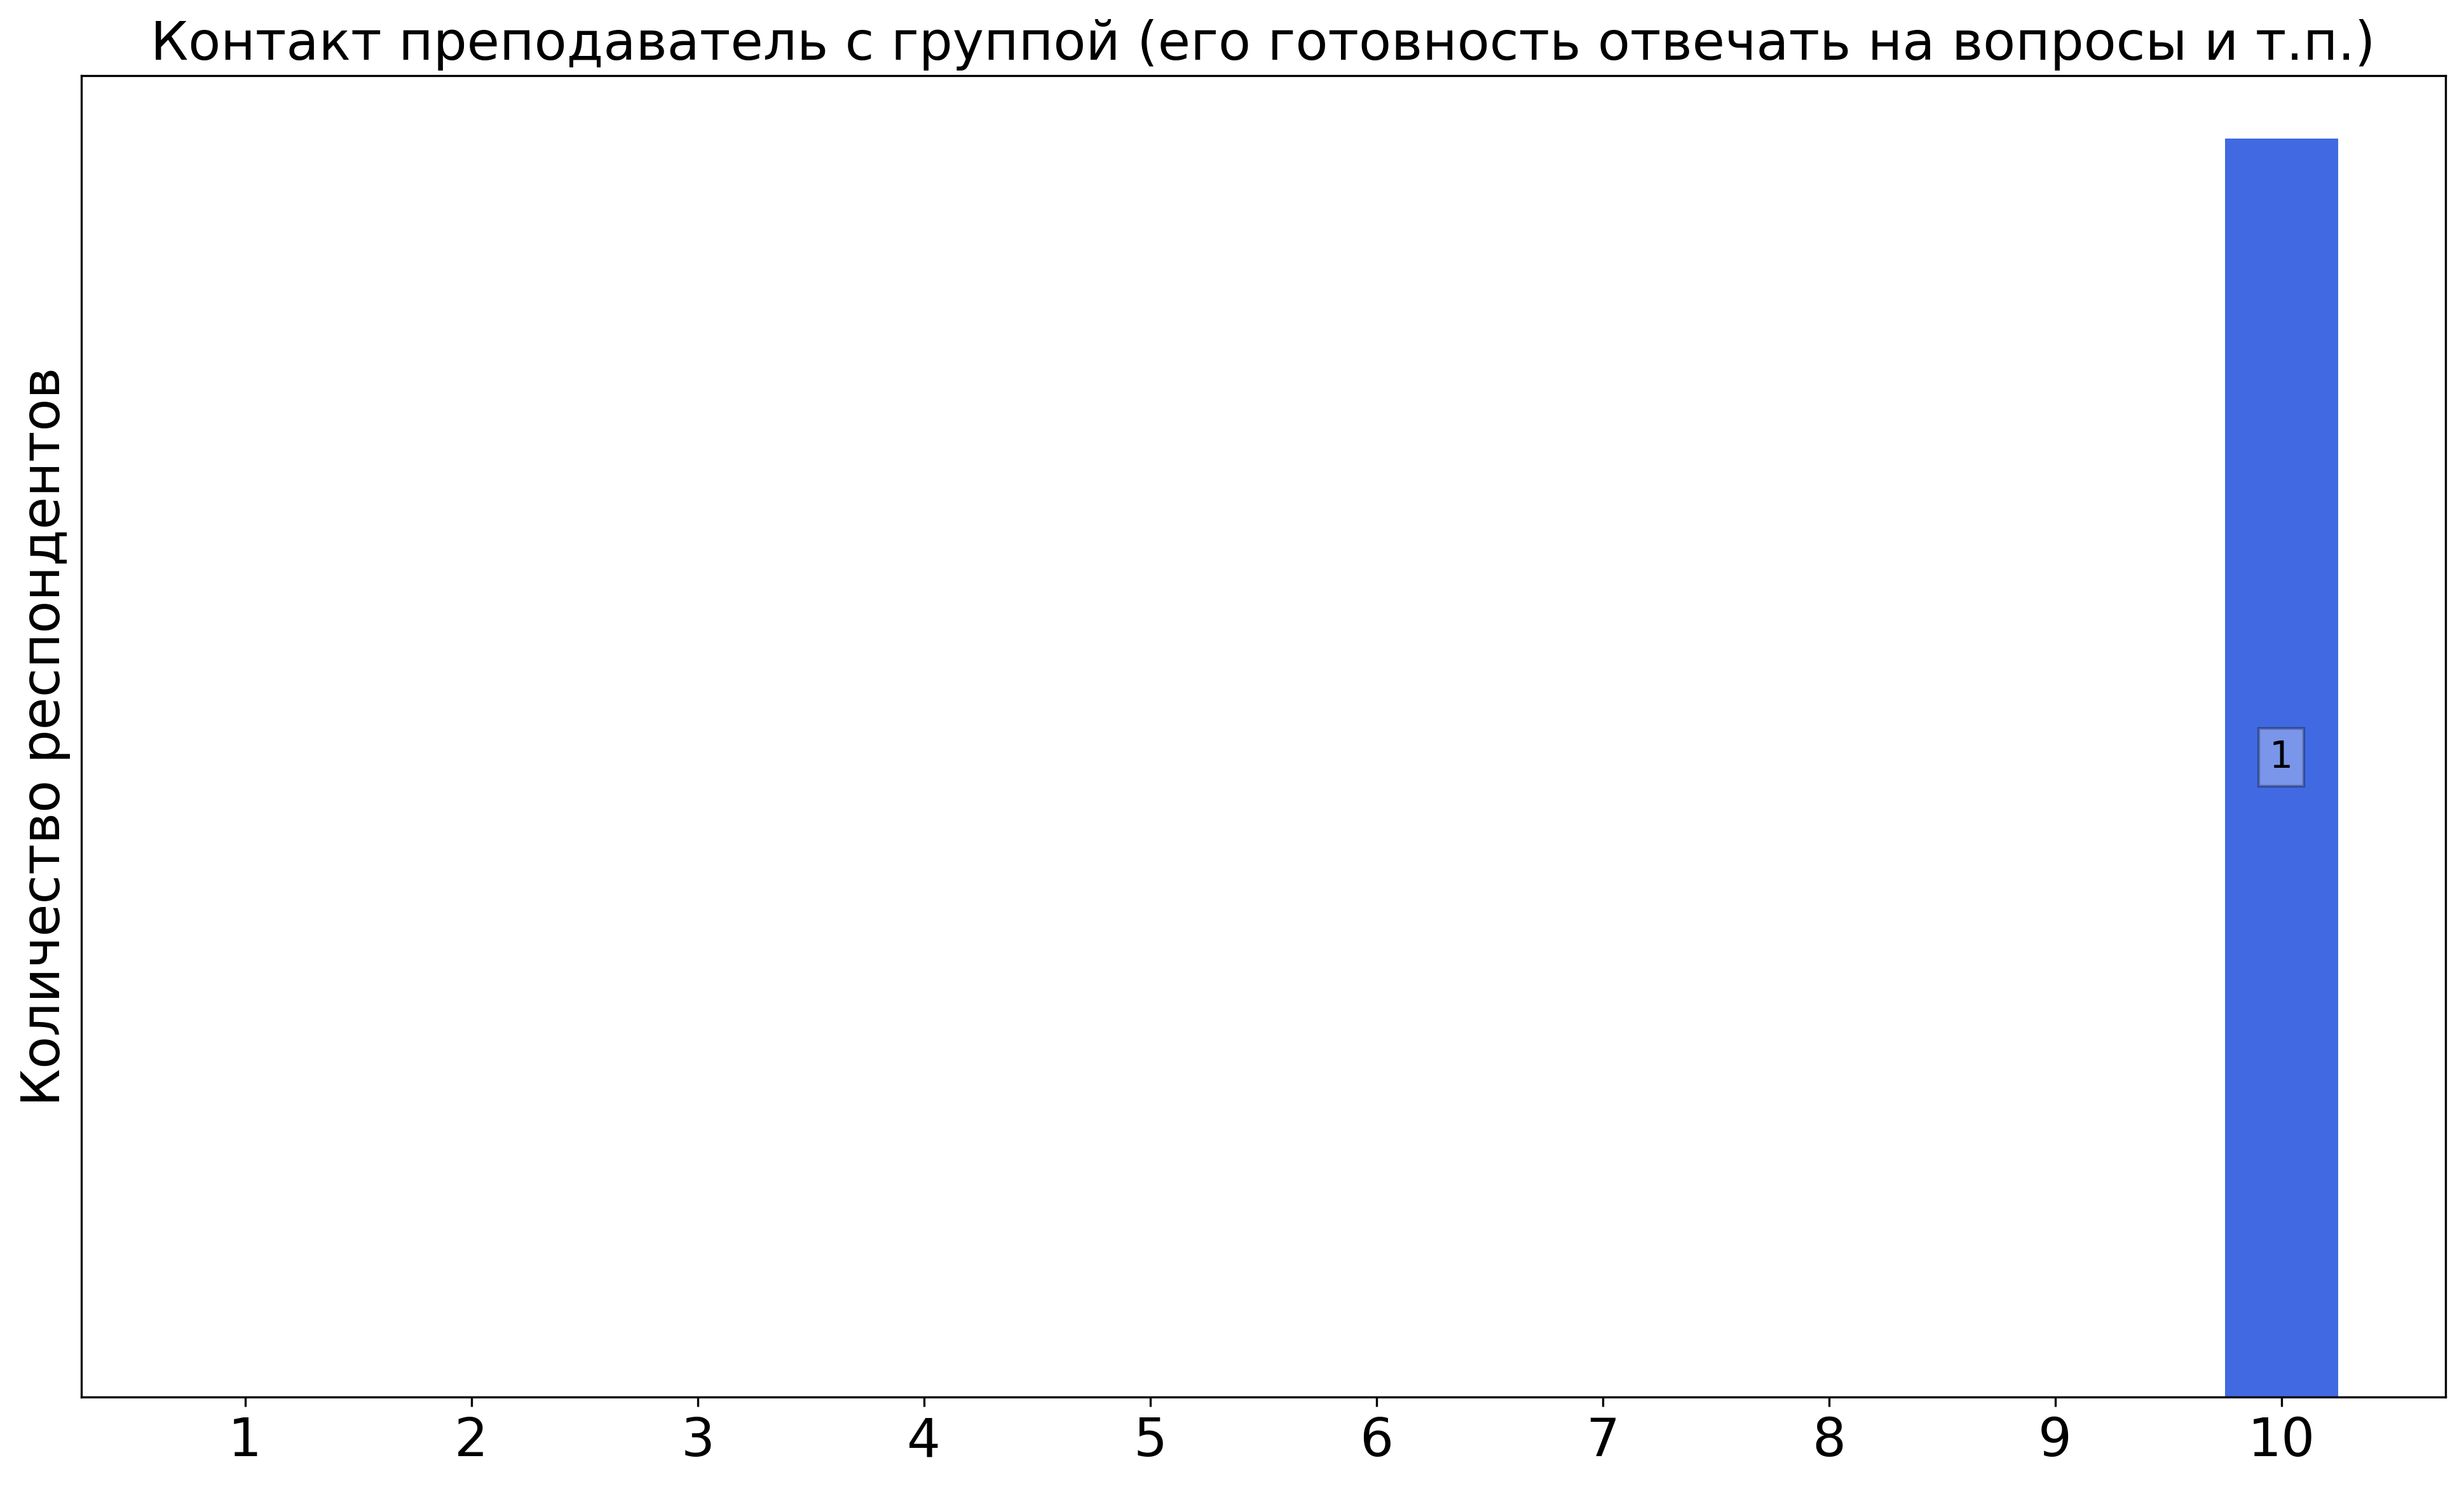
\includegraphics[width=\textwidth]{images/2 course/Радиотехнические цепи и сигналы/labniks-marks-Суханов А.А.-0.png}
            \end{subfigure}
            \begin{subfigure}[b]{0.45\textwidth}
                \centering
                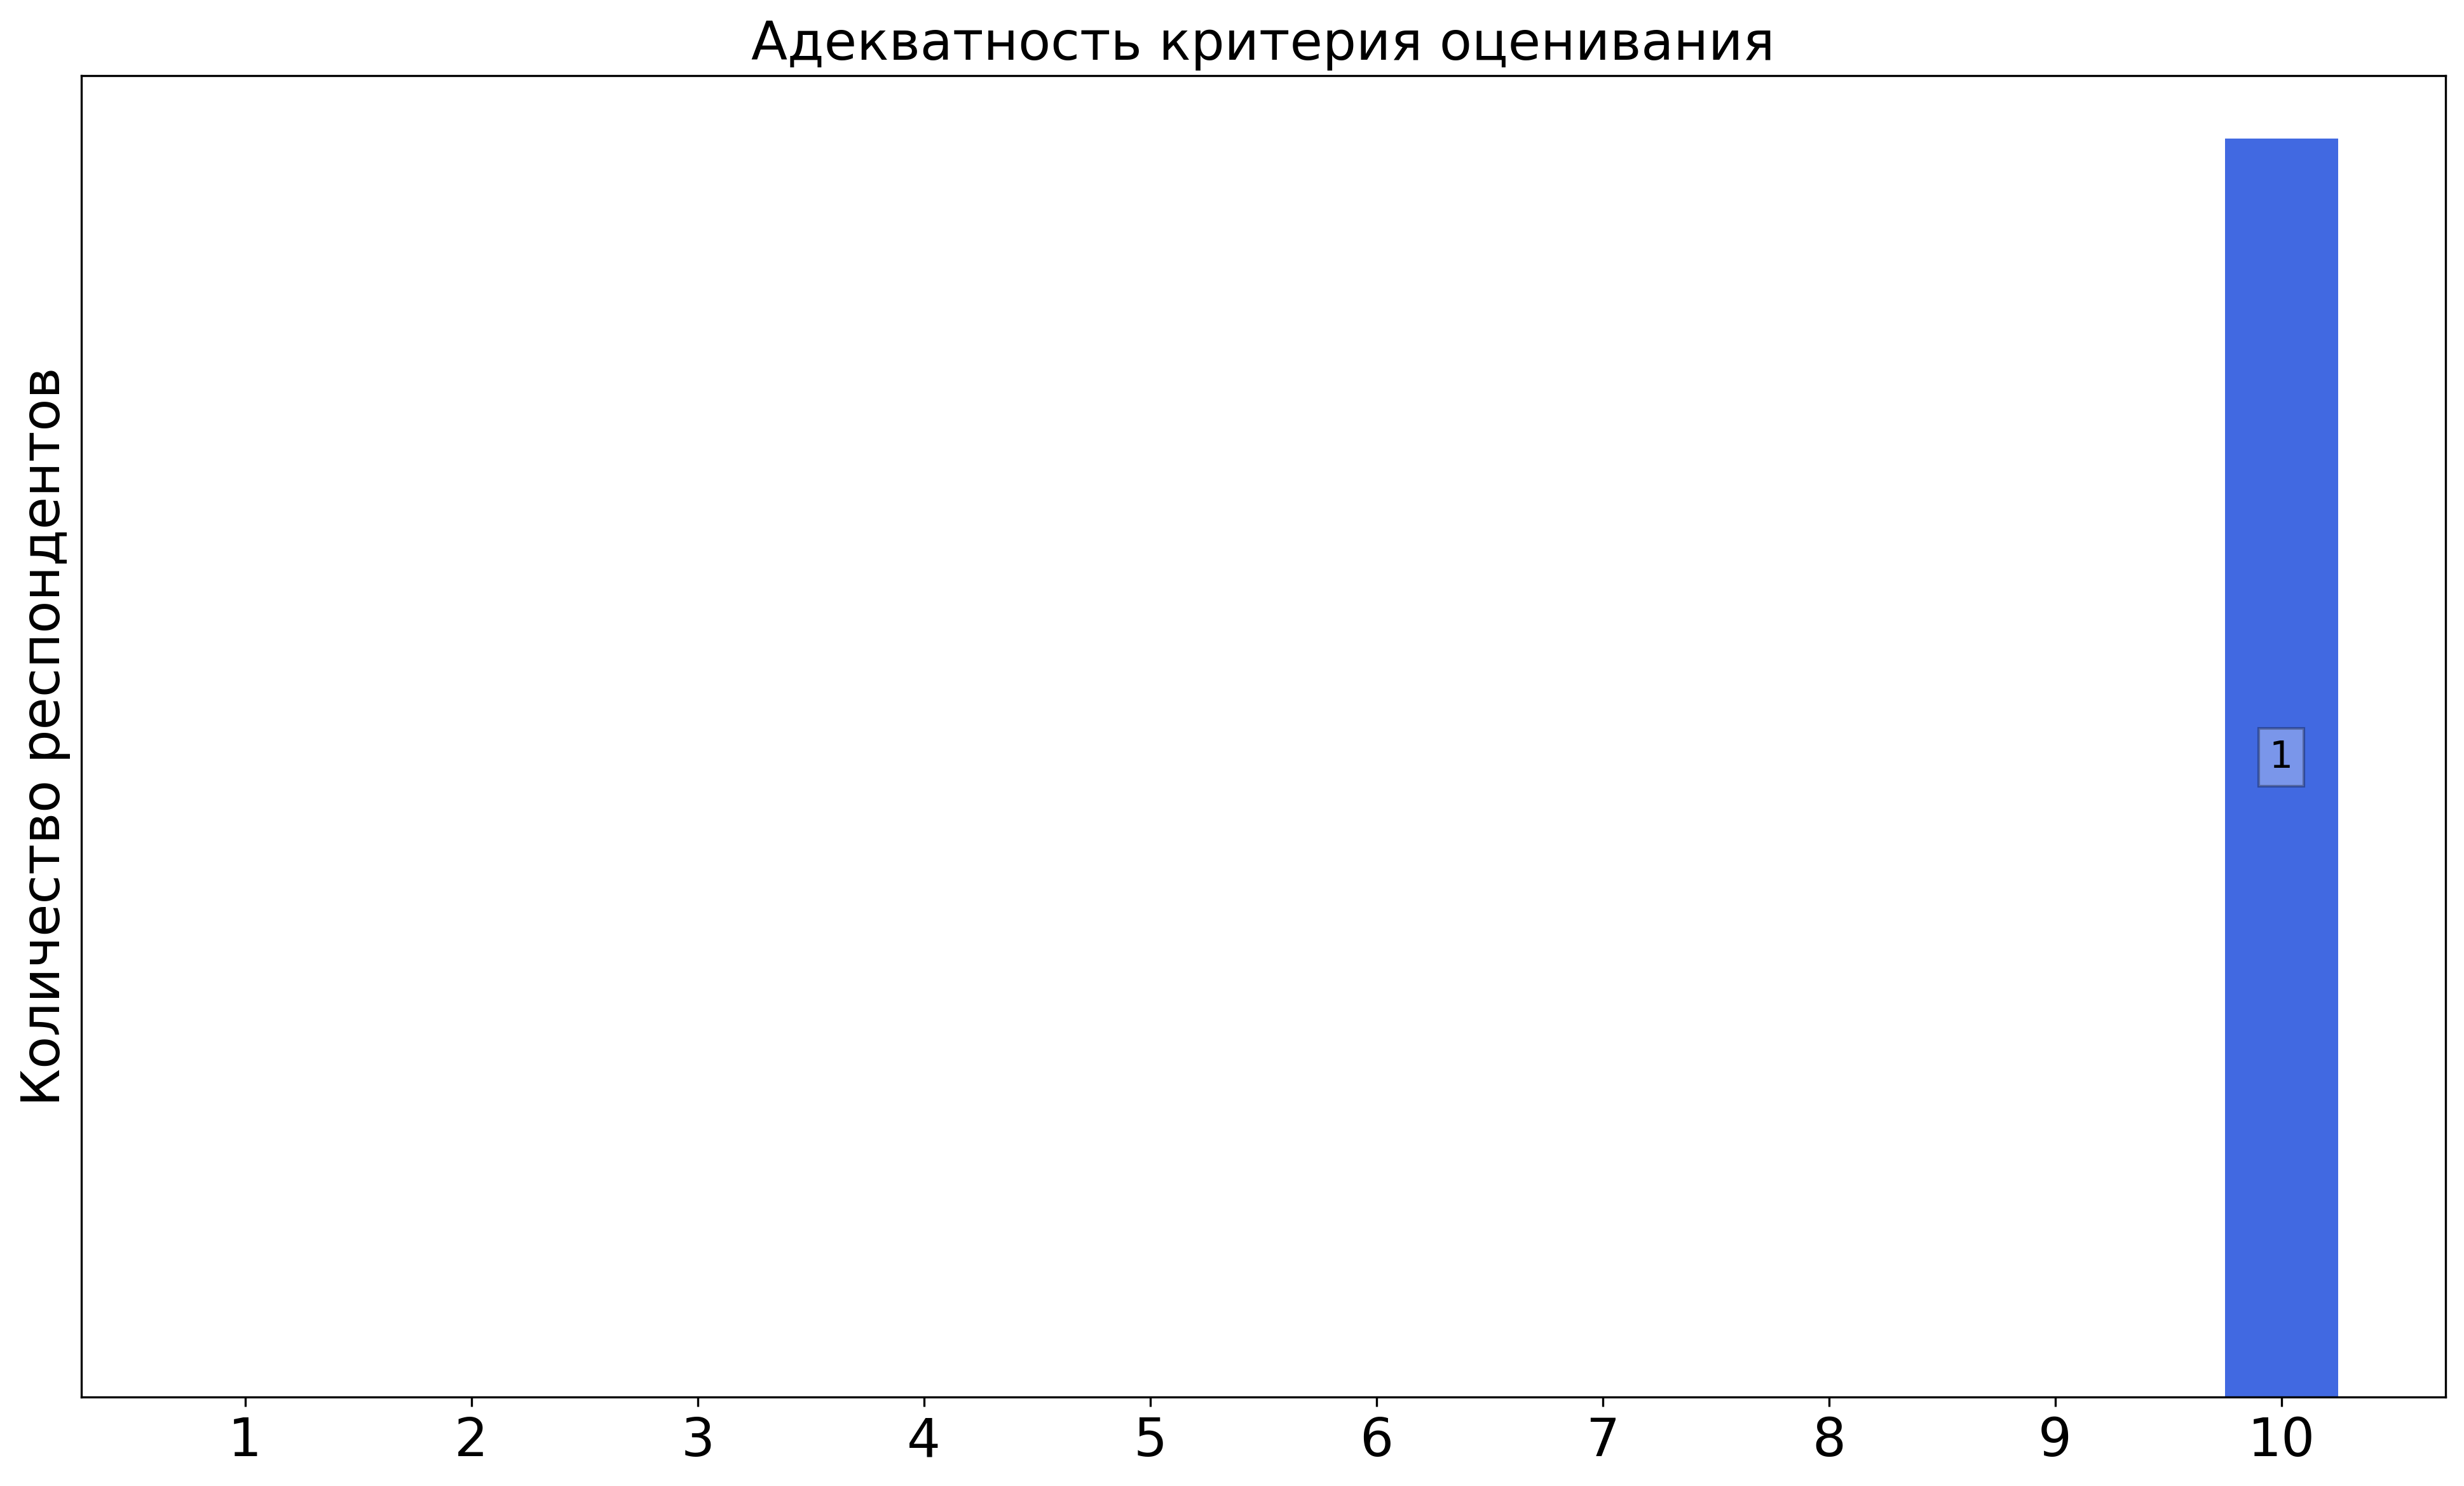
\includegraphics[width=\textwidth]{images/2 course/Радиотехнические цепи и сигналы/labniks-marks-Суханов А.А.-1.png}
            \end{subfigure}
            \begin{subfigure}[b]{0.45\textwidth}
                \centering
                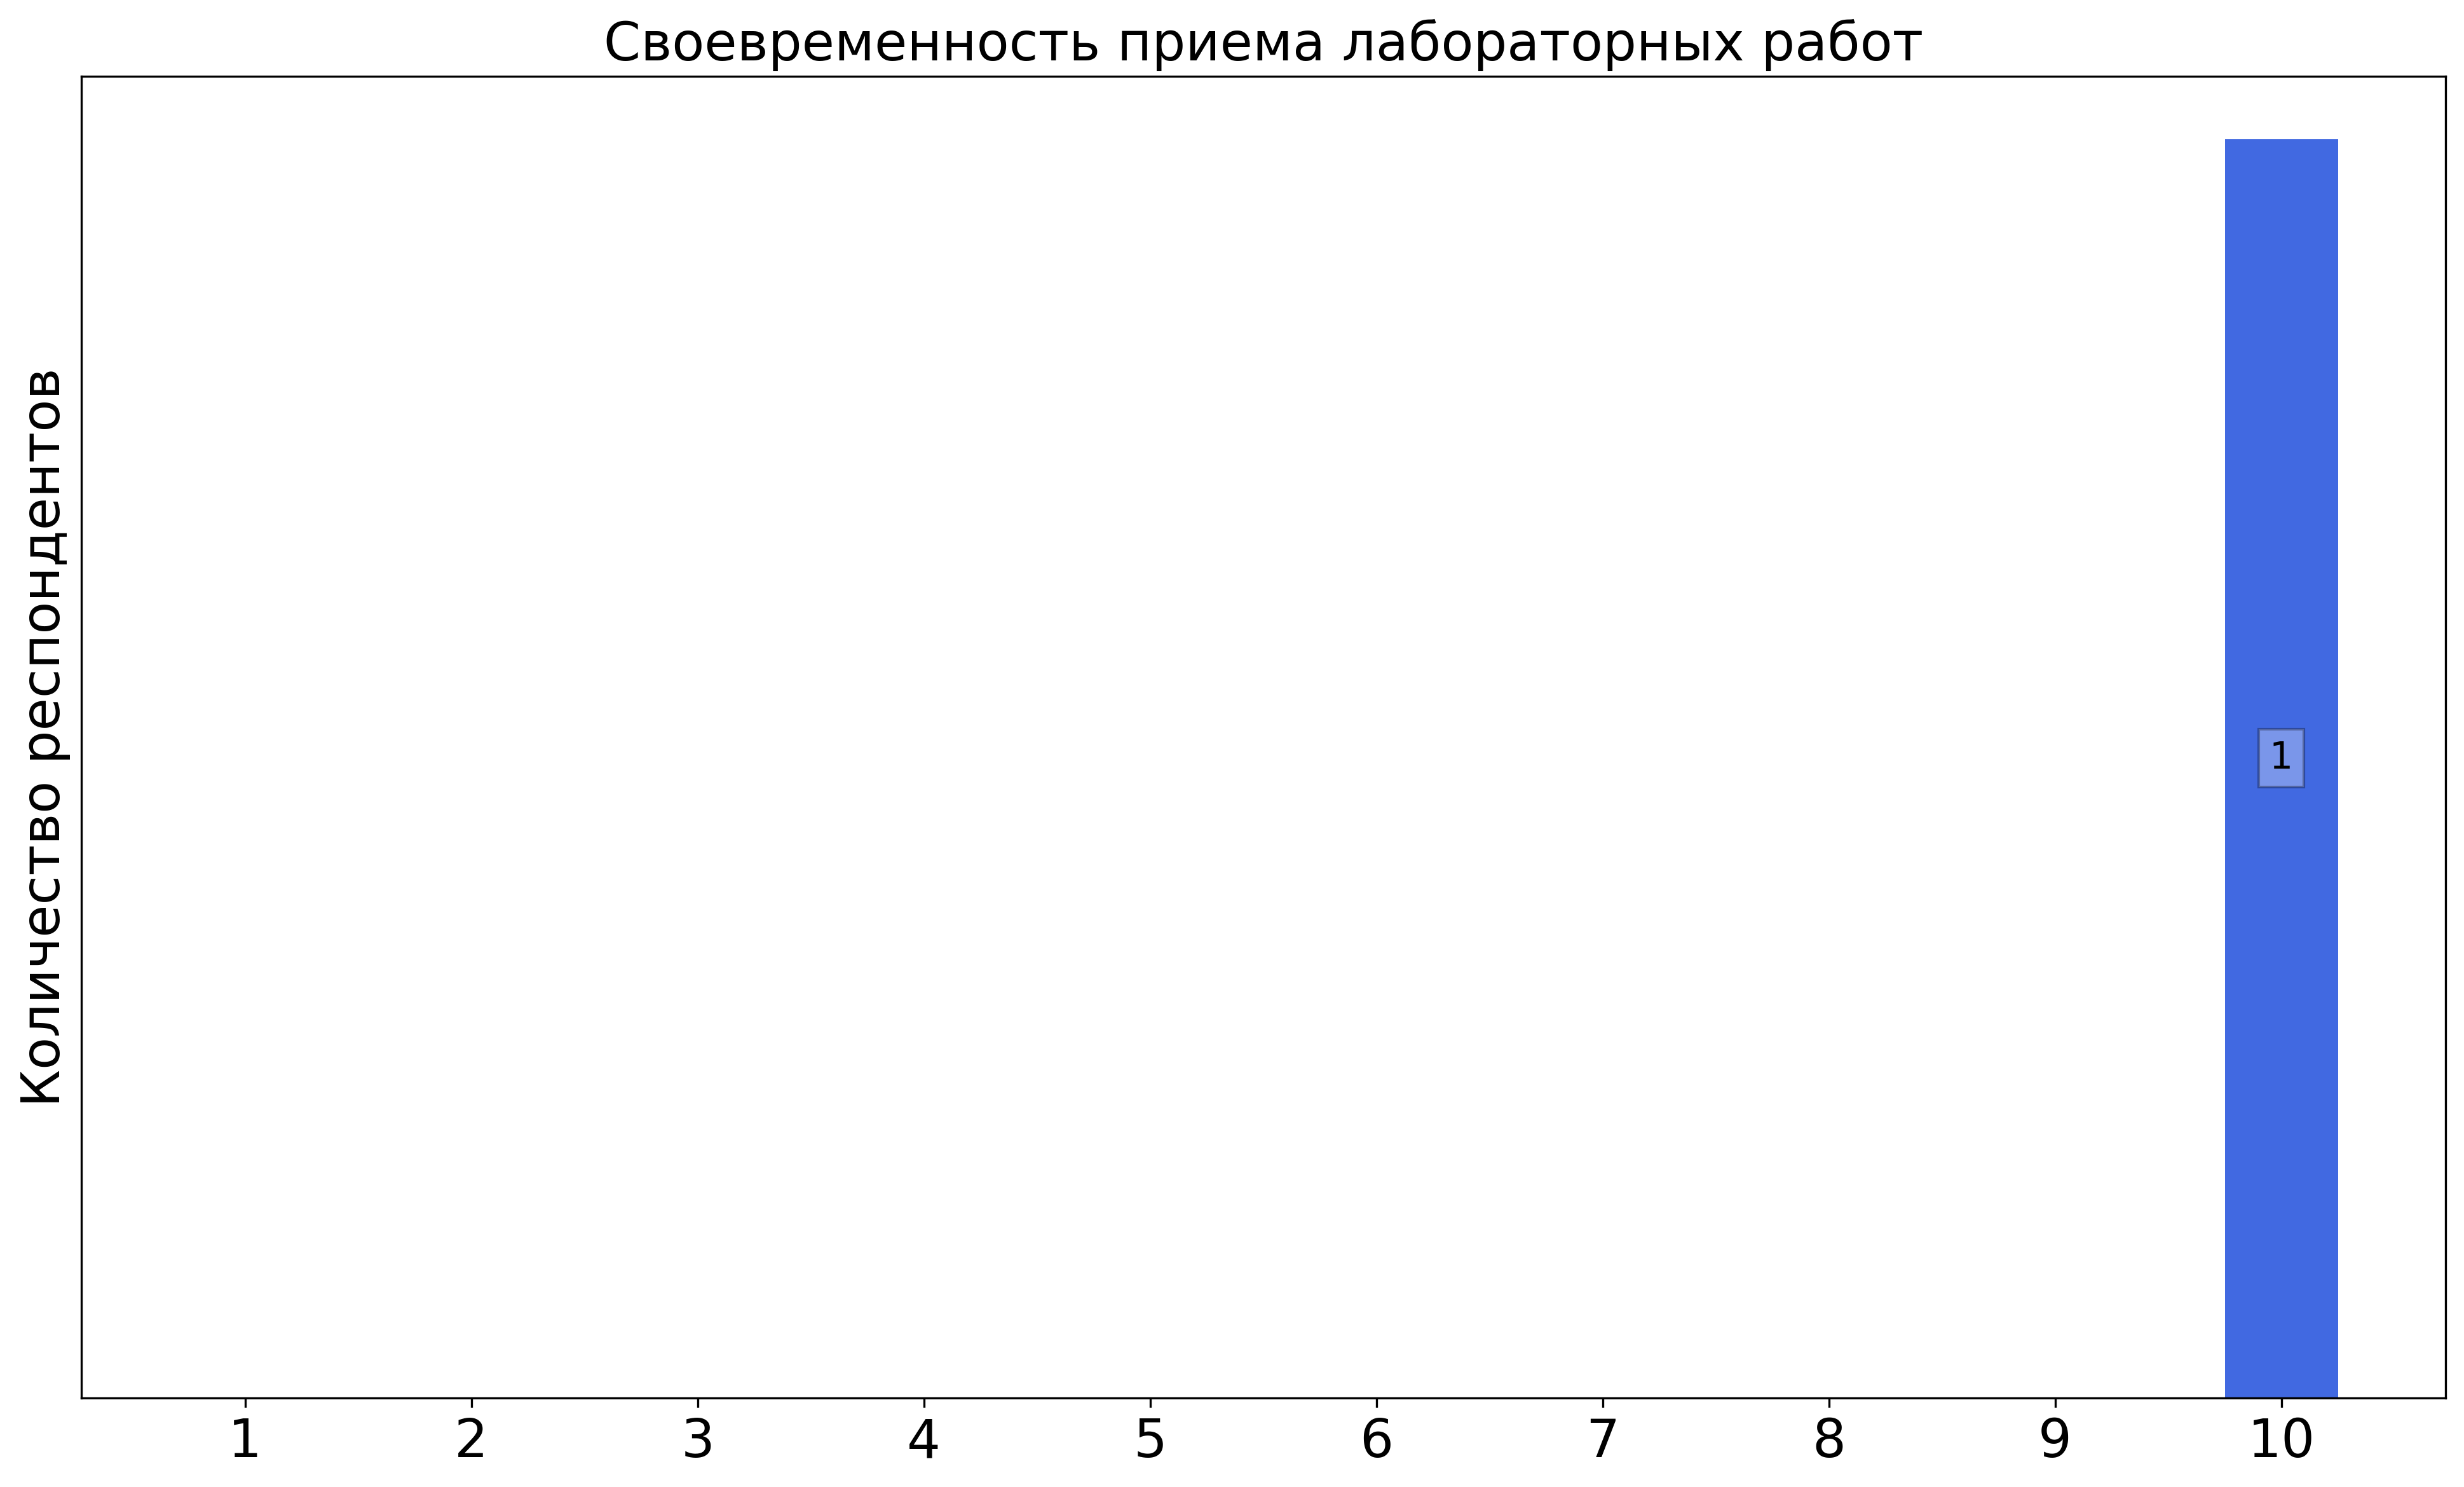
\includegraphics[width=\textwidth]{images/2 course/Радиотехнические цепи и сигналы/labniks-marks-Суханов А.А.-2.png}
            \end{subfigure}
            \begin{subfigure}[b]{0.45\textwidth}
                \centering
                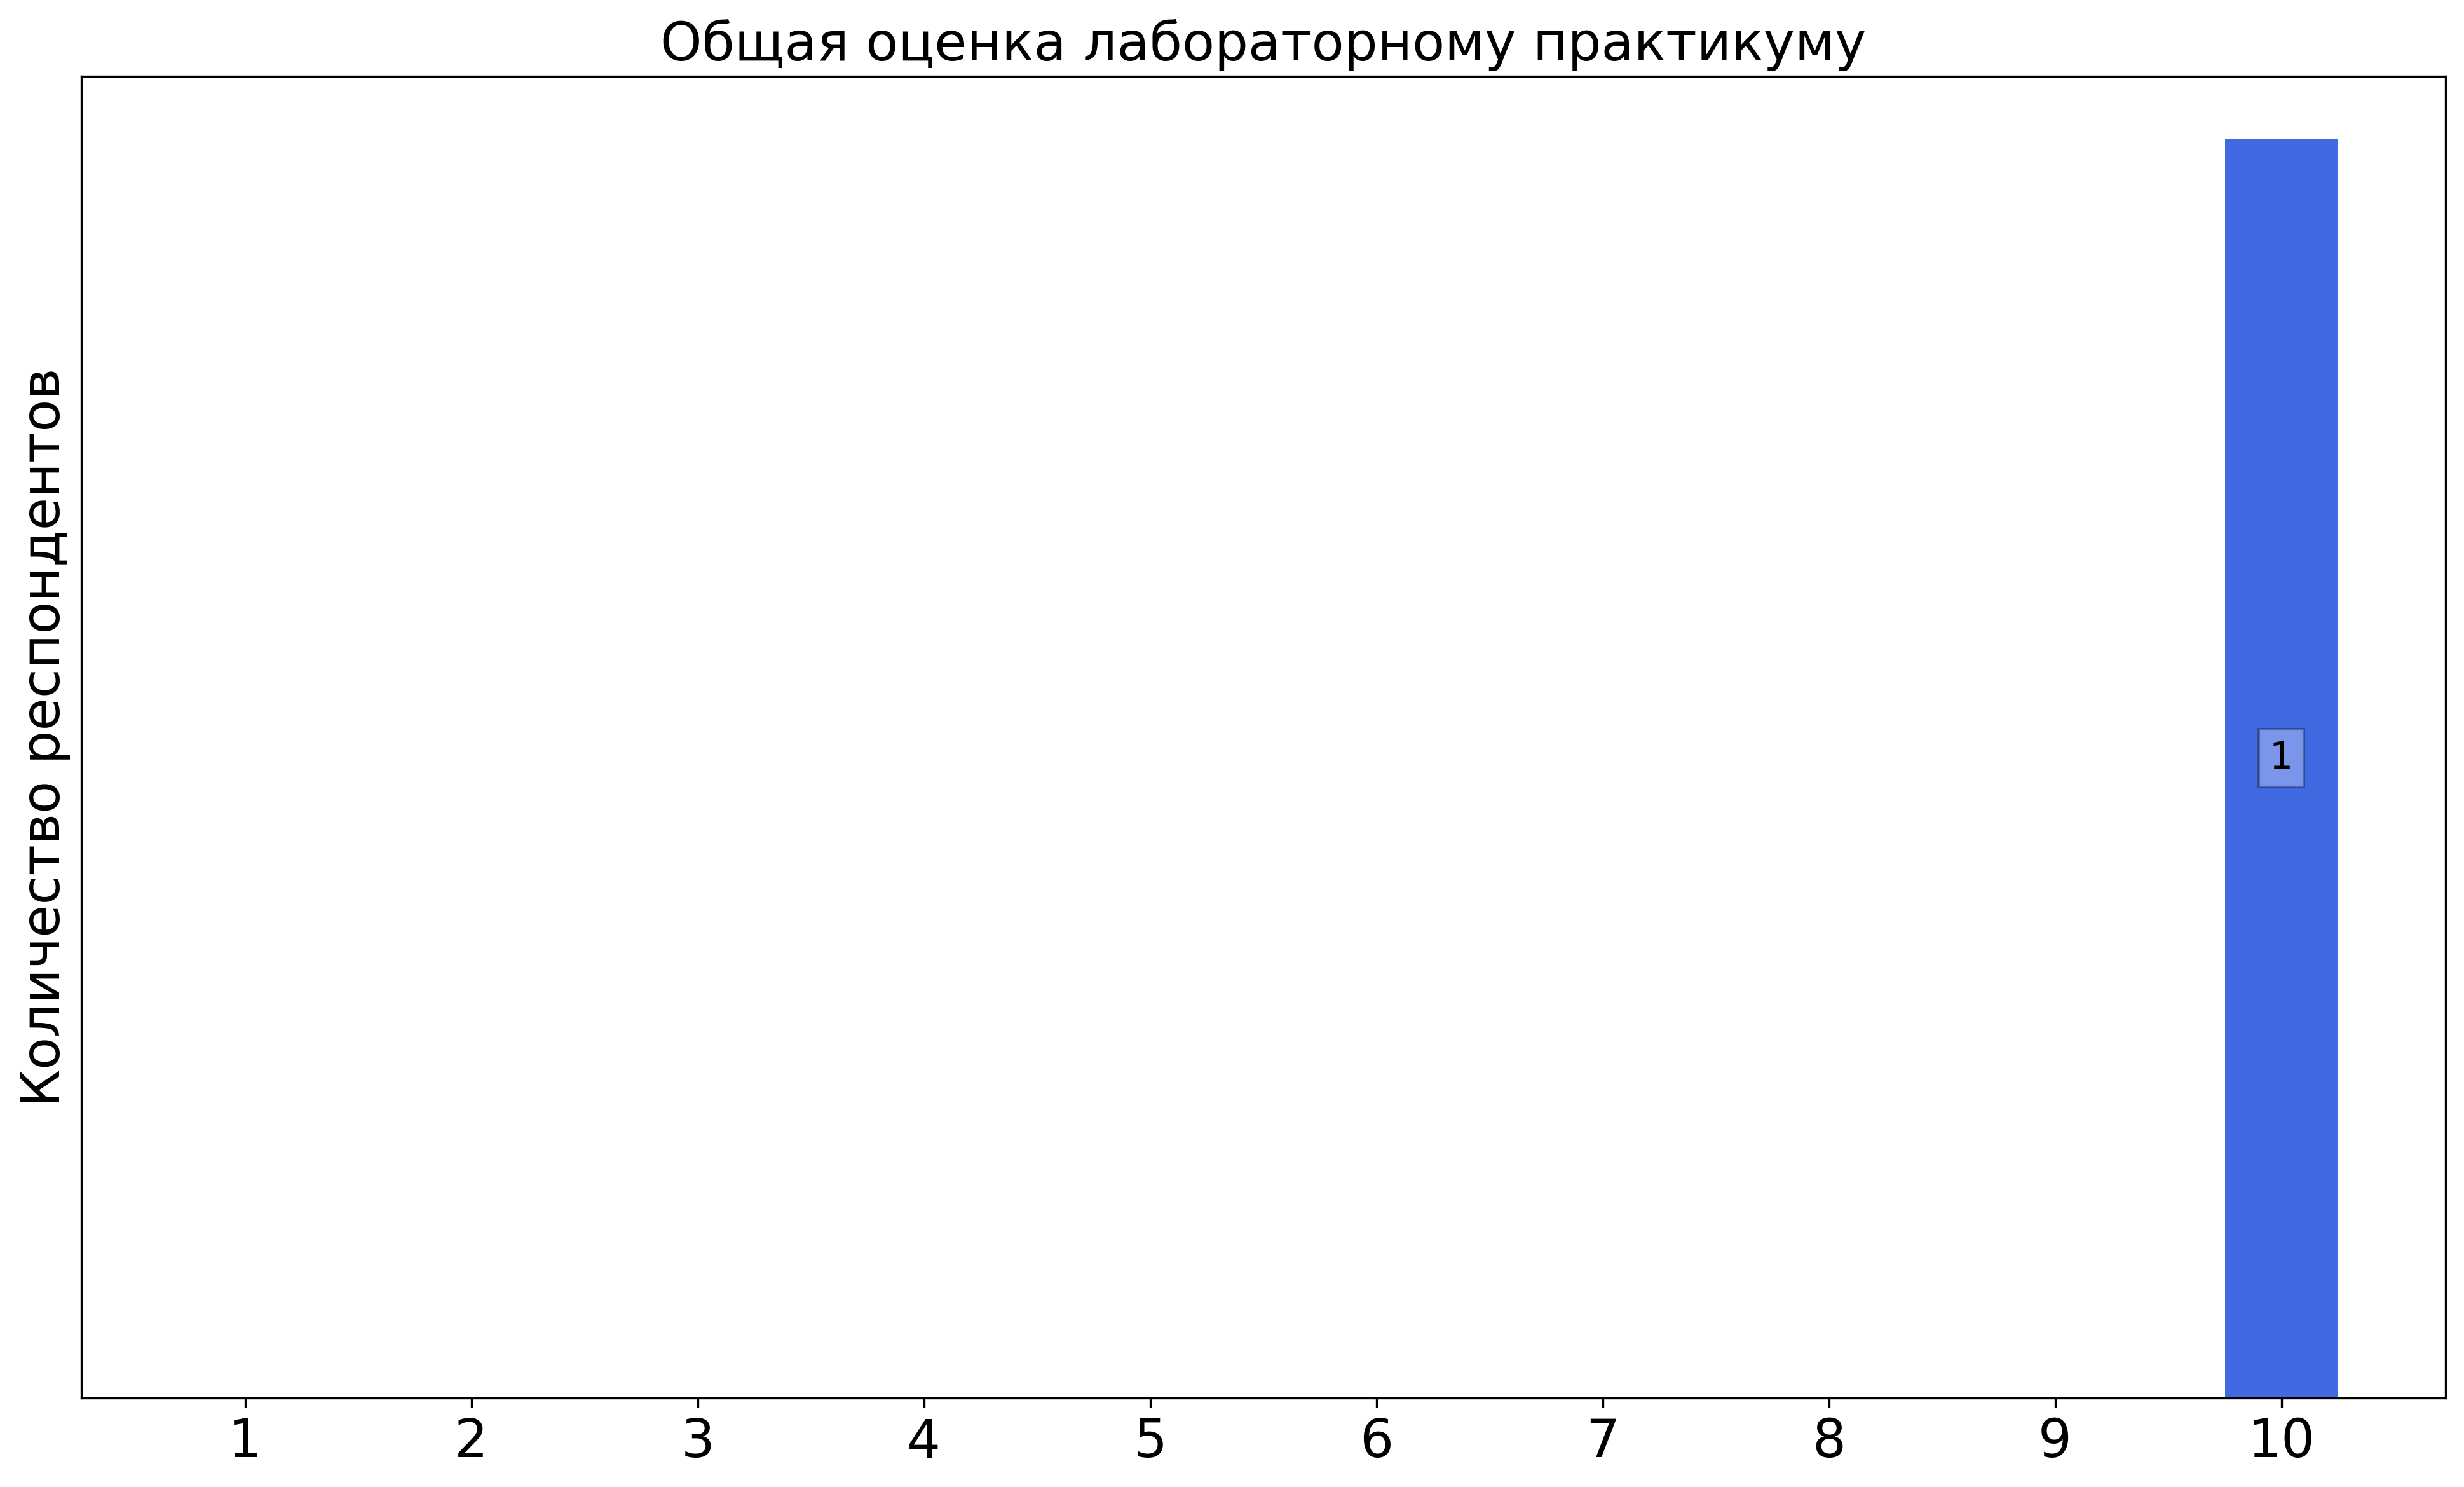
\includegraphics[width=\textwidth]{images/2 course/Радиотехнические цепи и сигналы/labniks-marks-Суханов А.А.-3.png}
            \end{subfigure}	
            \caption{Оценки респондентов о качестве преподавания лабораторных работ}
        \end{figure}


        
    \subsubsection{Отзыв студентов о лабораторных работах. Преподаватель: Филатов И.В.}
        \begin{figure}[H]
            \centering
            \begin{subfigure}[b]{0.45\textwidth}
                \centering
                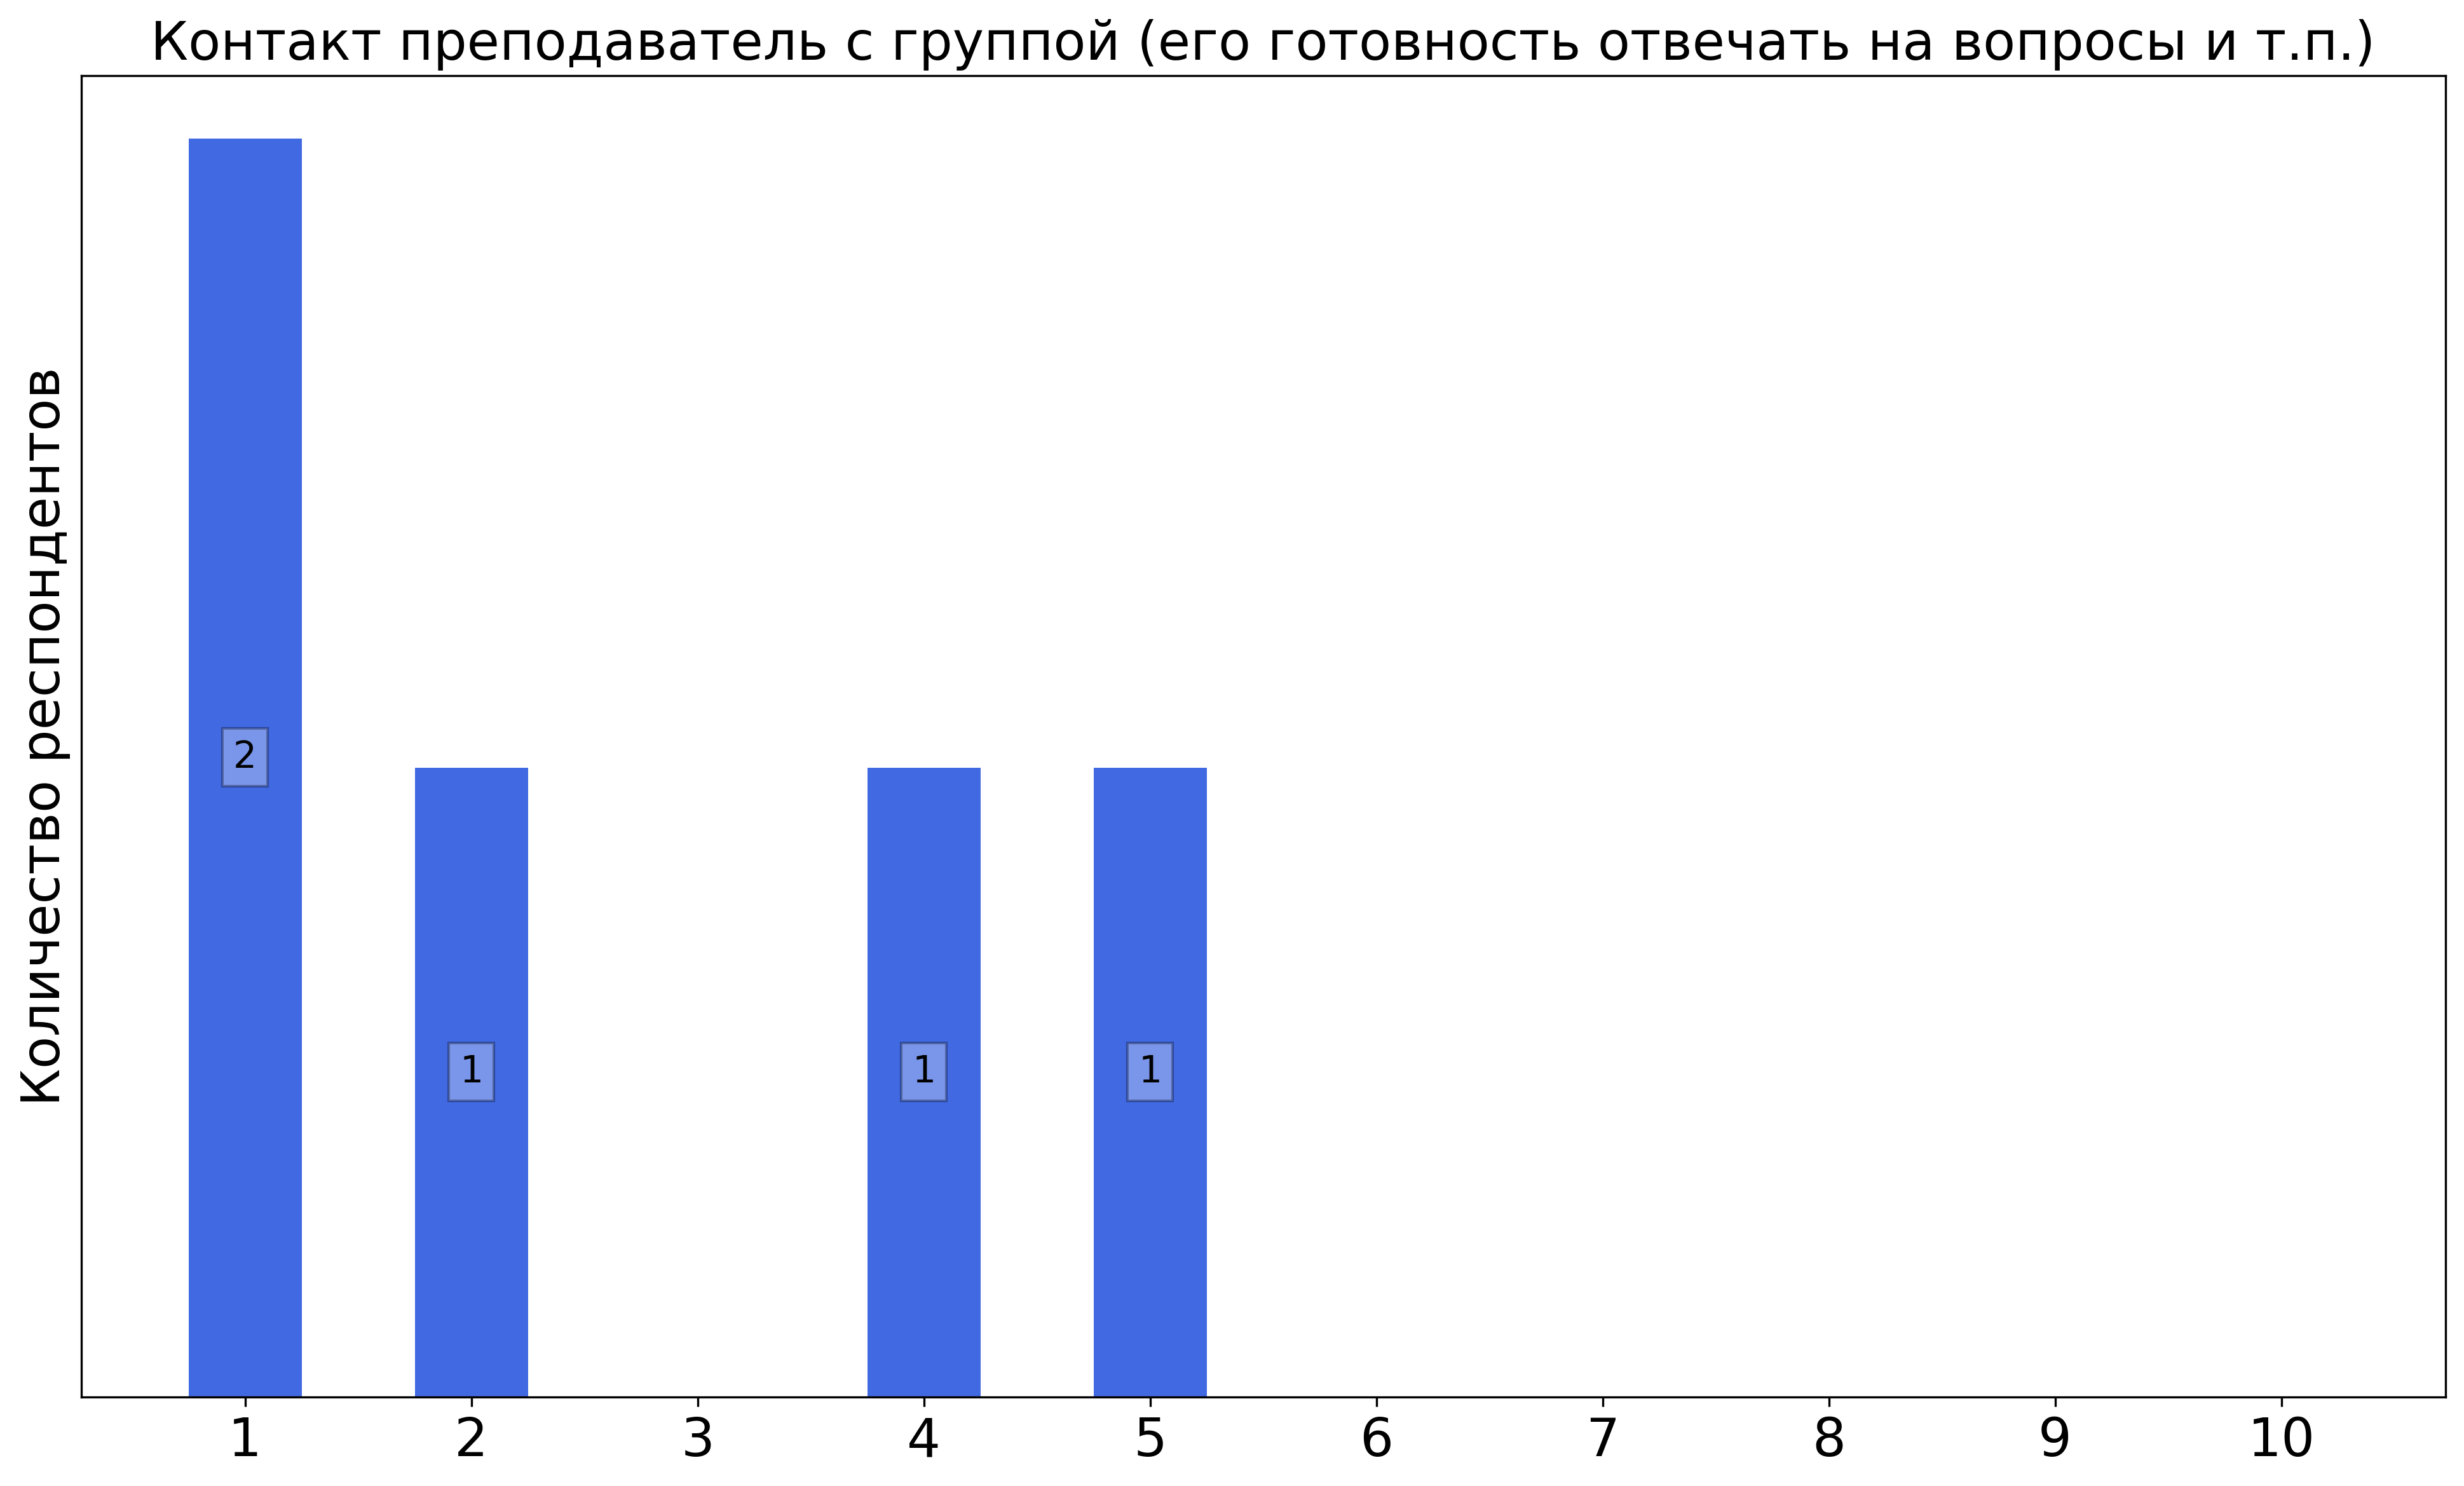
\includegraphics[width=\textwidth]{images/2 course/Радиотехнические цепи и сигналы/labniks-marks-Филатов И.В.-0.png}
            \end{subfigure}
            \begin{subfigure}[b]{0.45\textwidth}
                \centering
                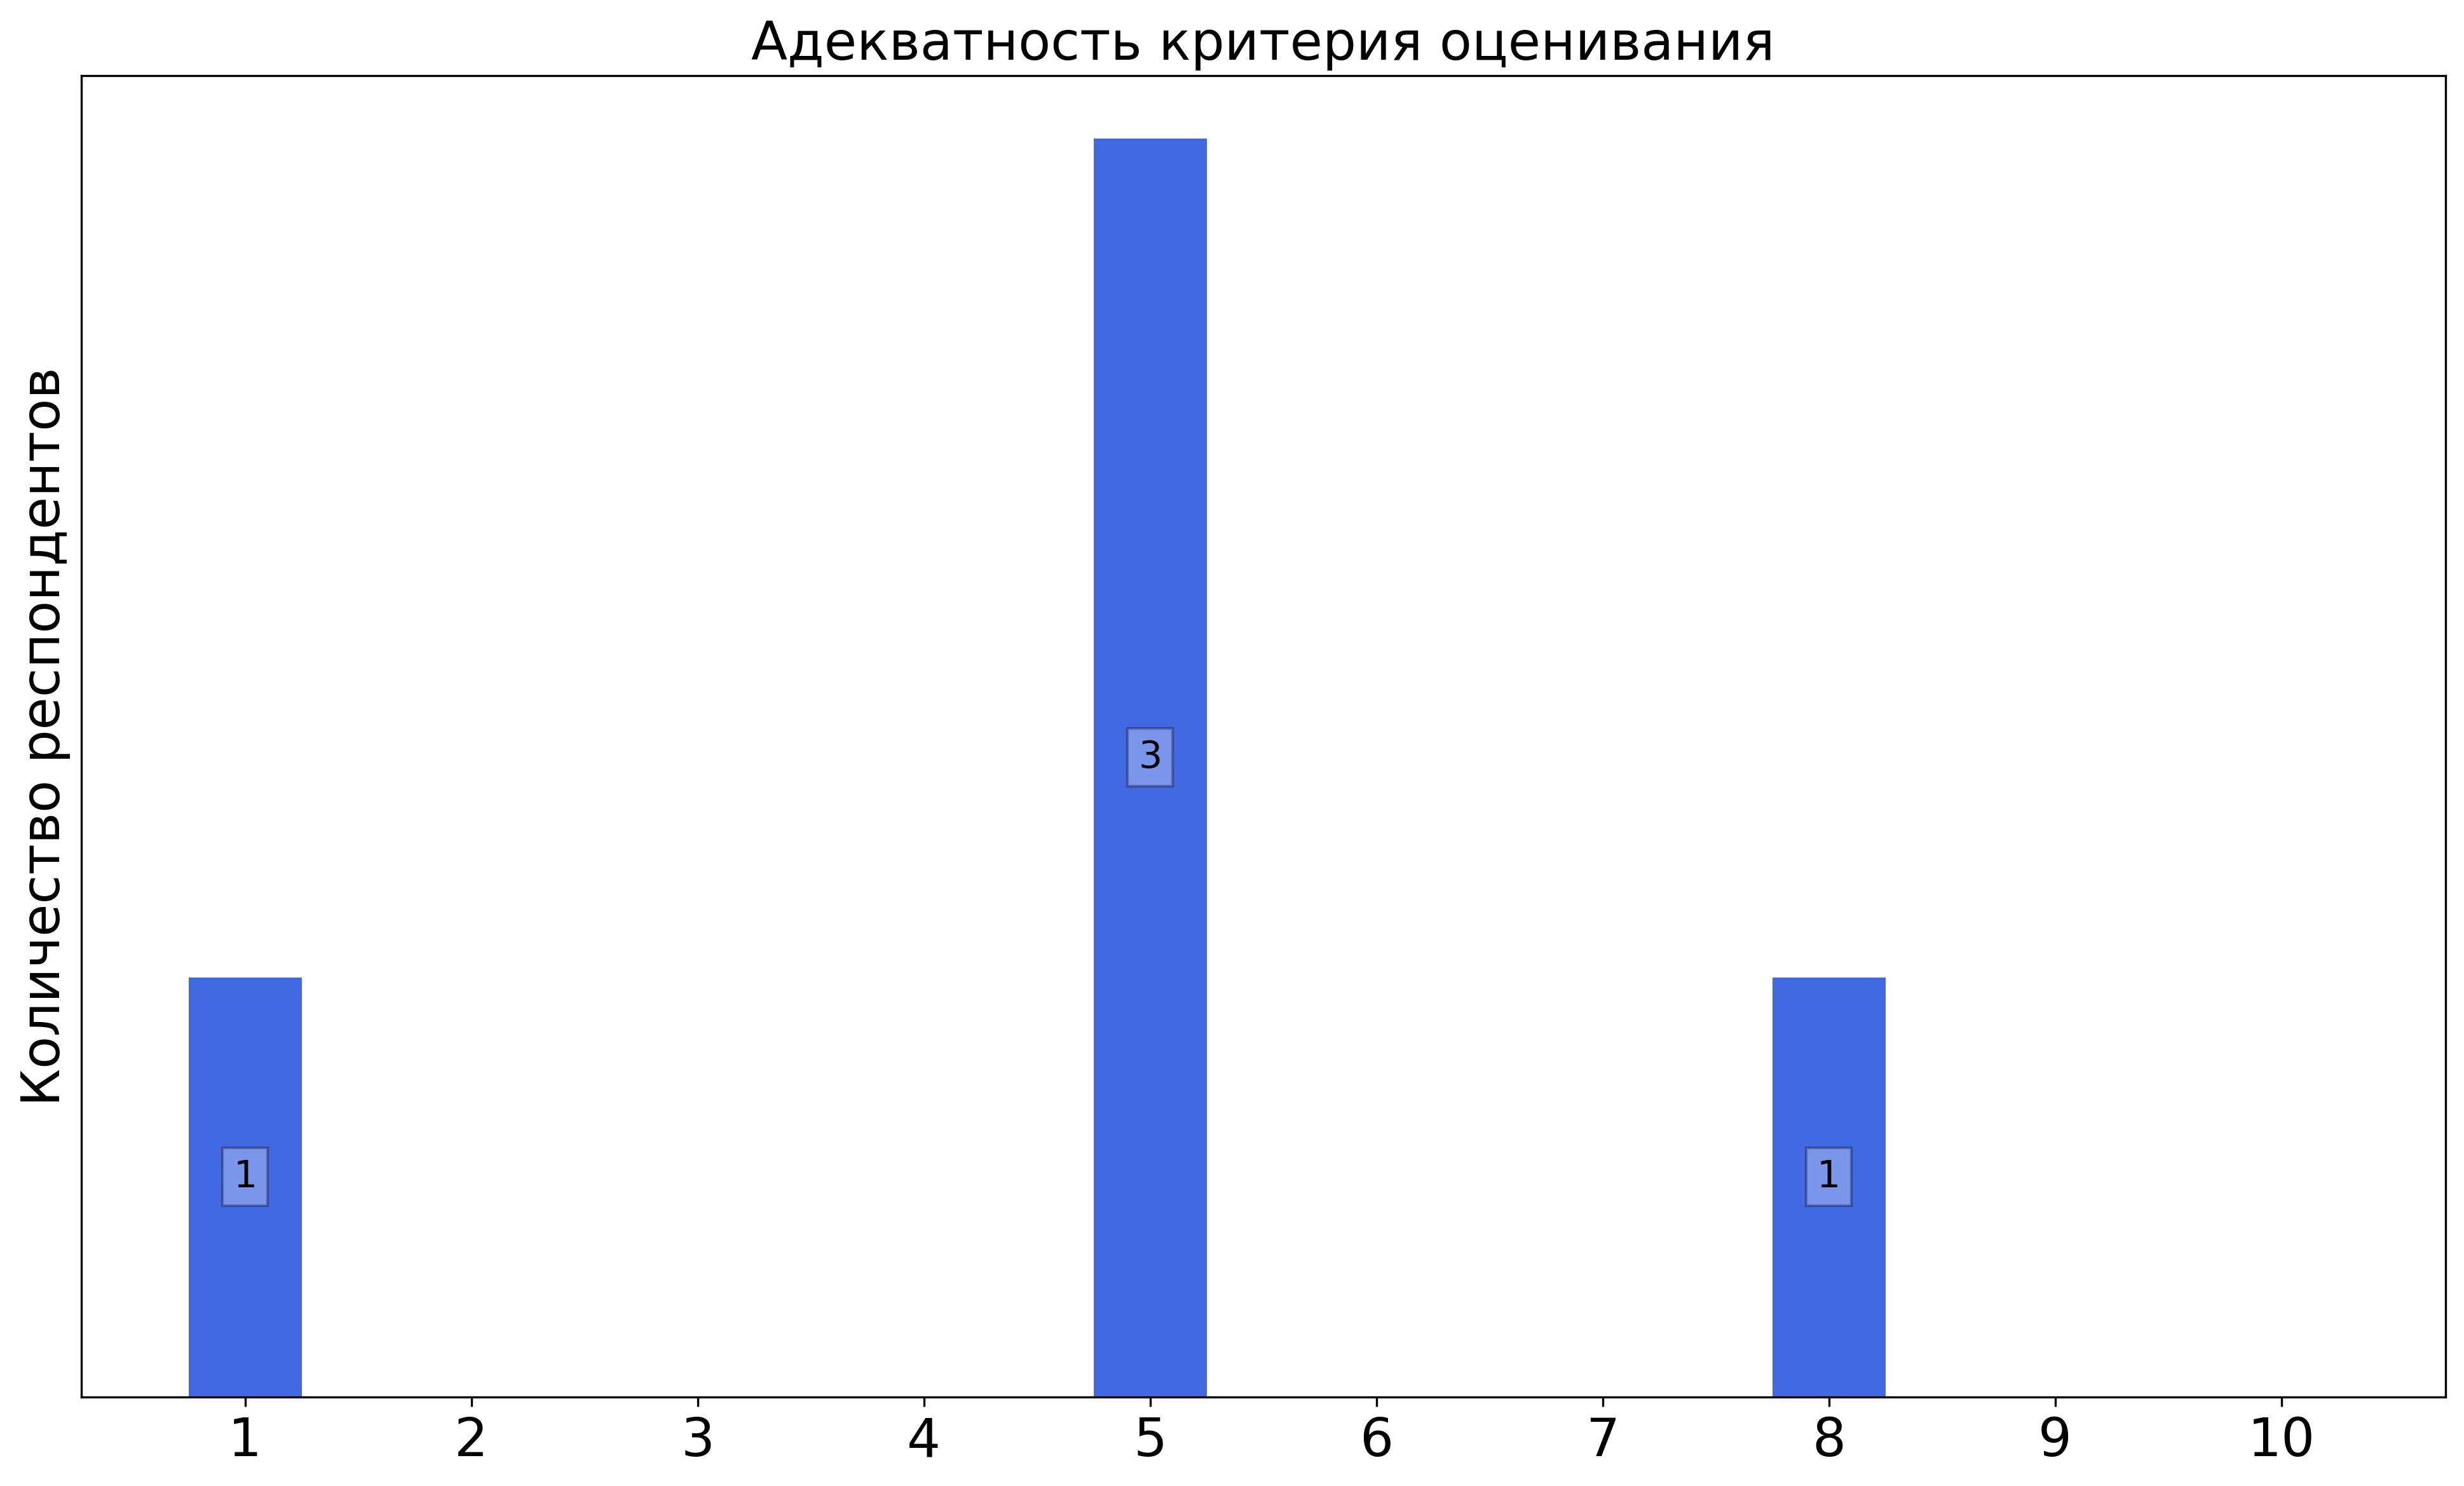
\includegraphics[width=\textwidth]{images/2 course/Радиотехнические цепи и сигналы/labniks-marks-Филатов И.В.-1.png}
            \end{subfigure}
            \begin{subfigure}[b]{0.45\textwidth}
                \centering
                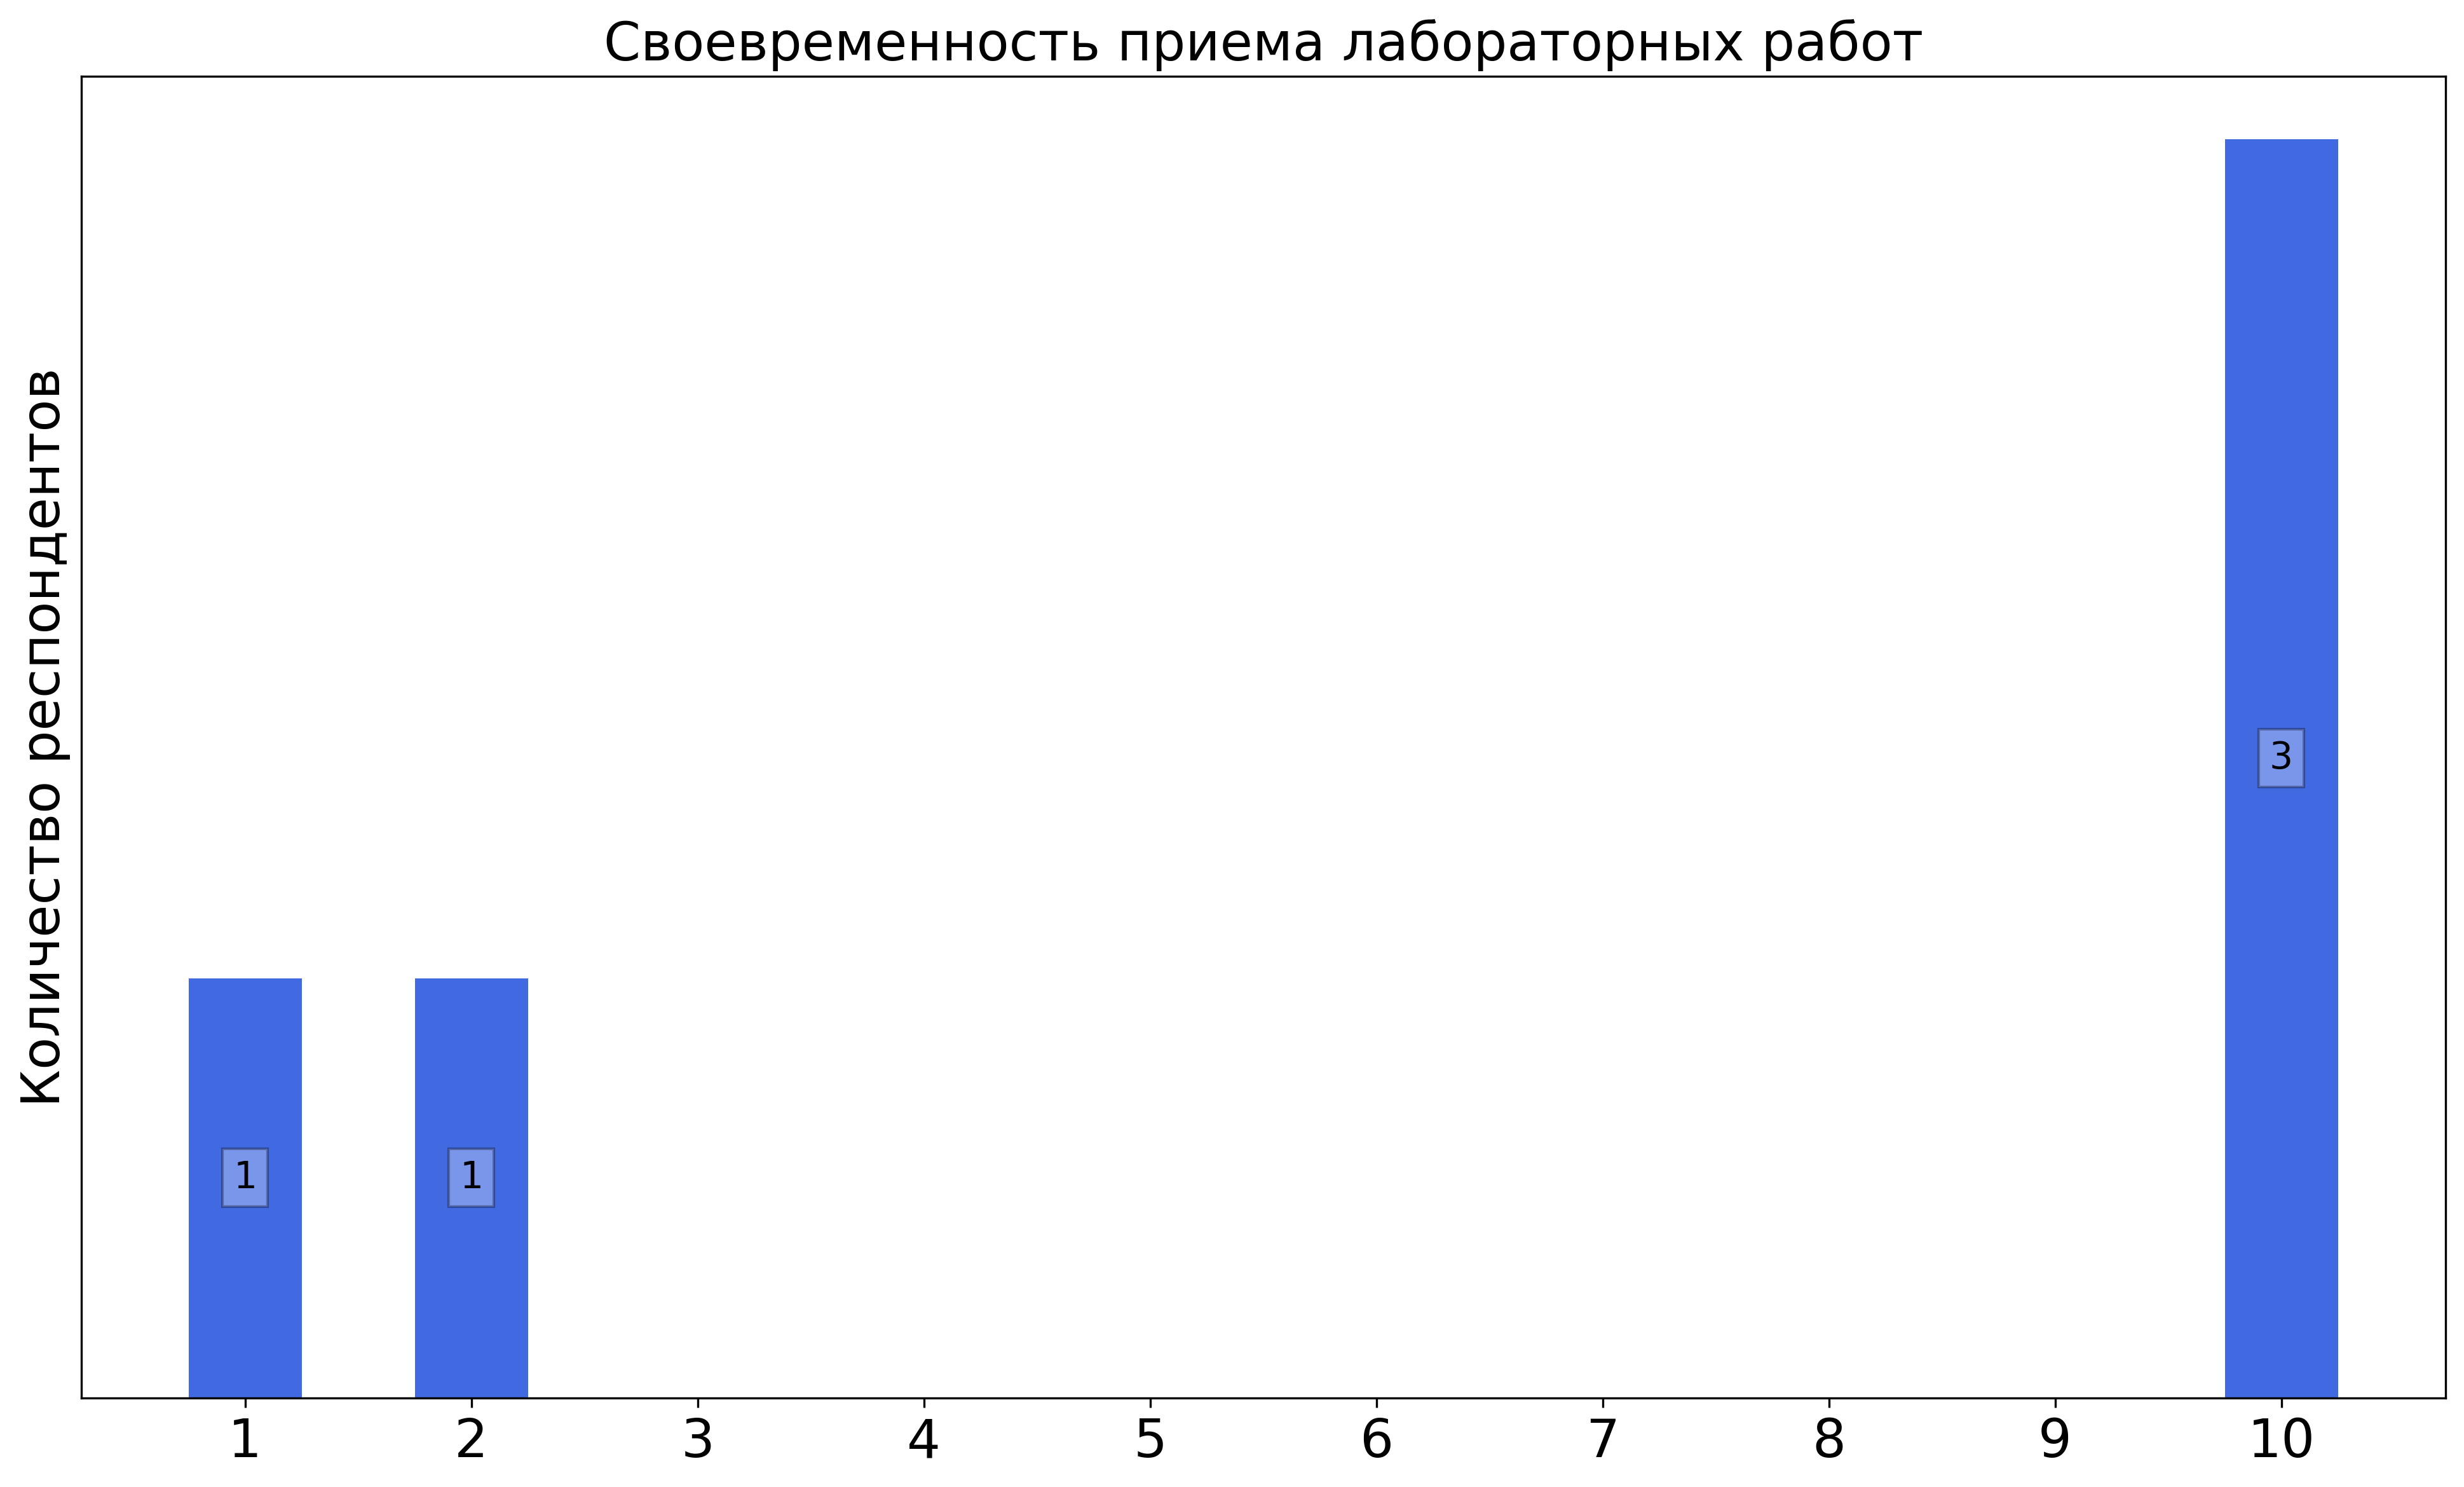
\includegraphics[width=\textwidth]{images/2 course/Радиотехнические цепи и сигналы/labniks-marks-Филатов И.В.-2.png}
            \end{subfigure}
            \begin{subfigure}[b]{0.45\textwidth}
                \centering
                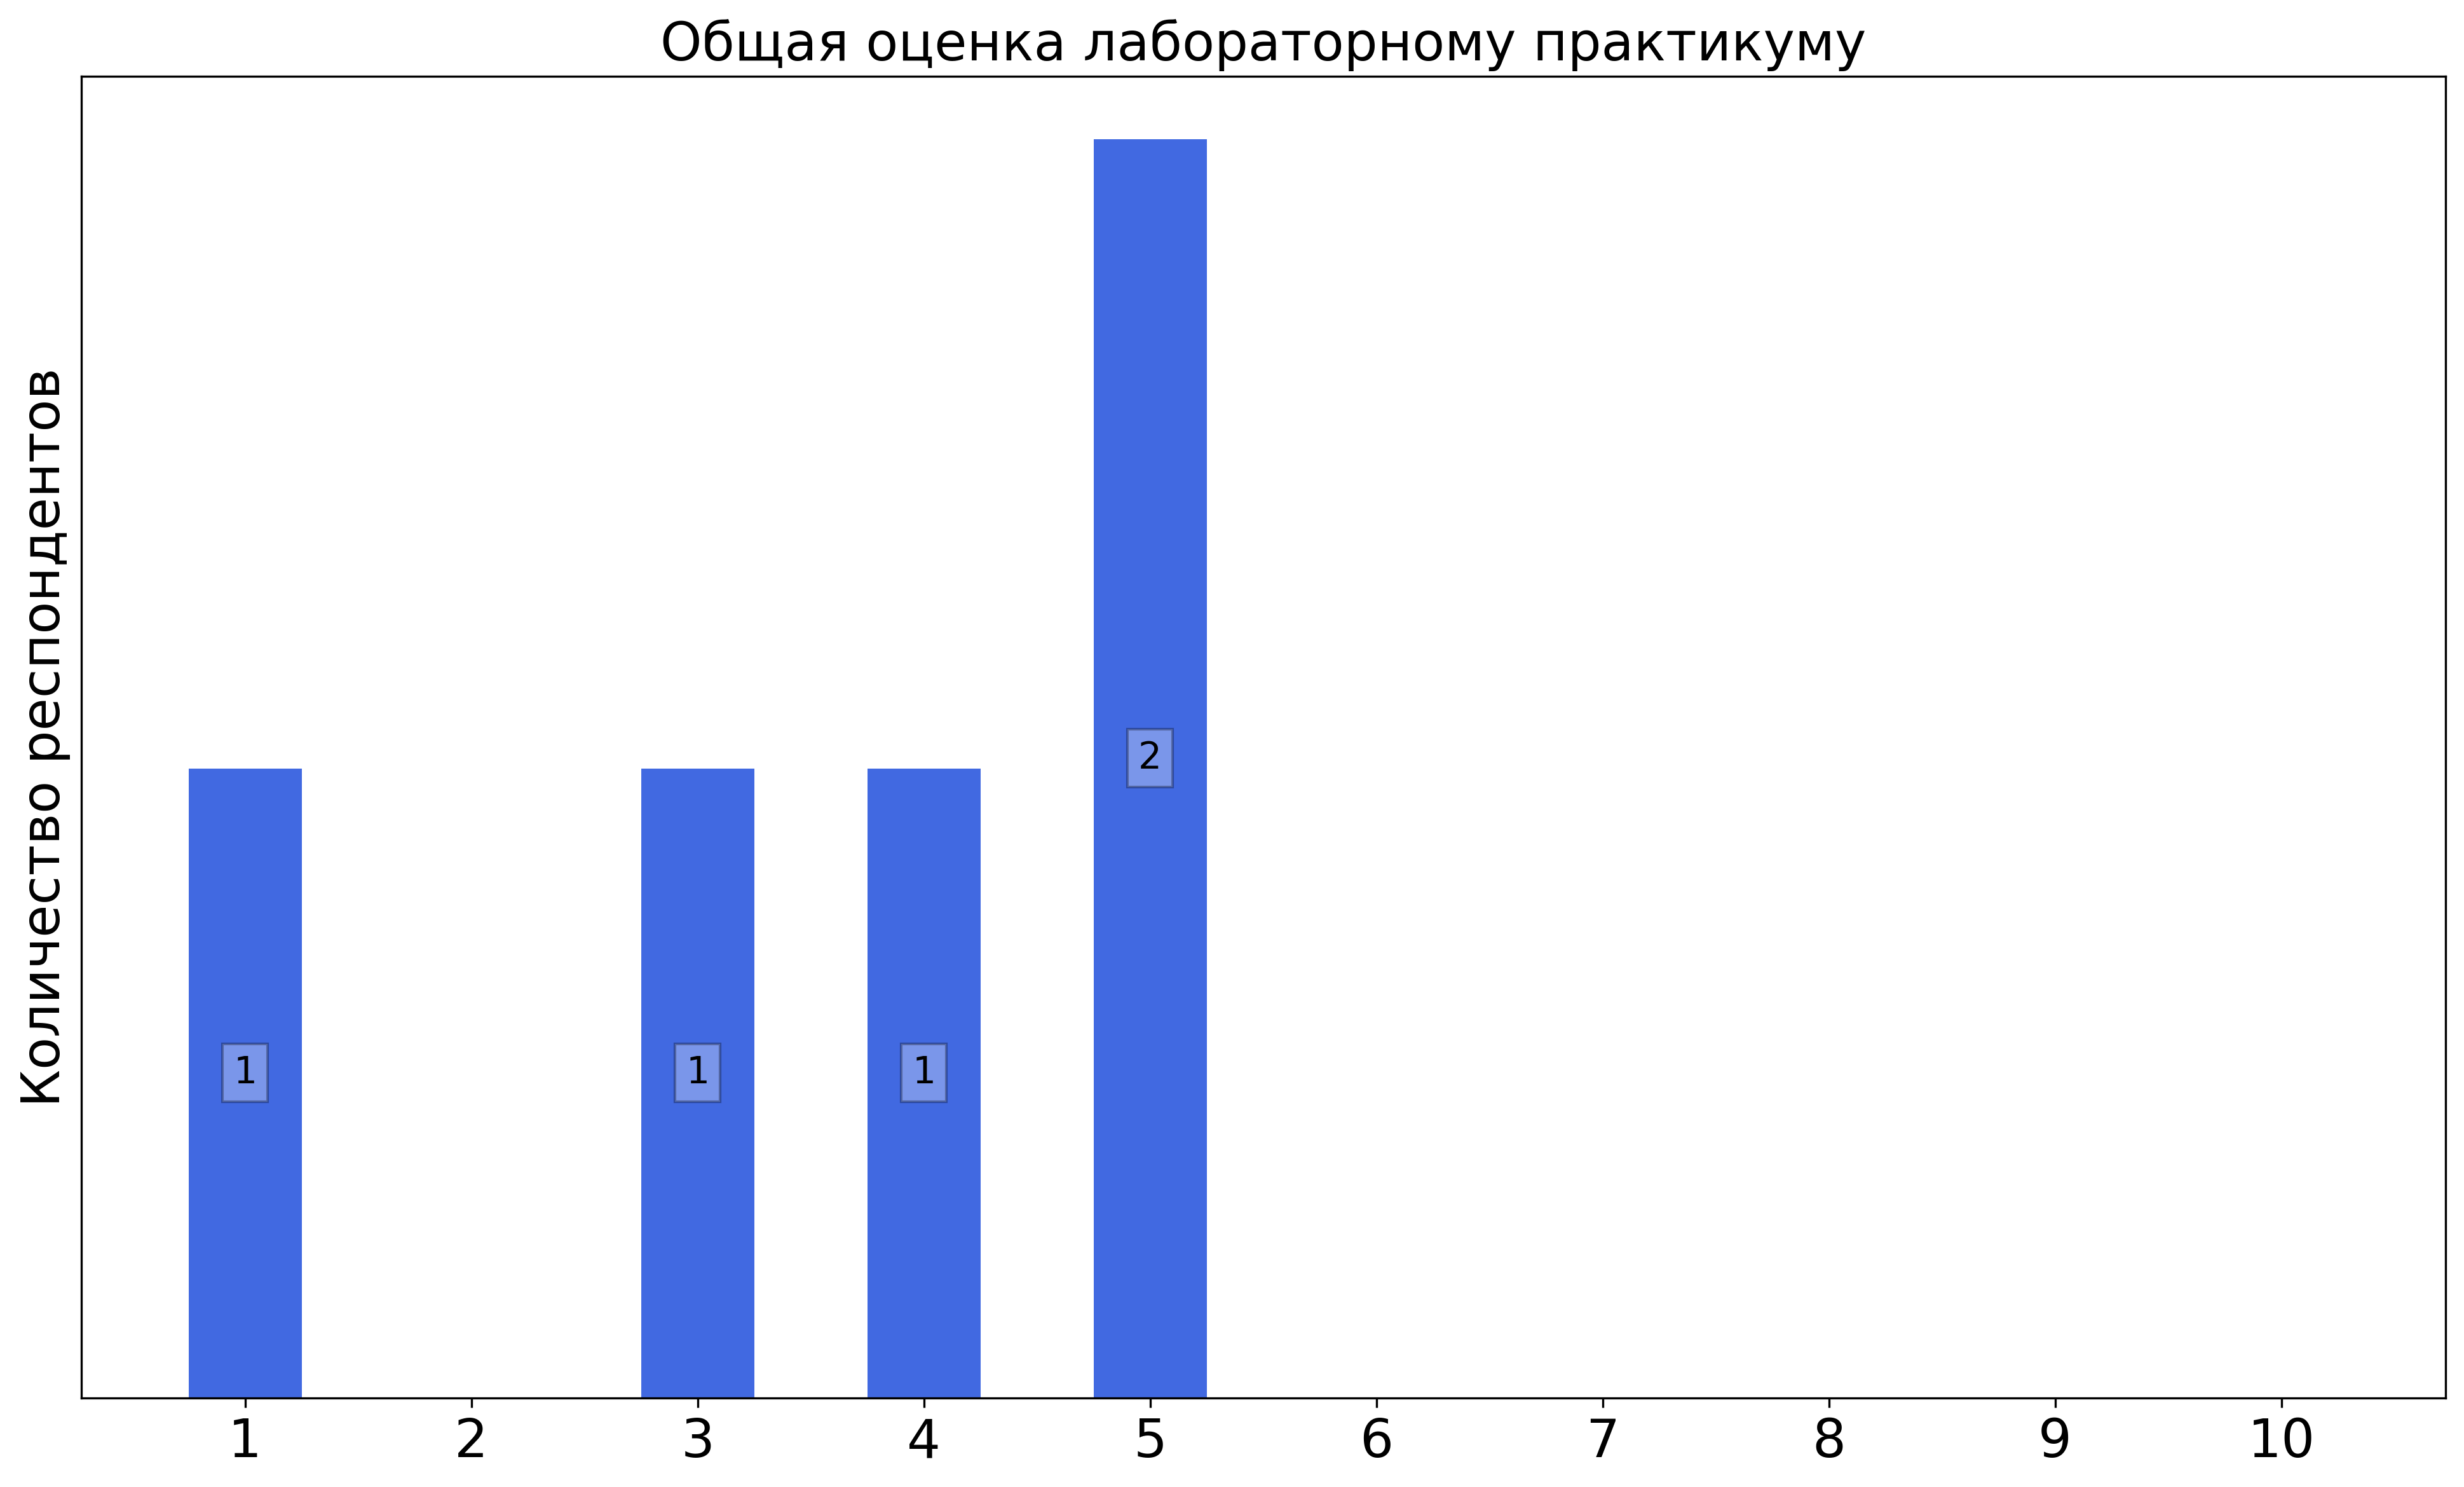
\includegraphics[width=\textwidth]{images/2 course/Радиотехнические цепи и сигналы/labniks-marks-Филатов И.В.-3.png}
            \end{subfigure}	
            \caption{Оценки респондентов о качестве преподавания лабораторных работ}
        \end{figure}

        \textbf{Комментарии студентов о преподавателе\protect\footnote{сохранены оригинальные орфография и пунктуация}}
        
            \begin{commentbox} 
                На лабораторных практикумах почти ничего не делал ибо почти все задания в микрокапе, а на сдачах оценка ставится по правилу -хор 5? -хор 5. Когда в соседнем кабинете Григорьев старший объяснял материал (кстати когда И.В. приходил позже, мы к нему на занятия ходили), у нас была только методичка по которой понять что-то было проблематично.
            \end{commentbox} 

        
    \subsubsection{Отзыв студентов о лабораторных работах. Преподаватель: Храмов Е.С.}
            \begin{figure}[H]
            \centering
            \begin{subfigure}[b]{0.45\textwidth}
                \centering
                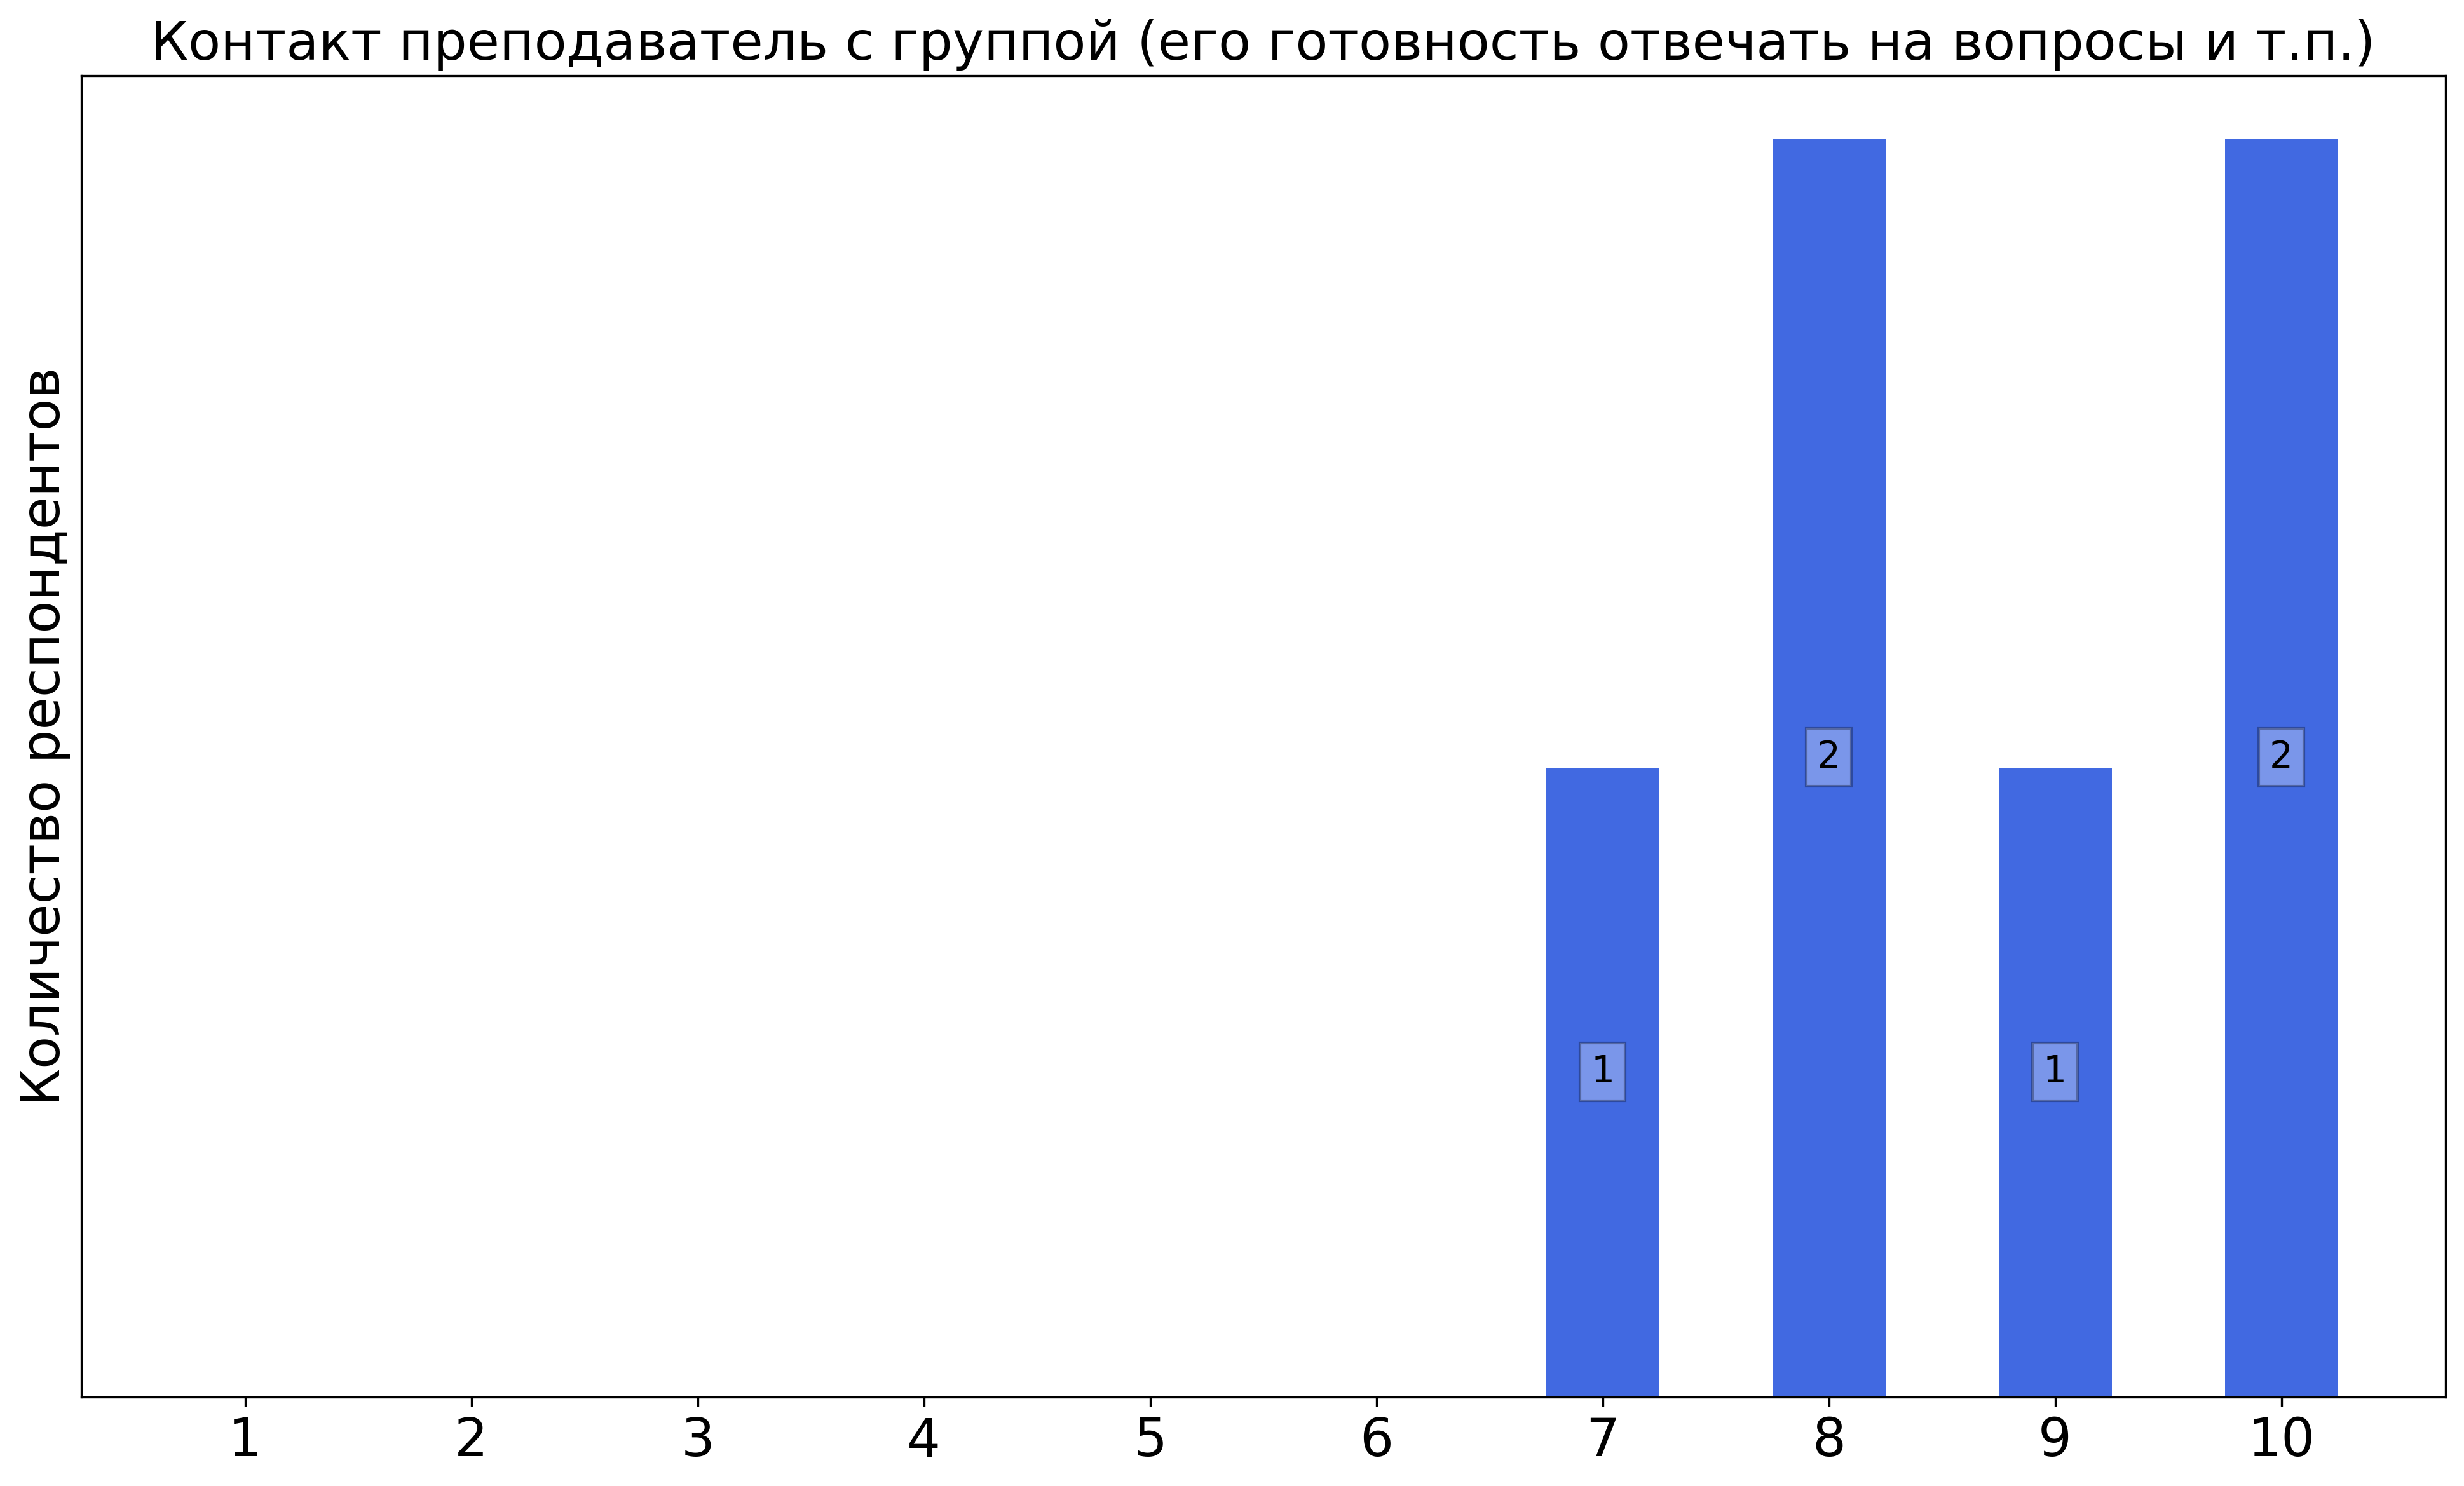
\includegraphics[width=\textwidth]{images/2 course/Радиотехнические цепи и сигналы/labniks-marks-Храмов Е.С.-0.png}
            \end{subfigure}
            \begin{subfigure}[b]{0.45\textwidth}
                \centering
                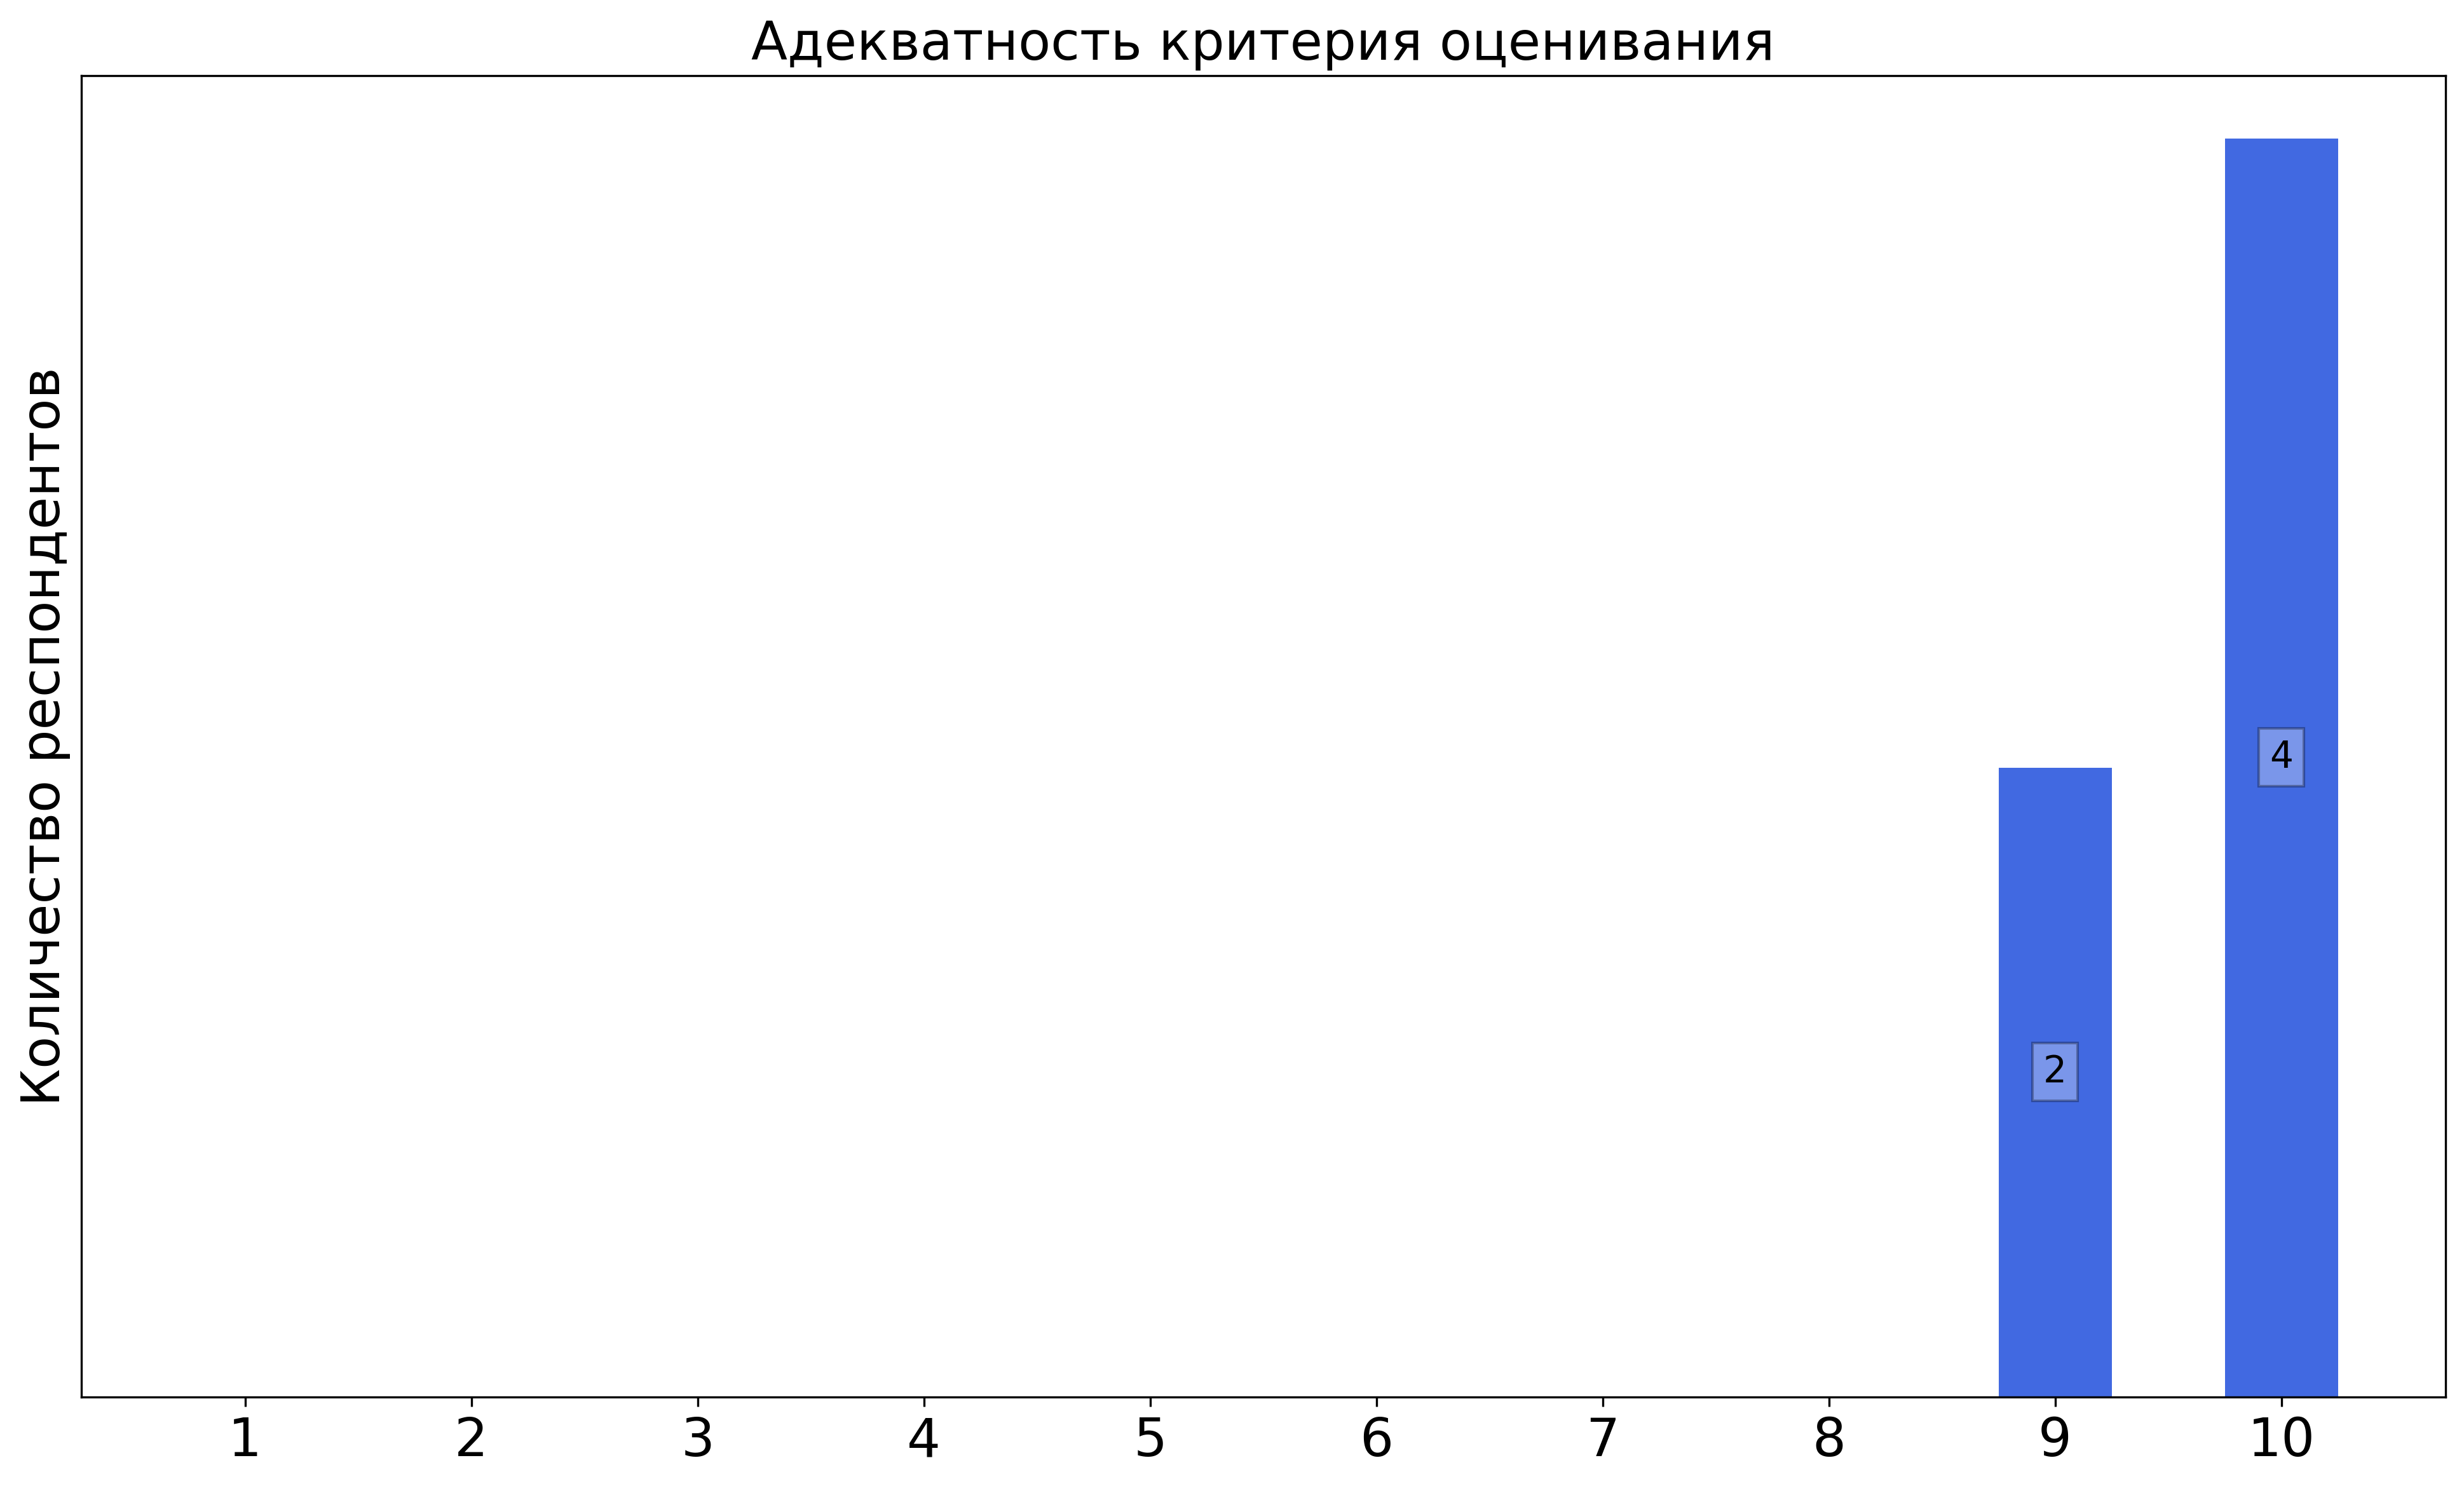
\includegraphics[width=\textwidth]{images/2 course/Радиотехнические цепи и сигналы/labniks-marks-Храмов Е.С.-1.png}
            \end{subfigure}
            \begin{subfigure}[b]{0.45\textwidth}
                \centering
                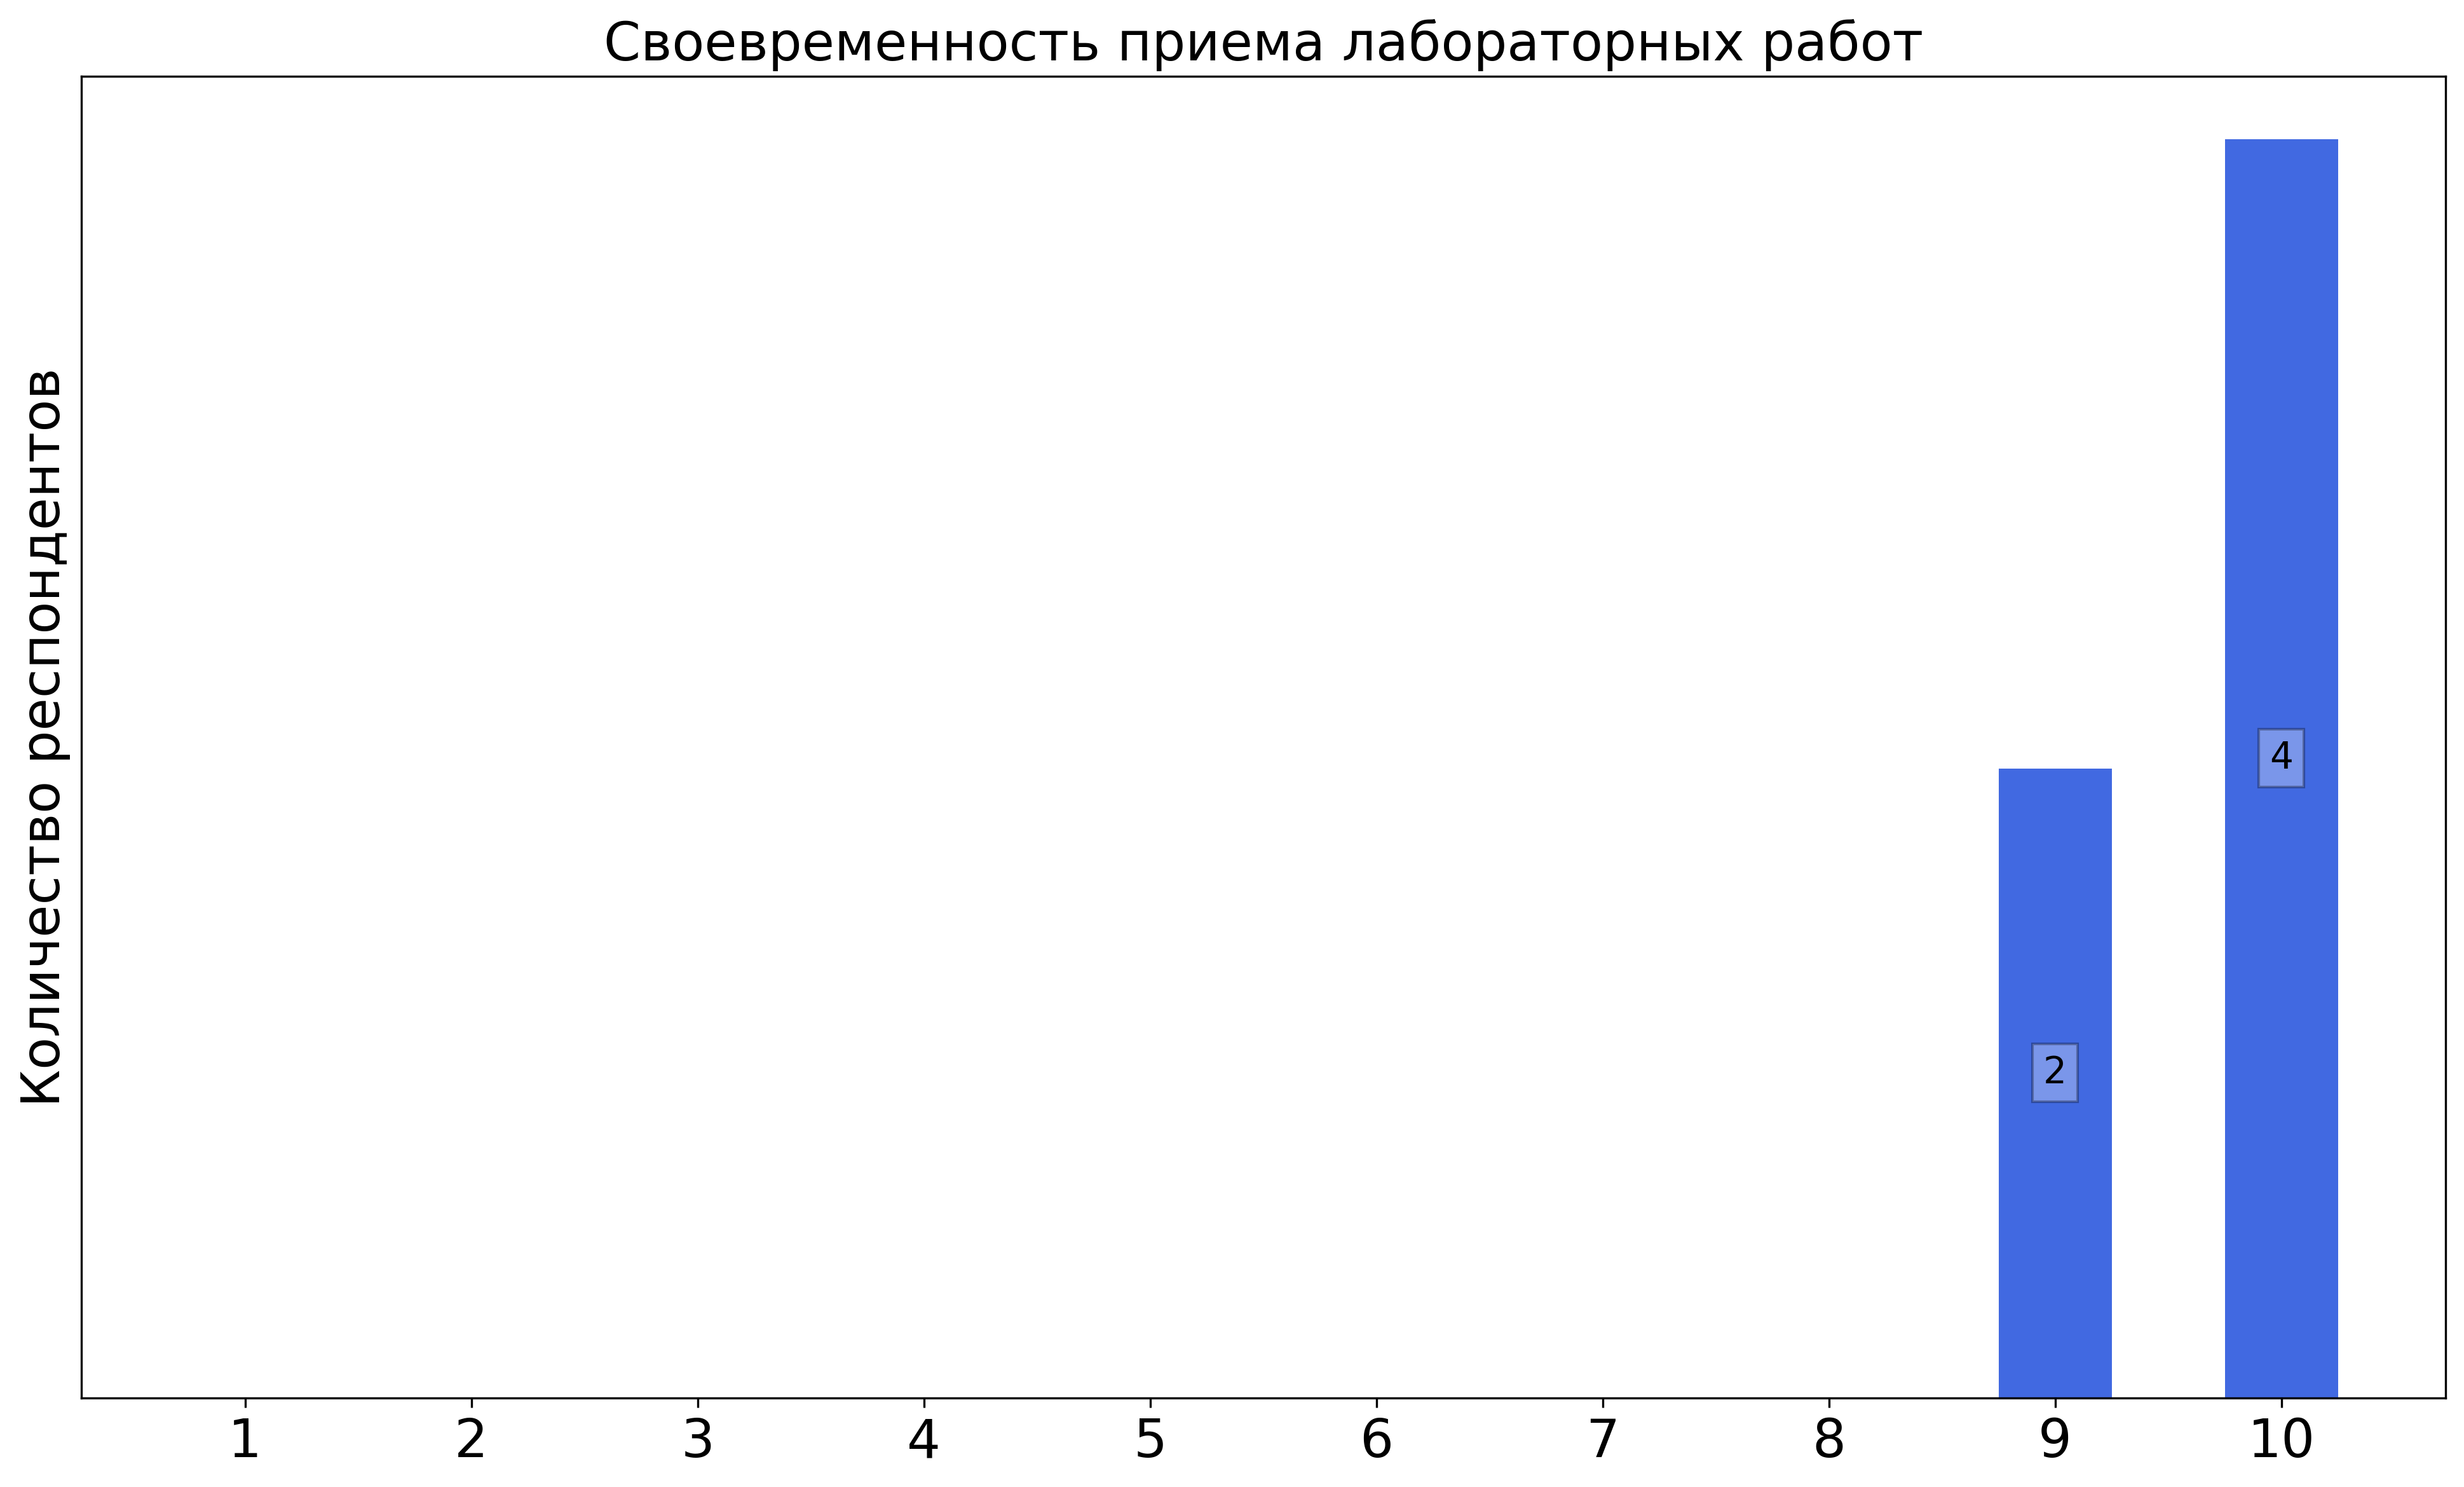
\includegraphics[width=\textwidth]{images/2 course/Радиотехнические цепи и сигналы/labniks-marks-Храмов Е.С.-2.png}
            \end{subfigure}
            \begin{subfigure}[b]{0.45\textwidth}
                \centering
                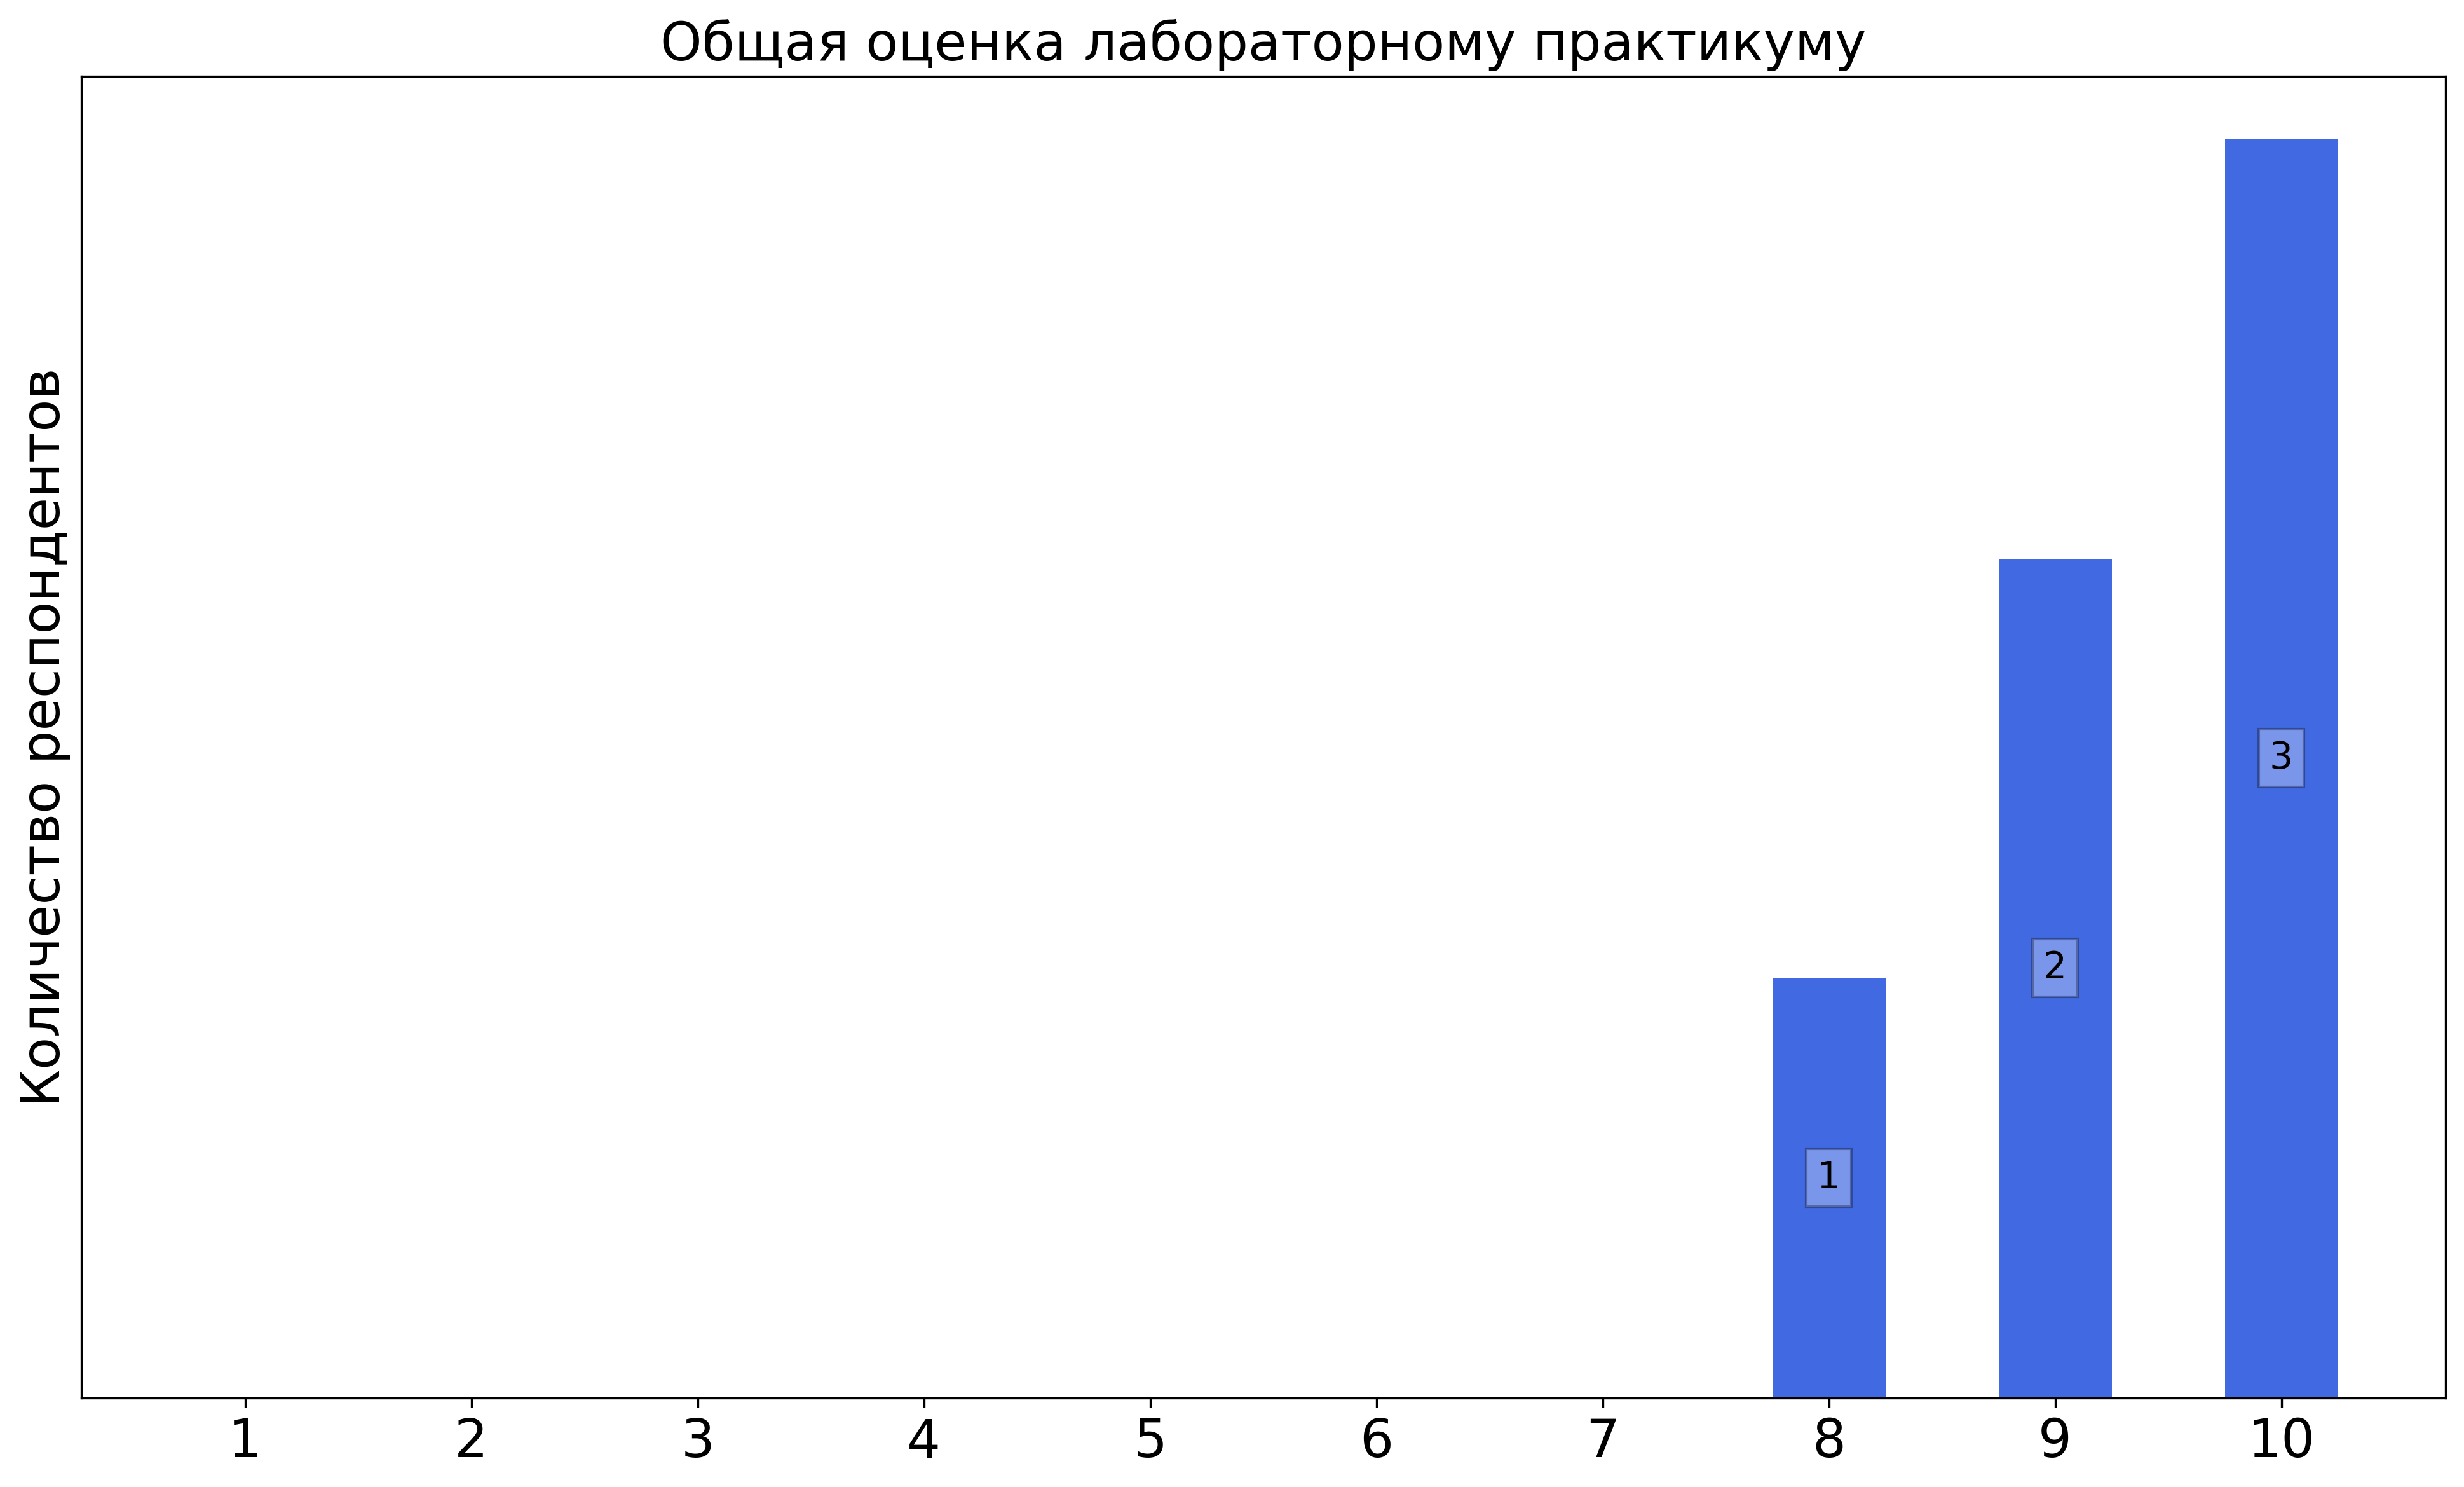
\includegraphics[width=\textwidth]{images/2 course/Радиотехнические цепи и сигналы/labniks-marks-Храмов Е.С.-3.png}
            \end{subfigure}	
            \caption{Оценки респондентов о качестве преподавания лабораторных работ}
        \end{figure}

        \textbf{Комментарии студентов о преподавателе\protect\footnote{сохранены оригинальные орфография и пунктуация}}
            \begin{commentbox} 
                Было недостаточно материалов в учебно-методических пособиях для освоения информации, изложенной в пособиях   
            \end{commentbox} 
        
            \begin{commentbox} 
                Замечательный молодой преподаватель, охотно работает с группой. 
            \end{commentbox} 

    
    \subsubsection{Прочие комментарии и предложения по улучшению курса}
        \begin{commentbox}
            Сделать экзамен обязательным для всех, а не только для тех, кому не повезло с семинаристом, или кто не был готов посещать бесполезные лекции ради автомата. Тогда и материалы нормальные появятся.
        \end{commentbox}

        \begin{commentbox}
            Сделать курс более структурированный и последовательным, при этом снабжая некоторые темы вводной информацией, касательно математических тем используемых в повествовании.
        \end{commentbox}

        \begin{commentbox}
            По всем предметам есть методички, кроме РТ цепей, поэтому даже рекомендованной литературы по которому идёт курс нету, а тех методичек, что выдают на каждую лабораторную работу, очевидно, не хватает материала.
        \end{commentbox}

        \begin{commentbox}
            Как то всё очень сумбурно происходило. Лекции посещались для выполнении задачки, не нашёл данный курс лекций полезным для себя. Курс лабораторных работ был сведён к большому количеству практических задач на теорвер. Мне понравилось.
        \end{commentbox}